\documentclass[]{book}
\usepackage{lmodern}
\usepackage{amssymb,amsmath}
\usepackage{ifxetex,ifluatex}
\usepackage{fixltx2e} % provides \textsubscript
\ifnum 0\ifxetex 1\fi\ifluatex 1\fi=0 % if pdftex
  \usepackage[T1]{fontenc}
  \usepackage[utf8]{inputenc}
\else % if luatex or xelatex
  \ifxetex
    \usepackage{mathspec}
  \else
    \usepackage{fontspec}
  \fi
  \defaultfontfeatures{Ligatures=TeX,Scale=MatchLowercase}
\fi
% use upquote if available, for straight quotes in verbatim environments
\IfFileExists{upquote.sty}{\usepackage{upquote}}{}
% use microtype if available
\IfFileExists{microtype.sty}{%
\usepackage{microtype}
\UseMicrotypeSet[protrusion]{basicmath} % disable protrusion for tt fonts
}{}
\usepackage[margin=1in]{geometry}
\usepackage{hyperref}
\hypersetup{unicode=true,
            pdftitle={EPsy 8252 Notes},
            pdfauthor={Andrew Zieffler},
            pdfborder={0 0 0},
            breaklinks=true}
\urlstyle{same}  % don't use monospace font for urls
\usepackage{natbib}
\bibliographystyle{plainnat}
\usepackage{color}
\usepackage{fancyvrb}
\newcommand{\VerbBar}{|}
\newcommand{\VERB}{\Verb[commandchars=\\\{\}]}
\DefineVerbatimEnvironment{Highlighting}{Verbatim}{commandchars=\\\{\}}
% Add ',fontsize=\small' for more characters per line
\usepackage{framed}
\definecolor{shadecolor}{RGB}{248,248,248}
\newenvironment{Shaded}{\begin{snugshade}}{\end{snugshade}}
\newcommand{\AlertTok}[1]{\textcolor[rgb]{0.94,0.16,0.16}{#1}}
\newcommand{\AnnotationTok}[1]{\textcolor[rgb]{0.56,0.35,0.01}{\textbf{\textit{#1}}}}
\newcommand{\AttributeTok}[1]{\textcolor[rgb]{0.77,0.63,0.00}{#1}}
\newcommand{\BaseNTok}[1]{\textcolor[rgb]{0.00,0.00,0.81}{#1}}
\newcommand{\BuiltInTok}[1]{#1}
\newcommand{\CharTok}[1]{\textcolor[rgb]{0.31,0.60,0.02}{#1}}
\newcommand{\CommentTok}[1]{\textcolor[rgb]{0.56,0.35,0.01}{\textit{#1}}}
\newcommand{\CommentVarTok}[1]{\textcolor[rgb]{0.56,0.35,0.01}{\textbf{\textit{#1}}}}
\newcommand{\ConstantTok}[1]{\textcolor[rgb]{0.00,0.00,0.00}{#1}}
\newcommand{\ControlFlowTok}[1]{\textcolor[rgb]{0.13,0.29,0.53}{\textbf{#1}}}
\newcommand{\DataTypeTok}[1]{\textcolor[rgb]{0.13,0.29,0.53}{#1}}
\newcommand{\DecValTok}[1]{\textcolor[rgb]{0.00,0.00,0.81}{#1}}
\newcommand{\DocumentationTok}[1]{\textcolor[rgb]{0.56,0.35,0.01}{\textbf{\textit{#1}}}}
\newcommand{\ErrorTok}[1]{\textcolor[rgb]{0.64,0.00,0.00}{\textbf{#1}}}
\newcommand{\ExtensionTok}[1]{#1}
\newcommand{\FloatTok}[1]{\textcolor[rgb]{0.00,0.00,0.81}{#1}}
\newcommand{\FunctionTok}[1]{\textcolor[rgb]{0.00,0.00,0.00}{#1}}
\newcommand{\ImportTok}[1]{#1}
\newcommand{\InformationTok}[1]{\textcolor[rgb]{0.56,0.35,0.01}{\textbf{\textit{#1}}}}
\newcommand{\KeywordTok}[1]{\textcolor[rgb]{0.13,0.29,0.53}{\textbf{#1}}}
\newcommand{\NormalTok}[1]{#1}
\newcommand{\OperatorTok}[1]{\textcolor[rgb]{0.81,0.36,0.00}{\textbf{#1}}}
\newcommand{\OtherTok}[1]{\textcolor[rgb]{0.56,0.35,0.01}{#1}}
\newcommand{\PreprocessorTok}[1]{\textcolor[rgb]{0.56,0.35,0.01}{\textit{#1}}}
\newcommand{\RegionMarkerTok}[1]{#1}
\newcommand{\SpecialCharTok}[1]{\textcolor[rgb]{0.00,0.00,0.00}{#1}}
\newcommand{\SpecialStringTok}[1]{\textcolor[rgb]{0.31,0.60,0.02}{#1}}
\newcommand{\StringTok}[1]{\textcolor[rgb]{0.31,0.60,0.02}{#1}}
\newcommand{\VariableTok}[1]{\textcolor[rgb]{0.00,0.00,0.00}{#1}}
\newcommand{\VerbatimStringTok}[1]{\textcolor[rgb]{0.31,0.60,0.02}{#1}}
\newcommand{\WarningTok}[1]{\textcolor[rgb]{0.56,0.35,0.01}{\textbf{\textit{#1}}}}
\usepackage{longtable,booktabs}
\usepackage{graphicx,grffile}
\makeatletter
\def\maxwidth{\ifdim\Gin@nat@width>\linewidth\linewidth\else\Gin@nat@width\fi}
\def\maxheight{\ifdim\Gin@nat@height>\textheight\textheight\else\Gin@nat@height\fi}
\makeatother
% Scale images if necessary, so that they will not overflow the page
% margins by default, and it is still possible to overwrite the defaults
% using explicit options in \includegraphics[width, height, ...]{}
\setkeys{Gin}{width=\maxwidth,height=\maxheight,keepaspectratio}
\IfFileExists{parskip.sty}{%
\usepackage{parskip}
}{% else
\setlength{\parindent}{0pt}
\setlength{\parskip}{6pt plus 2pt minus 1pt}
}
\setlength{\emergencystretch}{3em}  % prevent overfull lines
\providecommand{\tightlist}{%
  \setlength{\itemsep}{0pt}\setlength{\parskip}{0pt}}
\setcounter{secnumdepth}{5}
% Redefines (sub)paragraphs to behave more like sections
\ifx\paragraph\undefined\else
\let\oldparagraph\paragraph
\renewcommand{\paragraph}[1]{\oldparagraph{#1}\mbox{}}
\fi
\ifx\subparagraph\undefined\else
\let\oldsubparagraph\subparagraph
\renewcommand{\subparagraph}[1]{\oldsubparagraph{#1}\mbox{}}
\fi

%%% Use protect on footnotes to avoid problems with footnotes in titles
\let\rmarkdownfootnote\footnote%
\def\footnote{\protect\rmarkdownfootnote}

%%% Change title format to be more compact
\usepackage{titling}

% Create subtitle command for use in maketitle
\newcommand{\subtitle}[1]{
  \posttitle{
    \begin{center}\large#1\end{center}
    }
}

\setlength{\droptitle}{-2em}

  \title{EPsy 8252 Notes}
    \pretitle{\vspace{\droptitle}\centering\huge}
  \posttitle{\par}
    \author{Andrew Zieffler}
    \preauthor{\centering\large\emph}
  \postauthor{\par}
      \predate{\centering\large\emph}
  \postdate{\par}
    \date{2019-02-05}


\begin{document}
\maketitle

{
\setcounter{tocdepth}{1}
\tableofcontents
}
\begin{Shaded}
\begin{Highlighting}[]
\KeywordTok{install.packages}\NormalTok{(}\StringTok{"bookdown"}\NormalTok{)}
\CommentTok{# or the development version}
\CommentTok{# devtools::install_github("rstudio/bookdown")}

\KeywordTok{options}\NormalTok{(}\DataTypeTok{max.print =} \StringTok{"75"}\NormalTok{)}
\KeywordTok{options}\NormalTok{(}\DataTypeTok{scipen =} \DecValTok{5}\NormalTok{)}
\KeywordTok{options}\NormalTok{(}\DataTypeTok{digits =} \DecValTok{4}\NormalTok{)}
\KeywordTok{options}\NormalTok{(}\StringTok{"yaml.eval.expr"}\NormalTok{ =}\StringTok{ }\OtherTok{TRUE}\NormalTok{)}

\NormalTok{opts_chunk}\OperatorTok{$}\KeywordTok{set}\NormalTok{(}\DataTypeTok{prompt =} \OtherTok{FALSE}\NormalTok{, }\DataTypeTok{comment =} \OtherTok{NA}\NormalTok{, }\DataTypeTok{message =} \OtherTok{FALSE}\NormalTok{, }\DataTypeTok{warning =} \OtherTok{FALSE}\NormalTok{, }\DataTypeTok{tidy =} \OtherTok{FALSE}\NormalTok{, }\DataTypeTok{fig.align =} \StringTok{'center'}\NormalTok{)}
\NormalTok{opts_knit}\OperatorTok{$}\KeywordTok{set}\NormalTok{(}\DataTypeTok{width =} \DecValTok{85}\NormalTok{)}
\end{Highlighting}
\end{Shaded}

\hypertarget{introduction}{%
\chapter*{Introduction}\label{introduction}}
\addcontentsline{toc}{chapter}{Introduction}

This website includes the notes for \emph{EPsy 8252: Methods in Data Analysis for Educational Research II}. To download a ZIP file of the materials that make up this website (e.g., RMD files, HTML files) \href{https://github.com/zief0002/book-8252/archive/master.zip}{click here} or visit the \href{https://github.com/zief0002/book-8252}{github repository}.

The course website, which includes the syllabus, assignments, etc. can be found at \url{http://zief0002.github.io/epsy-8252/}

\hypertarget{rmarkdown}{%
\chapter{R Markdown}\label{rmarkdown}}

In this set of notes, you will learn how to integrate R syntax directly into your word-processed documents to create more reproducible reports.

\begin{center}\rule{0.5\linewidth}{\linethickness}\end{center}

\hypertarget{preparation}{%
\subsection*{Preparation}\label{preparation}}
\addcontentsline{toc}{subsection}{Preparation}

Before class you will need to do the following:

\begin{itemize}
\tightlist
\item
  Download the \href{https://github.com/zief0002/epsy-8252/raw/master/notes/s19-01-r-markdown/myBibliography.bib}{sample BibTeX file}
\item
  Download the CSL style file for the \href{https://www.zotero.org/styles}{American Psychological Association 6th edition (single-spaced bibliography)} from Zotero's repository.
\item
  Install the R package \textbf{tinytex}. See the \href{https://yihui.name/tinytex/}{documentation here}.
\end{itemize}

Read the following:

\begin{itemize}
\tightlist
\item
  \href{http://www.flutterbys.com.au/stats/tut/tut17.5.html\#h2_1}{Rmarkdown (and friends) Tutorial}
\end{itemize}

\begin{center}\rule{0.5\linewidth}{\linethickness}\end{center}

\hypertarget{notes}{%
\section{Notes}\label{notes}}

The notes and files you will need can be found at:

\begin{itemize}
\tightlist
\item
  \href{https://github.com/zief0002/book-8252/raw/master/s19-01-r-markdown/01-r-markdown.pdf}{Unit 01: R Markdown} {[}Class Notes{]}
\end{itemize}

\hypertarget{other-resources}{%
\section{Other Resources}\label{other-resources}}

In addition to the notes and what we cover in class, there many other resources for learning about R Markdown. Here are some resources that may be helpful in that endeavor:

\begin{itemize}
\tightlist
\item
  \href{http://rmarkdown.rstudio.com/}{R Markdown documentation:} Official R Markdown documentation from RStudio
\item
  \href{https://www.rstudio.com/wp-content/uploads/2015/02/rmarkdown-cheatsheet.pdf}{R Markdown cheatsheet:} What it sounds like; a cheatsheet for R Markdown
\item
  \href{http://yihui.name/knitr/}{knitr:} Document and code chunk options for R Markdown
\item
  \href{https://rmarkdown.rstudio.com/gallery.html}{R Markdown Gallery:} - Gallery of some R Markdown outputs
\item
  \href{https://holtzy.github.io/Pimp-my-rmd/}{Pimp my Rmd:} Blog post providing a few tips to improve the appearance of output documents.
\end{itemize}

For \textbf{typesetting equations} using R Markdown, check out:

\begin{itemize}
\tightlist
\item
  \href{https://en.wikibooks.org/wiki/LaTeX/Mathematics}{Using LaTeX to write mathematical content}
\end{itemize}

For integrating \textbf{references} into R Markdown, here are a few resources:

\begin{itemize}
\tightlist
\item
  \href{https://www.zotero.org/styles}{Zotero CSL style repository}
\item
  \href{http://blog.mendeley.com/2012/03/24/how-to-series-generate-bibtex-files-for-your-collections-for-use-in-latex-part-3-of-12/}{Export a BibTeX file from Mendeley}
\item
  \href{http://libguides.mit.edu/c.php?g=176000\&p=1159208\#3}{Export a BibTeX file from Zotero}
\end{itemize}

Here are some references for using reveal.js and remark.js to create sweet-looking \textbf{presentations}:

\begin{itemize}
\tightlist
\item
  \href{http://rmarkdown.rstudio.com/revealjs_presentation_format.html}{Reveal.js presentations}
\item
  \href{https://logfc.wordpress.com/2015/06/24/presentations-in-rmarkdown/}{Customizing Reveal.js presentations}
\item
  \href{https://github.com/yihui/xaringan}{xaringan}
\end{itemize}

Finally here are some other tools for using Markdown in academia:

\begin{itemize}
\tightlist
\item
  Create a poster with the \href{https://github.com/brentthorne/posterdown}{posterdown package}
\end{itemize}

\hypertarget{pretty-printing-tables-in-markdown}{%
\chapter*{Pretty-Printing Tables in Markdown}\label{pretty-printing-tables-in-markdown}}
\addcontentsline{toc}{chapter}{Pretty-Printing Tables in Markdown}

Often it is useful to format table output to make it look good or to adhere a particular style (e.g., APA). There are several packages that help in this endeavor when working in an Rmarkdown document. Below the primary tools used are:

\begin{itemize}
\tightlist
\item
  The \texttt{kable()} function from the \textbf{knitr} package; and
\item
  Functions from the \textbf{kableExtra} package.
\end{itemize}

Other packages for formatting tables, among others, include the \href{https://gt.rstudio.com/}{gt package}, the \href{https://hughjonesd.github.io/huxtable/}{huxtable package}, and the \href{https://gdemin.github.io/expss/}{expss package}. For complete APA formatting check out the \href{https://crsh.github.io/papaja_man/}{papaja package}.

The primary input to the \texttt{kable()} function is a data frame. This data frame will include the primary contents for you table. A data frame can either be created as the ouput of a function or directly using the \texttt{data.frame()} function. Below I will create and format a couple different common tables produced for statistical reports. To do so, I will use data from \emph{ed-schools-2018.csv} file (see the \protect\hyperlink{ed-schools-2018}{data codebook} here). These data include institutional-level attributes for several graduate education schools/programs rated by \emph{U.S. News and World Report} in 2018.

\begin{Shaded}
\begin{Highlighting}[]
\CommentTok{# Load libraries}
\KeywordTok{library}\NormalTok{(AICcmodavg)}
\KeywordTok{library}\NormalTok{(broom)}
\KeywordTok{library}\NormalTok{(corrr)}
\KeywordTok{library}\NormalTok{(dplyr)}
\KeywordTok{library}\NormalTok{(knitr)}
\KeywordTok{library}\NormalTok{(kableExtra)}
\KeywordTok{library}\NormalTok{(readr)}
\KeywordTok{library}\NormalTok{(tidyr)}

\CommentTok{# Read in data}
\NormalTok{ed =}\StringTok{ }\KeywordTok{read_csv}\NormalTok{(}\DataTypeTok{file =} \StringTok{"~/Documents/github/epsy-8252/data/ed-schools-2018.csv"}\NormalTok{)}

\CommentTok{# Drop rows with missing data}
\NormalTok{educ =}\StringTok{ }\NormalTok{ed }\OperatorTok
\StringTok{  }\KeywordTok{drop_na}\NormalTok{()}

\CommentTok{# Create log-transformed variables}
\NormalTok{educ =}\StringTok{ }\NormalTok{educ }\OperatorTok
\StringTok{  }\KeywordTok{mutate}\NormalTok{(}
    \DataTypeTok{Lpeer =} \KeywordTok{log}\NormalTok{(peer),}
    \DataTypeTok{Ldoc_accept =} \KeywordTok{log}\NormalTok{(doc_accept),}
    \DataTypeTok{Lenroll =} \KeywordTok{log}\NormalTok{(enroll)}
\NormalTok{    )}
\end{Highlighting}
\end{Shaded}

\hypertarget{summary-statistics-table}{%
\section*{Summary Statistics Table}\label{summary-statistics-table}}
\addcontentsline{toc}{section}{Summary Statistics Table}

Say we wanted to produce a table of means and standard deviations for the variables: \texttt{peer}, \texttt{doc\_accept}, and \texttt{enroll}. Furthermore, we want these for both the raw (untransformed) and log-transformed versions of these variables. Here is a sketch of what the table should look like:

{[}INSERT SKETCH{]}

To begin we will set up a data frame that includes the information from the table. We do this manually to illustrate use of the \texttt{data.frame()} function to set up a data frame.

\begin{Shaded}
\begin{Highlighting}[]
\NormalTok{tab_}\DecValTok{01}\NormalTok{ =}\StringTok{ }\KeywordTok{data.frame}\NormalTok{(}
  \DataTypeTok{Measure =} \KeywordTok{c}\NormalTok{(}\StringTok{"Peer rating"}\NormalTok{, }\StringTok{"Ph.D. acceptance rate"}\NormalTok{, }\StringTok{"Enrollment"}\NormalTok{),}
  \DataTypeTok{M_1  =} \KeywordTok{c}\NormalTok{(}\KeywordTok{mean}\NormalTok{(educ}\OperatorTok{$}\NormalTok{peer), }\KeywordTok{mean}\NormalTok{(educ}\OperatorTok{$}\NormalTok{doc_accept), }\KeywordTok{mean}\NormalTok{(educ}\OperatorTok{$}\NormalTok{enroll)),}
  \DataTypeTok{SD_1 =} \KeywordTok{c}\NormalTok{(}\KeywordTok{sd}\NormalTok{(educ}\OperatorTok{$}\NormalTok{peer), }\KeywordTok{sd}\NormalTok{(educ}\OperatorTok{$}\NormalTok{doc_accept), }\KeywordTok{sd}\NormalTok{(educ}\OperatorTok{$}\NormalTok{enroll)),}
  \DataTypeTok{M_2  =} \KeywordTok{c}\NormalTok{(}\KeywordTok{mean}\NormalTok{(educ}\OperatorTok{$}\NormalTok{Lpeer), }\KeywordTok{mean}\NormalTok{(educ}\OperatorTok{$}\NormalTok{Ldoc_accept), }\KeywordTok{mean}\NormalTok{(educ}\OperatorTok{$}\NormalTok{Lenroll)),}
  \DataTypeTok{SD_2 =} \KeywordTok{c}\NormalTok{(}\KeywordTok{sd}\NormalTok{(educ}\OperatorTok{$}\NormalTok{Lpeer), }\KeywordTok{sd}\NormalTok{(educ}\OperatorTok{$}\NormalTok{Ldoc_accept), }\KeywordTok{sd}\NormalTok{(educ}\OperatorTok{$}\NormalTok{Lenroll))}
\NormalTok{)}

\NormalTok{tab_}\DecValTok{01}
\end{Highlighting}
\end{Shaded}

\begin{verbatim}
                Measure        M_1        SD_1      M_2      SD_2
1           Peer rating   3.312295   0.4893203 1.187198 0.1439847
2 Ph.D. acceptance rate  40.113115  20.2276300 3.525419 0.6461164
3            Enrollment 969.762295 664.9454219 6.657939 0.7228670
\end{verbatim}

We can now use the \texttt{kable()} function to rename the columns, round the numeric values, and set a caption.

\begin{Shaded}
\begin{Highlighting}[]
\KeywordTok{kable}\NormalTok{(}
\NormalTok{  tab_}\DecValTok{01}\NormalTok{,}
  \DataTypeTok{col.names =} \KeywordTok{c}\NormalTok{(}\StringTok{"Measure"}\NormalTok{, }\StringTok{"*M*"}\NormalTok{, }\StringTok{"*SD*"}\NormalTok{, }\StringTok{"*M*"}\NormalTok{, }\StringTok{"*SD*"}\NormalTok{),}
  \DataTypeTok{digits =} \DecValTok{2}\NormalTok{,}
  \DataTypeTok{caption =} \StringTok{"Means and Standard Deviations of Three Measures of Graduate Programs of Education ($n=122$)"}
\NormalTok{  )}
\end{Highlighting}
\end{Shaded}

\label{tab:unnamed-chunk-11}Means and Standard Deviations of Three Measures of Graduate Programs of Education (\(n=122\))

Measure

\emph{M}

\emph{SD}

\emph{M}

\emph{SD}

Peer rating

3.31

0.49

1.19

0.14

Ph.D.~acceptance rate

40.11

20.23

3.53

0.65

Enrollment

969.76

664.95

6.66

0.72

Finally, we use functions from the \textbf{kableExtra} package to add our top header row.

\begin{Shaded}
\begin{Highlighting}[]
\KeywordTok{kable}\NormalTok{(}
\NormalTok{  tab_}\DecValTok{01}\NormalTok{,}
  \DataTypeTok{col.names =} \KeywordTok{c}\NormalTok{(}\StringTok{"Measure"}\NormalTok{, }\StringTok{"*M*"}\NormalTok{, }\StringTok{"*SD*"}\NormalTok{, }\StringTok{"*M*"}\NormalTok{, }\StringTok{"*SD*"}\NormalTok{),}
  \DataTypeTok{align =} \KeywordTok{c}\NormalTok{(}\StringTok{"l"}\NormalTok{, }\StringTok{"c"}\NormalTok{, }\StringTok{"c"}\NormalTok{, }\StringTok{"c"}\NormalTok{, }\StringTok{"c"}\NormalTok{),}
  \DataTypeTok{digits =} \DecValTok{2}\NormalTok{,}
  \DataTypeTok{caption =} \StringTok{"Means and Standard Deviations of Three Measures of Graduate Programs of Education ($n=122$)"}
\NormalTok{  ) }\OperatorTok
\StringTok{  }\KeywordTok{add_header_above}\NormalTok{(}
    \DataTypeTok{header =} \KeywordTok{c}\NormalTok{(}\StringTok{" "}\NormalTok{ =}\StringTok{ }\DecValTok{1}\NormalTok{, }\StringTok{"Untransformed"}\NormalTok{ =}\StringTok{ }\DecValTok{2}\NormalTok{, }\StringTok{"Log-transformed"}\NormalTok{ =}\StringTok{ }\DecValTok{2}\NormalTok{)}
\NormalTok{    ) }\OperatorTok
\StringTok{  }\KeywordTok{footnote}\NormalTok{(}
    \DataTypeTok{general =} \StringTok{"Variables were log-transformed using the natural logarithm."}\NormalTok{,}
    \DataTypeTok{general_title =} \StringTok{"Note."}\NormalTok{,}
    \DataTypeTok{footnote_as_chunk =} \OtherTok{TRUE}
\NormalTok{    )}
\end{Highlighting}
\end{Shaded}

\label{tab:unnamed-chunk-12}Means and Standard Deviations of Three Measures of Graduate Programs of Education (\(n=122\))

Untransformed

Log-transformed

Measure

\emph{M}

\emph{SD}

\emph{M}

\emph{SD}

Peer rating

3.31

0.49

1.19

0.14

Ph.D.~acceptance rate

40.11

20.23

3.53

0.65

Enrollment

969.76

664.95

6.66

0.72

{Note.} Variables were log-transformed using the natural logarithm.

\hypertarget{correlation-table}{%
\section*{Correlation Table}\label{correlation-table}}
\addcontentsline{toc}{section}{Correlation Table}

For our second example, say we wanted to produce a table of pairwise correlations for the variables: \texttt{peer}, \texttt{doc\_accept}, and \texttt{enroll}. To begin we will again set up a data frame, but this time we will generate it using functions from the \textbf{corrr} package.

\begin{Shaded}
\begin{Highlighting}[]
\NormalTok{tab_}\DecValTok{02}\NormalTok{ =}\StringTok{ }\NormalTok{educ }\OperatorTok
\StringTok{  }\KeywordTok{select}\NormalTok{(peer, doc_accept, enroll) }\OperatorTok
\StringTok{  }\KeywordTok{correlate}\NormalTok{() }\OperatorTok
\StringTok{  }\KeywordTok{shave}\NormalTok{(}\DataTypeTok{upper =} \OtherTok{TRUE}\NormalTok{) }\OperatorTok
\StringTok{  }\KeywordTok{fashion}\NormalTok{(}\DataTypeTok{decimals =} \DecValTok{2}\NormalTok{, }\DataTypeTok{na_print =} \StringTok{"—"}\NormalTok{) }

\NormalTok{tab_}\DecValTok{02}
\end{Highlighting}
\end{Shaded}

\begin{verbatim}
     rowname peer doc_accept enroll
1       peer    —          —      —
2 doc_accept -.54          —      —
3     enroll  .10       -.03      —
\end{verbatim}

Now we change the values in the \texttt{rownames} column by mutating in new values, and pipe this into the \texttt{kable()} function, where we will change the column name and add a caption. Keeping the default alignment will align the decimal points within columns.

\begin{Shaded}
\begin{Highlighting}[]
\NormalTok{tab_}\DecValTok{02} \OperatorTok
\StringTok{  }\KeywordTok{mutate}\NormalTok{(}
    \DataTypeTok{rowname =} \KeywordTok{c}\NormalTok{(}\StringTok{"1. Peer rating"}\NormalTok{, }\StringTok{"2. Ph.D. acceptance rate"}\NormalTok{, }\StringTok{"3. Enrollment"}\NormalTok{)}
\NormalTok{  ) }\OperatorTok
\StringTok{  }\KeywordTok{kable}\NormalTok{(}
    \DataTypeTok{caption =} \StringTok{"Correlations between Three Measures of Graduate Programs of Education"}\NormalTok{,}
    \DataTypeTok{col.names =} \KeywordTok{c}\NormalTok{(}\StringTok{"Measure"}\NormalTok{, }\StringTok{"1"}\NormalTok{, }\StringTok{"2"}\NormalTok{, }\StringTok{"3"}\NormalTok{)}
\NormalTok{  )}
\end{Highlighting}
\end{Shaded}

\label{tab:unnamed-chunk-15}Correlations between Three Measures of Graduate Programs of Education

Measure

1

2

3

\begin{enumerate}
\def\labelenumi{\arabic{enumi}.}
\tightlist
\item
  Peer rating

  ---

  ---

  ---

  \begin{enumerate}
  \def\labelenumii{\arabic{enumii}.}
  \setcounter{enumii}{1}
  \tightlist
  \item
    Ph.D.~acceptance rate

    -.54

    ---

    ---

    \begin{enumerate}
    \def\labelenumiii{\arabic{enumiii}.}
    \setcounter{enumiii}{2}
    \tightlist
    \item
      Enrollment

      .10

      -.03

      ---
    \end{enumerate}
  \end{enumerate}
\end{enumerate}

\hypertarget{regression-table-single-model}{%
\section*{Regression Table: Single Model}\label{regression-table-single-model}}
\addcontentsline{toc}{section}{Regression Table: Single Model}

It is common to report the coefficient-level information from a fitted regression model in a table. The nice thing about using the \texttt{tidy()} function to obtain coefficient-level information from a fitted model is that the output is formatted as a data frame. Thus, we can use the output from \texttt{tidy()} directly in the \texttt{kable()} function. Below I fit a regression model and then use piping to obtain the coefficient-level information and create the table.

\begin{Shaded}
\begin{Highlighting}[]
\KeywordTok{lm}\NormalTok{(peer }\OperatorTok{~}\StringTok{ }\DecValTok{1} \OperatorTok{+}\StringTok{ }\NormalTok{doc_accept }\OperatorTok{+}\StringTok{ }\NormalTok{gre_verbal, }\DataTypeTok{data =}\NormalTok{ educ) }\OperatorTok
\StringTok{  }\KeywordTok{tidy}\NormalTok{() }\OperatorTok
\StringTok{  }\KeywordTok{kable}\NormalTok{()}
\end{Highlighting}
\end{Shaded}

term

estimate

std.error

statistic

p.value

(Intercept)

-1.5268

1.6668

-0.916

0.3615

doc\_accept

-0.0107

0.0019

-5.519

0.0000

gre\_verbal

0.0340

0.0106

3.221

0.0016

To format this, we might want to change the column names and round the numerical information to a better number of digits; typically \emph{p}-values are rounded to three decimal places and coefficients, standard errors and \emph{t}-values are rounded to two digits.

\begin{Shaded}
\begin{Highlighting}[]
\KeywordTok{lm}\NormalTok{(peer }\OperatorTok{~}\StringTok{ }\DecValTok{1} \OperatorTok{+}\StringTok{ }\NormalTok{doc_accept }\OperatorTok{+}\StringTok{ }\NormalTok{gre_verbal, }\DataTypeTok{data =}\NormalTok{ educ) }\OperatorTok
\StringTok{  }\KeywordTok{tidy}\NormalTok{() }\OperatorTok
\StringTok{  }\KeywordTok{kable}\NormalTok{(}
    \DataTypeTok{caption =} \StringTok{"Coefficient-Level Estimates for a Model Fitted to Estimate Variation in Peer Ratings."}\NormalTok{,}
    \DataTypeTok{col.names =} \KeywordTok{c}\NormalTok{(}\StringTok{"Predictor"}\NormalTok{, }\StringTok{"B"}\NormalTok{, }\StringTok{"SE"}\NormalTok{, }\StringTok{"t"}\NormalTok{, }\StringTok{"p"}\NormalTok{),}
    \DataTypeTok{digits =} \KeywordTok{c}\NormalTok{(}\DecValTok{0}\NormalTok{, }\DecValTok{2}\NormalTok{, }\DecValTok{3}\NormalTok{, }\DecValTok{2}\NormalTok{, }\DecValTok{3}\NormalTok{)}
\NormalTok{  )}
\end{Highlighting}
\end{Shaded}

\label{tab:unnamed-chunk-17}Coefficient-Level Estimates for a Model Fitted to Estimate Variation in Peer Ratings.

Predictor

B

SE

t

p

(Intercept)

-1.53

1.667

-0.92

0.362

doc\_accept

-0.01

0.002

-5.52

0.000

gre\_verbal

0.03

0.011

3.22

0.002

Last things to fix are the predictor names and the \emph{p}-values. The rounding of the \emph{p}-values has rendered them as zero. We can use the \texttt{pvalue()} function from the \textbf{scales} package to better format the column of \emph{p}-values. This is carried out prior to piping the output into the \texttt{kable()} function by changing the values in the \texttt{p.value} column. (Note that rather than load a package for a single function we can specify the package directly prior to the function name using two colons; \texttt{scales::pvalue()}.) Similarly, we can change the names in the \texttt{term} column at the same time. Lastly, we note that the SEs were truncated when we rounded, so we fix that by increasing the number of digits displayed in that column.

\begin{Shaded}
\begin{Highlighting}[]
\KeywordTok{lm}\NormalTok{(peer }\OperatorTok{~}\StringTok{ }\DecValTok{1} \OperatorTok{+}\StringTok{ }\NormalTok{doc_accept }\OperatorTok{+}\StringTok{ }\NormalTok{gre_verbal, }\DataTypeTok{data =}\NormalTok{ educ) }\OperatorTok
\StringTok{  }\KeywordTok{tidy}\NormalTok{() }\OperatorTok
\StringTok{  }\KeywordTok{mutate}\NormalTok{(}
    \DataTypeTok{p.value =}\NormalTok{ scales}\OperatorTok{::}\KeywordTok{pvalue}\NormalTok{(p.value),}
    \DataTypeTok{term =} \KeywordTok{c}\NormalTok{(}\StringTok{"Intercept"}\NormalTok{, }\StringTok{"Ph.D. acceptance rate"}\NormalTok{, }\StringTok{"Verbal GRE score"}\NormalTok{)}
\NormalTok{  ) }\OperatorTok
\StringTok{  }\KeywordTok{kable}\NormalTok{(}
    \DataTypeTok{caption =} \StringTok{"Coefficient-Level Estimates for a Model Fitted to Estimate Variation in Peer Ratings."}\NormalTok{,}
    \DataTypeTok{col.names =} \KeywordTok{c}\NormalTok{(}\StringTok{"Predictor"}\NormalTok{, }\StringTok{"B"}\NormalTok{, }\StringTok{"SE"}\NormalTok{, }\StringTok{"t"}\NormalTok{, }\StringTok{"p"}\NormalTok{),}
    \DataTypeTok{digits =} \KeywordTok{c}\NormalTok{(}\DecValTok{0}\NormalTok{, }\DecValTok{2}\NormalTok{, }\DecValTok{3}\NormalTok{, }\DecValTok{2}\NormalTok{, }\DecValTok{3}\NormalTok{)}
\NormalTok{  )}
\end{Highlighting}
\end{Shaded}

\label{tab:unnamed-chunk-18}Coefficient-Level Estimates for a Model Fitted to Estimate Variation in Peer Ratings.

Predictor

B

SE

t

p

Intercept

-1.53

1.667

-0.92

0.362

Ph.D.~acceptance rate

-0.01

0.002

-5.52

\textless{}0.001

Verbal GRE score

0.03

0.011

3.22

0.002

One last tweak is that now in the column of \emph{p}-values, the alignment of the decimal place is off (default alignment for text is left-aligned). We can fix this by changing the alignment to be right-aligned. This is useful for numeric values so that the decimal points within a column line up.

\begin{Shaded}
\begin{Highlighting}[]
\KeywordTok{lm}\NormalTok{(peer }\OperatorTok{~}\StringTok{ }\DecValTok{1} \OperatorTok{+}\StringTok{ }\NormalTok{doc_accept }\OperatorTok{+}\StringTok{ }\NormalTok{gre_verbal, }\DataTypeTok{data =}\NormalTok{ educ) }\OperatorTok
\StringTok{  }\KeywordTok{tidy}\NormalTok{() }\OperatorTok
\StringTok{  }\KeywordTok{mutate}\NormalTok{(}
    \DataTypeTok{p.value =}\NormalTok{ scales}\OperatorTok{::}\KeywordTok{pvalue}\NormalTok{(p.value),}
    \DataTypeTok{term =} \KeywordTok{c}\NormalTok{(}\StringTok{"Intercept"}\NormalTok{, }\StringTok{"Ph.D. acceptance rate"}\NormalTok{, }\StringTok{"Verbal GRE score"}\NormalTok{)}
\NormalTok{  ) }\OperatorTok
\StringTok{  }\KeywordTok{kable}\NormalTok{(}
    \DataTypeTok{caption =} \StringTok{"Coefficient-Level Estimates for a Model Fitted to Estimate Variation in Peer Ratings."}\NormalTok{,}
    \DataTypeTok{col.names =} \KeywordTok{c}\NormalTok{(}\StringTok{"Predictor"}\NormalTok{, }\StringTok{"B"}\NormalTok{, }\StringTok{"SE"}\NormalTok{, }\StringTok{"t"}\NormalTok{, }\StringTok{"p"}\NormalTok{),}
    \DataTypeTok{digits =} \KeywordTok{c}\NormalTok{(}\DecValTok{0}\NormalTok{, }\DecValTok{2}\NormalTok{, }\DecValTok{3}\NormalTok{, }\DecValTok{2}\NormalTok{, }\DecValTok{3}\NormalTok{),}
    \DataTypeTok{align =} \KeywordTok{c}\NormalTok{(}\StringTok{"l"}\NormalTok{, }\StringTok{"r"}\NormalTok{, }\StringTok{"r"}\NormalTok{, }\StringTok{"r"}\NormalTok{, }\StringTok{"r"}\NormalTok{)}
\NormalTok{  )}
\end{Highlighting}
\end{Shaded}

\label{tab:unnamed-chunk-19}Coefficient-Level Estimates for a Model Fitted to Estimate Variation in Peer Ratings.

Predictor

B

SE

t

p

Intercept

-1.53

1.667

-0.92

0.362

Ph.D.~acceptance rate

-0.01

0.002

-5.52

\textless{}0.001

Verbal GRE score

0.03

0.011

3.22

0.002

\hypertarget{regression-table-multiple-models}{%
\section*{Regression Table: Multiple Models}\label{regression-table-multiple-models}}
\addcontentsline{toc}{section}{Regression Table: Multiple Models}

There are several specific packages that help us create tables of regression results. The \href{https://cran.r-project.org/web/packages/stargazer/vignettes/stargazer.pdf}{Stargazer package}, the \href{https://cran.r-project.org/web/packages/texreg/vignettes/texreg.pdf}{texreg package} and the \href{http://www.datasurg.net/2018/05/16/elegant-regression-results-tables-and-plots-the-finalfit-package/}{finalfit package} are but a few of these.

I tend to use both the \textbf{texreg} package (more customizable) and the \textbf{stargazer} package (easier). Below I illustrate how to create a table of regression results using the \textbf{stargazer} package. First we fit a few models.

\begin{Shaded}
\begin{Highlighting}[]
\CommentTok{# Fit candidate models}
\NormalTok{lm}\FloatTok{.1}\NormalTok{ =}\StringTok{ }\KeywordTok{lm}\NormalTok{(peer }\OperatorTok{~}\StringTok{ }\DecValTok{1} \OperatorTok{+}\StringTok{ }\NormalTok{doc_accept, }\DataTypeTok{data =}\NormalTok{ educ)}
\NormalTok{lm}\FloatTok{.2}\NormalTok{ =}\StringTok{ }\KeywordTok{lm}\NormalTok{(peer }\OperatorTok{~}\StringTok{ }\DecValTok{1} \OperatorTok{+}\StringTok{ }\NormalTok{enroll, }\DataTypeTok{data =}\NormalTok{ educ)}
\NormalTok{lm}\FloatTok{.3}\NormalTok{ =}\StringTok{ }\KeywordTok{lm}\NormalTok{(peer }\OperatorTok{~}\StringTok{ }\DecValTok{1} \OperatorTok{+}\StringTok{ }\NormalTok{doc_accept }\OperatorTok{+}\StringTok{ }\NormalTok{enroll, }\DataTypeTok{data =}\NormalTok{ educ)}
\end{Highlighting}
\end{Shaded}

After loading the \textbf{stagazer} package, the \texttt{stargazer()} function can be used to create a basic table of regression results. The \texttt{type=} argument defaults to \texttt{latex}, so if you are rendering to an HTML document, you need to change this to \texttt{type="html"}.

\begin{Shaded}
\begin{Highlighting}[]
\KeywordTok{library}\NormalTok{(stargazer)}

\KeywordTok{stargazer}\NormalTok{(lm}\FloatTok{.1}\NormalTok{, lm}\FloatTok{.2}\NormalTok{, lm}\FloatTok{.3}\NormalTok{, }\DataTypeTok{type =} \StringTok{"html"}\NormalTok{)}
\end{Highlighting}
\end{Shaded}

\begin{verbatim}

<table style="text-align:center"><tr><td colspan="4" style="border-bottom: 1px solid black"></td></tr><tr><td style="text-align:left"></td><td colspan="3"><em>Dependent variable:</em></td></tr>
<tr><td></td><td colspan="3" style="border-bottom: 1px solid black"></td></tr>
<tr><td style="text-align:left"></td><td colspan="3">peer</td></tr>
<tr><td style="text-align:left"></td><td>(1)</td><td>(2)</td><td>(3)</td></tr>
<tr><td colspan="4" style="border-bottom: 1px solid black"></td></tr><tr><td style="text-align:left">doc_accept</td><td>-0.013<sup>***</sup></td><td></td><td>-0.013<sup>***</sup></td></tr>
<tr><td style="text-align:left"></td><td>(0.002)</td><td></td><td>(0.002)</td></tr>
<tr><td style="text-align:left"></td><td></td><td></td><td></td></tr>
<tr><td style="text-align:left">enroll</td><td></td><td>0.0001</td><td>0.0001</td></tr>
<tr><td style="text-align:left"></td><td></td><td>(0.0001)</td><td>(0.0001)</td></tr>
<tr><td style="text-align:left"></td><td></td><td></td><td></td></tr>
<tr><td style="text-align:left">Constant</td><td>3.836<sup>***</sup></td><td>3.238<sup>***</sup></td><td>3.769<sup>***</sup></td></tr>
<tr><td style="text-align:left"></td><td>(0.083)</td><td>(0.078)</td><td>(0.101)</td></tr>
<tr><td style="text-align:left"></td><td></td><td></td><td></td></tr>
<tr><td colspan="4" style="border-bottom: 1px solid black"></td></tr><tr><td style="text-align:left">Observations</td><td>122</td><td>122</td><td>122</td></tr>
<tr><td style="text-align:left">R<sup>2</sup></td><td>0.292</td><td>0.011</td><td>0.300</td></tr>
<tr><td style="text-align:left">Adjusted R<sup>2</sup></td><td>0.286</td><td>0.003</td><td>0.288</td></tr>
<tr><td style="text-align:left">Residual Std. Error</td><td>0.414 (df = 120)</td><td>0.489 (df = 120)</td><td>0.413 (df = 119)</td></tr>
<tr><td style="text-align:left">F Statistic</td><td>49.400<sup>***</sup> (df = 1; 120)</td><td>1.328 (df = 1; 120)</td><td>25.490<sup>***</sup> (df = 2; 119)</td></tr>
<tr><td colspan="4" style="border-bottom: 1px solid black"></td></tr><tr><td style="text-align:left"><em>Note:</em></td><td colspan="3" style="text-align:right"><sup>*</sup>p<0.1; <sup>**</sup>p<0.05; <sup>***</sup>p<0.01</td></tr>
</table>
\end{verbatim}

The function outputs raw HTML (or LaTeX), so to get it to form into a table you need to include \texttt{results=\textquotesingle{}asis\textquotesingle{}} in your Rmarkdown chunk.

\begin{verbatim}
```{r message=FALSE, results='asis'} 
library(stargazer)

stargazer(lm.1, lm.2, lm.3, type = "html")
```
\end{verbatim}

Dependent variable:

peer

(1)

(2)

(3)

doc\_accept

-0.013***

-0.013***

(0.002)

(0.002)

enroll

0.0001

0.0001

(0.0001)

(0.0001)

Constant

3.836***

3.238***

3.769***

(0.083)

(0.078)

(0.101)

Observations

122

122

122

R2

0.292

0.011

0.300

Adjusted R2

0.286

0.003

0.288

Residual Std. Error

0.414 (df = 120)

0.489 (df = 120)

0.413 (df = 119)

F Statistic

49.400*** (df = 1; 120)

1.328 (df = 1; 120)

25.490*** (df = 2; 119)

Note:

\emph{p\textless{}0.1; \textbf{p\textless{}0.05; }}p\textless{}0.01

There are several arguments in the \texttt{stargazer()} function to customize the table.

\begin{Shaded}
\begin{Highlighting}[]
\KeywordTok{stargazer}\NormalTok{(}
\NormalTok{  lm}\FloatTok{.1}\NormalTok{, lm}\FloatTok{.2}\NormalTok{, lm}\FloatTok{.3}\NormalTok{,}
  \DataTypeTok{type =} \StringTok{"html"}\NormalTok{,}
  \DataTypeTok{title =} \StringTok{"Three Regression Models Predicting Variation in Peer Ratings"}\NormalTok{,}
  \DataTypeTok{column.labels =} \KeywordTok{c}\NormalTok{(}\StringTok{"Model A"}\NormalTok{, }\StringTok{"Model B"}\NormalTok{, }\StringTok{"Model C"}\NormalTok{),}
  \DataTypeTok{colnames =} \OtherTok{FALSE}\NormalTok{,}
  \DataTypeTok{model.numbers =} \OtherTok{FALSE}\NormalTok{,}
  \DataTypeTok{dep.var.caption =} \StringTok{" "}\NormalTok{,}
  \DataTypeTok{dep.var.labels =} \StringTok{"Peer rating (1-5 scale)"}\NormalTok{,}
  \DataTypeTok{covariate.labels =} \KeywordTok{c}\NormalTok{(}\StringTok{"Ph.D. acceptance rate"}\NormalTok{, }\StringTok{"Enrollment"}\NormalTok{),}
  \DataTypeTok{keep.stat =} \KeywordTok{c}\NormalTok{(}\StringTok{"rsq"}\NormalTok{, }\StringTok{"f"}\NormalTok{),}
  \DataTypeTok{notes.align =} \StringTok{"l"}\NormalTok{,}
  \DataTypeTok{add.lines =} \KeywordTok{list}\NormalTok{(}\KeywordTok{c}\NormalTok{(}\StringTok{"Corrected AIC"}\NormalTok{, }\KeywordTok{round}\NormalTok{(}\KeywordTok{AICc}\NormalTok{(lm}\FloatTok{.1}\NormalTok{), }\DecValTok{1}\NormalTok{), }\KeywordTok{round}\NormalTok{(}\KeywordTok{AICc}\NormalTok{(lm}\FloatTok{.2}\NormalTok{), }\DecValTok{1}\NormalTok{), }\KeywordTok{round}\NormalTok{(}\KeywordTok{AICc}\NormalTok{(lm}\FloatTok{.3}\NormalTok{), }\DecValTok{1}\NormalTok{))),}
  \DataTypeTok{out =} \StringTok{"images/table1.html"}
\NormalTok{  )}
\end{Highlighting}
\end{Shaded}

Three Regression Models Predicting Variation in Peer Ratings

Peer rating (1-5 scale)

Model A

Model B

Model C

Ph.D.~acceptance rate

-0.013***

-0.013***

(0.002)

(0.002)

Enrollment

0.0001

0.0001

(0.0001)

(0.0001)

Constant

3.836***

3.238***

3.769***

(0.083)

(0.078)

(0.101)

Corrected AIC

R2

0.292

0.011

0.300

F Statistic

49.400*** (df = 1; 120)

1.328 (df = 1; 120)

25.490*** (df = 2; 119)

Note:

\emph{p\textless{}0.1; \textbf{p\textless{}0.05; }}p\textless{}0.01

There is a known bug with the stargazer table not printing the asterisks next to the significance values in the notes section of the table when outputting to HTML. The solution as \href{https://stackoverflow.com/questions/51883610/p-values-significance-not-showed-in-stargazer-html-regression-table}{documented here} is to output the html code to an external file using the \texttt{out=} argument in \texttt{stargazer()} and then inserting that html code in a new code chunk via the \texttt{includeHTML()} function from the \textbf{htmltools} package.

The \texttt{add.lines=} argument adds a line to the bottom of the output. This argument takes a list that includes the name you want to output in the regression table and then the value to output for each of the models. Here we computed the corrected AIC value using the \texttt{AICc()} function from the \textbf{AICmodavg} package for each of the models. (Note: We will learn about this in the \protect\hyperlink{moreinfocrit}{More Information Criteria for Model Selection unit}.)

\hypertarget{nonlinearity-log-transforming-the-predictor}{%
\chapter{Nonlinearity: Log-Transforming the Predictor}\label{nonlinearity-log-transforming-the-predictor}}

In this set of notes, you will learn about log-transforming the predictor in a regression model to account for nonlinearity.

\begin{center}\rule{0.5\linewidth}{\linethickness}\end{center}

\hypertarget{preparation-1}{%
\subsection*{Preparation}\label{preparation-1}}
\addcontentsline{toc}{subsection}{Preparation}

Before class you will need to do the following:

\begin{itemize}
\tightlist
\item
  Refresh your knowledge about logarithms by going though the \href{https://www.khanacademy.org/math/algebra2/exponential-and-logarithmic-functions/introduction-to-logarithms/v/logarithms}{Khan Academy Intro to Logarithms} tutorial.
\end{itemize}

\begin{center}\rule{0.5\linewidth}{\linethickness}\end{center}

\hypertarget{dataset-and-research-question}{%
\section{Dataset and Research Question}\label{dataset-and-research-question}}

The data we will use in this set of notes, \emph{mn-schools.csv} (see the \protect\hyperlink{mn-schools}{data codebook} here), contains 2011 institutional data for \(n=33\) Minnesota colleges and universities.

\begin{Shaded}
\begin{Highlighting}[]
\CommentTok{# Load libraries}
\KeywordTok{library}\NormalTok{(broom)}
\KeywordTok{library}\NormalTok{(dplyr)}
\KeywordTok{library}\NormalTok{(ggplot2)}
\KeywordTok{library}\NormalTok{(readr)}
\KeywordTok{library}\NormalTok{(sm)}
\KeywordTok{library}\NormalTok{(tidyr)}

\CommentTok{# Import data}
\NormalTok{mn =}\StringTok{ }\KeywordTok{read_csv}\NormalTok{(}\DataTypeTok{file =} \StringTok{"~/Documents/github/epsy-8252/data/mn-schools.csv"}\NormalTok{)}
\KeywordTok{head}\NormalTok{(mn)}
\end{Highlighting}
\end{Shaded}

\begin{verbatim}
# A tibble: 6 x 6
     id name                               grad public   sat tuition
  <dbl> <chr>                             <dbl>  <dbl> <dbl>   <dbl>
1     1 Augsburg College                   65.2      0  10.3    39.3
2     3 Bethany Lutheran College           52.6      0  10.6    30.5
3     4 Bethel University, Saint Paul, MN  73.3      0  11.4    39.4
4     5 Carleton College                   92.6      0  14      54.3
5     6 College of Saint Benedict          81.1      0  11.8    43.2
6     7 Concordia College at Moorhead      69.4      0  11.4    36.6
\end{verbatim}

Using these data, we will examine if (and how) academic ``quality'' of the student-body (measured by median composite SAT score) is related to institutional graduation rates.

\hypertarget{log-transformation-of-a-variable}{%
\section{Log-Transformation of a Variable}\label{log-transformation-of-a-variable}}

Recall that the scatterplot of SAT scores and graduation rates suggested that the relationship between these variables was curvilinear.

\begin{figure}

{\centering 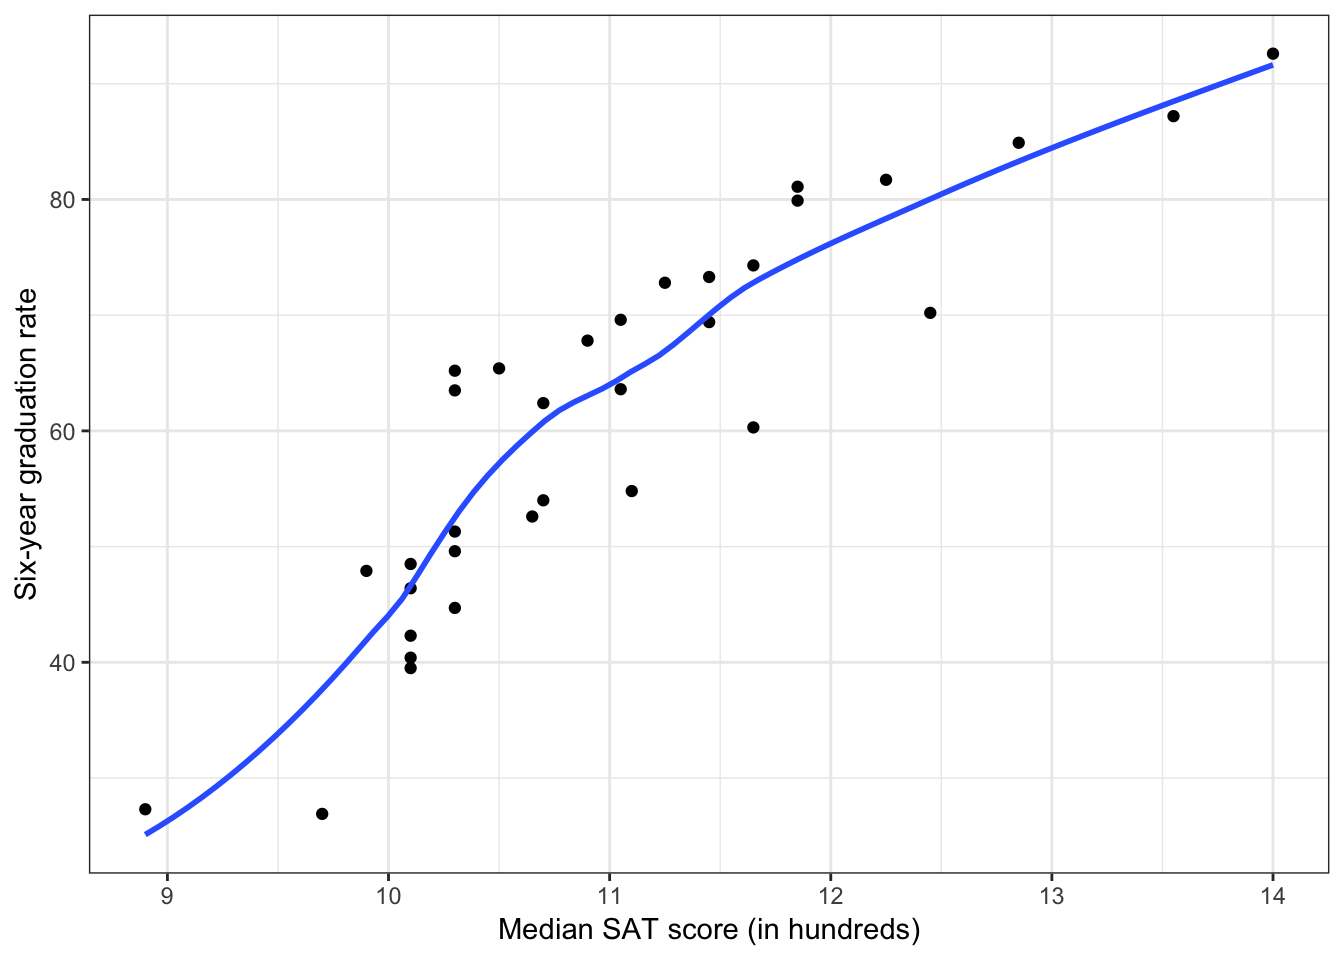
\includegraphics[width=0.5\linewidth]{epsy-8252-notes_files/figure-latex/unnamed-chunk-28-1} 

}

\caption{Scatterplot of the relationship between median SAT score and six-year graduation rate. The loess smoother is also displayed.}\label{fig:unnamed-chunk-28}
\end{figure}

One way to model this nonlinearity was to fit a model that included a polynomial effect (quadratic). Another method of modeling nonlinearity is to transform the predictor (or outcome) using a nonlinear transformation. One commonly used nonlinear transformation is the logarithm. Below is a comparison of the quadratic function to the logarithmic function.

\begin{figure}

{\centering 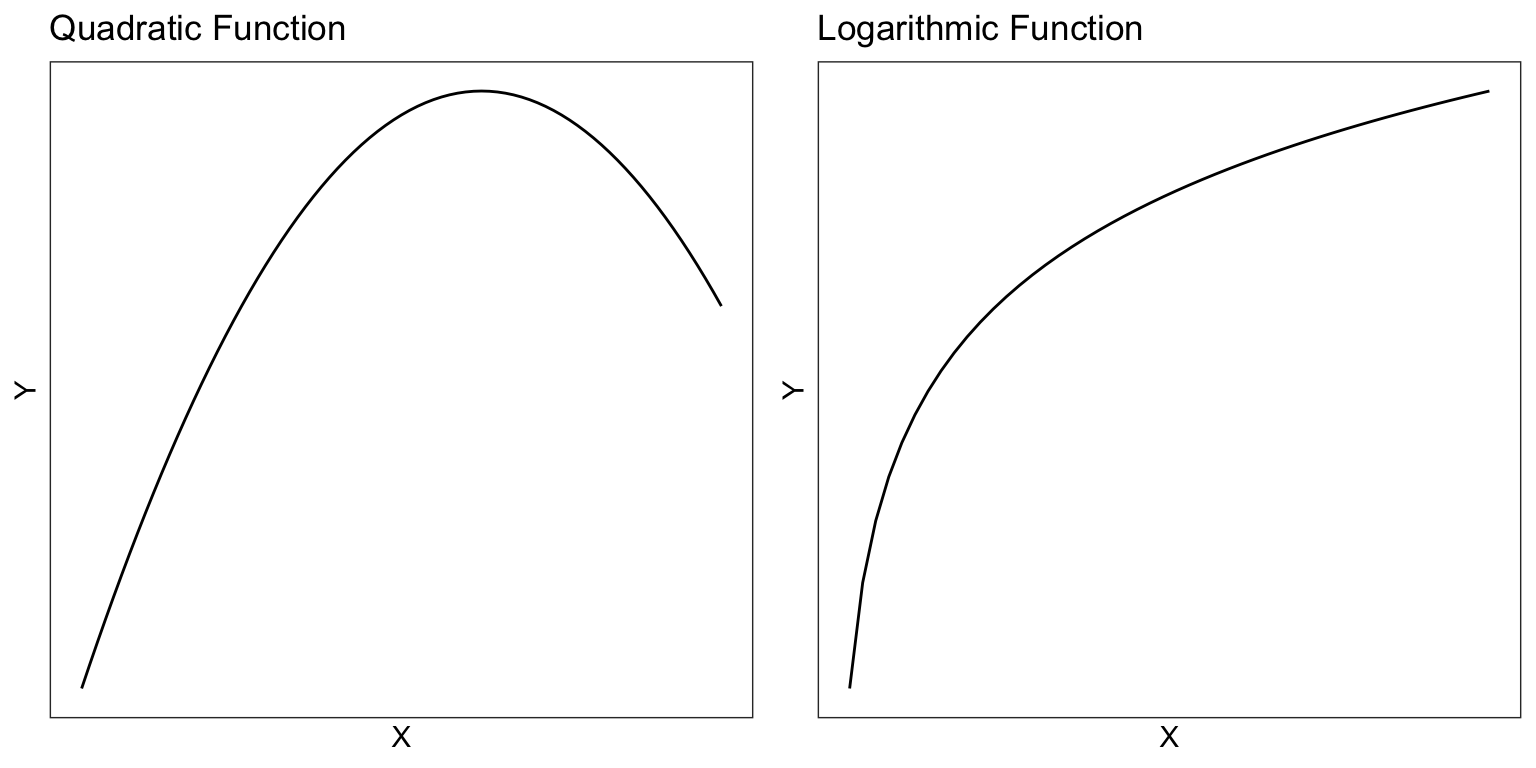
\includegraphics[width=0.8\linewidth]{epsy-8252-notes_files/figure-latex/unnamed-chunk-29-1} 

}

\caption{Quadratic and logarithmic functions.}\label{fig:unnamed-chunk-29}
\end{figure}

The quadratic function shows continuous and diminishing growth followed by continuous and increasing loss (parabola; the function changes direction), while the logarithmic function models continuous, albeit diminishing, growth (the function does not change direction).

\hypertarget{quick-refresher-on-logarithms}{%
\subsection{Quick Refresher on Logarithms}\label{quick-refresher-on-logarithms}}

The logarithm is an inverse function of an exponent. Consider this example,

\[
\log_2 (32)
\]

The logarithm of 32 is the exponent to which the base, 2 in our example, must be raised to produce that number. In other words,

\[
\log_2 (32) \longrightarrow 2^{x} = 32 \longrightarrow x=5
\]

Thus,

\[
\log_2 (32) = 5
\]

To compute a logarithm using R, we use the \texttt{log()} function. We also specify the argument \texttt{base=}, since logarithms are unique to a particular base. For example, to compute the mathematical expression \(\log_2 (32)\), we use

\begin{Shaded}
\begin{Highlighting}[]
\KeywordTok{log}\NormalTok{(}\DecValTok{32}\NormalTok{, }\DataTypeTok{base =} \DecValTok{2}\NormalTok{)}
\end{Highlighting}
\end{Shaded}

\begin{verbatim}
[1] 5
\end{verbatim}

There is also a shortcut function to use base-2.

\begin{Shaded}
\begin{Highlighting}[]
\KeywordTok{log2}\NormalTok{(}\DecValTok{32}\NormalTok{)}
\end{Highlighting}
\end{Shaded}

\begin{verbatim}
[1] 5
\end{verbatim}

\hypertarget{log-transforming-variables}{%
\subsection{Log-Transforming Variables}\label{log-transforming-variables}}

For our purposes, we need to log-transform each value in a particular variable. Here, we will log-transform the SAT variable (using base-2).

\begin{Shaded}
\begin{Highlighting}[]
\NormalTok{mn =}\StringTok{ }\NormalTok{mn }\OperatorTok\StringTok{ }
\StringTok{  }\KeywordTok{mutate}\NormalTok{(}
    \DataTypeTok{L2sat =} \KeywordTok{log}\NormalTok{(sat, }\DataTypeTok{base =} \DecValTok{2}\NormalTok{)}
\NormalTok{    )}

\KeywordTok{head}\NormalTok{(mn)}
\end{Highlighting}
\end{Shaded}

\begin{verbatim}
# A tibble: 6 x 7
     id name                               grad public   sat tuition L2sat
  <dbl> <chr>                             <dbl>  <dbl> <dbl>   <dbl> <dbl>
1     1 Augsburg College                   65.2      0  10.3    39.3  3.36
2     3 Bethany Lutheran College           52.6      0  10.6    30.5  3.41
3     4 Bethel University, Saint Paul, MN  73.3      0  11.4    39.4  3.52
4     5 Carleton College                   92.6      0  14      54.3  3.81
5     6 College of Saint Benedict          81.1      0  11.8    43.2  3.57
6     7 Concordia College at Moorhead      69.4      0  11.4    36.6  3.52
\end{verbatim}

How does this log-transformed variable compare to the original SAT predictor. We can examine the density plot of both the original and log-transformed variables to answer this.

\begin{center}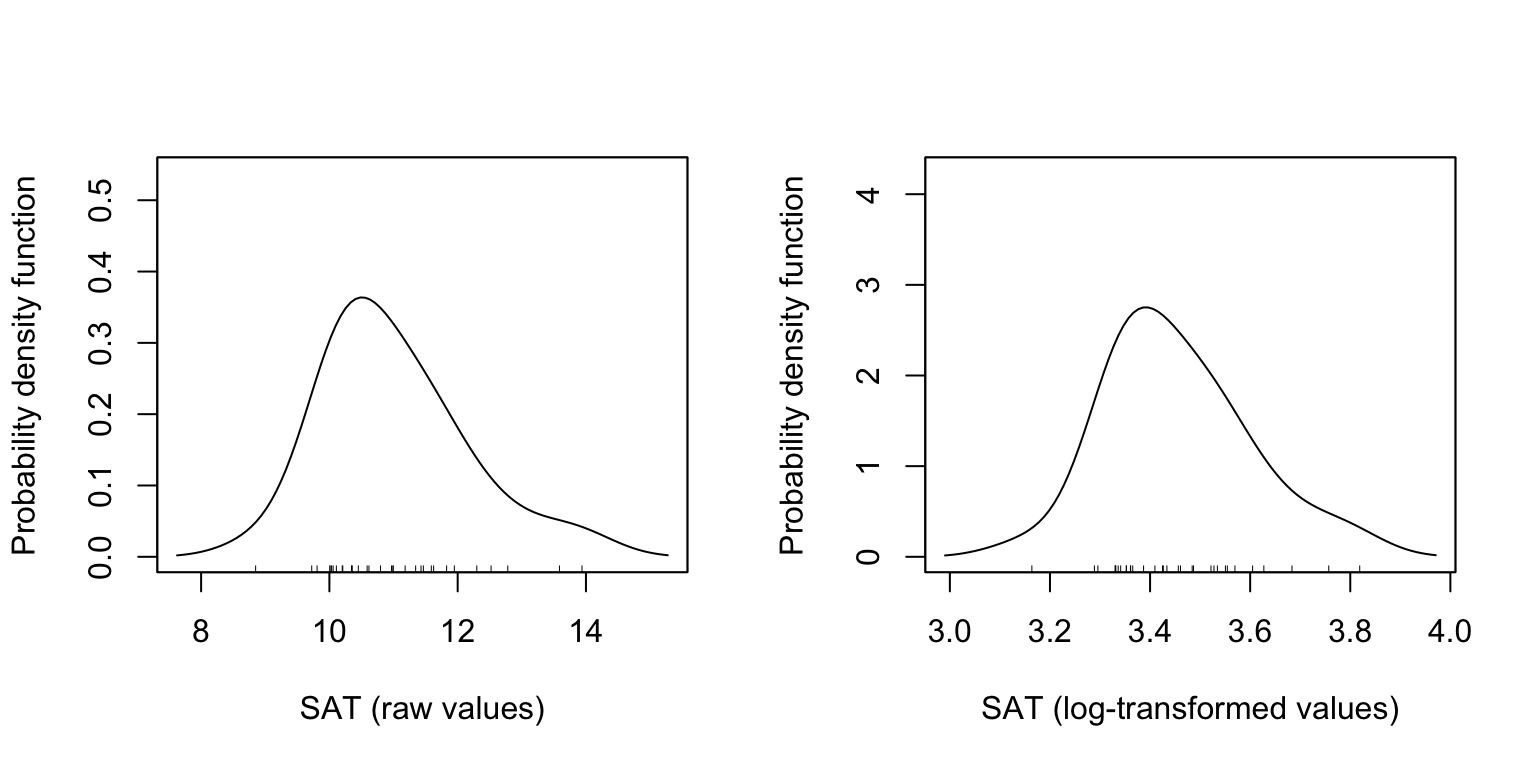
\includegraphics[width=6in]{epsy-8252-notes_files/figure-latex/unnamed-chunk-33-1} \end{center}

\begin{itemize}
\tightlist
\item
  Comparing the shapes of the two variables, we see that the original variable was right-skewed. The log-transformed variable is also right-skewed, although it is LESS right-skewed than the original.
\item
  The scale is quite different between the two variables (one is, after all, log-transformed). This has greatly affected the variation. After log-transforming, the variation is much smaller.
\end{itemize}

What happens when we use the log-transformed variable in a scatterplot with graduation rates?

\begin{Shaded}
\begin{Highlighting}[]
\KeywordTok{ggplot}\NormalTok{(}\DataTypeTok{data =}\NormalTok{ mn, }\KeywordTok{aes}\NormalTok{(}\DataTypeTok{x =}\NormalTok{ L2sat, }\DataTypeTok{y =}\NormalTok{ grad)) }\OperatorTok{+}
\StringTok{  }\KeywordTok{geom_point}\NormalTok{() }\OperatorTok{+}
\StringTok{  }\KeywordTok{geom_smooth}\NormalTok{(}\DataTypeTok{se =} \OtherTok{FALSE}\NormalTok{) }\OperatorTok{+}
\StringTok{  }\KeywordTok{theme_bw}\NormalTok{() }\OperatorTok{+}
\StringTok{  }\KeywordTok{xlab}\NormalTok{(}\StringTok{"Log-transformed SAT score"}\NormalTok{) }\OperatorTok{+}
\StringTok{  }\KeywordTok{ylab}\NormalTok{(}\StringTok{"Six-year graduation rate"}\NormalTok{)}
\end{Highlighting}
\end{Shaded}

\begin{figure}

{\centering 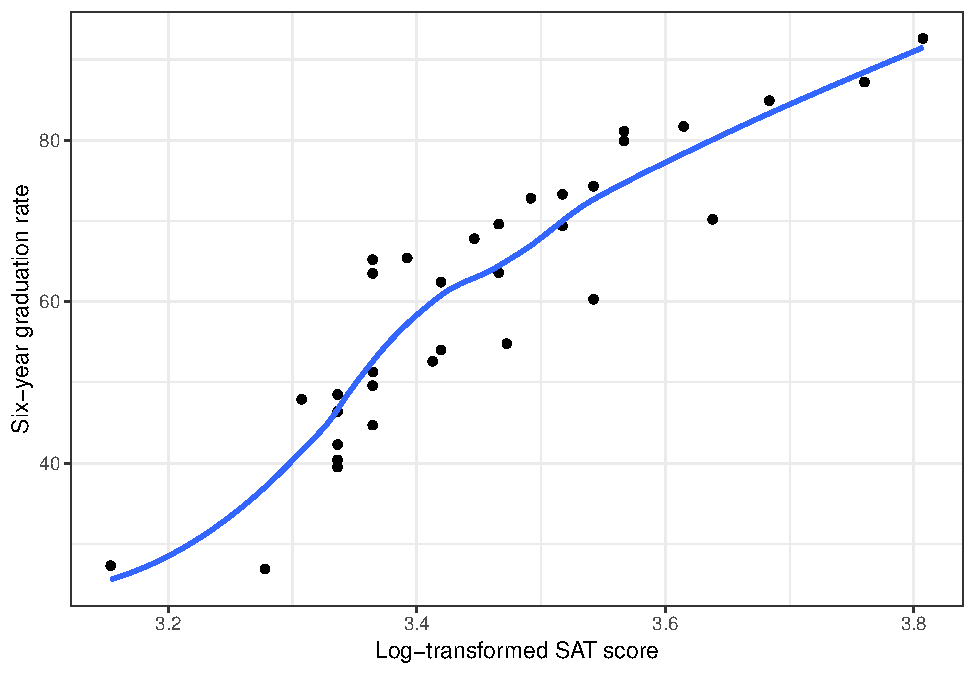
\includegraphics[width=0.5\linewidth]{epsy-8252-notes_files/figure-latex/unnamed-chunk-34-1} 

}

\caption{Scatterplot of the relationship between log-transformed median SAT score (base-2) and six-year graduation rate. The loess smoother is also displayed.}\label{fig:unnamed-chunk-34}
\end{figure}

The relationship between graduation rate and the log-transformed SAT scores is MORE linear than the relationship between graduation rates and the untransformed SAT scores. By transforming the variable using a nonlinear transformation (log) we have ``linearized'' the relationship with graduation rates. As such, we can fit a linear model to predict graduation rates using the Log-transformed SAT scores as a predictor.

\hypertarget{fitting-the-regression-model}{%
\section{Fitting the Regression Model}\label{fitting-the-regression-model}}

To fit the model, we use the \texttt{lm()} function and input the log-transformed SAT scores as the predictor.

\begin{Shaded}
\begin{Highlighting}[]
\NormalTok{lm}\FloatTok{.1}\NormalTok{ =}\StringTok{ }\KeywordTok{lm}\NormalTok{(grad }\OperatorTok{~}\StringTok{ }\DecValTok{1} \OperatorTok{+}\StringTok{ }\NormalTok{L2sat, }\DataTypeTok{data =}\NormalTok{ mn)}
\end{Highlighting}
\end{Shaded}

\hypertarget{examine-the-assumption-of-linearity}{%
\subsection{Examine the Assumption of Linearity}\label{examine-the-assumption-of-linearity}}

Before examining the coefficients, we can scrutinize the residuals to see whether the log-transformation helped us meet the assumption of linearity.

\begin{Shaded}
\begin{Highlighting}[]
\CommentTok{# Obtain residuals}
\NormalTok{out =}\StringTok{ }\KeywordTok{augment}\NormalTok{(lm}\FloatTok{.1}\NormalTok{)}

\CommentTok{# Check linearity assumptions}
\KeywordTok{ggplot}\NormalTok{(}\DataTypeTok{data =}\NormalTok{ out, }\KeywordTok{aes}\NormalTok{(}\DataTypeTok{x =}\NormalTok{ .fitted, }\DataTypeTok{y =}\NormalTok{ .std.resid)) }\OperatorTok{+}
\StringTok{  }\KeywordTok{geom_point}\NormalTok{() }\OperatorTok{+}
\StringTok{  }\KeywordTok{geom_hline}\NormalTok{(}\DataTypeTok{yintercept =} \DecValTok{0}\NormalTok{) }\OperatorTok{+}
\StringTok{  }\KeywordTok{geom_smooth}\NormalTok{() }\OperatorTok{+}
\StringTok{  }\KeywordTok{theme_bw}\NormalTok{()}
\end{Highlighting}
\end{Shaded}

\begin{center}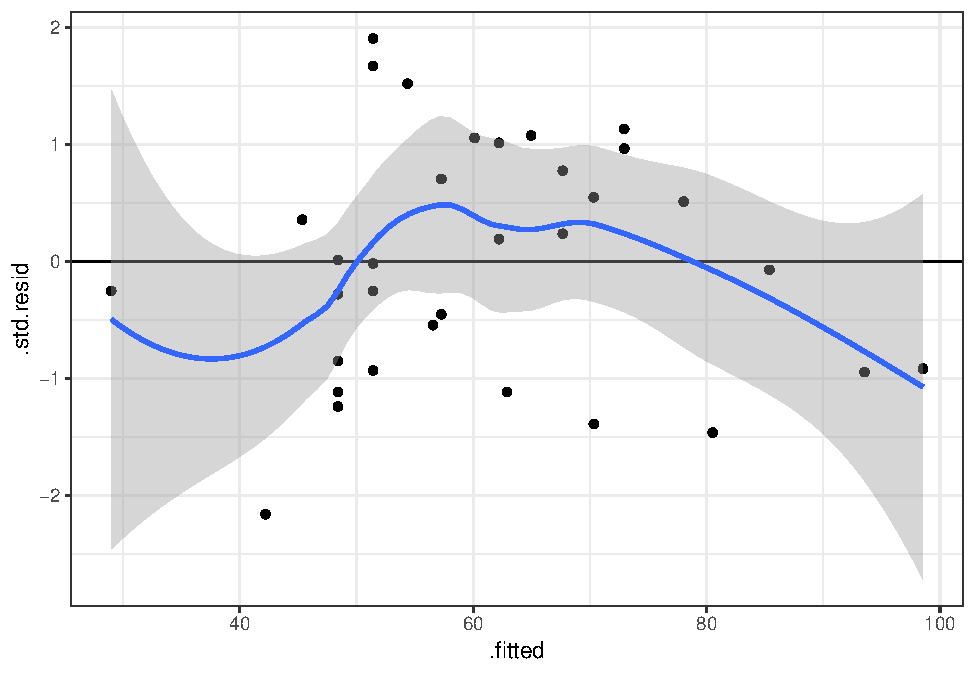
\includegraphics[width=3.5in]{epsy-8252-notes_files/figure-latex/unnamed-chunk-36-1} \end{center}

The assumption looks reasonably met as the horizontal line of \(y=0\) is encompassed in the confidence envelope of the loess smoother.

\hypertarget{interpret-the-regression-results}{%
\subsection{Interpret the Regression Results}\label{interpret-the-regression-results}}

We can now look at the regression output and interpret the results.

\begin{Shaded}
\begin{Highlighting}[]
\CommentTok{# Model-level output}
\KeywordTok{glance}\NormalTok{(lm}\FloatTok{.1}\NormalTok{)}
\end{Highlighting}
\end{Shaded}

\begin{verbatim}
# A tibble: 1 x 11
  r.squared adj.r.squared sigma statistic  p.value    df logLik   AIC   BIC
      <dbl>         <dbl> <dbl>     <dbl>    <dbl> <int>  <dbl> <dbl> <dbl>
1     0.811         0.805  7.39      133. 9.30e-13     2  -112.  230.  234.
# ... with 2 more variables: deviance <dbl>, df.residual <int>
\end{verbatim}

Examining the model-level output, we see that differences in \(\log_2(\mathrm{SAT})\) explain 81.13\% of the variation in graduation rates. This is statistically significant, \(F(1,~31)=133.3\), \(p<.001\). Since differences in \(\log_2(\mathrm{SAT})\) imply that there are differences in the raw SAT scores, we would typically just say that ``differences in SAT scores explain 81.13\% of the variation in graduation rates.''

Moving to the coefficient-level output,

\begin{Shaded}
\begin{Highlighting}[]
\CommentTok{# Coefficient-level output}
\KeywordTok{tidy}\NormalTok{(lm}\FloatTok{.1}\NormalTok{)}
\end{Highlighting}
\end{Shaded}

\begin{verbatim}
# A tibble: 2 x 5
  term        estimate std.error statistic  p.value
  <chr>          <dbl>     <dbl>     <dbl>    <dbl>
1 (Intercept)    -307.     31.9      -9.62 7.94e-11
2 L2sat           106.      9.22     11.5  9.30e-13
\end{verbatim}

We can write the fitted equation as,

\[
\hat{\mathrm{Graduation~Rate}} = -306.7 + 106.4\bigg[\log_2(\mathrm{SAT})\bigg]
\]

We can interpret the coefficients as we always do, recognizing that these interpretation are based on the log-transformed predictor.

\begin{itemize}
\tightlist
\item
  The intercept value of \(-306.7\) is the predicted average graduation rate for all colleges/universities with a \(\log_2(\mathrm{SAT})\) value of 0.
\item
  The slope value of 106.4 indicates that each one-unit difference in \(\log_2(\mathrm{SAT})\) is associated with a 106.4-unit difference in graduation rate, on average.
\end{itemize}

\hypertarget{better-interpretations-back-transforming}{%
\subsection{Better Interpretations: Back-transforming}\label{better-interpretations-back-transforming}}

While these interpretations are technically correct, it is more helpful to your readers (and more conventional) to interpret any regression results in the metric of SAT scores rather than log-transformed SAT scores. This means we have to \emph{back-transform the interpretations}. To back-transform a logarithm, we use its inverse function; exponentiation.

We interpreted the intercept as, ``the predicted average graduation rate for all colleges/universities with a \(\log_2(\mathrm{SAT})\) value of 0''. To interpret this using the metric of our SAT attribute, we have to understand what \(\log_2(\mathrm{SAT}) = 0\) is.

\[
\log_2 (\mathrm{SAT}) = 0 \longrightarrow 2^{0} = \mathrm{SAT}
\]

In this computation, \(\mathrm{SAT}=1\). Thus, rather than using the log-transformed interpretation, we can, instead, interpret the intercept as,

\begin{quote}
The predicted average graduation rate for all colleges/universities with a SAT measurement of 1 (median SAT = 100) is \(-306.7\). Since there are no colleges/universities in our data that have a SAT value of 1, this is extrapolation.
\end{quote}

What about the slope? Our interpretation was that ``each one-unit difference in \(\log_2(\mathrm{SAT})\) is associated with a 106.4-unit difference in graduation rate, on average.'' Working with the same ideas of back-transformation, we need to understand what a one-unit difference in \(\log_2(\mathrm{SAT})\) means. Consider four values of \(\log_2(\mathrm{SAT})\) that are each one-unit apart:

\[
\log_2(\mathrm{SAT}) = 1\\
\log_2(\mathrm{SAT}) = 2\\
\log_2(\mathrm{SAT}) = 3\\
\log_2(\mathrm{SAT}) = 4
\]

If we back-transform each of these, then we can see how the four values of the raw SAT variable would differ.

\[
\begin{split}
\mathrm{SAT} &= 2^1 = 2\\
\mathrm{SAT} &= 2^2 = 4\\
\mathrm{SAT} &= 2^3 = 8\\
\mathrm{SAT} &= 2^4 = 16
\end{split}
\]

When \(\log_2(\mathrm{SAT})\) is increased by one-unit, the raw SAT value is doubled. We can use this in our interpretation of slope:

\begin{quote}
A doubling of the SAT value is associated with a 106.4-unit difference in graduation rate, on average.
\end{quote}

The technical language for doubling is a ``two-fold difference''. So we would conventionally interpret this as:

\begin{quote}
Each two-fold difference in SAT value is associated with a 106.4-unit difference in graduation rate, on average.
\end{quote}

To understand this further, consider a specific school, say Augsburg. Their measurement on the SAT variable is 10.3, and their log-transformed SAT score is 3.36. Using the fitted regression equation (which employs the log-transformed SAT),

\begin{Shaded}
\begin{Highlighting}[]
\FloatTok{-306.7} \OperatorTok{+}\StringTok{ }\FloatTok{106.4} \OperatorTok{*}\StringTok{ }\FloatTok{3.36}
\end{Highlighting}
\end{Shaded}

\begin{verbatim}
[1] 50.8
\end{verbatim}

Augsburg's predicted graduation rate would be 50.8. If we increase the \texttt{L2sat} score by 1 to 4.36 (which is equivalent to a raw SAT measurement of 20.6; double 10.3), their predicted graduation rate is,

\begin{Shaded}
\begin{Highlighting}[]
\FloatTok{-306.7} \OperatorTok{+}\StringTok{ }\FloatTok{106.4} \OperatorTok{*}\StringTok{ }\FloatTok{4.36}
\end{Highlighting}
\end{Shaded}

\begin{verbatim}
[1] 157.2
\end{verbatim}

This is an increase of 106.4.

\hypertarget{alternative-method-of-fitting-the-model}{%
\section{Alternative Method of Fitting the Model}\label{alternative-method-of-fitting-the-model}}

Rather that create the log-transformed SAT score in the data, we can use the \texttt{log()} function on SAT directly in the \texttt{lm()} computation.

\begin{Shaded}
\begin{Highlighting}[]
\NormalTok{lm}\FloatTok{.1}\NormalTok{ =}\StringTok{ }\KeywordTok{lm}\NormalTok{(grad }\OperatorTok{~}\StringTok{ }\DecValTok{1} \OperatorTok{+}\StringTok{ }\KeywordTok{log}\NormalTok{(sat, }\DataTypeTok{base =} \DecValTok{2}\NormalTok{), }\DataTypeTok{data =}\NormalTok{ mn)}

\CommentTok{# Model-level output}
\KeywordTok{glance}\NormalTok{(lm}\FloatTok{.1}\NormalTok{)}
\end{Highlighting}
\end{Shaded}

\begin{verbatim}
# A tibble: 1 x 11
  r.squared adj.r.squared sigma statistic  p.value    df logLik   AIC   BIC
      <dbl>         <dbl> <dbl>     <dbl>    <dbl> <int>  <dbl> <dbl> <dbl>
1     0.811         0.805  7.39      133. 9.30e-13     2  -112.  230.  234.
# ... with 2 more variables: deviance <dbl>, df.residual <int>
\end{verbatim}

\begin{Shaded}
\begin{Highlighting}[]
\CommentTok{# Coefficient-level output}
\KeywordTok{tidy}\NormalTok{(lm}\FloatTok{.1}\NormalTok{)}
\end{Highlighting}
\end{Shaded}

\begin{verbatim}
# A tibble: 2 x 5
  term               estimate std.error statistic  p.value
  <chr>                 <dbl>     <dbl>     <dbl>    <dbl>
1 (Intercept)           -307.     31.9      -9.62 7.94e-11
2 log(sat, base = 2)     106.      9.22     11.5  9.30e-13
\end{verbatim}

Using this method of fitting the model will be useful as we plot the fitted model.

\hypertarget{plotting-the-fitted-model}{%
\section{Plotting the Fitted Model}\label{plotting-the-fitted-model}}

To aid interpretation of the effect of SAT on graduation rate, we can plot the fitted model. If we used the method of fitting in which we used \texttt{log()} directly in the \texttt{lm()} function, we only need to set up a sequence of SAT values, predict graduation rates using the fitted model, and finally connect these values using a line.

\begin{Shaded}
\begin{Highlighting}[]
\CommentTok{# Set up data}
\NormalTok{plot_data =}\StringTok{ }\KeywordTok{crossing}\NormalTok{(}
    \DataTypeTok{sat =} \KeywordTok{seq}\NormalTok{(}\DataTypeTok{from =} \FloatTok{8.9}\NormalTok{, }\DataTypeTok{to =} \FloatTok{14.0}\NormalTok{, }\DataTypeTok{by =} \FloatTok{0.1}\NormalTok{)}
\NormalTok{    ) }\OperatorTok
\StringTok{  }\KeywordTok{mutate}\NormalTok{(}
    \CommentTok{# Predict}
    \DataTypeTok{yhat =} \KeywordTok{predict}\NormalTok{(lm}\FloatTok{.1}\NormalTok{, }\DataTypeTok{newdata =}\NormalTok{ .)}
\NormalTok{  )}

\CommentTok{# Examine data}
\KeywordTok{head}\NormalTok{(plot_data)}
\end{Highlighting}
\end{Shaded}

\begin{verbatim}
# A tibble: 6 x 2
    sat  yhat
  <dbl> <dbl>
1   8.9  29.0
2   9    30.7
3   9.1  32.4
4   9.2  34.1
5   9.3  35.7
6   9.4  37.4
\end{verbatim}

\begin{Shaded}
\begin{Highlighting}[]
\CommentTok{# Plot}
\KeywordTok{ggplot}\NormalTok{(}\DataTypeTok{data =}\NormalTok{ plot_data, }\KeywordTok{aes}\NormalTok{(}\DataTypeTok{x =}\NormalTok{ sat, }\DataTypeTok{y =}\NormalTok{ yhat)) }\OperatorTok{+}
\StringTok{    }\KeywordTok{geom_line}\NormalTok{() }\OperatorTok{+}
\StringTok{    }\KeywordTok{theme_bw}\NormalTok{() }\OperatorTok{+}
\StringTok{  }\KeywordTok{xlab}\NormalTok{(}\StringTok{"Median SAT score (in hundreds)"}\NormalTok{) }\OperatorTok{+}
\StringTok{  }\KeywordTok{ylab}\NormalTok{(}\StringTok{"Predicted graduation rate"}\NormalTok{)}
\end{Highlighting}
\end{Shaded}

\begin{figure}

{\centering 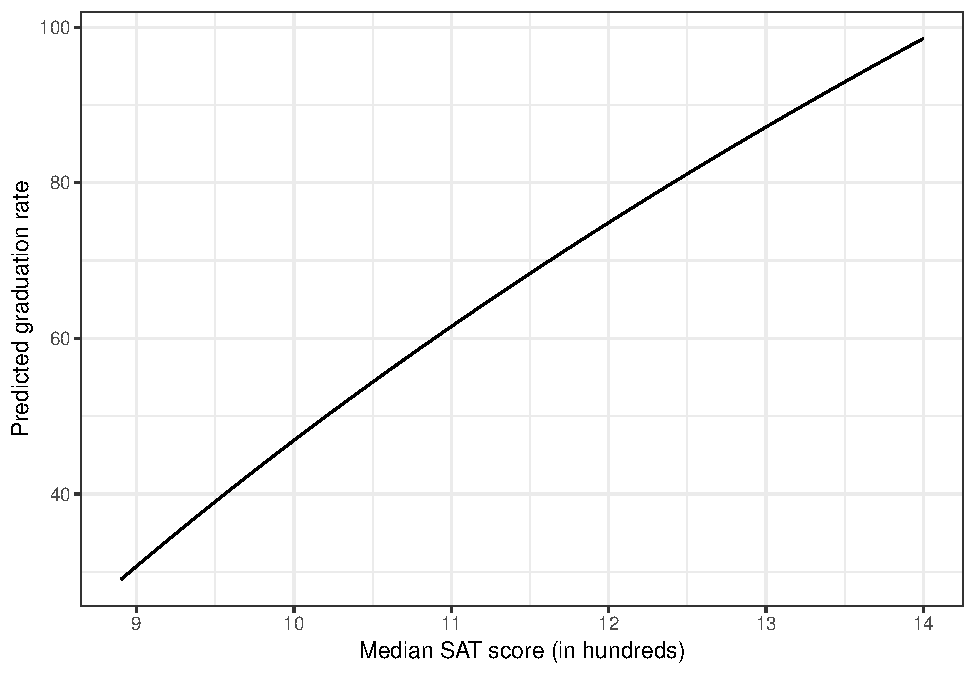
\includegraphics[width=0.5\linewidth]{epsy-8252-notes_files/figure-latex/unnamed-chunk-42-1} 

}

\caption{Plot of the predicted graduation rates as a function of median SAT score (in hundreds). The non-linearity in the plot indicates that there is a diminishing positive effect of SAT on graduation rates.}\label{fig:unnamed-chunk-42}
\end{figure}

\hypertarget{different-base-values-in-the-logarithm}{%
\section{Different Base Values in the Logarithm}\label{different-base-values-in-the-logarithm}}

The base value we used in the \texttt{log()} function in the previous example was base-2. Using a base value of 2 was an arbitrary choice. We can use any base value we want. For example, what happens if we use base-10.

\begin{Shaded}
\begin{Highlighting}[]
\NormalTok{mn =}\StringTok{ }\NormalTok{mn }\OperatorTok
\StringTok{  }\KeywordTok{mutate}\NormalTok{(}
    \DataTypeTok{L10sat =} \KeywordTok{log}\NormalTok{(mn}\OperatorTok{$}\NormalTok{sat, }\DataTypeTok{base =} \DecValTok{10}\NormalTok{)}
\NormalTok{  )}

\CommentTok{# Examine data}
\KeywordTok{head}\NormalTok{(mn)}
\end{Highlighting}
\end{Shaded}

\begin{verbatim}
# A tibble: 6 x 8
     id name                         grad public   sat tuition L2sat L10sat
  <dbl> <chr>                       <dbl>  <dbl> <dbl>   <dbl> <dbl>  <dbl>
1     1 Augsburg College             65.2      0  10.3    39.3  3.36   1.01
2     3 Bethany Lutheran College     52.6      0  10.6    30.5  3.41   1.03
3     4 Bethel University, Saint P~  73.3      0  11.4    39.4  3.52   1.06
4     5 Carleton College             92.6      0  14      54.3  3.81   1.15
5     6 College of Saint Benedict    81.1      0  11.8    43.2  3.57   1.07
6     7 Concordia College at Moorh~  69.4      0  11.4    36.6  3.52   1.06
\end{verbatim}

Comparing the logarithms of the SAT attribute using base-10 to those using base-2 we see that the base-10 logarithms are smaller. This is because now we are using the base of 10 in our exponent (rather than 2). For example, for Augsburg,

\[
10^{1.013} = 10.3
\]

If we fit a model using the base-10 logarithm,

\begin{Shaded}
\begin{Highlighting}[]
\NormalTok{lm}\FloatTok{.2}\NormalTok{ =}\StringTok{ }\KeywordTok{lm}\NormalTok{(grad }\OperatorTok{~}\StringTok{ }\DecValTok{1} \OperatorTok{+}\StringTok{ }\KeywordTok{log}\NormalTok{(sat, }\DataTypeTok{base =} \DecValTok{10}\NormalTok{), }\DataTypeTok{data =}\NormalTok{ mn)}

\CommentTok{# Model-level output}
\KeywordTok{glance}\NormalTok{(lm}\FloatTok{.2}\NormalTok{)}
\end{Highlighting}
\end{Shaded}

\begin{verbatim}
# A tibble: 1 x 11
  r.squared adj.r.squared sigma statistic  p.value    df logLik   AIC   BIC
      <dbl>         <dbl> <dbl>     <dbl>    <dbl> <int>  <dbl> <dbl> <dbl>
1     0.811         0.805  7.39      133. 9.30e-13     2  -112.  230.  234.
# ... with 2 more variables: deviance <dbl>, df.residual <int>
\end{verbatim}

Examining the model-level output, we see that differences in \(\log_{10}(\mathrm{SAT})\) explain 81.13\% of the variation in graduation rates. Or simply, that differences in SAT scores explain 81.13\% of the variation in graduation rates. This is statistically significant, \(F(1,~31)=133.3\), \(p<.001\). These model-level results are the same as when we used the base-2 logarithm.

\begin{Shaded}
\begin{Highlighting}[]
\CommentTok{# Coefficient-level output}
\KeywordTok{tidy}\NormalTok{(lm}\FloatTok{.2}\NormalTok{)}
\end{Highlighting}
\end{Shaded}

\begin{verbatim}
# A tibble: 2 x 5
  term                estimate std.error statistic  p.value
  <chr>                  <dbl>     <dbl>     <dbl>    <dbl>
1 (Intercept)            -307.      31.9     -9.62 7.94e-11
2 log(sat, base = 10)     354.      30.6     11.5  9.30e-13
\end{verbatim}

The fitted equation is,

\[
\hat{\mathrm{Graduation~Rate}} = -306.7 + 353.6\bigg[\log_{10}(\mathrm{SAT})\bigg]
\]

We can interpret the coefficients using the base-10 logarithm of SAT scores as:

\begin{itemize}
\tightlist
\item
  The intercept value of \(-306.7\) is the predicted average graduation rate for all colleges/universities with a \(\log_{10}(\mathrm{SAT})\) value of 0.
\item
  The slope value of 353.6 indicates that each one-unit difference in \(\log_{10}(\mathrm{SAT})\) is associated with a 353.6-unit difference in graduation rate, on average.
\end{itemize}

Better yet, we can \emph{back-transform the interpretations} so that we are using SAT scores rather than \(\log_{10}(\mathrm{SAT})\) scores.

\begin{itemize}
\tightlist
\item
  The predicted average graduation rate for all colleges/universities with a SAT value of 1 (median SAT score = 100) is \(-306.7\).
\item
  Each \emph{ten-fold} difference in SAT is associated with a 353.6-unit difference in graduation rate, on average.
\end{itemize}

To further think about the effect of SAT, if Augsburg improved its median SAT score ten-fold (i.e., going from a SAT value of 10.3 to a value of 103) we would predict its graduation rate to go up by 353.6.

\hypertarget{comparing-the-output-from-the-two-bases}{%
\subsection{Comparing the Output from the Two Bases}\label{comparing-the-output-from-the-two-bases}}

The model-level information is all the same. Furthermore, the intercepts (and SE and \(p\)-value) was the same across both models. The slope coefficients and SEs were different in the two models, but the \(t\)-value and \(p\)-value for the effect of SAT was identical for both base-2 and base-10. The only real difference in using base-10 vs.~base-2 in the logarithm is in the interpretation of the SAT effect.

What if we look at the residual fit?

\begin{figure}

{\centering 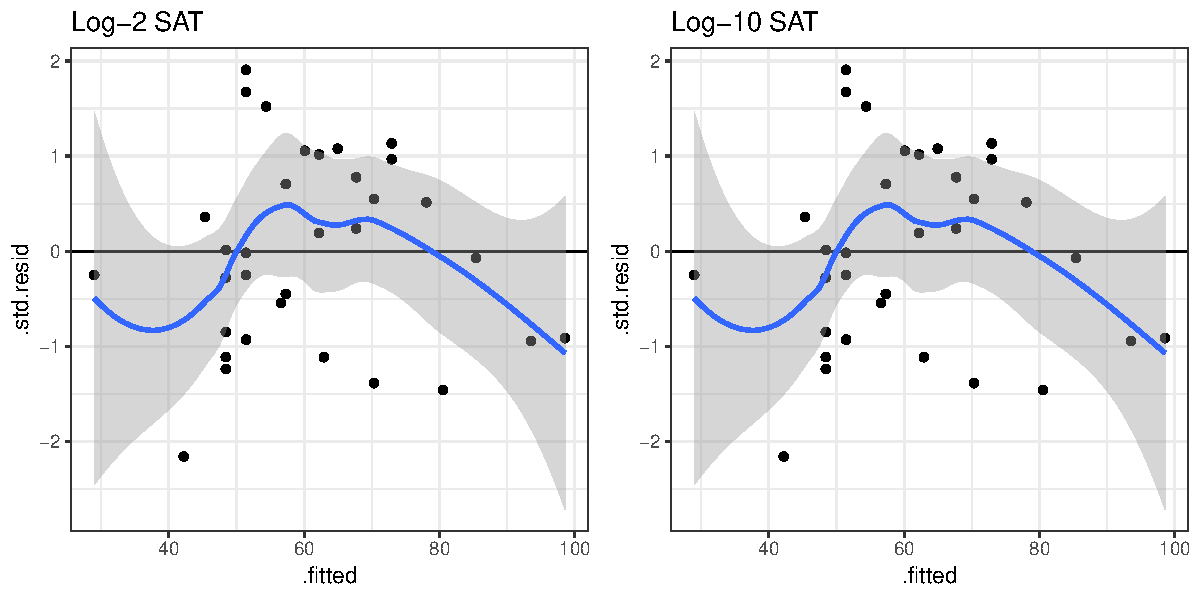
\includegraphics[width=0.8\linewidth]{epsy-8252-notes_files/figure-latex/unnamed-chunk-46-1} 

}

\caption{Standardized residuals versus the fitted values for the models fitted with the log-2 predictor (left) and the log-10 predictor (right).}\label{fig:unnamed-chunk-46}
\end{figure}

\newpage

The residuals fit EXACTLY the same. Why is this? Let's again use Augsburg as an example. Using the fitted model that employed the base-2 logarithm, we found that Augsburg's predicted graduation rate was,

\[
\begin{split}
\hat{\mathrm{Graduation~Rate}} &= -306.7 + 106.4\bigg[\log_2(10.3)\bigg] \\
&= -306.7 + 106.4\bigg[3.36\bigg] \\
&= 50.8
\end{split}
\]

Using the model that employed the base-10 logarithm, Augsburg's predicted graduation rate would be

\[
\begin{split}
\hat{\mathrm{Graduation~Rate}} &= -306.7 + 353.6\bigg[\log_{10}(10.3)\bigg] \\
&= -306.7 + 353.6\bigg[1.01\bigg] \\
&= 50.8
\end{split}
\]

Augsburg's predicted graduation rate is \emph{exactly the same} in the two models. This implies that Augsburg's residual would also be the same in the two models. This is true for every college. Because of this, increasing (or decreasing) the base used in the logarithm does not help improve the fit of the model. The fit is exactly the same no matter which base you choose.

The only thing that changes when you choose a different base is the interpretation of the slope. You should choose the base to facilitate interpretation. For example, does it make more sense to talk about a \emph{two-fold} difference in the predictor? A \emph{five-fold} difference in the predictor? A \emph{ten-fold} difference in the predictor?

\hypertarget{base-e-logarithm-the-natural-logarithm}{%
\section{\texorpdfstring{Base-\(e\) Logarithm: The Natural Logarithm}{Base-e Logarithm: The Natural Logarithm}}\label{base-e-logarithm-the-natural-logarithm}}

In our example, neither of the bases we examined is satisfactory in terms of talking about the effect of SAT. Two-fold differences in SAT are very unlikely, to say anything of ten-fold differences. One base that is commonly used for log-transformations is base-\(e\). \(e\) is a mathematical constant (Euler's number) that is approximately equal to 2.71828. We can obtain this by using the \texttt{exp()} function in R. This function takes \(e\) to some exponent that is given as the argument. So to obtain the approximation of \(e\) we use

\begin{Shaded}
\begin{Highlighting}[]
\KeywordTok{exp}\NormalTok{(}\DecValTok{1}\NormalTok{)}
\end{Highlighting}
\end{Shaded}

\begin{verbatim}
[1] 2.718
\end{verbatim}

The logarithm (base-\(e\)) for a number, referred to as the \emph{natural logarithm}, can be obtained using the \texttt{log()} function with the argument \texttt{base=exp(1)}. However, this base is so commonly used that it is the default value for the \texttt{base=} argument. So, if we use the \texttt{log()} function without defining the \texttt{base=} argument, it will automatically use base-\(e\). For example, the natural logarithm of Augsburg's SAT score of 1030 can be computed as

\begin{Shaded}
\begin{Highlighting}[]
\KeywordTok{log}\NormalTok{(}\FloatTok{10.3}\NormalTok{)}
\end{Highlighting}
\end{Shaded}

\begin{verbatim}
[1] 2.332
\end{verbatim}

If we took \(e^{2.332}\) we would obtain 10.3. The natural logarithm even has its own mathematical notation; \(\ln\). For example, we would mathematically express the natural logarithm of 10.3 as

\[
\ln (10.3) = 2.332.
\]

\hypertarget{using-the-natural-logarithm-in-a-regression-model}{%
\subsection{Using the Natural Logarithm in a Regression Model}\label{using-the-natural-logarithm-in-a-regression-model}}

Below we regress graduation rates on the log-transformed SAT scores, using the natural logarithm.

\begin{Shaded}
\begin{Highlighting}[]
\CommentTok{# Fit model}
\NormalTok{lm}\FloatTok{.3}\NormalTok{ =}\StringTok{ }\KeywordTok{lm}\NormalTok{(grad }\OperatorTok{~}\StringTok{ }\DecValTok{1} \OperatorTok{+}\StringTok{ }\KeywordTok{log}\NormalTok{(sat), }\DataTypeTok{data =}\NormalTok{ mn)}

\CommentTok{# Model-level output}
\KeywordTok{glance}\NormalTok{(lm}\FloatTok{.3}\NormalTok{)}
\end{Highlighting}
\end{Shaded}

\begin{verbatim}
# A tibble: 1 x 11
  r.squared adj.r.squared sigma statistic  p.value    df logLik   AIC   BIC
      <dbl>         <dbl> <dbl>     <dbl>    <dbl> <int>  <dbl> <dbl> <dbl>
1     0.811         0.805  7.39      133. 9.30e-13     2  -112.  230.  234.
# ... with 2 more variables: deviance <dbl>, df.residual <int>
\end{verbatim}

As with any base, using base-\(e\) results in the same model-level information (\(R^2=.811\), \(F(1,~31)=133.3\), \(p<.001\)).

\begin{Shaded}
\begin{Highlighting}[]
\CommentTok{# Coefficient-level output}
\KeywordTok{tidy}\NormalTok{(lm}\FloatTok{.3}\NormalTok{)}
\end{Highlighting}
\end{Shaded}

\begin{verbatim}
# A tibble: 2 x 5
  term        estimate std.error statistic  p.value
  <chr>          <dbl>     <dbl>     <dbl>    <dbl>
1 (Intercept)    -307.      31.9     -9.62 7.94e-11
2 log(sat)        154.      13.3     11.5  9.30e-13
\end{verbatim}

The intercept has the same coefficient (\(\hat\beta_0=-306.7\)), SE, \(t\)-value, and \(p\)-value as the intercept from the models using base-2 and base-10 log-transformations of SAT. (This is, again, because \(2^0=10^0=e^0=1\).) And, although the coefficient and SE for the effect of SAT is again different (a one-unit change in the three different log-scales does not correspond to the same amount of change in raw SAT for the three models), the \(t\)-value and level of statistical significance (\(t(31)=11.55\), \(p<.001\)) for this effect, are the same as when we used base-2 and base-10.

So how can we interpret the model's coefficients?

\begin{itemize}
\tightlist
\item
  The intercept can be interpreted exactly the same as in the previous models in which we used base-2 or base-10; namely that the predicted average graduation rate for colleges/universities with a SAT value of one is \(-306.7\).
\item
  Interpreting the slope, we could say that an \(e\)-fold difference in SAT value is associated with a 153.6-unit difference in graduation rates, on average.
\end{itemize}

\hypertarget{interpretation-using-percentage-change}{%
\subsubsection{Interpretation Using Percentage Change}\label{interpretation-using-percentage-change}}

Consider three schools, each having a SAT score that differs by 1\%; say these schools have SAT values of 10, 10.1, 10.2. Using the fitted equation, we can compute the predicted graduation rate for each of these hypothetical schools:

\[
\hat{\mathrm{Graduation~Rate}} = -306.7 + 153.6 \bigg[\ln (\mathrm{SAT})\bigg]
\]

The SAT values and predicted graduation rates for these schools are given below:

\label{tab:unnamed-chunk-51}SAT values and Graduation Rates for Three Hypothetical Schools that have SAT Values that Differ by One Percent.

SAT

Predicted Graduation Rate

10.0

46.88

10.1

48.41

10.2

49.93

The difference between each subsequent predicted graduation rate is 1.53.

\begin{Shaded}
\begin{Highlighting}[]
\FloatTok{48.4058} \OperatorTok{-}\StringTok{ }\FloatTok{46.8778}
\end{Highlighting}
\end{Shaded}

\begin{verbatim}
[1] 1.528
\end{verbatim}

\begin{Shaded}
\begin{Highlighting}[]
\FloatTok{49.9338} \OperatorTok{-}\StringTok{ }\FloatTok{48.4058}
\end{Highlighting}
\end{Shaded}

\begin{verbatim}
[1] 1.528
\end{verbatim}

In other words, schools that have a SAT value that differ by 1\%, have predicted graduation rates that differ by 1.53, on average.

\hypertarget{mathematical-explanation}{%
\subsubsection{Mathematical Explanation}\label{mathematical-explanation}}

To understand how we can directly compute this difference, consider the predicted values for two \(x\)-values that differ by one-percent, if we use symbolic notation:

\[
\begin{split}
\hat{y}_1 &= \hat\beta_0 + \hat\beta_1\left[\ln(x)\right] \\
\hat{y}_2 &= \hat\beta_0 + \hat\beta_1\left[\ln(1.01x)\right]
\end{split}
\]

The difference in their predicted values is:

\[
\begin{split}
\hat{y}_2 - \hat{y}_1 &= \hat\beta_0 + \hat\beta_1\left[\ln(1.01x)\right] - \left(\hat\beta_0 + \hat\beta_1\left[\ln(x)\right]\right) \\
&=\hat\beta_0 + \hat\beta_1\left[\ln(1.01x)\right] - \hat\beta_0 - \hat\beta_1\left[\ln(x)\right] \\
&=\hat\beta_1\left[\ln(1.01x)\right] - \hat\beta_1\left[\ln(x)\right] \\
&=\hat\beta_1\left[\ln(1.01x) - \ln(x)\right]\\
&=\hat\beta_1\left[\ln(\frac{1.01x}{1x})\right]
\end{split}
\]

If we substitute in any value for \(x\), we can now directly compute this constant difference. Note that a convenient value for \(x\) is 1. Then this reduces to:

\[
\hat\beta_1\left[\ln(1.01)\right]
\]

So now, we can interpret this as: a one-percent difference in \(x\) is associated with a \(\hat\beta_1\left[\ln(1.01)\right]\)-unit difference in \(Y\), on average.

In our model, we can compute this difference using the fitted coefficient \(\hat\beta_1=153.6\) as

\[
153.6\left[\ln(1.01)\right] = 1.528371
\]

The same computation using R is

\begin{Shaded}
\begin{Highlighting}[]
\FloatTok{153.6} \OperatorTok{*}\StringTok{ }\KeywordTok{log}\NormalTok{(}\FloatTok{1.01}\NormalTok{)}
\end{Highlighting}
\end{Shaded}

\begin{verbatim}
[1] 1.528
\end{verbatim}

This gives you the constant difference exactly. So you can interpret the effect of SAT as, each 1\% difference in SAT score is associated with a difference in graduation rates of 1.53, on average.

\hypertarget{approximate-interpretation}{%
\subsubsection{Approximate Interpretation}\label{approximate-interpretation}}

We can get an approximate estimate for the size of the effect by using the mathematical shortcut of

\[
\mathrm{Effect} \approx \frac{\hat\beta_1}{100}
\]

Using our fitted results, we could approximate the size of the effect as,

\[
\frac{153.6}{100} = 1.536
\]

We could then interpret the effect of SAT by saying a 1\% difference in median SAT score is associated with a 1.53-unit difference in predicted graduation rate, on average.

\hypertarget{including-covariates}{%
\section{Including Covariates}\label{including-covariates}}

We can also include covariates in the model. Below we examine the nonlinear effect of SAT on graduation controlling for differences in sector.

\begin{Shaded}
\begin{Highlighting}[]
\CommentTok{# Fit model}
\NormalTok{lm}\FloatTok{.4}\NormalTok{ =}\StringTok{ }\KeywordTok{lm}\NormalTok{(grad }\OperatorTok{~}\StringTok{ }\DecValTok{1} \OperatorTok{+}\StringTok{ }\NormalTok{public }\OperatorTok{+}\StringTok{ }\KeywordTok{log}\NormalTok{(sat), }\DataTypeTok{data =}\NormalTok{ mn)}

\CommentTok{# Model-level output}
\KeywordTok{glance}\NormalTok{(lm}\FloatTok{.4}\NormalTok{)}
\end{Highlighting}
\end{Shaded}

\begin{verbatim}
# A tibble: 1 x 11
  r.squared adj.r.squared sigma statistic  p.value    df logLik   AIC   BIC
      <dbl>         <dbl> <dbl>     <dbl>    <dbl> <int>  <dbl> <dbl> <dbl>
1     0.866         0.857  6.34      96.6 8.47e-14     3  -106.  220.  226.
# ... with 2 more variables: deviance <dbl>, df.residual <int>
\end{verbatim}

The model explains 86.5\% of the variation in graduation rates, \(F(2,~30)=96.58\), \(p<.001\).

\begin{Shaded}
\begin{Highlighting}[]
\CommentTok{# Coefficient-level output}
\KeywordTok{tidy}\NormalTok{(lm}\FloatTok{.4}\NormalTok{)}
\end{Highlighting}
\end{Shaded}

\begin{verbatim}
# A tibble: 3 x 5
  term        estimate std.error statistic  p.value
  <chr>          <dbl>     <dbl>     <dbl>    <dbl>
1 (Intercept)  -286.       28.0     -10.2  2.73e-11
2 public         -8.50      2.44     -3.48 1.56e- 3
3 log(sat)      146.       11.6      12.6  1.74e-13
\end{verbatim}

Interpreting each of the coefficients using the raw SAT scores:

\begin{itemize}
\tightlist
\item
  The intercept value of \(-286.1\) is the predicted average graduation rate for all public colleges/universities with a SAT value of 1 (extrapolation).
\item
  There is a statistically significant effect of sector after controlling for differences in SAT score (\(p=.002\)). Public schools have a predicted graduation rate that is 8.5-units lower, on average, than private schools controlling for differences in median SAT scores.
\item
  There is a statistically significant effect of SAT on graduation rates, controlling for differences in sector (\(p<.001\)). A 1\% difference in median SAT value is associated with a 1.46-unit difference in predicted graduation rate, on average, after controlling for differences in sector.
\end{itemize}

\hypertarget{plot-of-the-model-results}{%
\subsection{Plot of the Model Results}\label{plot-of-the-model-results}}

To further help interpret these effects, we can plot the fitted model.

\begin{Shaded}
\begin{Highlighting}[]
\CommentTok{# Set up data}
\NormalTok{plot_data =}\StringTok{ }\KeywordTok{crossing}\NormalTok{(}
  \DataTypeTok{sat =} \KeywordTok{seq}\NormalTok{(}\DataTypeTok{from =} \FloatTok{8.9}\NormalTok{, }\DataTypeTok{to =} \FloatTok{14.0}\NormalTok{, }\DataTypeTok{by =} \FloatTok{.1}\NormalTok{),}
  \DataTypeTok{public =} \KeywordTok{c}\NormalTok{(}\DecValTok{0}\NormalTok{, }\DecValTok{1}\NormalTok{)}
\NormalTok{  ) }\OperatorTok
\StringTok{  }\KeywordTok{mutate}\NormalTok{(}
    \DataTypeTok{yhat =} \KeywordTok{predict}\NormalTok{(lm}\FloatTok{.4}\NormalTok{, }\DataTypeTok{newdata =}\NormalTok{ .),}
    \DataTypeTok{public =} \KeywordTok{factor}\NormalTok{(public, }\DataTypeTok{levels =} \KeywordTok{c}\NormalTok{(}\DecValTok{0}\NormalTok{, }\DecValTok{1}\NormalTok{), }\DataTypeTok{labels =} \KeywordTok{c}\NormalTok{(}\StringTok{"Private"}\NormalTok{, }\StringTok{"Public"}\NormalTok{))}
\NormalTok{  )}

\CommentTok{#Examine data}
\KeywordTok{head}\NormalTok{(plot_data)}
\end{Highlighting}
\end{Shaded}

\begin{verbatim}
# A tibble: 6 x 3
    sat public   yhat
  <dbl> <fct>   <dbl>
1   8.9 Private  33.1
2   8.9 Public   24.6
3   9   Private  34.8
4   9   Public   26.3
5   9.1 Private  36.4
6   9.1 Public   27.9
\end{verbatim}

\begin{Shaded}
\begin{Highlighting}[]
\CommentTok{# Plot}
\KeywordTok{ggplot}\NormalTok{(}\DataTypeTok{data =}\NormalTok{ plot_data, }\KeywordTok{aes}\NormalTok{(}\DataTypeTok{x =}\NormalTok{ sat, }\DataTypeTok{y =}\NormalTok{ yhat, }\DataTypeTok{color =}\NormalTok{ public, }\DataTypeTok{linetype =}\NormalTok{ public)) }\OperatorTok{+}
\StringTok{  }\KeywordTok{geom_line}\NormalTok{() }\OperatorTok{+}
\StringTok{  }\KeywordTok{theme_bw}\NormalTok{() }\OperatorTok{+}
\StringTok{  }\KeywordTok{xlab}\NormalTok{(}\StringTok{"Median SAT score (in hundreds)"}\NormalTok{) }\OperatorTok{+}
\StringTok{  }\KeywordTok{ylab}\NormalTok{(}\StringTok{"Predicted graduation rate"}\NormalTok{) }\OperatorTok{+}
\StringTok{  }\NormalTok{ggsci}\OperatorTok{::}\KeywordTok{scale_color_d3}\NormalTok{(}\DataTypeTok{name =} \StringTok{"Sector"}\NormalTok{) }\OperatorTok{+}
\StringTok{  }\KeywordTok{scale_linetype_manual}\NormalTok{(}\DataTypeTok{name =} \StringTok{"Sector"}\NormalTok{, }\DataTypeTok{values =} \KeywordTok{c}\NormalTok{(}\StringTok{"solid"}\NormalTok{, }\StringTok{"dashed"}\NormalTok{))}
\end{Highlighting}
\end{Shaded}

\begin{figure}

{\centering 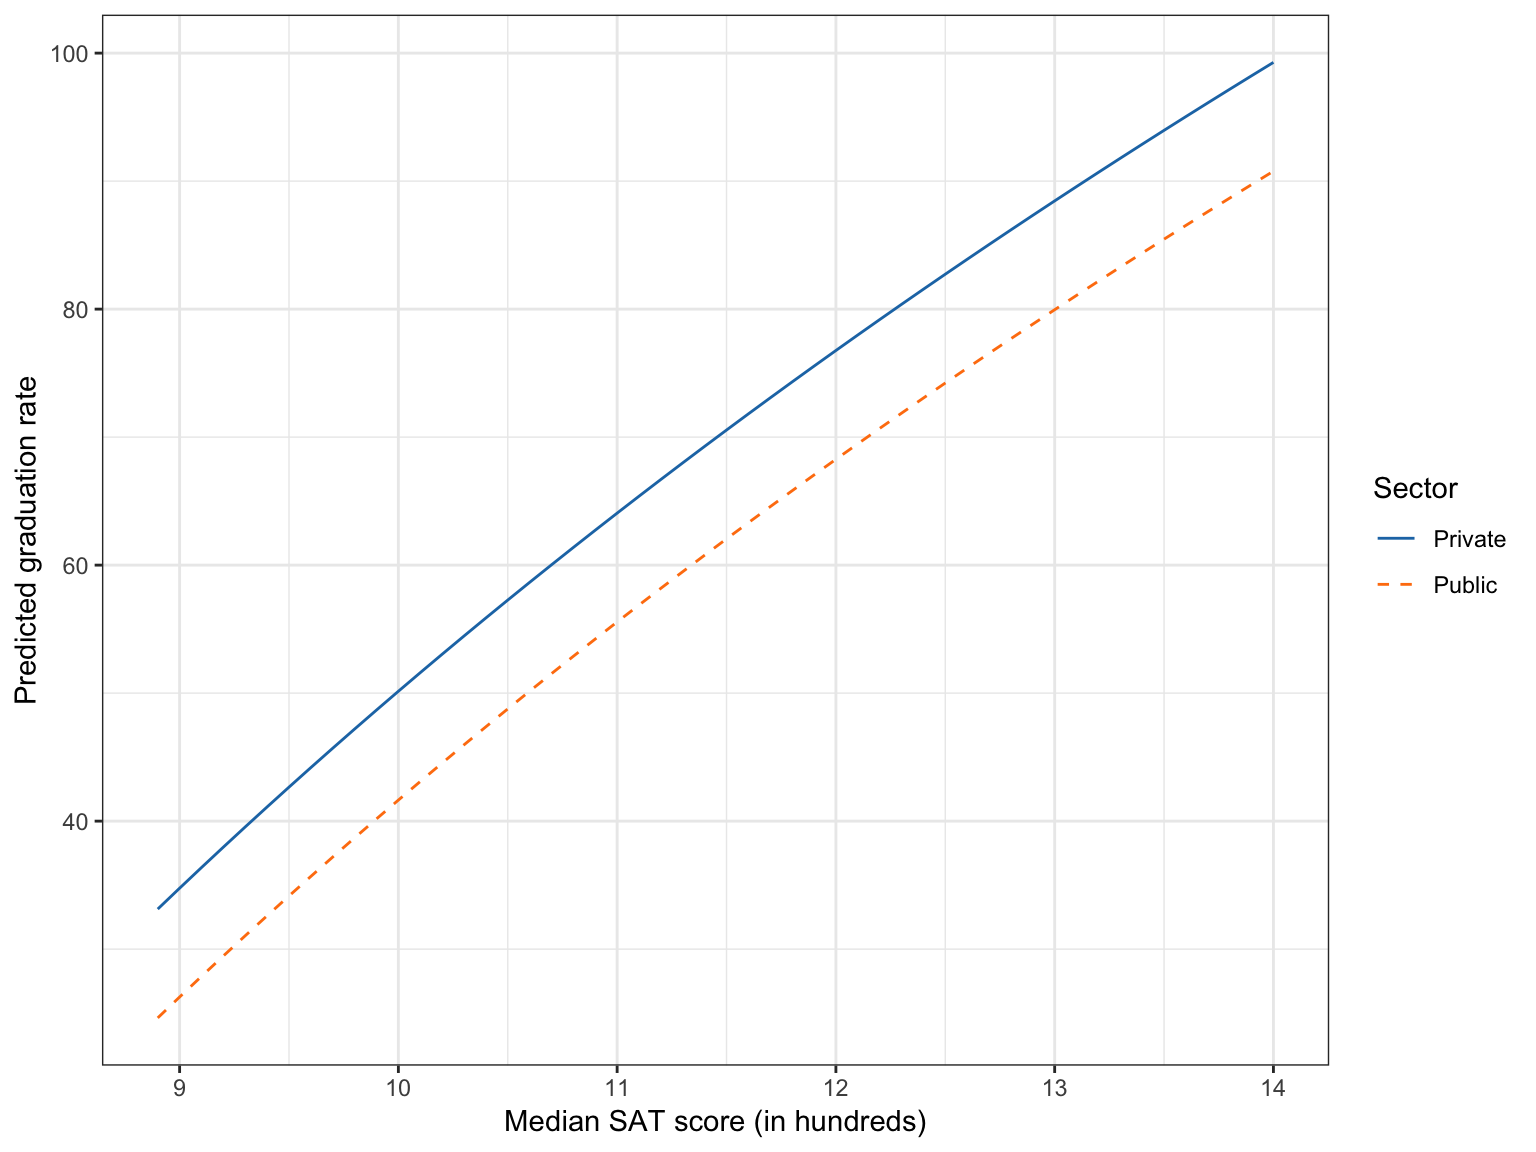
\includegraphics[width=0.5\linewidth]{epsy-8252-notes_files/figure-latex/unnamed-chunk-56-1} 

}

\caption{Predicted graduation rate as a function of median SAT score (in hundreds) and sector. The effect of SAT is log-linear.}\label{fig:unnamed-chunk-56}
\end{figure}

The plot shows the nonlinear, diminishing positive effect of SAT on graduation rate for both public and private schools. For schools with lower median SAT scores, there is a larger effect on graduation rates than for schools with higher median SAT scores (for both private and public schools). The plot also shows the controlled effect of sector. For schools with the same median SAT score, private schools have a higher predicted graduation rate than public schools, on average.

\hypertarget{polynomial-effects-vs.-log-transformations}{%
\section{Polynomial Effects vs.~Log-Transformations}\label{polynomial-effects-vs.-log-transformations}}

The inclusion of polynomial effects and the use of a log-transformation was to model the nonlinearity observed in the relationship between SAT scores and graduation rates. Both methods were successful in this endeavor. While either method could be used in practice to model nonlinearity, there are some considerations when making the choice of which may be more appropriate for a given modeling situation.

The first consideration is one of theory. The plot below shows the mathematical function for a log-transformed \(X\)-value (solid, black line) and for a quadratic polynomial of \(X\) (dashed, red line).

\begin{figure}

{\centering 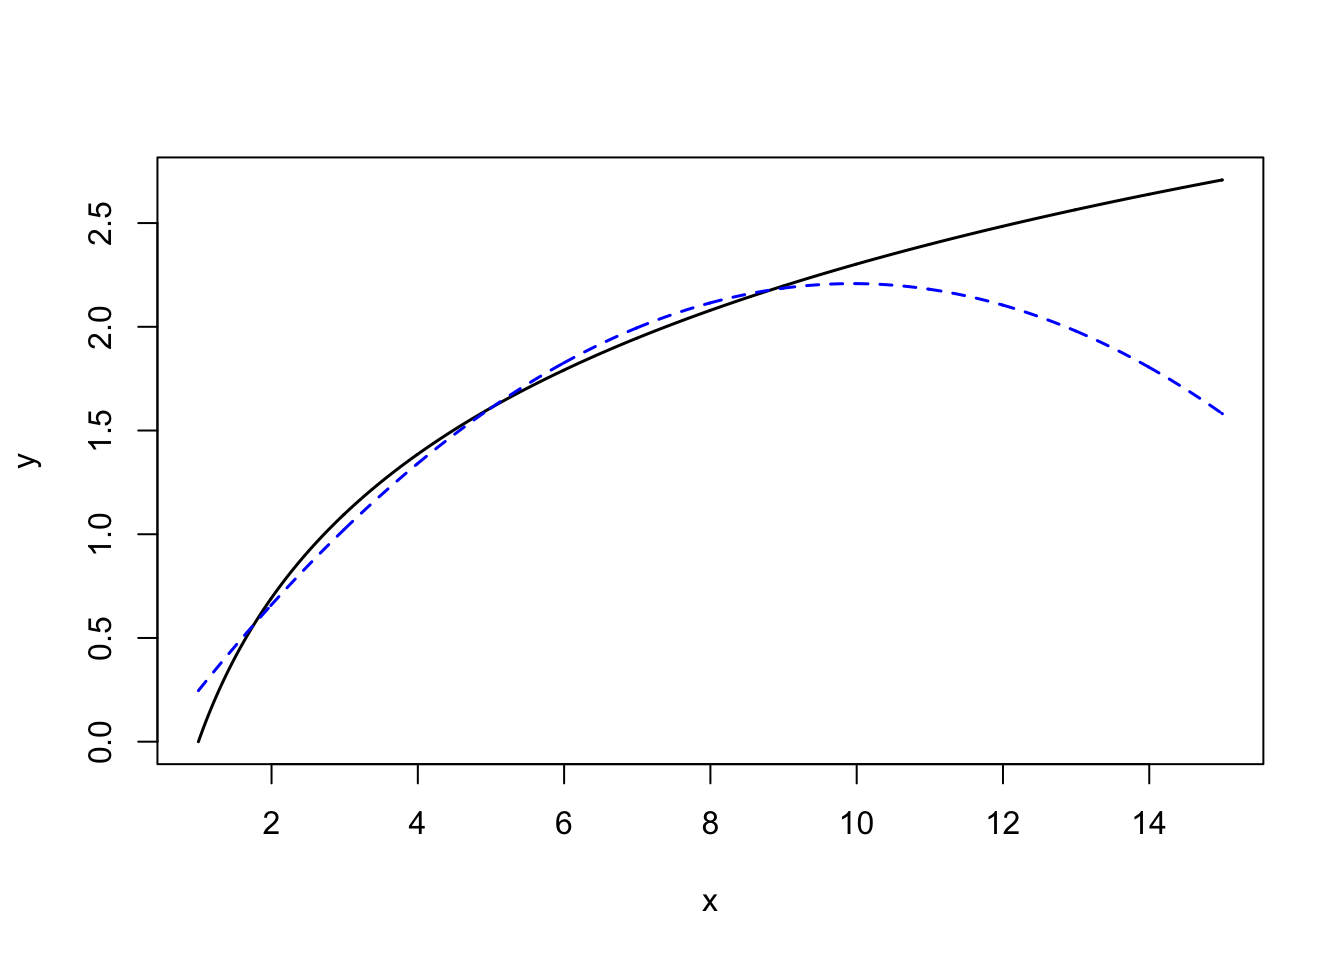
\includegraphics[width=3in]{epsy-8252-notes_files/figure-latex/unnamed-chunk-57-1} 

}

\caption{Comparison of quadratic (blue, dashed) and logarithmic (black, solid) functions of X.}\label{fig:unnamed-chunk-57}
\end{figure}

Both functions are nonlinear, however the polynomial function changes direction. For low values of \(X\), the function has a large positive effect. This effect diminishes as \(X\) gets bigger, and around \(X=9\) the effect is zero. For larger values of \(X\), the effect is actually negative. For the logarithmic function, the effect is always positive, but it diminishes as \(X\) gets larger. (Functions that constantly increase, or constantly decrease, are referred to as \emph{monotonic functions}.) Theoretically, these are very different ideas, and if substantive literature suggests one or the other, you should probably acknowledge that in the underlying statistical model that is fitted.

Empirically, the two functions are very similar especially within certain ranges of \(X\). For example, although the predictions from these models would be quite different for really high values of \(X\), if we only had data from the range of 2 to 8 (\(2\leq X \leq 8\)) both functions would produce similar residuals. In this case, the residuals would likely not suggest better fit for either of the two models. In this case, it might be prudent to think about Occam's Razor---if two competing models produce similar predictions, adopt the simpler model. Between these two functions, the \textbf{log-transformed model is simpler}; it has one predictor compared to the two predictors in the quadratic model. The mathematical models make this clear:

\[
\begin{split}
\mathbf{Polynomial:~}Y_i &= \beta_0 + \beta_1(X_i) + \beta_2(X_i^2) +\epsilon_i \\
\mathbf{Log\mbox{-}Transform:~}Y_i &= \beta_0 + \beta_1\bigg[\ln(X_i)\bigg] + \epsilon_i
\end{split}
\]

The quadratic polynomial model has two effects: a linear effect of \(X\) and a quadratic effect of \(X\) (remember it is an interaction model), while the model using the log-transformed predictor only has a single effect. If there is no theory to guide your model's functional form, and the residuals from the polynomial and log-transformed models seem to fit equally well, then the log-transformed model saves you a degree of freedom, and probably should be adopted.

\begin{center}\rule{0.5\linewidth}{\linethickness}\end{center}

\hypertarget{other-resources-1}{%
\section*{Other Resources}\label{other-resources-1}}
\addcontentsline{toc}{section}{Other Resources}

In addition to the notes and what we cover in class, there are many other resources for learning about log-transformations. Here are some resources that may be helpful in that endeavor:

\begin{itemize}
\tightlist
\item
  \href{https://www.cscu.cornell.edu/news/statnews/stnews83.pdf}{Interpreting Coefficients in Regression with Log-Transformed Variables}
\item
  \href{http://www.cazaar.com/ta/econ113/interpreting-beta}{Interpret Regression Coefficient Estimates}
\end{itemize}

\hypertarget{nonlinearity-log-transforming-the-outcome}{%
\chapter{Nonlinearity: Log-Transforming the Outcome}\label{nonlinearity-log-transforming-the-outcome}}

In this set of notes, you will learn about log-transforming the outcome variable in a regression model to account for nonlinearity and heterogeneity of variance.

\begin{center}\rule{0.5\linewidth}{\linethickness}\end{center}

\hypertarget{preparation-2}{%
\subsection*{Preparation}\label{preparation-2}}
\addcontentsline{toc}{subsection}{Preparation}

Before class you will need to read the following:

\begin{itemize}
\tightlist
\item
  Osborne, Jason (2002). \href{https://pareonline.net/getvn.asp?v=8\&n=6}{Notes on the use of data transformations}. \emph{Practical Assessment, Research \& Evaluation, 8}(6).
\end{itemize}

\begin{center}\rule{0.5\linewidth}{\linethickness}\end{center}

\hypertarget{dataset-and-research-question-1}{%
\section{Dataset and Research Question}\label{dataset-and-research-question-1}}

The data we will use in this set of notes, \emph{movies.csv} (see the \protect\hyperlink{movies}{data codebook} here), includes attributes for \(n=1,806\) movies.

\begin{Shaded}
\begin{Highlighting}[]
\CommentTok{# Load libraries}
\KeywordTok{library}\NormalTok{(broom)}
\KeywordTok{library}\NormalTok{(dplyr)}
\KeywordTok{library}\NormalTok{(ggplot2)}
\KeywordTok{library}\NormalTok{(readr)}
\KeywordTok{library}\NormalTok{(sm)}
\KeywordTok{library}\NormalTok{(tidyr)}

\CommentTok{# Import data}
\NormalTok{movies =}\StringTok{ }\KeywordTok{read_csv}\NormalTok{(}\DataTypeTok{file =} \StringTok{"~/Documents/github/epsy-8252/data/movies.csv"}\NormalTok{)}
\KeywordTok{head}\NormalTok{(movies)}
\end{Highlighting}
\end{Shaded}

\begin{verbatim}
# A tibble: 6 x 4
  title                      budget   age mpaa 
  <chr>                       <dbl> <dbl> <chr>
1 'Til There Was You           23      21 PG-13
2 10 Things I Hate About You   16      19 PG-13
3 100 Mile Rule                 1.1    16 R    
4 13 Going On 30               37      14 PG-13
5 13th Warrior, The            85      19 R    
6 15 Minutes                   42      17 R    
\end{verbatim}

Using these data, we will examine the relationship between age of a movie and budget.

\hypertarget{examine-relationship-between-age-and-budget}{%
\section{Examine Relationship between Age and Budget}\label{examine-relationship-between-age-and-budget}}

To being the analysis, we will examine the scatterplot between age and budget of our sample data.

\begin{Shaded}
\begin{Highlighting}[]
\KeywordTok{ggplot}\NormalTok{(}\DataTypeTok{data =}\NormalTok{ movies, }\KeywordTok{aes}\NormalTok{(}\DataTypeTok{x =}\NormalTok{ age, }\DataTypeTok{y =}\NormalTok{ budget)) }\OperatorTok{+}
\StringTok{  }\KeywordTok{geom_point}\NormalTok{() }\OperatorTok{+}
\StringTok{  }\KeywordTok{geom_smooth}\NormalTok{(}\DataTypeTok{se =} \OtherTok{FALSE}\NormalTok{) }\OperatorTok{+}
\StringTok{  }\KeywordTok{theme_bw}\NormalTok{() }\OperatorTok{+}
\StringTok{  }\KeywordTok{xlab}\NormalTok{(}\StringTok{"Movie age"}\NormalTok{) }\OperatorTok{+}
\StringTok{  }\KeywordTok{ylab}\NormalTok{(}\StringTok{"Movie Budget (in millions of dollars)"}\NormalTok{)}
\end{Highlighting}
\end{Shaded}

\begin{figure}

{\centering 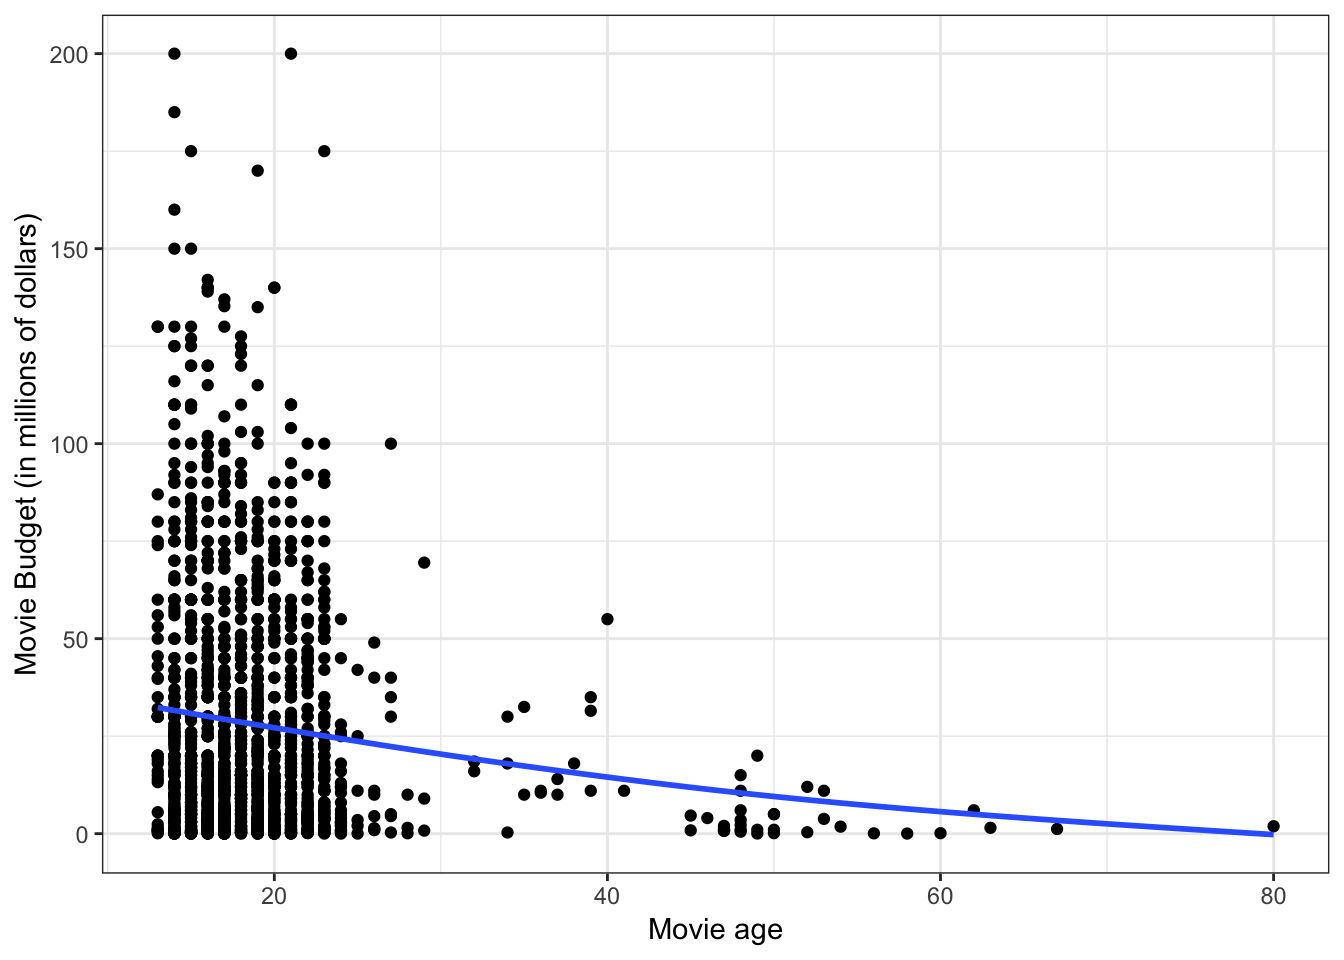
\includegraphics[width=0.5\linewidth]{epsy-8252-notes_files/figure-latex/unnamed-chunk-61-1} 

}

\caption{Scatterplot between age and budget. The loess smoother is also displayed.}\label{fig:unnamed-chunk-61}
\end{figure}

The scatterplot suggests two potential problems with fitting a linear model to the data:

\begin{itemize}
\tightlist
\item
  The relationship is slightly curvilinear.
\item
  The variation in budget for more recent movies is much greater than the variation in budget for older movies (heteroskedasticity).
\end{itemize}

We can see this much more clearly in the scatterplot of residuals versus fitted values from a fitted linear model.

\begin{Shaded}
\begin{Highlighting}[]
\CommentTok{# Fit model}
\NormalTok{lm}\FloatTok{.1}\NormalTok{ =}\StringTok{ }\KeywordTok{lm}\NormalTok{(budget }\OperatorTok{~}\StringTok{ }\DecValTok{1} \OperatorTok{+}\StringTok{ }\NormalTok{age, }\DataTypeTok{data =}\NormalTok{ movies)}

\CommentTok{# Obtain residuals and fitted values}
\NormalTok{out_}\DecValTok{1}\NormalTok{ =}\StringTok{ }\KeywordTok{augment}\NormalTok{(lm}\FloatTok{.1}\NormalTok{)}

\CommentTok{# Density plot of the residuals}
\KeywordTok{sm.density}\NormalTok{(out_}\DecValTok{1}\OperatorTok{$}\NormalTok{.std.resid, }\DataTypeTok{model =} \StringTok{"normal"}\NormalTok{, }\DataTypeTok{xlab =} \StringTok{"Standardized residuals"}\NormalTok{)}

\CommentTok{# Residuals versus fitted values}
\KeywordTok{ggplot}\NormalTok{(}\DataTypeTok{data =}\NormalTok{ out_}\DecValTok{1}\NormalTok{, }\KeywordTok{aes}\NormalTok{(}\DataTypeTok{x =}\NormalTok{ .fitted, }\DataTypeTok{y =}\NormalTok{ .std.resid)) }\OperatorTok{+}
\StringTok{  }\KeywordTok{geom_point}\NormalTok{() }\OperatorTok{+}
\StringTok{  }\KeywordTok{geom_hline}\NormalTok{(}\DataTypeTok{yintercept =} \DecValTok{0}\NormalTok{) }\OperatorTok{+}
\StringTok{  }\KeywordTok{geom_smooth}\NormalTok{() }\OperatorTok{+}
\StringTok{  }\KeywordTok{theme_bw}\NormalTok{() }\OperatorTok{+}
\StringTok{  }\KeywordTok{xlab}\NormalTok{(}\StringTok{"Fitted values"}\NormalTok{) }\OperatorTok{+}
\StringTok{  }\KeywordTok{ylab}\NormalTok{(}\StringTok{"Standardized residuals"}\NormalTok{)}
\end{Highlighting}
\end{Shaded}

\begin{figure}

{\centering 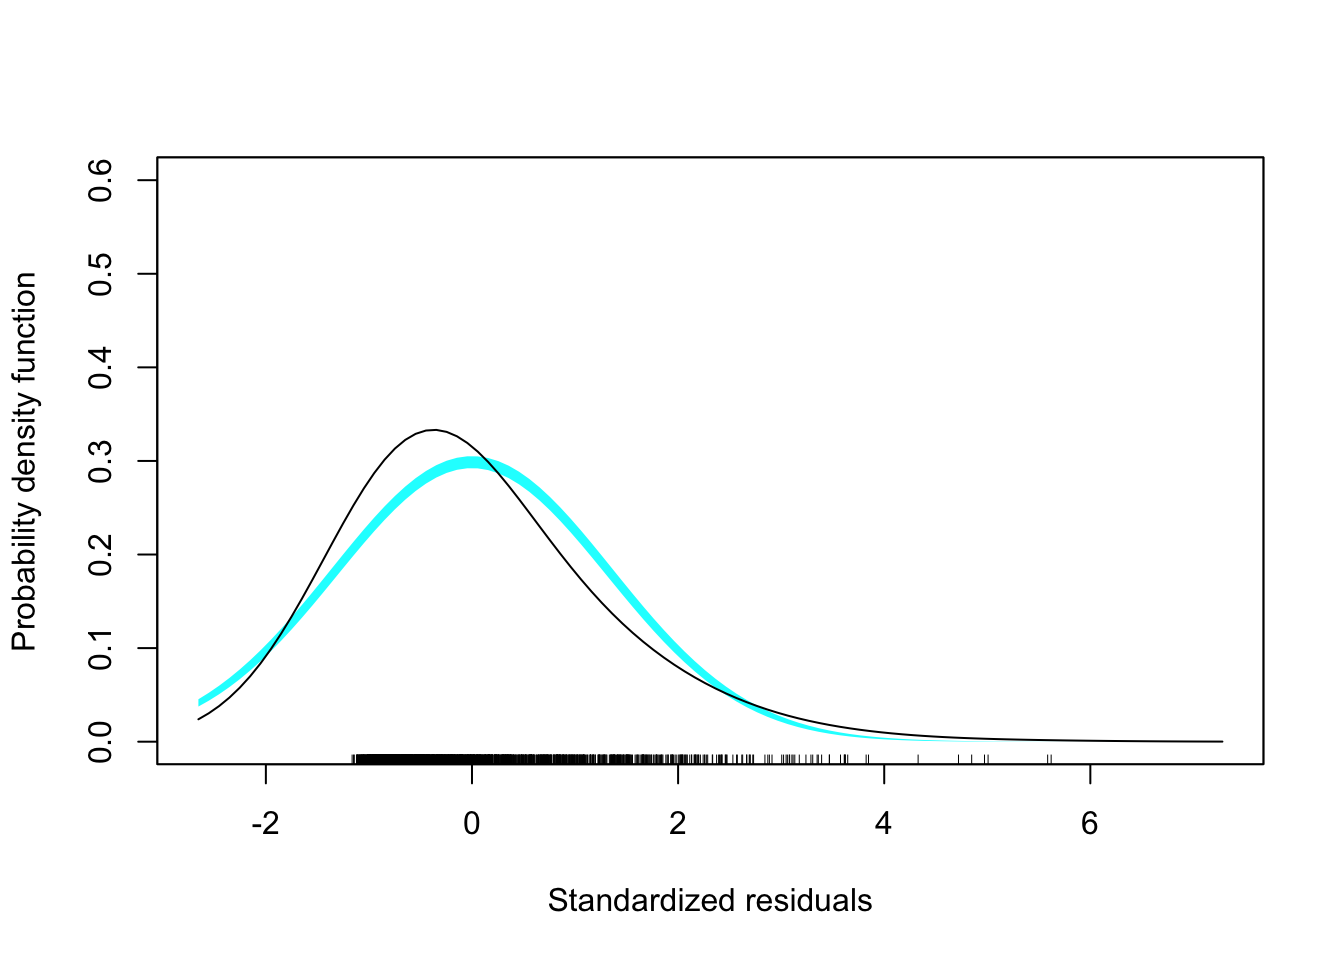
\includegraphics[width=0.4\linewidth]{epsy-8252-notes_files/figure-latex/unnamed-chunk-62-1} 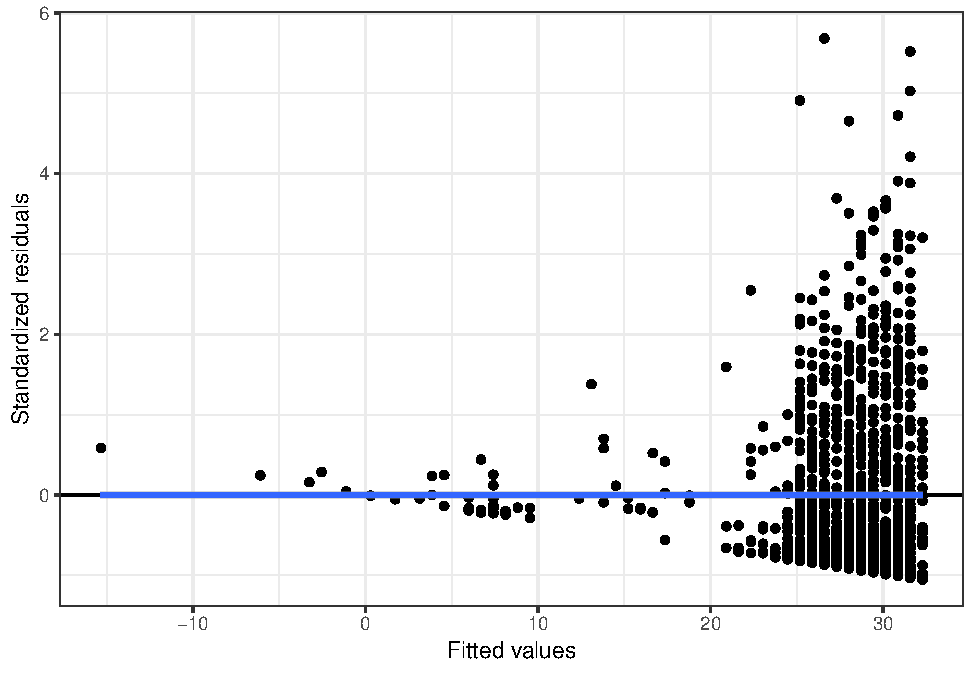
\includegraphics[width=0.4\linewidth]{epsy-8252-notes_files/figure-latex/unnamed-chunk-62-2} 

}

\caption{Residual plots from regressing budget on age.}\label{fig:unnamed-chunk-62}
\end{figure}

These plots suggest violations of the normality assumption (the marginal distribution of the residuals is right-skewed) and of the assumption of homoskedasticity. Because of the large sample size, violation the linearity assumption is more difficult to see in this plot.

\hypertarget{transform-the-outcome-using-the-natural-logarithm-base-e}{%
\section{Transform the Outcome Using the Natural Logarithm (Base-e)}\label{transform-the-outcome-using-the-natural-logarithm-base-e}}

To alleviate problems of non-normality when the conditional distributions are right-skewed (or have high-end outliers) OR to alleviate heteroskedasticity, we can mathematically transform the outcome using a logarithm. Any base can be used for the logarithm, but we will transform the outcome using the natural logarithm because of the interpretive value.

First, we will create the log-transformed variable as a new column in the data, and then we will use the log-transformed budget (rather than raw budget) in any analyses.

\begin{Shaded}
\begin{Highlighting}[]
\CommentTok{# Create log-transformed budget}
\NormalTok{movies =}\StringTok{ }\NormalTok{movies }\OperatorTok\StringTok{ }
\StringTok{  }\KeywordTok{mutate}\NormalTok{(}
    \DataTypeTok{Lbudget =} \KeywordTok{log}\NormalTok{(budget)}
\NormalTok{    )}

\CommentTok{# Examine data}
\KeywordTok{head}\NormalTok{(movies)}
\end{Highlighting}
\end{Shaded}

\begin{verbatim}
# A tibble: 6 x 5
  title                      budget   age mpaa  Lbudget
  <chr>                       <dbl> <dbl> <chr>   <dbl>
1 'Til There Was You           23      21 PG-13  3.14  
2 10 Things I Hate About You   16      19 PG-13  2.77  
3 100 Mile Rule                 1.1    16 R      0.0953
4 13 Going On 30               37      14 PG-13  3.61  
5 13th Warrior, The            85      19 R      4.44  
6 15 Minutes                   42      17 R      3.74  
\end{verbatim}

Recall that the logarithm is the inverse function of an exponent. As an example, consider the budget and log-transformed budget for \emph{'Til There Was You}.

\[
\begin{split}
\ln(\textrm{Budget}) &= 3.135 \\
\ln(23.0) &= 3.135 \\
\end{split}
\]

Or,

\[
e^{3.135} = 23.0
\]

Remember, the logarithm answers the mathematical question:

\begin{quote}
\(e\) to what power is equal to 23.0?
\end{quote}

\hypertarget{re-analyze-using-the-log-transformed-budget}{%
\section{Re-analyze using the Log-Transformed Budget}\label{re-analyze-using-the-log-transformed-budget}}

Now we will re-examine the scatterplot using the log-transformed outcome to see how this transformation affects the relationship.

\begin{Shaded}
\begin{Highlighting}[]
\CommentTok{# Scatterplot}
\KeywordTok{ggplot}\NormalTok{(}\DataTypeTok{data =}\NormalTok{ movies, }\KeywordTok{aes}\NormalTok{(}\DataTypeTok{x =}\NormalTok{ age, }\DataTypeTok{y =}\NormalTok{ Lbudget)) }\OperatorTok{+}
\StringTok{  }\KeywordTok{geom_point}\NormalTok{() }\OperatorTok{+}
\StringTok{  }\KeywordTok{geom_smooth}\NormalTok{(}\DataTypeTok{se =} \OtherTok{FALSE}\NormalTok{) }\OperatorTok{+}
\StringTok{  }\KeywordTok{theme_bw}\NormalTok{() }\OperatorTok{+}
\StringTok{  }\KeywordTok{xlab}\NormalTok{(}\StringTok{"Movie age"}\NormalTok{) }\OperatorTok{+}
\StringTok{  }\KeywordTok{ylab}\NormalTok{(}\StringTok{"ln(Movie Budget)"}\NormalTok{)}
\end{Highlighting}
\end{Shaded}

\begin{figure}

{\centering 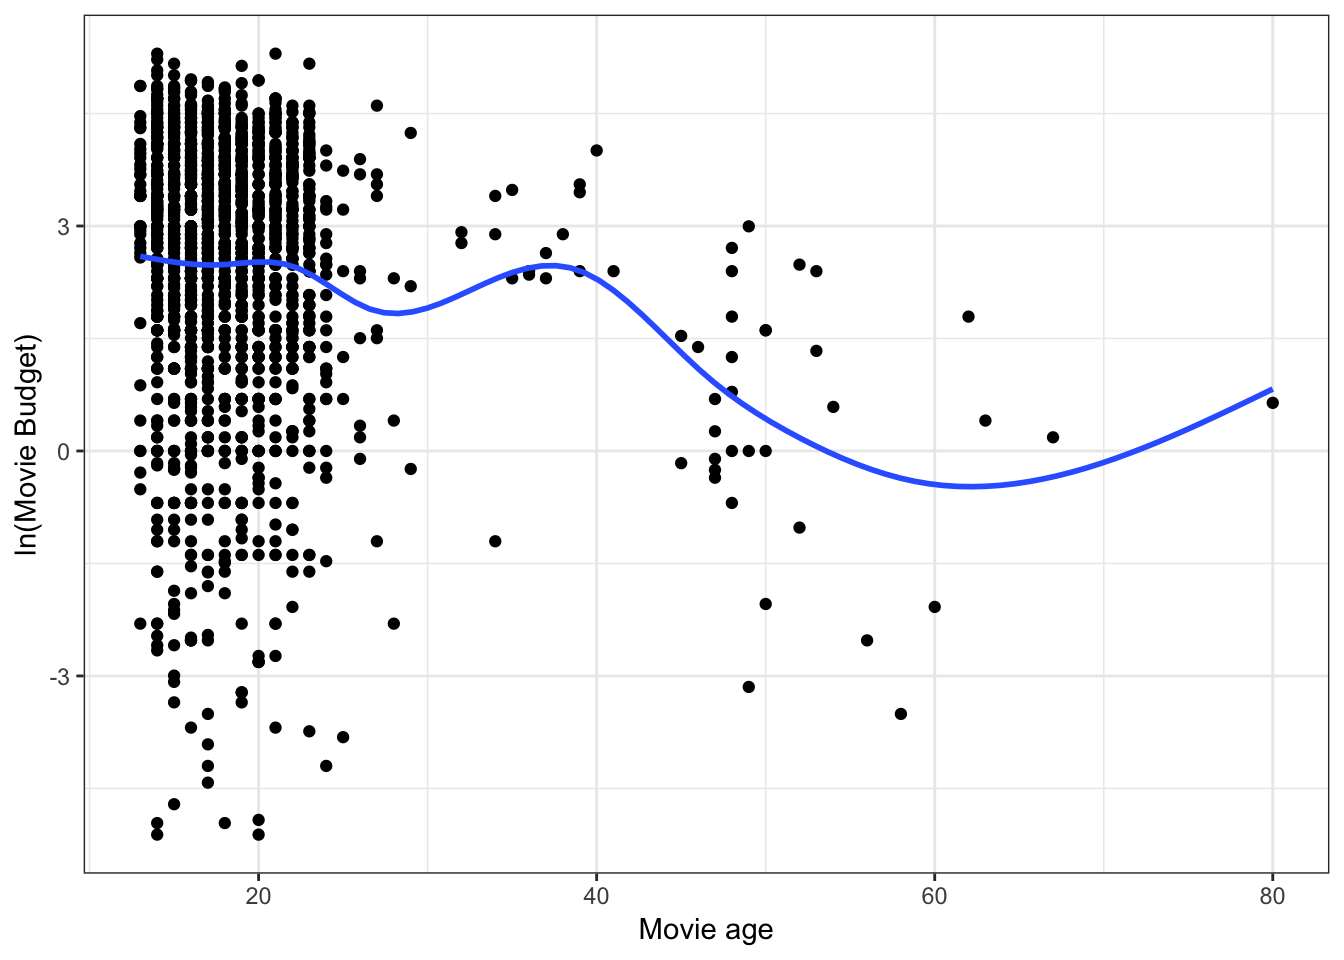
\includegraphics[width=0.5\linewidth]{epsy-8252-notes_files/figure-latex/unnamed-chunk-64-1} 

}

\caption{Scatterplot between age and log-transformed budget. The loess smoother is also displayed.}\label{fig:unnamed-chunk-64}
\end{figure}

Log-transforming the outcome has drastically affected the scale for the outcome. Has this helped us better meet the assumptions? Again, we should examine the residual plots.

\begin{Shaded}
\begin{Highlighting}[]
\CommentTok{# Fit model}
\NormalTok{lm}\FloatTok{.2}\NormalTok{ =}\StringTok{ }\KeywordTok{lm}\NormalTok{(Lbudget }\OperatorTok{~}\StringTok{ }\DecValTok{1} \OperatorTok{+}\StringTok{ }\NormalTok{age, }\DataTypeTok{data =}\NormalTok{ movies)}

\CommentTok{# Obtain residuals and fitted values}
\NormalTok{out_}\DecValTok{2}\NormalTok{ =}\StringTok{ }\KeywordTok{augment}\NormalTok{(lm}\FloatTok{.2}\NormalTok{)}

\CommentTok{# Density plot of the residuals}
\KeywordTok{sm.density}\NormalTok{(out_}\DecValTok{2}\OperatorTok{$}\NormalTok{.std.resid, }\DataTypeTok{model =} \StringTok{"normal"}\NormalTok{, }\DataTypeTok{xlab =} \StringTok{"Standardized residuals"}\NormalTok{)}

\CommentTok{# Residuals versus fitted values}
\KeywordTok{ggplot}\NormalTok{(}\DataTypeTok{data =}\NormalTok{ out_}\DecValTok{2}\NormalTok{, }\KeywordTok{aes}\NormalTok{(}\DataTypeTok{x =}\NormalTok{ .fitted, }\DataTypeTok{y =}\NormalTok{ .std.resid)) }\OperatorTok{+}
\StringTok{  }\KeywordTok{geom_point}\NormalTok{() }\OperatorTok{+}
\StringTok{  }\KeywordTok{geom_hline}\NormalTok{(}\DataTypeTok{yintercept =} \DecValTok{0}\NormalTok{) }\OperatorTok{+}
\StringTok{  }\KeywordTok{geom_smooth}\NormalTok{() }\OperatorTok{+}
\StringTok{  }\KeywordTok{theme_bw}\NormalTok{() }\OperatorTok{+}
\StringTok{  }\KeywordTok{xlab}\NormalTok{(}\StringTok{"Fitted values"}\NormalTok{) }\OperatorTok{+}
\StringTok{  }\KeywordTok{ylab}\NormalTok{(}\StringTok{"Standardized residuals"}\NormalTok{)}
\end{Highlighting}
\end{Shaded}

\begin{figure}

{\centering 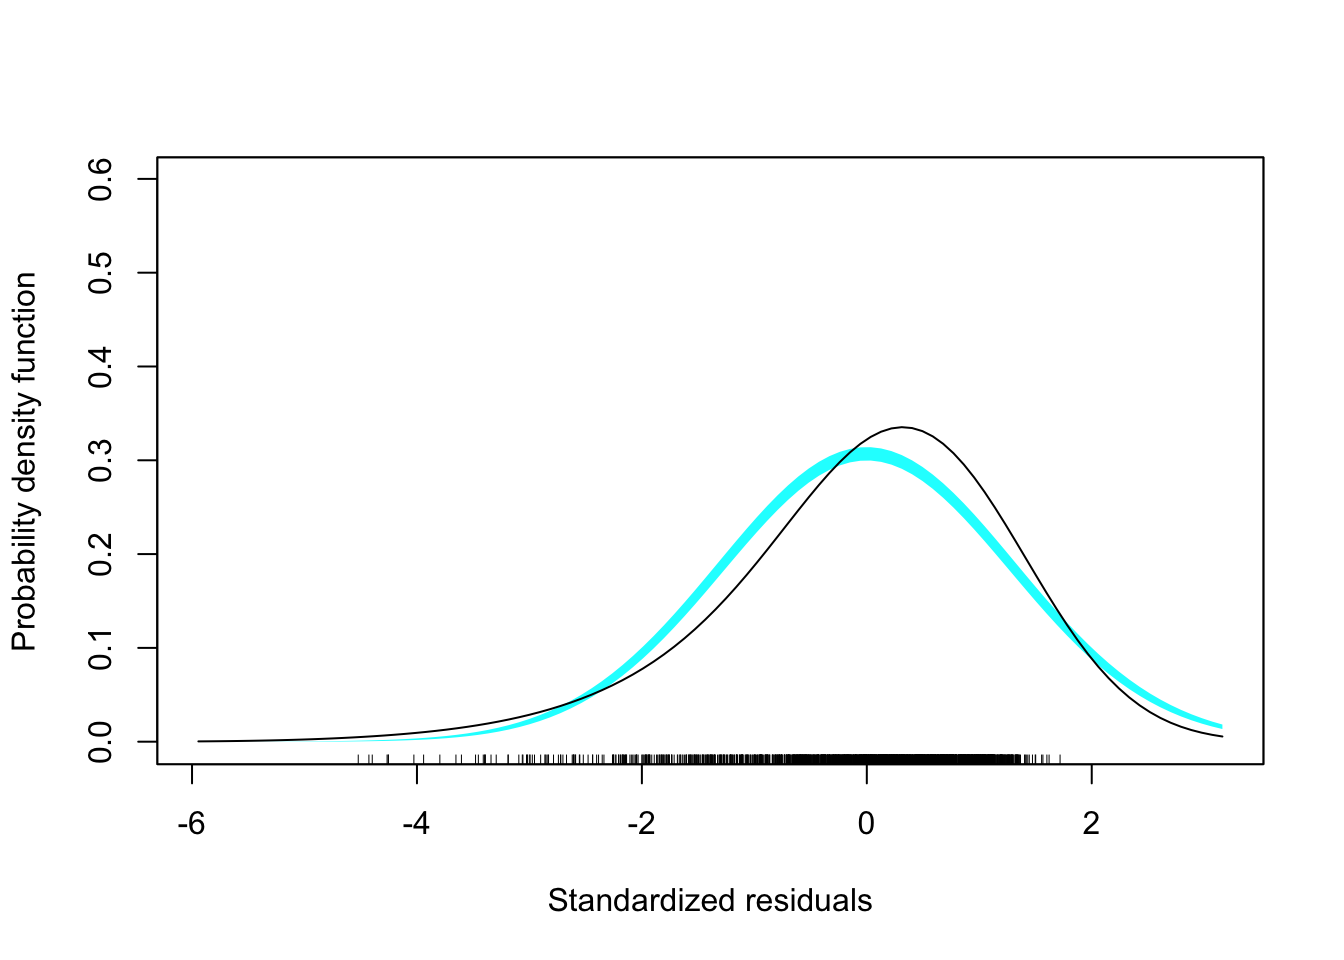
\includegraphics[width=0.4\linewidth]{epsy-8252-notes_files/figure-latex/unnamed-chunk-65-1} 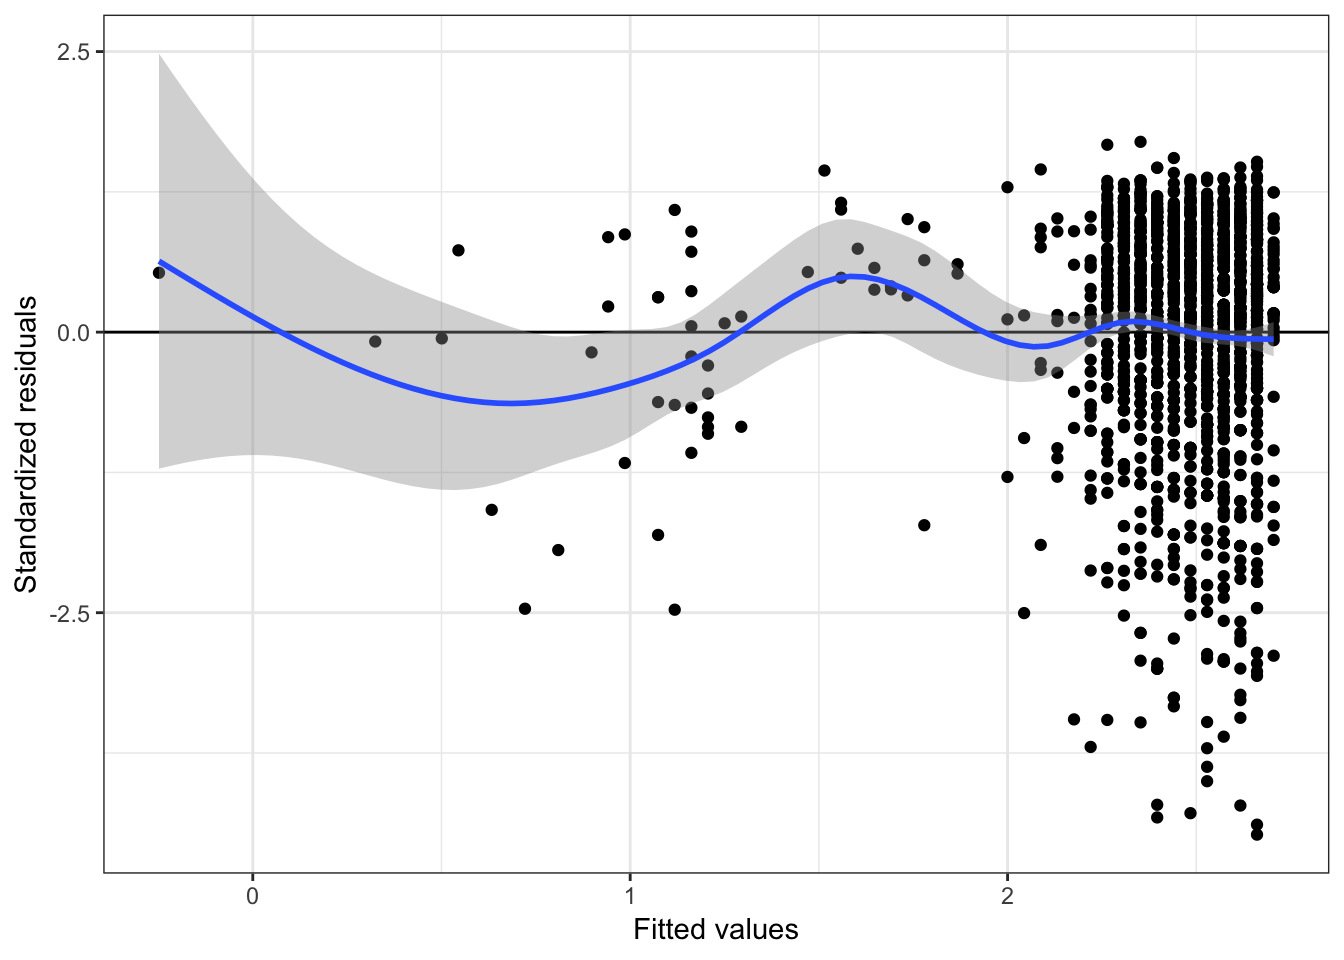
\includegraphics[width=0.4\linewidth]{epsy-8252-notes_files/figure-latex/unnamed-chunk-65-2} 

}

\caption{Residual plots from regressing the natural logarithm of budget on age.}\label{fig:unnamed-chunk-65}
\end{figure}

These plots still suggest violations of the normality assumption (the marginal distribution of the residuals is now left-skewed). The assumption of homoskedasticity also seems still violated, although much less. Most importantly, however, is the assumption of linearity now seems satisfied.

\hypertarget{interpreting-the-regression-output}{%
\section{Interpreting the Regression Output}\label{interpreting-the-regression-output}}

Let's examine the output from the model in which we regressed the log-transformed budget on age.

\begin{Shaded}
\begin{Highlighting}[]
\CommentTok{# Model-level output}
\KeywordTok{glance}\NormalTok{(lm}\FloatTok{.2}\NormalTok{)}
\end{Highlighting}
\end{Shaded}

\begin{verbatim}
# A tibble: 1 x 11
  r.squared adj.r.squared sigma statistic  p.value    df logLik   AIC   BIC
      <dbl>         <dbl> <dbl>     <dbl>    <dbl> <int>  <dbl> <dbl> <dbl>
1    0.0213        0.0208  1.74      39.3 4.60e-10     2 -3560. 7125. 7142.
# ... with 2 more variables: deviance <dbl>, df.residual <int>
\end{verbatim}

The model-level summary information suggests that differences in movies' ages explains 2.1\% of the variation in budget. (Remember, explaining variation in log-budget is the same as explaining variation in budget). Although this is a small amount of variation, it is statistically significant, \(F(1,1804)=39.27\), \(p<0.001\).

\begin{Shaded}
\begin{Highlighting}[]
\CommentTok{# Coefficient-level output}
\KeywordTok{tidy}\NormalTok{(lm}\FloatTok{.2}\NormalTok{)}
\end{Highlighting}
\end{Shaded}

\begin{verbatim}
# A tibble: 2 x 5
  term        estimate std.error statistic   p.value
  <chr>          <dbl>     <dbl>     <dbl>     <dbl>
1 (Intercept)   3.28     0.139       23.6  1.69e-107
2 age          -0.0441   0.00703     -6.27 4.60e- 10
\end{verbatim}

From the coefficient-level output the fitted equation is:

\[
\ln\left(\hat{\mathrm{Budget}_i}\right) = 3.28 - 0.04(\mathrm{Age}_i)
\]

With log-transformations, there are two possible interpretations we can offer. The first is to interpret the coefficients using the log-transformed values. These we interpret in the exact same way we do any other regression coefficients (except we use log-outcome instead of outcome):

\begin{itemize}
\tightlist
\item
  The intercept, \(\hat{\beta_0} = 3.28\), is the average predicted log-budget for movies made in 2019 (Age = 0).
\item
  The slope, \(\hat{\beta_1} = -0.04\), indicates that each one-year difference in age is associated with a log-budget that differ by \(-0.04\), on average.
\end{itemize}

\hypertarget{back-transforming-a-more-useful-interpretation}{%
\subsection{Back-Transforming: A More Useful Interpretation}\label{back-transforming-a-more-useful-interpretation}}

A second, probably more useful, interpretation is to back-transform log-budget to budget. To think about how to do this, we first consider a more general expression of the fitted linear model:

\[
\ln\left(\hat{Y}_i\right) = \hat\beta_0 + \hat\beta_1(X_{i})
\]

The left-hand side of the equation is in the log-transformed metric, which drives our interpretations. If we want to instead, interpret using the raw metric of \(Y\), we need to back-transform from \(\ln(Y)\) to \(Y\). To back-transform, we use the inverse function, which is to exponentiate using the base of the logarithm, in our case, base-\(e\).

\[
e^{\ln(Y_i)} = Y_i
\]

If we exponentiate the left-hand side of the equation, to maintain the equality, we also need to exponentiate the right-hand side of the equation.

\[
e^{\ln(Y_i)} = e^{\hat\beta_0 + \hat\beta_1(X_{i})}
\]

Then we use rules of exponents to simplify this.

\[
Y_i = e^{\hat\beta_0} \times e^{\hat\beta_1(X_{i})}
\]

For our example, when we exponentiate both sides of the fitted equation:

\[
\hat{\mathrm{Budget}_i} = e^{3.28} \times e^{-0.04(\mathrm{Age}_i)}
\]

\hypertarget{substituting-in-values-for-age-to-interpret-effects}{%
\subsection{Substituting in Values for Age to Interpret Effects}\label{substituting-in-values-for-age-to-interpret-effects}}

To interpret the effects (which are now interpreted using budget---not log-budget) we can substitute in the different values for age and solve. For example when Age = 0:

\[
\begin{split}
\hat{\mathrm{Budget}_i} &= e^{3.28} \times e^{-0.04(0)}\\
&= 26.58 \times 1 \\
&= 26.58
\end{split}
\]

The predicted budget for a movie made in 2019 is 26.58 million dollars. How about a movie that was made in 2018 (a one-year difference)?

\[
\begin{split}
\hat{\mathrm{Budget}_i} &= e^{3.28} \times e^{-0.04(1)}\\
&= 26.58 \times 0.96 \\
&= 25.54
\end{split}
\]

The predicted budget for a movie made in 2019 is 25.54 million dollars. This is 0.96 TIMES the budget of a movie made in 2018.

Rather than using the language of \textbf{TIMES difference} you could also use the language of \textbf{fold difference}. In this case the slope coefficient would be interpreted as,

\begin{quote}
Each one-year difference in age is associated with a 0.95-fold difference in budget, on average.
\end{quote}

Simply put, when we back-transform from interpretations of log-\(Y\) to \(Y\) the interpretations are multiplicatively related to the intercept rather than additive. We can obtain these multiplicative values (and the back-transformed intercept) by using the \texttt{exp()} function to exponentiate the coefficients from the fitted model, which we obtain using the \texttt{coef()} function.

\begin{Shaded}
\begin{Highlighting}[]
\KeywordTok{exp}\NormalTok{(}\KeywordTok{coef}\NormalTok{(lm}\FloatTok{.2}\NormalTok{))}
\end{Highlighting}
\end{Shaded}

\begin{verbatim}
(Intercept)         age 
    26.5261      0.9569 
\end{verbatim}

\hypertarget{approximate-interpretation-of-the-slope}{%
\subsection{Approximate Interpretation of the Slope}\label{approximate-interpretation-of-the-slope}}

Remember that by using the natural logarithm we can interpret the effects as percent change. Rather than saying that a movie made in 2018 is predicted to have a budget that is 0.96 TIMES that of a movie made in 2019, we can directly interpret the slope as the percent change. Thus \(\hat{\beta_1}=-0.04\) can be interpreted as:

\begin{quote}
Each one-year difference in age is associated with a four percent decrease in budget, on average.
\end{quote}

If you want the specific mathematical change in budget, find \(1 - e^{\hat{\beta_1}}\).

\begin{Shaded}
\begin{Highlighting}[]
\DecValTok{1} \OperatorTok{-}\StringTok{ }\KeywordTok{exp}\NormalTok{(}\OperatorTok{-}\FloatTok{0.04}\NormalTok{)}
\end{Highlighting}
\end{Shaded}

\begin{verbatim}
[1] 0.03921
\end{verbatim}

If you use the language of percent decrease/increase, be very careful. \emph{Percent change} and \emph{percentage change} are sometimes interpreted differently! It is generally more clear to use the \emph{X-fold difference} language.

\hypertarget{plotting-the-fitted-model-1}{%
\section{Plotting the Fitted Model}\label{plotting-the-fitted-model-1}}

As always, we can plot the fitted model to aid in interpretation. To do this we will create a sequence of ages, predict the log-budget using the fitted model, and then back-transform the log-budgets to raw budget.

\begin{Shaded}
\begin{Highlighting}[]
\CommentTok{# Set up data}
\NormalTok{plot_data =}\StringTok{ }\KeywordTok{crossing}\NormalTok{(}
    \DataTypeTok{age =} \KeywordTok{seq}\NormalTok{(}\DataTypeTok{from =} \DecValTok{13}\NormalTok{, }\DataTypeTok{to =} \DecValTok{80}\NormalTok{, }\DataTypeTok{by =} \DecValTok{1}\NormalTok{)}
\NormalTok{    ) }\OperatorTok
\StringTok{  }\KeywordTok{mutate}\NormalTok{(}
    \CommentTok{# Predict}
    \DataTypeTok{yhat =} \KeywordTok{predict}\NormalTok{(lm}\FloatTok{.2}\NormalTok{, }\DataTypeTok{newdata =}\NormalTok{ .)}
\NormalTok{  )}

\CommentTok{# Examine data}
\KeywordTok{head}\NormalTok{(plot_data)}
\end{Highlighting}
\end{Shaded}

\begin{verbatim}
# A tibble: 6 x 2
    age  yhat
  <dbl> <dbl>
1    13  2.71
2    14  2.66
3    15  2.62
4    16  2.57
5    17  2.53
6    18  2.48
\end{verbatim}

\begin{Shaded}
\begin{Highlighting}[]
\CommentTok{# Back-transform the log-budgets}
\NormalTok{plot_data =}\StringTok{ }\NormalTok{plot_data }\OperatorTok
\StringTok{  }\KeywordTok{mutate}\NormalTok{(}
    \DataTypeTok{budget =} \KeywordTok{exp}\NormalTok{(yhat)}
\NormalTok{  )}

\CommentTok{# Examine data}
\KeywordTok{head}\NormalTok{(plot_data)}
\end{Highlighting}
\end{Shaded}

\begin{verbatim}
# A tibble: 6 x 3
    age  yhat budget
  <dbl> <dbl>  <dbl>
1    13  2.71   15.0
2    14  2.66   14.3
3    15  2.62   13.7
4    16  2.57   13.1
5    17  2.53   12.5
6    18  2.48   12.0
\end{verbatim}

\begin{Shaded}
\begin{Highlighting}[]
\CommentTok{# Plot}
\KeywordTok{ggplot}\NormalTok{(}\DataTypeTok{data =}\NormalTok{ plot_data, }\KeywordTok{aes}\NormalTok{(}\DataTypeTok{x =}\NormalTok{ age, }\DataTypeTok{y =}\NormalTok{ budget)) }\OperatorTok{+}
\StringTok{    }\KeywordTok{geom_line}\NormalTok{() }\OperatorTok{+}
\StringTok{    }\KeywordTok{theme_bw}\NormalTok{() }\OperatorTok{+}
\StringTok{  }\KeywordTok{xlab}\NormalTok{(}\StringTok{"Age"}\NormalTok{) }\OperatorTok{+}
\StringTok{  }\KeywordTok{ylab}\NormalTok{(}\StringTok{"Predicted budget (in millions of U.S. dollars)"}\NormalTok{)}
\end{Highlighting}
\end{Shaded}

\begin{figure}

{\centering 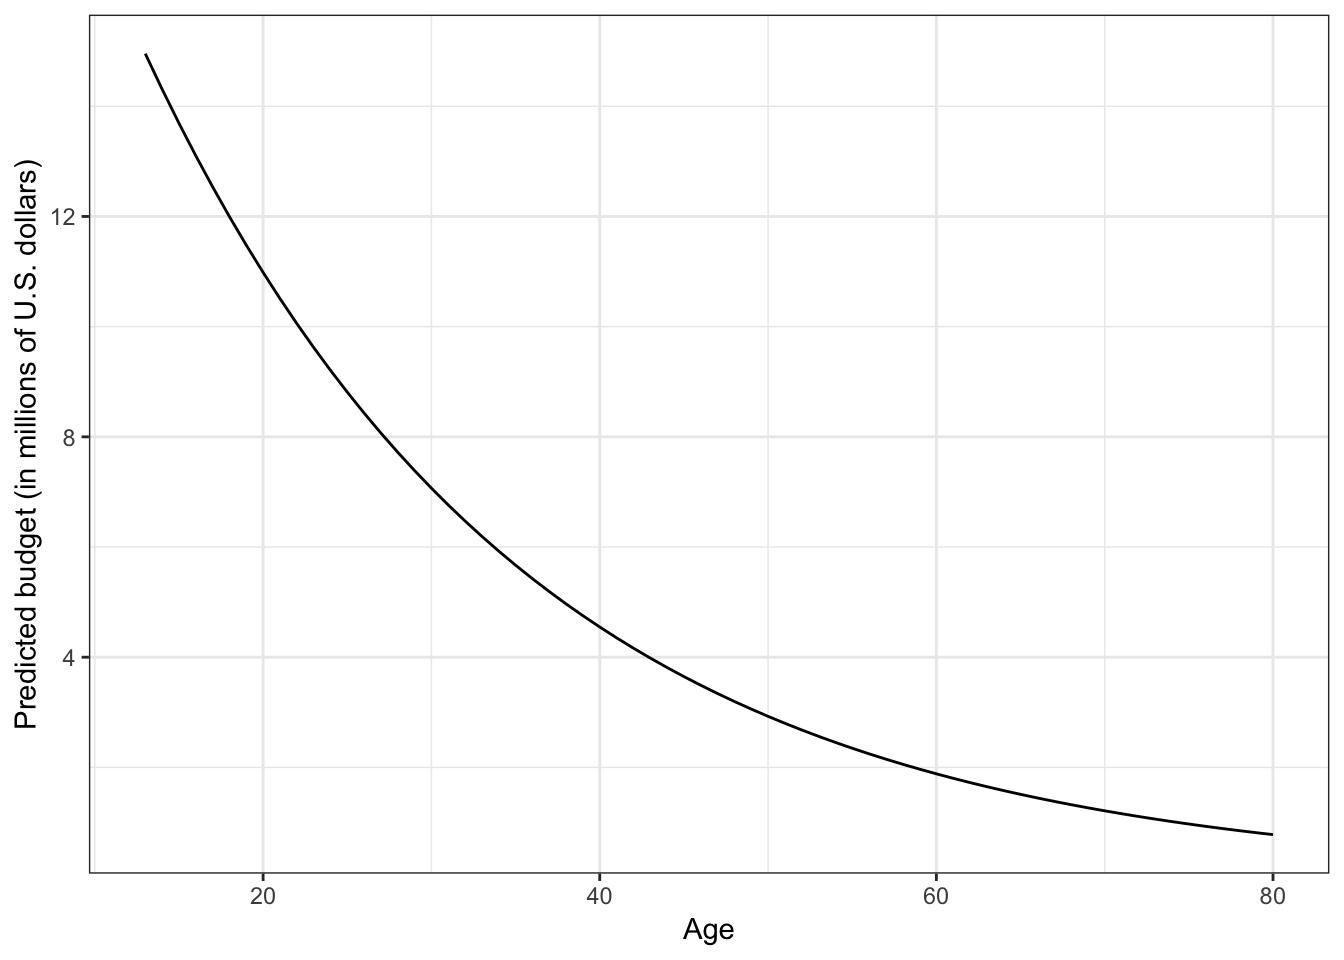
\includegraphics[width=0.5\linewidth]{epsy-8252-notes_files/figure-latex/unnamed-chunk-70-1} 

}

\caption{Plot of the predicted movie budget as a function of its age. The non-linearity in the plot indicates that there is a diminishing negative effect of age on budget.}\label{fig:unnamed-chunk-70}
\end{figure}

Based on this plot, we see the non-linear, negative effect of age on budget. In other words, older movies tend to have a smaller budget, on average, but this decrease is not constant. This pattern of non-linear decline is referred to as \emph{exponential decay}.

Although this function has a different look than the function we saw in the previous unit (it is negative rather than positive), it is also a \emph{monotonic} function (no change in direction).

\hypertarget{relationship-between-mpaa-rating-and-budget}{%
\section{Relationship between MPAA Rating and Budget}\label{relationship-between-mpaa-rating-and-budget}}

We also may want to control for differences in MPAA rating. Before we fit the multiple regression model, however, we will first explore whether MPAA rating is a useful covariate by seeing whether there are differences in budget between PG, PG-13m and R rated movies. Since we log-transformed budget (the outcome) in the previous analysis we will need to use the log-transformed outcome in this exploration as well.

\begin{Shaded}
\begin{Highlighting}[]
\CommentTok{# Plot the observed data}
\KeywordTok{ggplot}\NormalTok{(}\DataTypeTok{data =}\NormalTok{ movies, }\KeywordTok{aes}\NormalTok{(}\DataTypeTok{x =}\NormalTok{ mpaa, }\DataTypeTok{y =}\NormalTok{ Lbudget)) }\OperatorTok{+}
\StringTok{  }\KeywordTok{geom_jitter}\NormalTok{(}\DataTypeTok{alpha =} \FloatTok{0.2}\NormalTok{) }\OperatorTok{+}
\StringTok{  }\KeywordTok{stat_summary}\NormalTok{(}\DataTypeTok{fun.y =} \StringTok{'mean'}\NormalTok{, }\DataTypeTok{geom =} \StringTok{"point"}\NormalTok{, }\DataTypeTok{size =} \DecValTok{4}\NormalTok{, }\DataTypeTok{color =} \StringTok{"darkred"}\NormalTok{) }\OperatorTok{+}
\StringTok{    }\KeywordTok{theme_bw}\NormalTok{() }\OperatorTok{+}
\StringTok{    }\KeywordTok{xlab}\NormalTok{(}\StringTok{"MPAA rating"}\NormalTok{) }\OperatorTok{+}
\StringTok{    }\KeywordTok{ylab}\NormalTok{(}\StringTok{"ln(Movie Budget)"}\NormalTok{)}
\end{Highlighting}
\end{Shaded}

\begin{figure}

{\centering 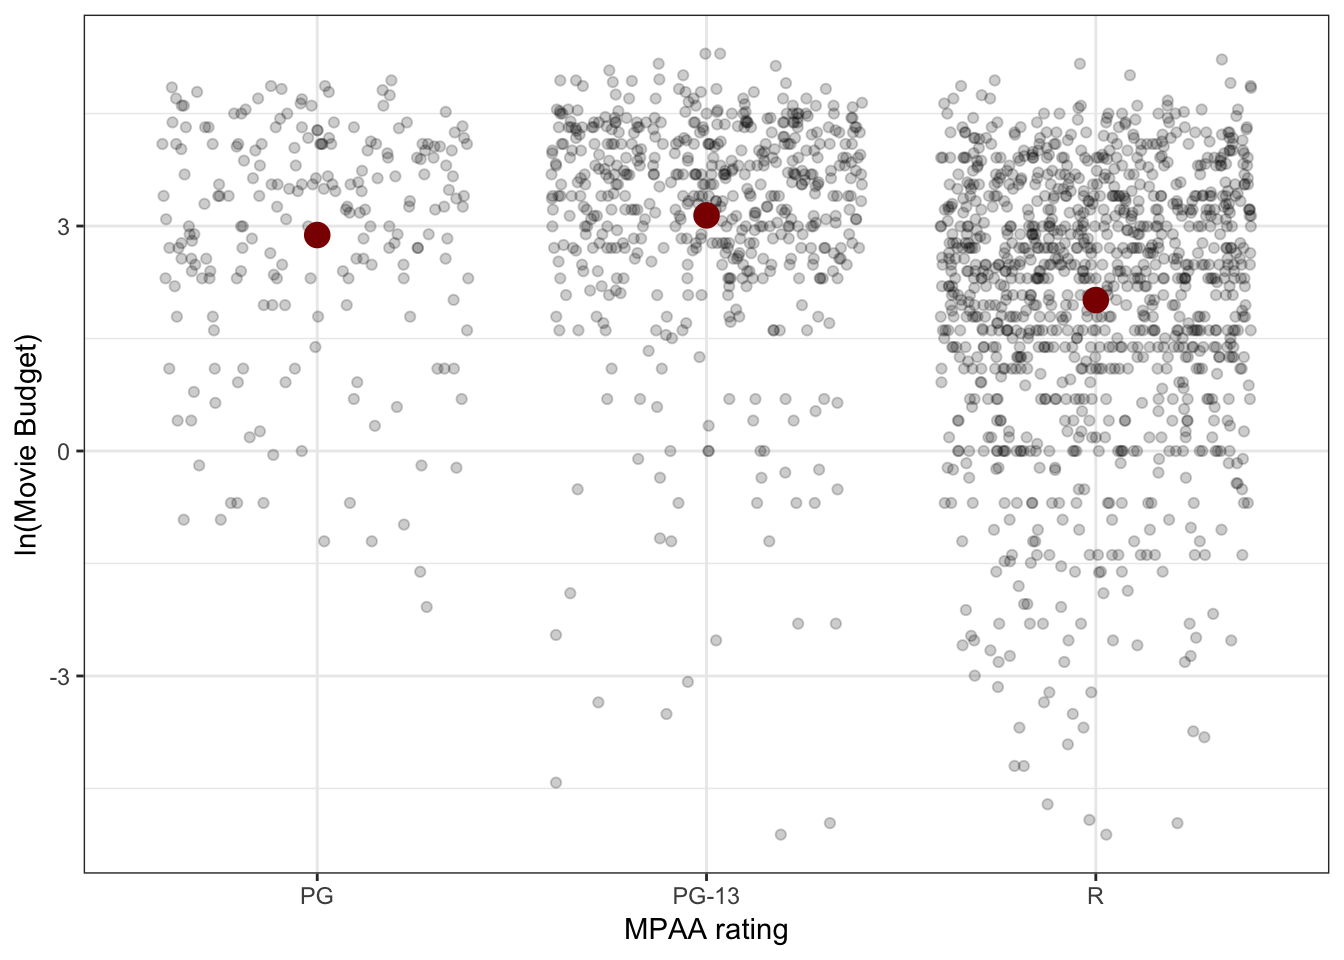
\includegraphics[width=0.5\linewidth]{epsy-8252-notes_files/figure-latex/unnamed-chunk-71-1} 

}

\caption{Jittered scatterplot of log-budget versus MPAA rating.}\label{fig:unnamed-chunk-71}
\end{figure}

\begin{Shaded}
\begin{Highlighting}[]
\CommentTok{# Compute summary statistics}
\NormalTok{movies }\OperatorTok
\StringTok{  }\KeywordTok{group_by}\NormalTok{(mpaa) }\OperatorTok
\StringTok{  }\KeywordTok{summarize}\NormalTok{(}
    \DataTypeTok{M =} \KeywordTok{mean}\NormalTok{(Lbudget), }
    \DataTypeTok{SD =} \KeywordTok{sd}\NormalTok{(Lbudget)}
\NormalTok{    )}
\end{Highlighting}
\end{Shaded}

\begin{verbatim}
# A tibble: 3 x 3
  mpaa      M    SD
  <chr> <dbl> <dbl>
1 PG     2.88  1.53
2 PG-13  3.14  1.51
3 R      2.01  1.78
\end{verbatim}

The scatterplot and summary statistics indicate there are sample differences in the mean log-budgets for the three MPAA ratings. The variation in log-budgets seems roughly the same for the three ratings.

\hypertarget{regression-model}{%
\subsection{Regression Model}\label{regression-model}}

Let's regress log-transformed budget on MPAA rating and examine the output from the model. To do so, we will need to first create three dummy variables for the different ratings.

\begin{Shaded}
\begin{Highlighting}[]
\CommentTok{# Create dummy variables}
\NormalTok{movies =}\StringTok{ }\NormalTok{movies }\OperatorTok
\StringTok{  }\KeywordTok{mutate}\NormalTok{(}
    \DataTypeTok{pg   =} \KeywordTok{if_else}\NormalTok{(mpaa }\OperatorTok{==}\StringTok{ "PG"}\NormalTok{, }\DecValTok{1}\NormalTok{, }\DecValTok{0}\NormalTok{),}
    \DataTypeTok{pg13 =} \KeywordTok{if_else}\NormalTok{(mpaa }\OperatorTok{==}\StringTok{ "PG-13"}\NormalTok{, }\DecValTok{1}\NormalTok{, }\DecValTok{0}\NormalTok{),}
    \DataTypeTok{r    =} \KeywordTok{if_else}\NormalTok{(mpaa }\OperatorTok{==}\StringTok{ "R"}\NormalTok{, }\DecValTok{1}\NormalTok{, }\DecValTok{0}\NormalTok{)}
\NormalTok{  )}

\CommentTok{# Fit the model (pg is reference group)}
\NormalTok{lm}\FloatTok{.3}\NormalTok{ =}\StringTok{ }\KeywordTok{lm}\NormalTok{(Lbudget }\OperatorTok{~}\StringTok{ }\DecValTok{1} \OperatorTok{+}\StringTok{ }\NormalTok{pg13 }\OperatorTok{+}\StringTok{ }\NormalTok{r, }\DataTypeTok{data =}\NormalTok{ movies)}

\CommentTok{# Model-level output}
\KeywordTok{glance}\NormalTok{(lm}\FloatTok{.3}\NormalTok{)}
\end{Highlighting}
\end{Shaded}

\begin{verbatim}
# A tibble: 1 x 11
  r.squared adj.r.squared sigma statistic  p.value    df logLik   AIC   BIC
      <dbl>         <dbl> <dbl>     <dbl>    <dbl> <int>  <dbl> <dbl> <dbl>
1    0.0892        0.0882  1.68      88.3 2.66e-37     3 -3495. 6997. 7019.
# ... with 2 more variables: deviance <dbl>, df.residual <int>
\end{verbatim}

The model-level summary information suggests that differences in MPAA rating explains 8.9\% of the variation in budget. (Remember, explaining variation in log-budget is the same as explaining variation in budget). Although this is a small amount of variation, it is statistically significant, \(F(2,1803)=88.28\), \(p<0.001\).

\begin{Shaded}
\begin{Highlighting}[]
\CommentTok{# Coefficient-level output}
\KeywordTok{tidy}\NormalTok{(lm}\FloatTok{.3}\NormalTok{)}
\end{Highlighting}
\end{Shaded}

\begin{verbatim}
# A tibble: 3 x 5
  term        estimate std.error statistic   p.value
  <chr>          <dbl>     <dbl>     <dbl>     <dbl>
1 (Intercept)    2.88      0.115     25.0  9.98e-119
2 pg13           0.262     0.136      1.92 5.45e-  2
3 r             -0.867     0.126     -6.88 8.49e- 12
\end{verbatim}

From the coefficient-level output we see that the fitted equation is:

\[
\ln\left(\hat{\mathrm{Budget}_i}\right) = 2.88 + 0.26(\mathrm{PG\mbox{-}13}_i) - 0.87(\mathrm{R}_i)
\]

With log-transformations, there are two possible interpretations we can offer. The first is to interpret the coefficients using the log-transformed values. These we interpret in the exact same way we do any other regression coefficients (except we use log-outcome instead of outcome):

\begin{itemize}
\tightlist
\item
  The intercept, \(\hat{\beta_0} = 2.88\), is the average predicted log-budget for PG rated movies.
\item
  The slope associated with PG-13, \(\hat{\beta_1} = 0.26\), indicates that PG-13 rated movies have a log-budget that is 0.26 higher than PG rated movies, on average.
\item
  The slope associated with R, \(\hat{\beta_2} = -0.87\), indicates that R rated movies have a log-budget that is 0.87 lower than PG rated movies, on average.
\end{itemize}

We can also interpret these by back-transforming to raw budget. To do that we exponentiate the coefficients.

\begin{Shaded}
\begin{Highlighting}[]
\KeywordTok{exp}\NormalTok{(}\KeywordTok{coef}\NormalTok{(lm}\FloatTok{.3}\NormalTok{))}
\end{Highlighting}
\end{Shaded}

\begin{verbatim}
(Intercept)        pg13           r 
    17.8134      1.2998      0.4201 
\end{verbatim}

\begin{itemize}
\tightlist
\item
  PG rated movies have a budget of 17.81 million dollars, on average.
\item
  PG-13 rated movies have a budget that is 1.30 TIMES the estimated budget for PG rated movies, on average.
\item
  R rated movies have a budget that is 0.42 TIMES the estimated budget for PG rated movies, on average.
\end{itemize}

\hypertarget{mathematical-explanation-1}{%
\subsection{Mathematical Explanation}\label{mathematical-explanation-1}}

Remember, if we want to interpret using the raw metric of \(Y\), we need to back-transform from \(\ln(Y)\) to \(Y\). To back-transform, we use the inverse function, which is to exponentiate using the base of the logarithm, in our case, base-\(e\). For our example, when we exponentiate both sides of the fitted equation:

\[
\begin{split}
e^{\ln\left(\hat{\mathrm{Budget}_i}\right)} &= e^{2.88 + 0.26(\mathrm{PG\mbox{-}13}_i) - 0.87(\mathrm{R}_i)} \\
\hat{\mathrm{Budget}_i} &= e^{2.88} \times e^{0.26(\mathrm{PG\mbox{-}13}_i)} \times e^{-0.87(\mathrm{R}_i)}
\end{split}
\]

To interpret the effects (which are now interpreted using budget---not log-budget) we can substitute in the different dummy variable patterns and solve.

\[
\begin{split}
\textbf{PG Movie:}~~ \hat{\mathrm{Budget}_i} &= e^{2.88} \times e^{0.26(0)} \times e^{-0.87(0)}\\
&= 17.81 \times 1 \times 1 \\
&= 17.81
\end{split}
\]

\[
\begin{split}
\textbf{PG-13 Movie:}~~ \hat{\mathrm{Budget}_i} &= e^{2.88} \times e^{0.26(1)} \times e^{-0.87(0)}\\
&= 17.81 \times 1.30 \times 1 \\
&= 23.15
\end{split}
\]

\[
\begin{split}
\textbf{R Movie:}~~ \hat{\mathrm{Budget}_i} &= e^{2.88} \times e^{0.26(0)} \times e^{-0.87(1)}\\
&= 17.81 \times 1 \times 0.42 \\
&= 7.48
\end{split}
\]

\hypertarget{approximate-interpretations}{%
\subsection{Approximate Interpretations}\label{approximate-interpretations}}

Unfortunately, the approximate interpretations of the slopes by directly interpreting the coefficients using the language of percent change are not completely trustworthy. If we did interpret them, the interpretations for the two slopes would be:

\begin{itemize}
\tightlist
\item
  PG-13 rated movies have budget that is 26.2 percent higher than PG rated movies, on average.
\item
  R rated movies have budget that is 87 percent lower than PG rated movies, on average.
\end{itemize}

This interpretation is roughly true for the PG-13 effect, but not for the R effect. This approximate interpretation starts to become untrustworthy when the slope value is higher than about 0.20 or so.

\hypertarget{multiple-regression-main-effects-model}{%
\section{Multiple Regression: Main Effects Model}\label{multiple-regression-main-effects-model}}

Now we can fit a model that includes our focal predictor of age and our covariate of MPAA rating.

\begin{Shaded}
\begin{Highlighting}[]
\CommentTok{# Fit model (PG is reference group)}
\NormalTok{lm}\FloatTok{.4}\NormalTok{ =}\StringTok{ }\KeywordTok{lm}\NormalTok{(Lbudget }\OperatorTok{~}\StringTok{ }\DecValTok{1} \OperatorTok{+}\StringTok{ }\NormalTok{age }\OperatorTok{+}\StringTok{ }\NormalTok{pg13 }\OperatorTok{+}\StringTok{ }\NormalTok{r, }\DataTypeTok{data =}\NormalTok{ movies)}

\CommentTok{# Model-level output}
\KeywordTok{glance}\NormalTok{(lm}\FloatTok{.4}\NormalTok{)}
\end{Highlighting}
\end{Shaded}

\begin{verbatim}
# A tibble: 1 x 11
  r.squared adj.r.squared sigma statistic  p.value    df logLik   AIC   BIC
      <dbl>         <dbl> <dbl>     <dbl>    <dbl> <int>  <dbl> <dbl> <dbl>
1     0.109         0.108  1.66      73.8 4.82e-45     4 -3474. 6959. 6986.
# ... with 2 more variables: deviance <dbl>, df.residual <int>
\end{verbatim}

The model-level summary information suggests that differences in age and MPAA rating of a movie explains 11.0\% of the variation in budget. (Remember, explaining variation in log-budget is the same as explaining variation in budget); \(F(3,1802)=73.84\), \(p<0.001\).

\begin{Shaded}
\begin{Highlighting}[]
\CommentTok{# Coefficient-level output}
\KeywordTok{tidy}\NormalTok{(lm}\FloatTok{.4}\NormalTok{)}
\end{Highlighting}
\end{Shaded}

\begin{verbatim}
# A tibble: 4 x 5
  term        estimate std.error statistic  p.value
  <chr>          <dbl>     <dbl>     <dbl>    <dbl>
1 (Intercept)   3.73     0.175       21.3  3.76e-90
2 age          -0.0431   0.00673     -6.41 1.89e-10
3 pg13          0.208    0.135        1.54 1.23e- 1
4 r            -0.904    0.125       -7.24 6.79e-13
\end{verbatim}

The coefficient-level output suggest that there is still a statistically significant effect of age on budget, after controlling for differences in MPAA rating; \(t(1802)=-6.41\), \(p<.001\).

To determine if there is an effect of MPAA rating, after accounting for differences in age, at least one of the effects of MPAA rating need to be statistically significant. Here we see that the coefficient associated with rated R movies is statistically significant.

Remember that when we have more than two categories (more than one dummy variable) there can be many ways for the effect to play out, and not all of these are represented in the model we fitted. One way we can simultaneously examine ALL the ways this effect can play out is to use a nested \(F\)-test.

\hypertarget{nested-f-test}{%
\subsection{Nested F-Test}\label{nested-f-test}}

If we want to examine if there is a controlled effect of MPAA rating (controlling for age), we want to see whether by including MPAA rating in a model THAT ALREADY INCLUDES age we explain additional variation in the outcome. To do this we can compare a model that only includes the effect of age to a model that includes both the effects of age and MPAA rating. If the latter model explains a statistically significant amount of additional variation we can say that there is an effect of MPAA rating after controlling for differences in age.

In statistical hypothesis testing we are examining the following null hypothesis:

\[
H_0: \rho^2_{\mathrm{Age},\mathrm{MPAA~rating}} - \rho^2_{\mathrm{Age}} = 0
\]

If we fail to reject this hypothesis, then the two models explain the SAME amount of variation and we should adopt the simpler model; MPAA rating does not explain additional variation in budget. If we reject this hypothesis, MPAA rating does explain additional variation in budget, above and beyond age; and we should adopt the model that includes both effects.

To test this hypothesis we fit both models and then give both models to the \texttt{anova()} function.

\begin{Shaded}
\begin{Highlighting}[]
\CommentTok{# Fit models}
\NormalTok{lm}\FloatTok{.2}\NormalTok{ =}\StringTok{ }\KeywordTok{lm}\NormalTok{(Lbudget }\OperatorTok{~}\StringTok{ }\DecValTok{1} \OperatorTok{+}\StringTok{ }\NormalTok{age,            }\DataTypeTok{data =}\NormalTok{ movies)}
\NormalTok{lm}\FloatTok{.4}\NormalTok{ =}\StringTok{ }\KeywordTok{lm}\NormalTok{(Lbudget }\OperatorTok{~}\StringTok{ }\DecValTok{1} \OperatorTok{+}\StringTok{ }\NormalTok{age }\OperatorTok{+}\StringTok{ }\NormalTok{pg13 }\OperatorTok{+}\StringTok{ }\NormalTok{r, }\DataTypeTok{data =}\NormalTok{ movies)}

\CommentTok{# Nested F-test}
\KeywordTok{anova}\NormalTok{(lm}\FloatTok{.2}\NormalTok{, lm}\FloatTok{.4}\NormalTok{)}
\end{Highlighting}
\end{Shaded}

\begin{verbatim}
Analysis of Variance Table

Model 1: Lbudget ~ 1 + age
Model 2: Lbudget ~ 1 + age + pg13 + r
  Res.Df  RSS Df Sum of Sq    F Pr(>F)    
1   1804 5448                             
2   1802 4957  2       491 89.2 <2e-16 ***
---
Signif. codes:  0 '***' 0.001 '**' 0.01 '*' 0.05 '.' 0.1 ' ' 1
\end{verbatim}

The test suggests that there is a statistically significant effect of MPAA rating even after accounting for differences in age; \(F(2, 1802)=89.21\), \(p<.001\).

\hypertarget{coefficient-level-interpretation}{%
\subsection{Coefficient-Level Interpretation}\label{coefficient-level-interpretation}}

To interpret the coefficients, we will again exponentiate the fitted coefficients so we can interpret them using the raw-metric of budget.

\begin{Shaded}
\begin{Highlighting}[]
\KeywordTok{exp}\NormalTok{(}\KeywordTok{coef}\NormalTok{(lm}\FloatTok{.4}\NormalTok{))}
\end{Highlighting}
\end{Shaded}

\begin{verbatim}
(Intercept)         age        pg13           r 
    41.7120      0.9578      1.2318      0.4051 
\end{verbatim}

\begin{itemize}
\tightlist
\item
  The model estimated budget for a PG movie (reference group) that was made in 2019 (age = 0) is 41.71 million dollars.
\item
  Each one-year difference in age is associated with a 0.96-fold difference (4.3\% decrease) in budget, on average, controlling for differences in MPAA rating.
\item
  PG-13 rated movies have a budget that is 1.23 times that for PG movies, on average, controlling for differences in age.
\item
  R rated movies have a budget that is 0.41 times that for PG movies, on average, controlling for differences in age.
\end{itemize}

\hypertarget{plot-of-the-fitted-model}{%
\subsection{Plot of the Fitted Model}\label{plot-of-the-fitted-model}}

To plot the fitted model that includes a categorical predictor with more than two levels, it is best to re-fit the \texttt{lm()} using the categorical variable.

\begin{Shaded}
\begin{Highlighting}[]
\CommentTok{# Re-fit the model}
\NormalTok{lm}\FloatTok{.5}\NormalTok{ =}\StringTok{ }\KeywordTok{lm}\NormalTok{(Lbudget }\OperatorTok{~}\StringTok{ }\DecValTok{1} \OperatorTok{+}\StringTok{ }\NormalTok{age }\OperatorTok{+}\StringTok{ }\NormalTok{mpaa, }\DataTypeTok{data =}\NormalTok{ movies)}

\CommentTok{# Model-level output}
\KeywordTok{glance}\NormalTok{(lm}\FloatTok{.5}\NormalTok{)}
\end{Highlighting}
\end{Shaded}

\begin{verbatim}
# A tibble: 1 x 11
  r.squared adj.r.squared sigma statistic  p.value    df logLik   AIC   BIC
      <dbl>         <dbl> <dbl>     <dbl>    <dbl> <int>  <dbl> <dbl> <dbl>
1     0.109         0.108  1.66      73.8 4.82e-45     4 -3474. 6959. 6986.
# ... with 2 more variables: deviance <dbl>, df.residual <int>
\end{verbatim}

\begin{Shaded}
\begin{Highlighting}[]
\CommentTok{# Coefficient-level output}
\KeywordTok{tidy}\NormalTok{(lm}\FloatTok{.5}\NormalTok{)}
\end{Highlighting}
\end{Shaded}

\begin{verbatim}
# A tibble: 4 x 5
  term        estimate std.error statistic  p.value
  <chr>          <dbl>     <dbl>     <dbl>    <dbl>
1 (Intercept)   3.73     0.175       21.3  3.76e-90
2 age          -0.0431   0.00673     -6.41 1.89e-10
3 mpaaPG-13     0.208    0.135        1.54 1.23e- 1
4 mpaaR        -0.904    0.125       -7.24 6.79e-13
\end{verbatim}

Note this is the exact same model we fitted using the dummy variables, but R will choose the reference group for us (alphabetically). We can now set up our plotting data, predict, back-transform the outcome, and plot.

\begin{Shaded}
\begin{Highlighting}[]
\CommentTok{# Set up data}
\NormalTok{plot_data =}\StringTok{ }\KeywordTok{crossing}\NormalTok{(}
    \DataTypeTok{age =} \KeywordTok{seq}\NormalTok{(}\DataTypeTok{from =} \DecValTok{13}\NormalTok{, }\DataTypeTok{to =} \DecValTok{80}\NormalTok{, }\DataTypeTok{by =} \DecValTok{1}\NormalTok{),}
    \DataTypeTok{mpaa =} \KeywordTok{c}\NormalTok{(}\StringTok{"PG"}\NormalTok{, }\StringTok{"PG-13"}\NormalTok{, }\StringTok{"R"}\NormalTok{)}
\NormalTok{    ) }\OperatorTok
\StringTok{  }\KeywordTok{mutate}\NormalTok{(}
    \DataTypeTok{yhat =} \KeywordTok{predict}\NormalTok{(lm}\FloatTok{.5}\NormalTok{, }\DataTypeTok{newdata =}\NormalTok{ .),}
    \DataTypeTok{budget =} \KeywordTok{exp}\NormalTok{(yhat)}
\NormalTok{  )}

\CommentTok{# Examine data}
\KeywordTok{head}\NormalTok{(plot_data)}
\end{Highlighting}
\end{Shaded}

\begin{verbatim}
# A tibble: 6 x 4
    age mpaa   yhat budget
  <dbl> <chr> <dbl>  <dbl>
1    13 PG     3.17  23.8 
2    13 PG-13  3.38  29.3 
3    13 R      2.27   9.65
4    14 PG     3.13  22.8 
5    14 PG-13  3.34  28.1 
6    14 R      2.22   9.24
\end{verbatim}

\begin{Shaded}
\begin{Highlighting}[]
\CommentTok{# Plot}
\KeywordTok{ggplot}\NormalTok{(}\DataTypeTok{data =}\NormalTok{ plot_data, }\KeywordTok{aes}\NormalTok{(}\DataTypeTok{x =}\NormalTok{ age, }\DataTypeTok{y =}\NormalTok{ budget, }\DataTypeTok{color =}\NormalTok{ mpaa, }\DataTypeTok{linetype =}\NormalTok{ mpaa)) }\OperatorTok{+}
\StringTok{    }\KeywordTok{geom_line}\NormalTok{() }\OperatorTok{+}
\StringTok{    }\KeywordTok{theme_bw}\NormalTok{() }\OperatorTok{+}
\StringTok{  }\KeywordTok{xlab}\NormalTok{(}\StringTok{"Age"}\NormalTok{) }\OperatorTok{+}
\StringTok{  }\KeywordTok{ylab}\NormalTok{(}\StringTok{"Predicted budget (in millions of U.S. dollars)"}\NormalTok{) }\OperatorTok{+}
\StringTok{  }\NormalTok{ggsci}\OperatorTok{::}\KeywordTok{scale_color_d3}\NormalTok{(}\DataTypeTok{name =} \StringTok{"MPAA rating"}\NormalTok{) }\OperatorTok{+}
\StringTok{  }\KeywordTok{scale_linetype_manual}\NormalTok{(}\DataTypeTok{name =} \StringTok{"MPAA rating"}\NormalTok{, }\DataTypeTok{values =} \DecValTok{1}\OperatorTok{:}\DecValTok{3}\NormalTok{)}
\end{Highlighting}
\end{Shaded}

\begin{figure}

{\centering 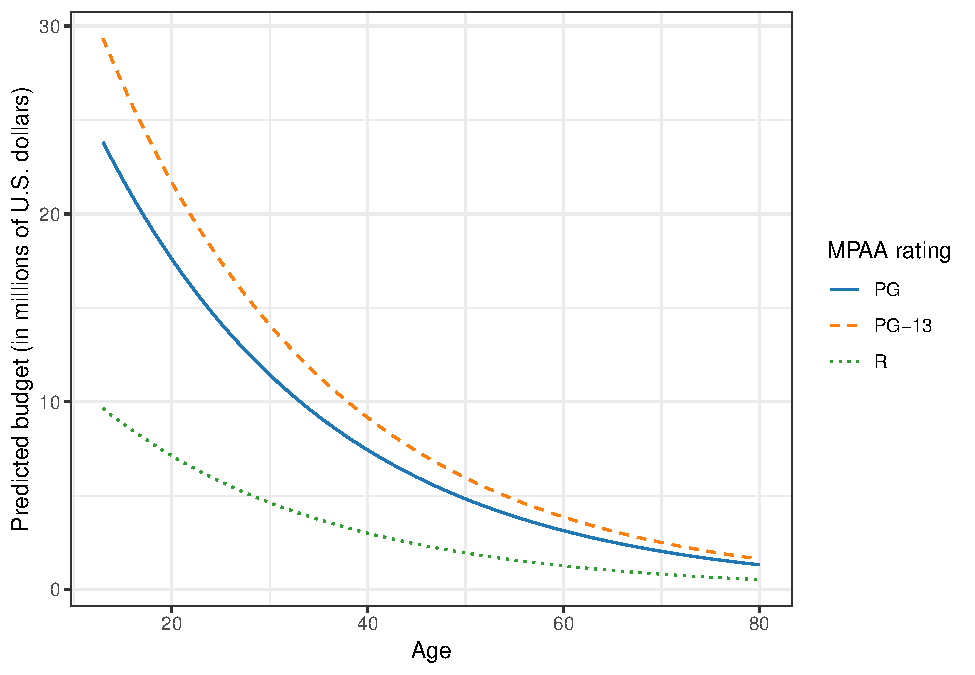
\includegraphics[width=0.5\linewidth]{epsy-8252-notes_files/figure-latex/unnamed-chunk-80-1} 

}

\caption{Plot of the predicted movie budget as a function of its age and MPAA rating. The non-linearity in the plot indicates that there is a diminishing negative effect of age on budget.}\label{fig:unnamed-chunk-80}
\end{figure}

The plot displays the negative, nonlinear effect of age on budget for all three types of movies (main effect of age). It also shows that PG-13 rated movies have a higher predicted budget than PG and R rated movies, and that PG rated movies have a higher predicted budget than R rated movies at EVERY age. This is the main effect of MPAA rating.

Notice that in the plot, the three lines are not parallel. This is a mathematical artifact of back-transforming log-budget to raw budget. It does not indicate that an interaction model was fitted. How non-parallel the lines are depends on the size of the coefficients associated with the MPAA effects (in this example). This is why, especially with transformed data, it is essential to plot the model to make sure you are understanding the interpretations from your coefficients.

\hypertarget{multiple-regression-interaction-model}{%
\section{Multiple Regression: Interaction Model}\label{multiple-regression-interaction-model}}

To study whether there is an interaction effect between MPAA rating and age, we will fit the interaction model and compare it to the main-effects model using the nested \(F\)-test.

\begin{Shaded}
\begin{Highlighting}[]
\CommentTok{# Fit the models}
\NormalTok{lm}\FloatTok{.5}\NormalTok{ =}\StringTok{ }\KeywordTok{lm}\NormalTok{(Lbudget }\OperatorTok{~}\StringTok{ }\DecValTok{1} \OperatorTok{+}\StringTok{ }\NormalTok{age }\OperatorTok{+}\StringTok{ }\NormalTok{mpaa,            }\DataTypeTok{data =}\NormalTok{ movies)}
\NormalTok{lm}\FloatTok{.6}\NormalTok{ =}\StringTok{ }\KeywordTok{lm}\NormalTok{(Lbudget }\OperatorTok{~}\StringTok{ }\DecValTok{1} \OperatorTok{+}\StringTok{ }\NormalTok{age }\OperatorTok{+}\StringTok{ }\NormalTok{mpaa }\OperatorTok{+}\StringTok{ }\NormalTok{age}\OperatorTok{:}\NormalTok{mpaa, }\DataTypeTok{data =}\NormalTok{ movies)}

\CommentTok{# Nested F-test}
\KeywordTok{anova}\NormalTok{(lm}\FloatTok{.5}\NormalTok{, lm}\FloatTok{.6}\NormalTok{)}
\end{Highlighting}
\end{Shaded}

\begin{verbatim}
Analysis of Variance Table

Model 1: Lbudget ~ 1 + age + mpaa
Model 2: Lbudget ~ 1 + age + mpaa + age:mpaa
  Res.Df  RSS Df Sum of Sq    F Pr(>F)
1   1802 4957                         
2   1800 4949  2      7.76 1.41   0.24
\end{verbatim}

The test suggests that we should adopt the main-effects model. The interaction-effect was not statistically significant; \(F(2,1800)=1.41\), \(p=.244\).

If the model that included the interaction effect was adopted, it would suggest that: (1) the effect of age on budget depends on MPAA rating, or (2) the effect of MPAA rating on budget depends on age of the movie. To further interpret these effects, you should plot the results of the fitted interaction model.

\hypertarget{log-transformations-some-final-thoughts}{%
\chapter*{Log Transformations: Some Final Thoughts}\label{log-transformations-some-final-thoughts}}
\addcontentsline{toc}{chapter}{Log Transformations: Some Final Thoughts}

There are four general curvilinear, monotonic functions (shown below).

\begin{figure}

{\centering 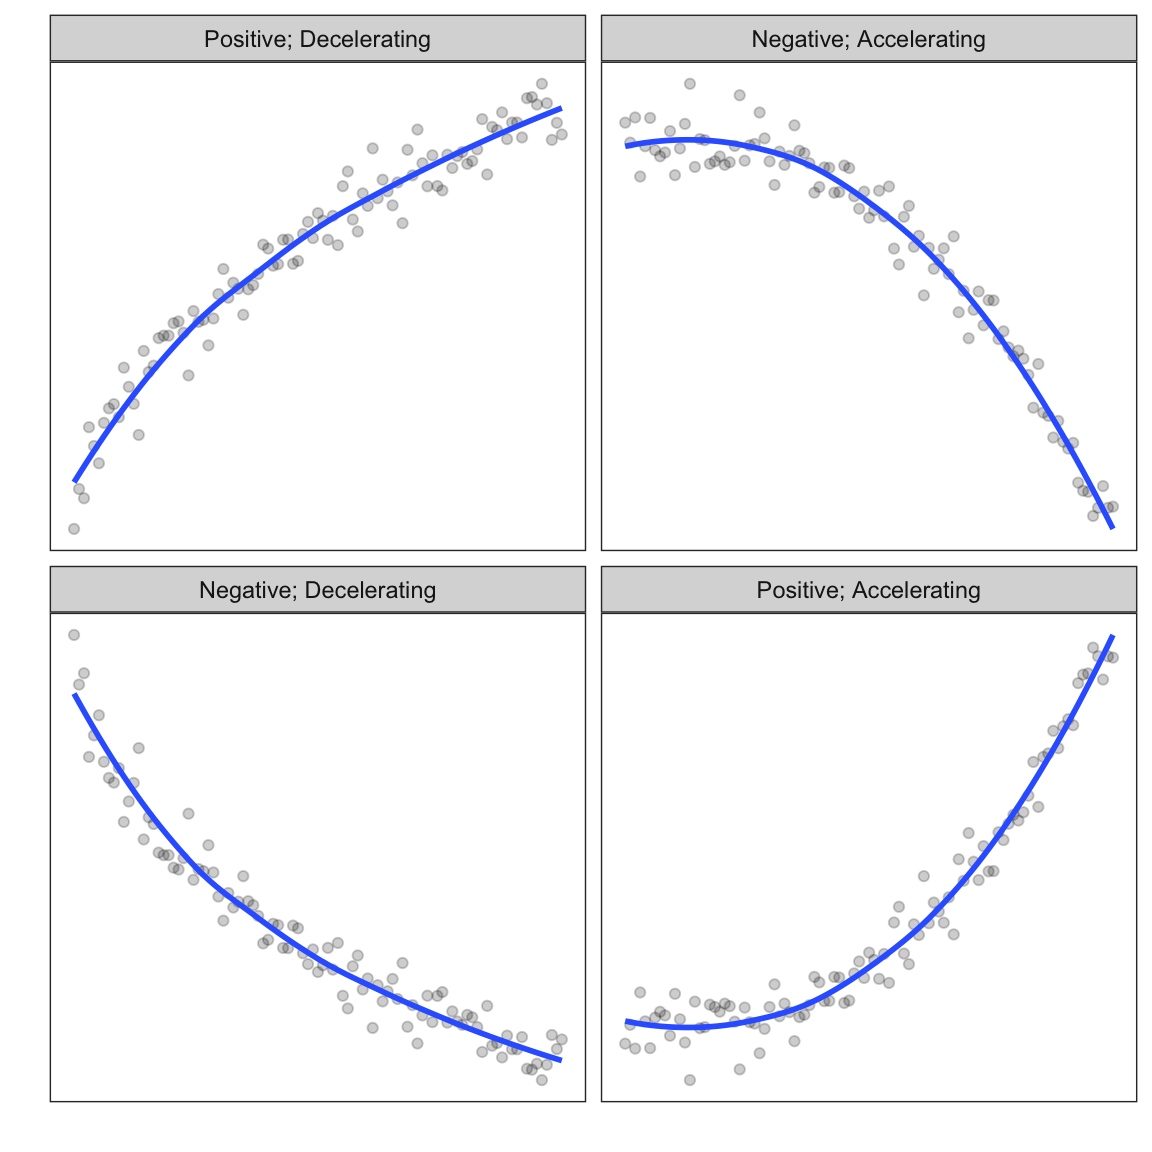
\includegraphics[width=0.8\linewidth]{epsy-8252-notes_files/figure-latex/unnamed-chunk-84-1} 

}

\caption{Four general monotonic, curvilinear shapes.}\label{fig:unnamed-chunk-84}
\end{figure}

In the previous two units you learned how to transform the data to ``linearize'' two of the four monotonic functions:

\begin{itemize}
\tightlist
\item
  For positive, decelerating functions we log-transformed \emph{X}; and
\item
  For positive, accelerating functions we log-transformed \emph{Y}.
\end{itemize}

To better understand how we can use transformations to straighten-out relationships, we will examine a set of transformations known as \textbf{power transformations}.

\hypertarget{power-transformations}{%
\section*{Power Transformations}\label{power-transformations}}
\addcontentsline{toc}{section}{Power Transformations}

Consider a set of powers, \(p\) that can be used in the exponent of a variable \(X\) (the variable is irrelevant; it could also be \(Y\)) so that a transformation of the variable \(X\) is:

\[
\mathrm{Transformed~Variable} = X^p
\]

Consider the following values for \(p\):

\[
p = \{-3,-2,-1,0,1,2,3\}
\]

These all represent particular transformations of \(X\). Note that when \(p=1\), the variable \(X\) is left untransformed (\(X^1 = X\)). Consider the following transformations:

\[
\begin{split}
&X^3 \\
&X^2 \\
&X^1 \qquad \mathrm{Untransformed}
\end{split}
\]

These are shown in the figure below.

\begin{center}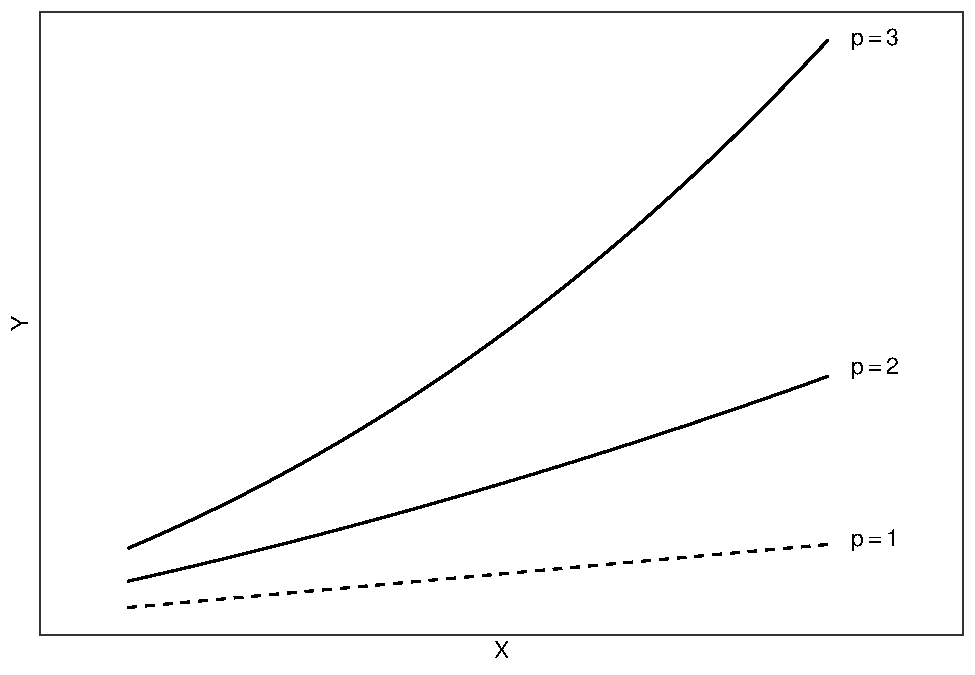
\includegraphics[width=0.5\linewidth]{epsy-8252-notes_files/figure-latex/unnamed-chunk-85-1} \end{center}

Power transformations that are bigger than 1 (\(p>1\)) show positive acceleration. Powers larger than one are referred to as \emph{upward} transformations as they increase the power (move it up) from one.

Now consider these transformations:

\[
\begin{split}
&X^{-1} \\
&X^{-2} \\
&X^{-3}
\end{split}
\]

These are shown in the figure below.

\begin{center}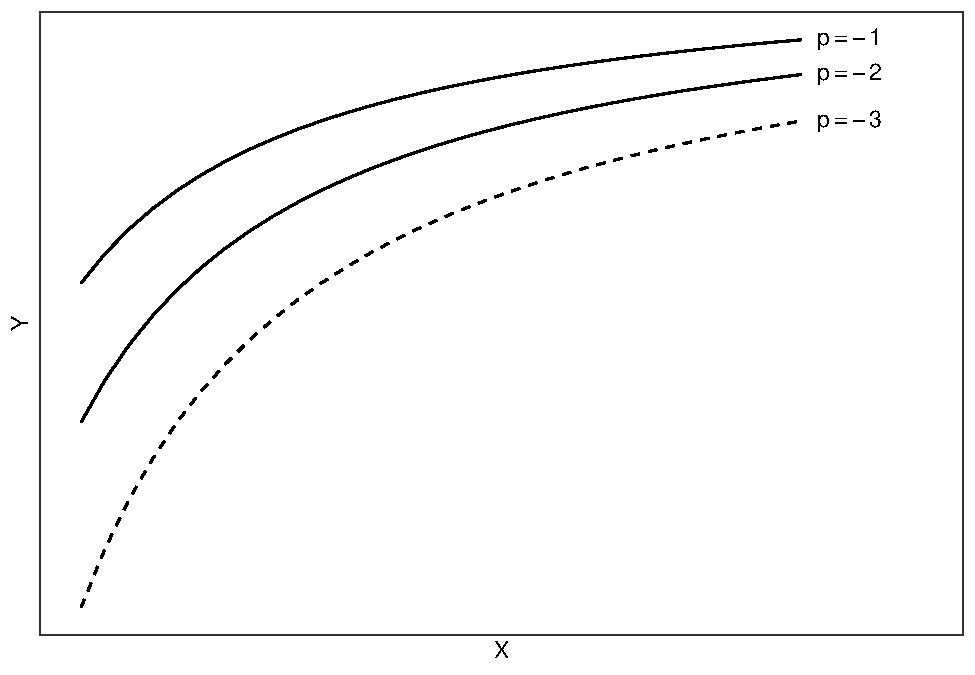
\includegraphics[width=0.5\linewidth]{epsy-8252-notes_files/figure-latex/unnamed-chunk-86-1} \end{center}

For power transformations that are smaller than 1 (\(p<1\)), the function shows positive deceleration. Powers that are smaller than one are referred to as \emph{downward} transformations as they decrease the power (move it down) from one.

\hypertarget{ladder-of-transformations}{%
\subsection*{Ladder of Transformations}\label{ladder-of-transformations}}
\addcontentsline{toc}{subsection}{Ladder of Transformations}

If we order the different values of \(p\), they form what statisticians call a ``ladder of re-expression'' or ``ladder of transformations''.

\[
\begin{split}
& ~~~~~\vdots \\
&Y^3,X^3 &\qquad \mathrm{Upward~Transformation}\\
&Y^2,X^2 &\qquad \mathrm{Upward~Transformation}\\
&Y^1,X^1  &\qquad \mathrm{Untransformed} \\
&Y^{\frac{1}{2}},X^{\frac{1}{2}} &\qquad \mathrm{Downward~Transformation}\\
&Y^0,X^0 \equiv \ln(X) &\qquad \mathrm{Downward~Transformation}\\
&Y^{-1},X^{-1} &\qquad \mathrm{Downward~Transformation}\\
&Y^{-2},X^{-2} &\qquad \mathrm{Downward~Transformation}\\
&Y^{-3},X^{-3} &\qquad \mathrm{Downward~Transformation} \\
& ~~~~~\vdots
\end{split}
\]

\hypertarget{rule-of-the-bulge}{%
\subsection*{Rule of the Bulge}\label{rule-of-the-bulge}}
\addcontentsline{toc}{subsection}{Rule of the Bulge}

To determine how we need to transform data, we can rely on Mosteller and Tukey's `Rule of the Bulge'. This rule, depicted visually below, has us ``move on the ladder in the direction in which the bulge points''.

\begin{figure}

{\centering 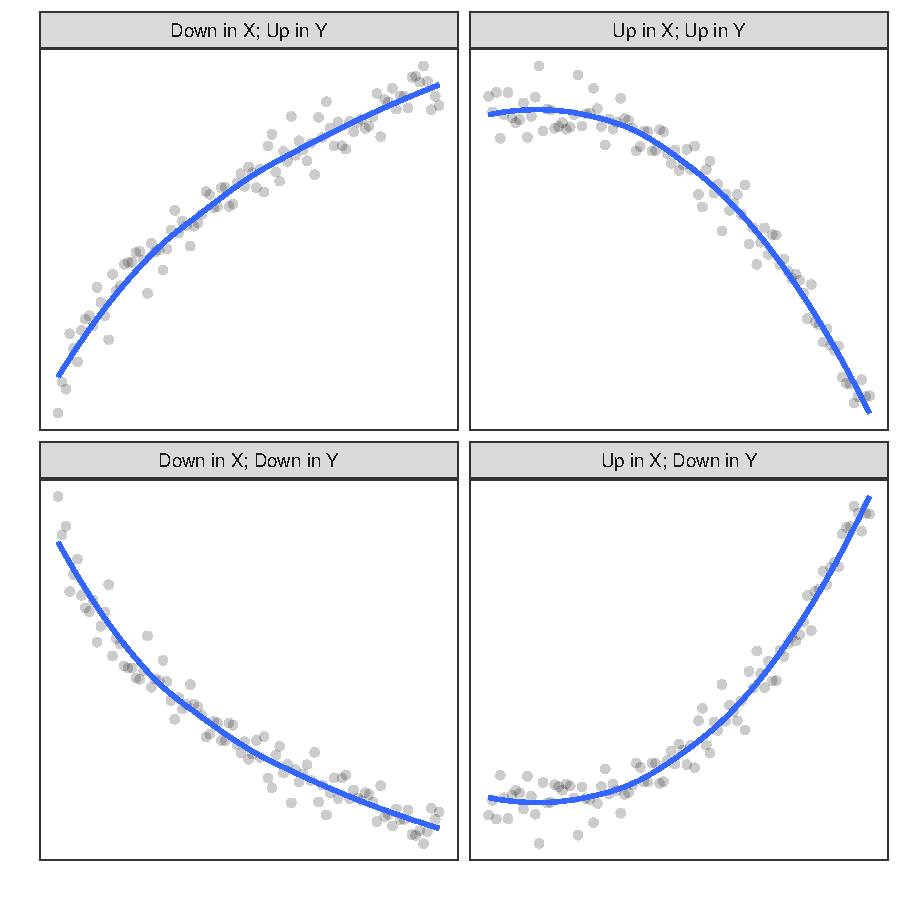
\includegraphics[width=0.8\linewidth]{epsy-8252-notes_files/figure-latex/unnamed-chunk-87-1} 

}

\caption{Four general monotonic, curvilinear shapes. The Rule of the Bulge helps us identify how to transform the data to linearize any of these four shapes.}\label{fig:unnamed-chunk-87}
\end{figure}

For example, below we re-visit the \texttt{mn-schools.csv} data and again look at the relationship between median SAT score and six-year graduation rate.

\begin{figure}

{\centering 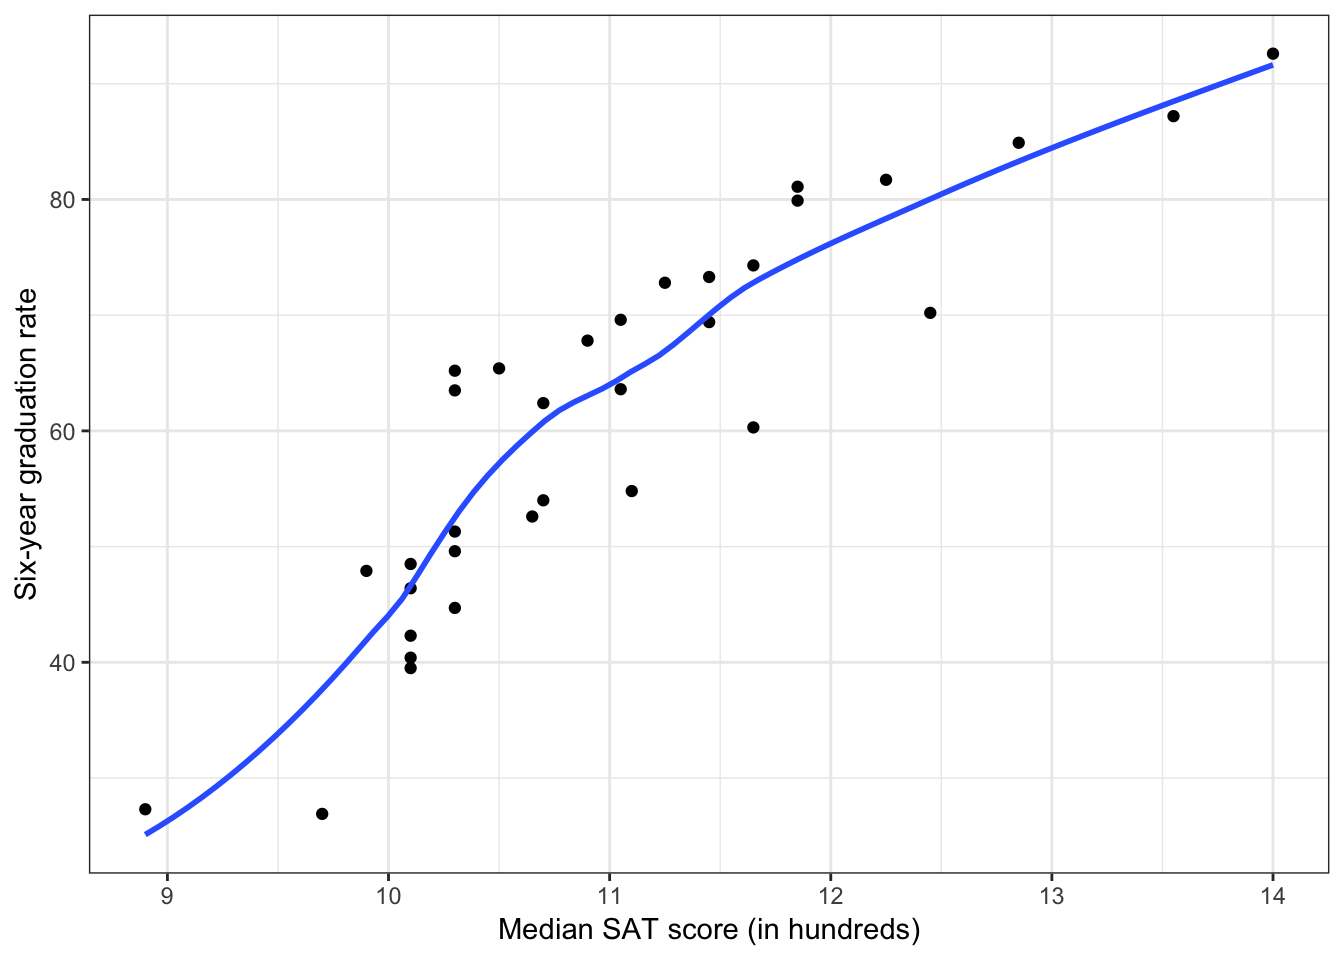
\includegraphics[width=0.5\linewidth]{epsy-8252-notes_files/figure-latex/unnamed-chunk-88-1} 

}

\caption{Scatterplot of the relationship between median SAT score and six-year graduation rate. The loess smoother is also displayed.}\label{fig:unnamed-chunk-88}
\end{figure}

This positive, decelerating relationship is similar to the one in the upper-lefthand quadrant of the `Rule of the Bulge'. To linearize this we can either:

\begin{itemize}
\tightlist
\item
  Transform \(X\) using a DOWNWARD transformation; or
\item
  Transform \(Y\) using an UPWARD transformation.
\end{itemize}

In the Unit 2 notes, we linearized this by taking the natural logarithm of SAT; a downward transformation of \(X\). What about the relationship between movie age and budget we looked at in Unit 3?

\begin{figure}

{\centering 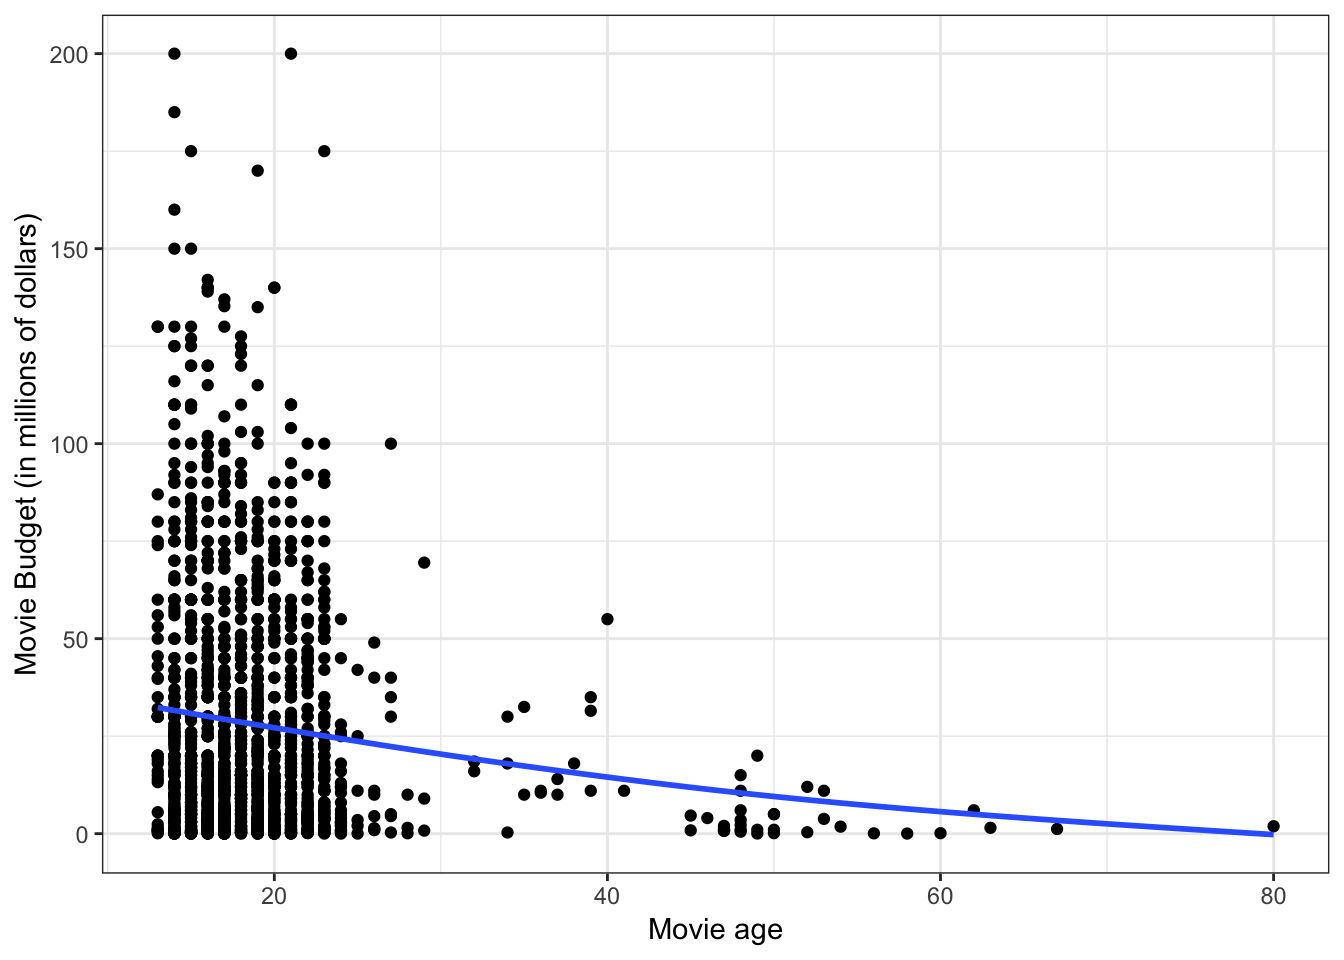
\includegraphics[width=0.5\linewidth]{epsy-8252-notes_files/figure-latex/unnamed-chunk-89-1} 

}

\caption{Scatterplot between age and budget. The loess smoother is also displayed.}\label{fig:unnamed-chunk-89}
\end{figure}

This negative, decelerating relationship is similar to the one in the lower-lefthand quadrant of the `Rule of the Bulge'. To linearize this we can either:

\begin{itemize}
\tightlist
\item
  Transform \(X\) using a DOWNWARD transformation; or
\item
  Transform \(Y\) using an DOWNWARD transformation.
\end{itemize}

In the Unit 3 notes, we linearized this by taking the natural logarithm of budget; a downward transformation of \(Y\). By transforming \(Y\) instead of \(X\), we also fixed a problem of heterogeneity of variance; a problem in the residuals (which is related to \(Y\)).

\hypertarget{probability-distributions}{%
\chapter{Probability Distributions}\label{probability-distributions}}

In this set of notes, you will learn about common probability distributions.

\begin{center}\rule{0.5\linewidth}{\linethickness}\end{center}

\hypertarget{preparation-3}{%
\subsection*{Preparation}\label{preparation-3}}
\addcontentsline{toc}{subsection}{Preparation}

Before class you will need to do the following:

\begin{itemize}
\item
  Read Section 3.1.1: Probability Basics in Fox {[}Required Textbook{]}
\item
  Read Sections 3.3.1--3.3.4 (Continuous Distributions) in Fox {[}Required Textbook{]}
\item
  Refresh your knowledge about probability distributions by going though the \href{https://www.khanacademy.org/math/probability/random-variables-topic}{Kahn Academy: Random Variables and Probability Distributions} tutorial.
\end{itemize}

\begin{center}\rule{0.5\linewidth}{\linethickness}\end{center}

\hypertarget{dataset-and-research-question-2}{%
\section{Dataset and Research Question}\label{dataset-and-research-question-2}}

In this set of notes, we will not be using a specific dataset.

\begin{Shaded}
\begin{Highlighting}[]
\CommentTok{# Load libraries}
\KeywordTok{library}\NormalTok{(broom)}
\KeywordTok{library}\NormalTok{(dplyr)}
\KeywordTok{library}\NormalTok{(ggplot2)}
\KeywordTok{library}\NormalTok{(readr)}
\KeywordTok{library}\NormalTok{(sm)}
\KeywordTok{library}\NormalTok{(tidyr)}
\end{Highlighting}
\end{Shaded}

\hypertarget{normal-distribution}{%
\section{Normal Distribution}\label{normal-distribution}}

The probability distribution of a normal distribution is mathematically defined as:

\[
p(x) = \frac{1}{\sigma\sqrt{2\pi}}\exp\left[-\frac{(x-\mu)^2}{2\sigma^2}\right]
\]

for \(-\infty \leq x \leq \infty\). Consider a normal distribution with a mean (\(\mu\)) of 50, and a standard deviation (\(\sigma\)) of 10. We can compute the probability density (\(p(x)\)) for a particular \(x\) value by using this equation. For example, the probability density for \(x=65\) can be found using,

\[
p(65) = \frac{1}{10\sqrt{2\pi}}\exp\left[-\frac{(65-50)^2}{2\times10^2}\right] = 0.01295176
\]

Using R, we can carry out the computation,

\begin{Shaded}
\begin{Highlighting}[]
\NormalTok{(}\DecValTok{1} \OperatorTok{/}\StringTok{ }\NormalTok{(}\DecValTok{10} \OperatorTok{*}\StringTok{ }\KeywordTok{sqrt}\NormalTok{(}\DecValTok{2} \OperatorTok{*}\StringTok{ }\NormalTok{pi))) }\OperatorTok{*}\StringTok{ }\KeywordTok{exp}\NormalTok{(}\OperatorTok{-}\NormalTok{(}\DecValTok{225}\NormalTok{) }\OperatorTok{/}\StringTok{ }\DecValTok{200}\NormalTok{)}
\end{Highlighting}
\end{Shaded}

\begin{verbatim}
[1] 0.01295
\end{verbatim}

There is also a more direct way to compute this using the \texttt{dnorm()} function. This function computes the density of \texttt{x} from a normal distribution with a specified \texttt{mean} and \texttt{sd}.

\begin{Shaded}
\begin{Highlighting}[]
\KeywordTok{dnorm}\NormalTok{(}\DataTypeTok{x =} \DecValTok{65}\NormalTok{, }\DataTypeTok{mean =} \DecValTok{50}\NormalTok{, }\DataTypeTok{sd =} \DecValTok{10}\NormalTok{)}
\end{Highlighting}
\end{Shaded}

\begin{verbatim}
[1] 0.01295
\end{verbatim}

If we compute the density for several \(x\) values and plot them, we get the familiar normal shape; the graphical depiction of the mathematical equation.

\begin{Shaded}
\begin{Highlighting}[]
\CommentTok{# Create dataset}
\NormalTok{fig_}\DecValTok{01}\NormalTok{ =}\StringTok{ }\KeywordTok{data.frame}\NormalTok{(}
  \DataTypeTok{X =} \KeywordTok{seq}\NormalTok{(}\DataTypeTok{from =} \DecValTok{10}\NormalTok{, }\DataTypeTok{to =} \DecValTok{90}\NormalTok{, }\DataTypeTok{by =} \FloatTok{0.01}\NormalTok{)}
\NormalTok{  ) }\OperatorTok\StringTok{ }
\StringTok{  }\KeywordTok{rowwise}\NormalTok{() }\OperatorTok
\StringTok{  }\KeywordTok{mutate}\NormalTok{(}
    \DataTypeTok{Y =} \KeywordTok{dnorm}\NormalTok{(}\DataTypeTok{x =}\NormalTok{ X, }\DataTypeTok{mean =} \DecValTok{50}\NormalTok{, }\DataTypeTok{sd =} \DecValTok{10}\NormalTok{)}
\NormalTok{    )}

\CommentTok{# Create plot}
\KeywordTok{ggplot}\NormalTok{(}\DataTypeTok{data =}\NormalTok{ fig_}\DecValTok{01}\NormalTok{, }\KeywordTok{aes}\NormalTok{(}\DataTypeTok{x =}\NormalTok{ X, }\DataTypeTok{y =}\NormalTok{ Y)) }\OperatorTok{+}
\StringTok{  }\KeywordTok{geom_line}\NormalTok{() }\OperatorTok{+}
\StringTok{  }\KeywordTok{theme_bw}\NormalTok{() }\OperatorTok{+}
\StringTok{  }\KeywordTok{geom_point}\NormalTok{(}\DataTypeTok{x =} \DecValTok{65}\NormalTok{, }\DataTypeTok{y =} \FloatTok{0.01295176}\NormalTok{, }\DataTypeTok{size =} \DecValTok{3}\NormalTok{)}
\end{Highlighting}
\end{Shaded}

\begin{figure}

{\centering 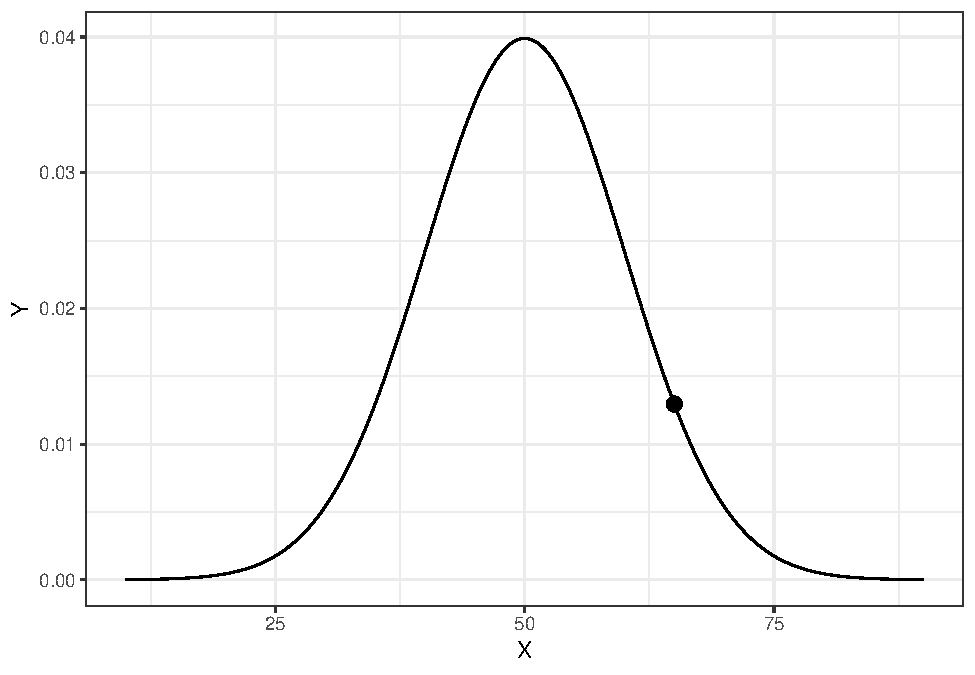
\includegraphics[width=0.5\linewidth]{epsy-8252-notes_files/figure-latex/unnamed-chunk-95-1} 

}

\caption{Plot of the probability density function (PDF) for a Normal distribution with mean of 50 and standard deviation of 10. The density value for $x=65$, $p(65)= 0.01295176$, is also displayed on the PDF.}\label{fig:unnamed-chunk-95}
\end{figure}

\hypertarget{other-useful-r-functions-for-working-with-probability-distributions}{%
\subsection{Other Useful R Functions for Working with Probability Distributions}\label{other-useful-r-functions-for-working-with-probability-distributions}}

There are four primary functions for working with the normal probability distribution:

\begin{itemize}
\tightlist
\item
  \texttt{dnorm()} : To compute the probability density (point on the curve)
\item
  \texttt{pnorm()} : To compute the probability (area under the PDF)
\item
  \texttt{qnorm()} : To compute the \(x\) value given a particular probability
\item
  \texttt{rnorm()} : To draw a random observation from the distribution
\end{itemize}

Each of these requires the arguments \texttt{mean=} and \texttt{sd=}. Let's look at some of them in use.

\hypertarget{finding-cumulative-probability}{%
\subsection{Finding Cumulative Probability}\label{finding-cumulative-probability}}

The function \texttt{pnorm()} gives the probability \(x\) is less than or equal to some quantile value in the distribution; the cumulative probability. For example, to find the probability that \(x \leq 65\) we would use,

\begin{Shaded}
\begin{Highlighting}[]
\KeywordTok{pnorm}\NormalTok{(}\DataTypeTok{q =} \DecValTok{65}\NormalTok{, }\DataTypeTok{mean =} \DecValTok{50}\NormalTok{, }\DataTypeTok{sd =} \DecValTok{10}\NormalTok{)}
\end{Highlighting}
\end{Shaded}

\begin{verbatim}
[1] 0.9332
\end{verbatim}

This is akin to finding the proportion of the area under the normal PDF that is to the left of 65.

\begin{figure}

{\centering 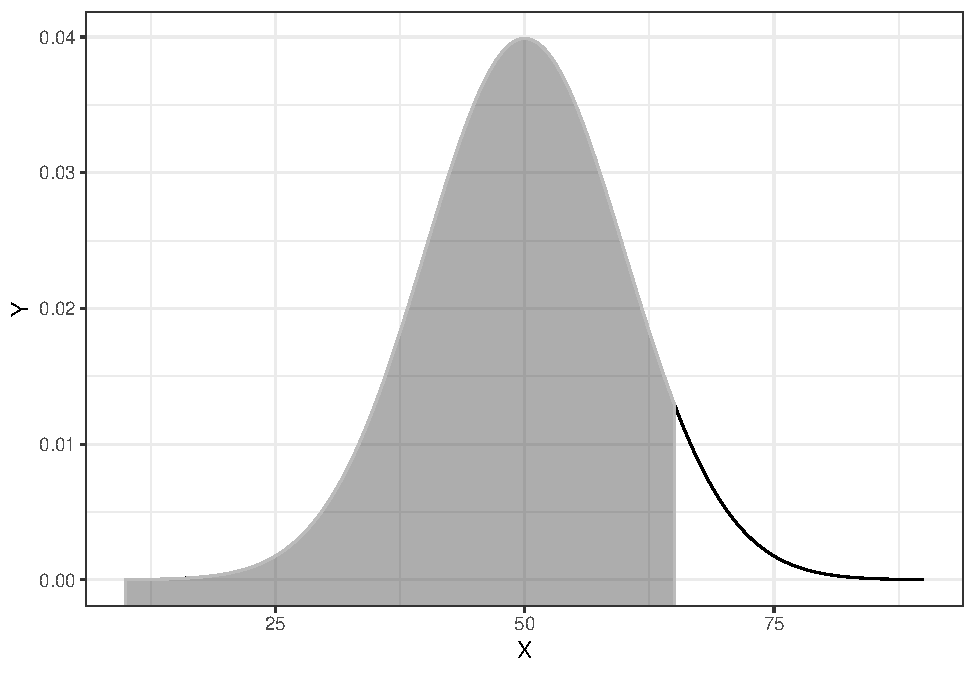
\includegraphics[width=0.5\linewidth]{epsy-8252-notes_files/figure-latex/unnamed-chunk-97-1} 

}

\caption{Plot of the PDF for a normal distribution (M=50, SD=10) with the cumulative probability for X less than or equal to 65 shaded.}\label{fig:unnamed-chunk-97}
\end{figure}

For the mathematically inclined, the grey-shaded area is expressed as an integral

\[
\int_{-\infty}^{65} p(x) dx
\]

where \(p(x)\) is the PDF for the normal distribution.

\hypertarget{cumulative-density-and-p-value}{%
\subsection{\texorpdfstring{Cumulative Density and \(p\)-Value}{Cumulative Density and p-Value}}\label{cumulative-density-and-p-value}}

This type of computation is used most commonly to find a \(p\)-value. The \(p\)-value is just the area under the distribution (curve) that is AT LEAST as extreme as some observed value. Consider a hypothesis test of whether a population parameter is equal to 0. Also consider that we observed a statistic (that has been standardized) of \(z=2.5\). Then, the \(p\)-value can be graphically displayed in the standard normal distribution as follows:

\begin{figure}

{\centering 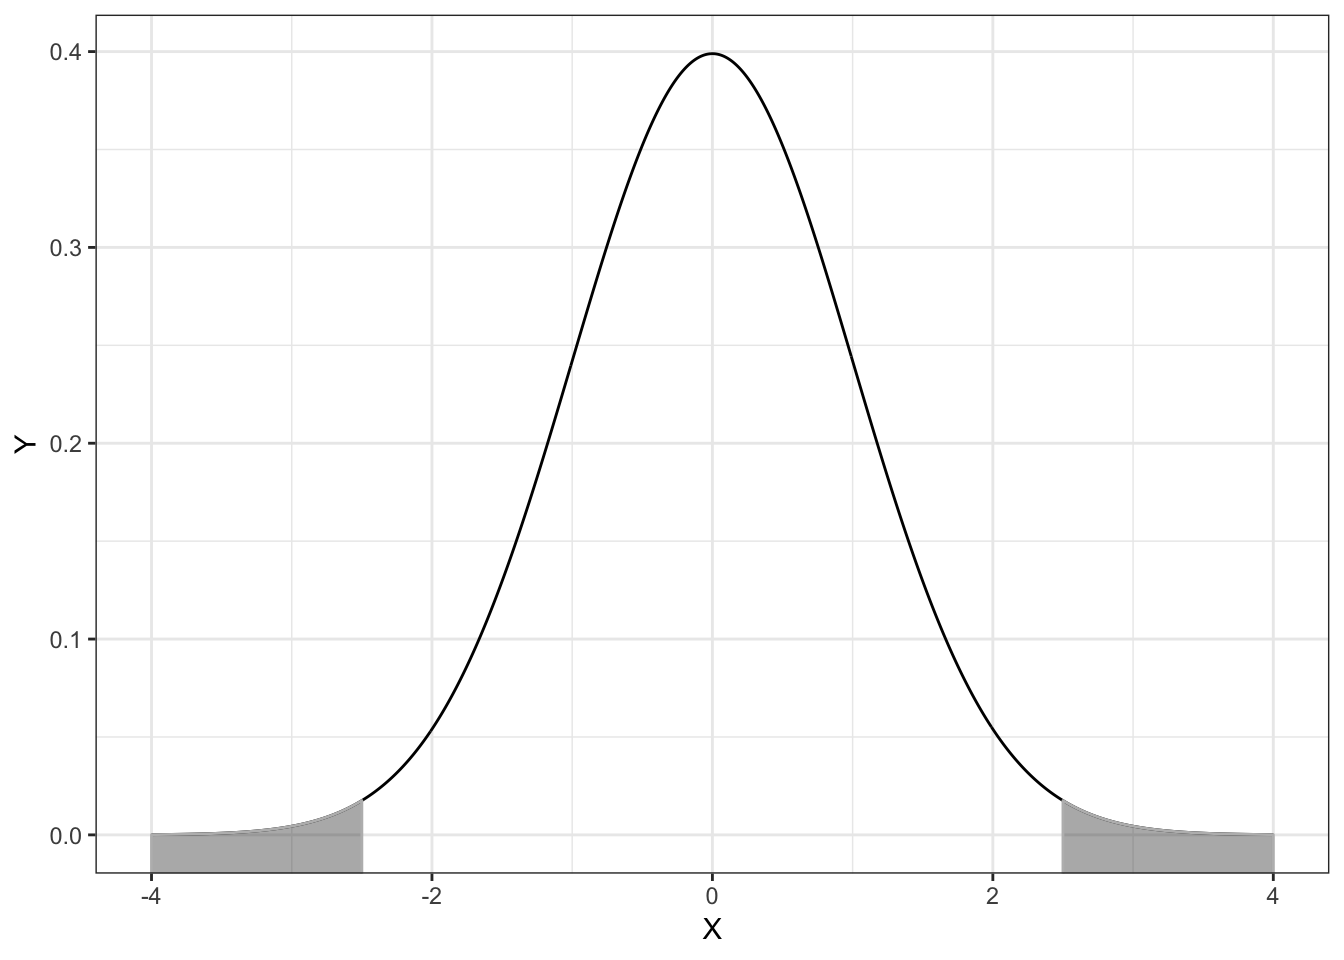
\includegraphics[width=0.5\linewidth]{epsy-8252-notes_files/figure-latex/unnamed-chunk-98-1} 

}

\caption{Plot of the probability density function (PDF) for the standard normal distribution (M=0, SD=1). The cumulative density representing the p-value for a two-tailed test evaluating whether mu=0 using an observed z-value of 2.5 is also displayed.}\label{fig:unnamed-chunk-98}
\end{figure}

In most hypothesis tests, we test whether the parameter IS EQUAL to 0. Thus the values in the standard normal distribution more extreme than 2.5 encompass evidence against the hypothesis; those values greater than 2.5 and also those values less than \(-2.5\). (This is akin to testing a fair coin when both 8 heads OR 8 tails would provide evidence against fairness \ldots we have to consider evidence in both directions).

To compute this we use \texttt{pnorm()}. Remember, it computes the proportion of the area under the curve TO THE LEFT of a particular value. Here we will compute the are to the left of \(-2.5\) and then double it to produce the actual \(p\)-value.

\begin{Shaded}
\begin{Highlighting}[]
\DecValTok{2} \OperatorTok{*}\StringTok{ }\KeywordTok{pnorm}\NormalTok{(}\DataTypeTok{q =} \FloatTok{-2.5}\NormalTok{, }\DataTypeTok{mean =} \DecValTok{0}\NormalTok{, }\DataTypeTok{sd =} \DecValTok{1}\NormalTok{)}
\end{Highlighting}
\end{Shaded}

\begin{verbatim}
[1] 0.01242
\end{verbatim}

\hypertarget{finding-quantiles}{%
\subsection{Finding Quantiles}\label{finding-quantiles}}

The \texttt{qnorm()} function is essentially the inverse of the \texttt{pnorm()} function. The \texttt{p} functions find the cumulative probability GIVEN a particular quantile. The \texttt{q} functions find the quantile GIVEN a cumulative probability. For example, in the normal distribution we defined earlier, half of the area is below the quantile value of 50 (the mean).

\begin{Shaded}
\begin{Highlighting}[]
\KeywordTok{qnorm}\NormalTok{(}\DataTypeTok{p =} \FloatTok{0.5}\NormalTok{, }\DataTypeTok{mean =} \DecValTok{50}\NormalTok{, }\DataTypeTok{sd =} \DecValTok{10}\NormalTok{)}
\end{Highlighting}
\end{Shaded}

\begin{verbatim}
[1] 50
\end{verbatim}

\hypertarget{students-t-distribution}{%
\section{\texorpdfstring{Student's \(t\)-Distribution}{Student's t-Distribution}}\label{students-t-distribution}}

Student's \(t\)-distribution looks like a standard normal distribution. In the figure below, Student's \(t\)-distribution is depicted with a solid, black line and the standard normal distribution (\(M=0\), \(SD=1\)) is depicted with a dotted, red line.

\begin{figure}

{\centering 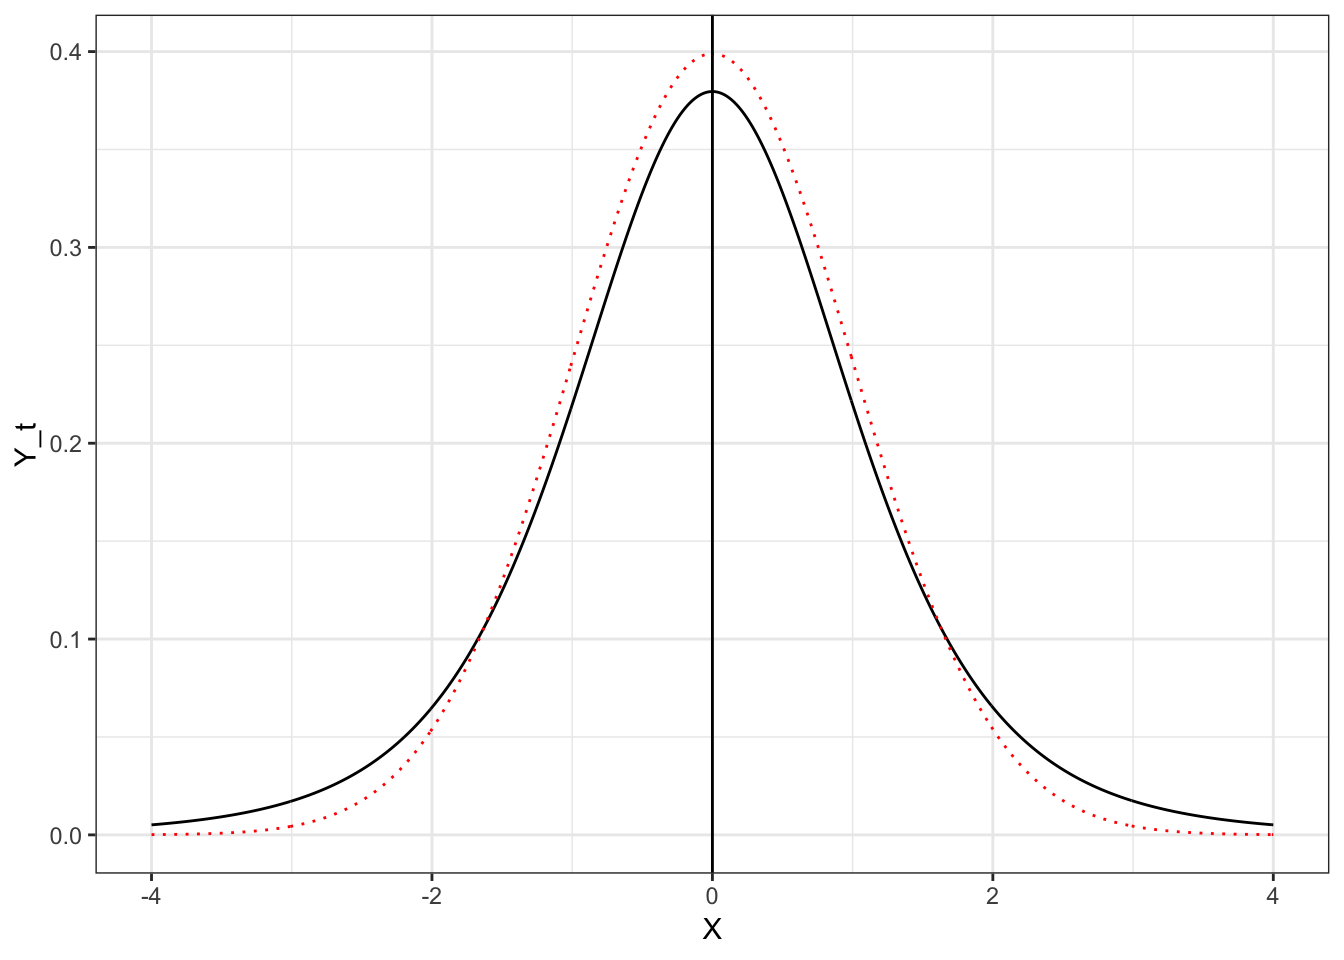
\includegraphics[width=0.5\linewidth]{epsy-8252-notes_files/figure-latex/unnamed-chunk-101-1} 

}

\caption{Plot of the probability density function (PDF) for the standard normal distribution (dotted, red line) and Student's t-distribution with 5 degrees of freedom (solid, black line).}\label{fig:unnamed-chunk-101}
\end{figure}

Both the standard normal distribution and Student's \(t\)-distribution have a mean (expected value) of 0. The standard deviation for Student's \(t\)-distribution is larger than the standard deviation for the standard normal distribution (\(SD>1\)). You can see this in the distribution because the tails in Student's \(t\)-distribution are fatter (more error) than the standard normal distribution.

In practice, we often use Student's \(t\)-distribution rather than the standard normal distribution when we are using sample data to estimate the population. This estimation increases the error and thus is typically modeled using Student's \(t\)-distribution.

Student's \(t\)-distribution constitutes a family of distributions---not just a single distribution. The specific shape (and thus probability density) is defined by the \emph{degrees of freedom}; \emph{df}. The plot below shows the standard normal distribution (purple) and four \(t\)-distributions with varying \emph{df}-values.

\begin{figure}

{\centering 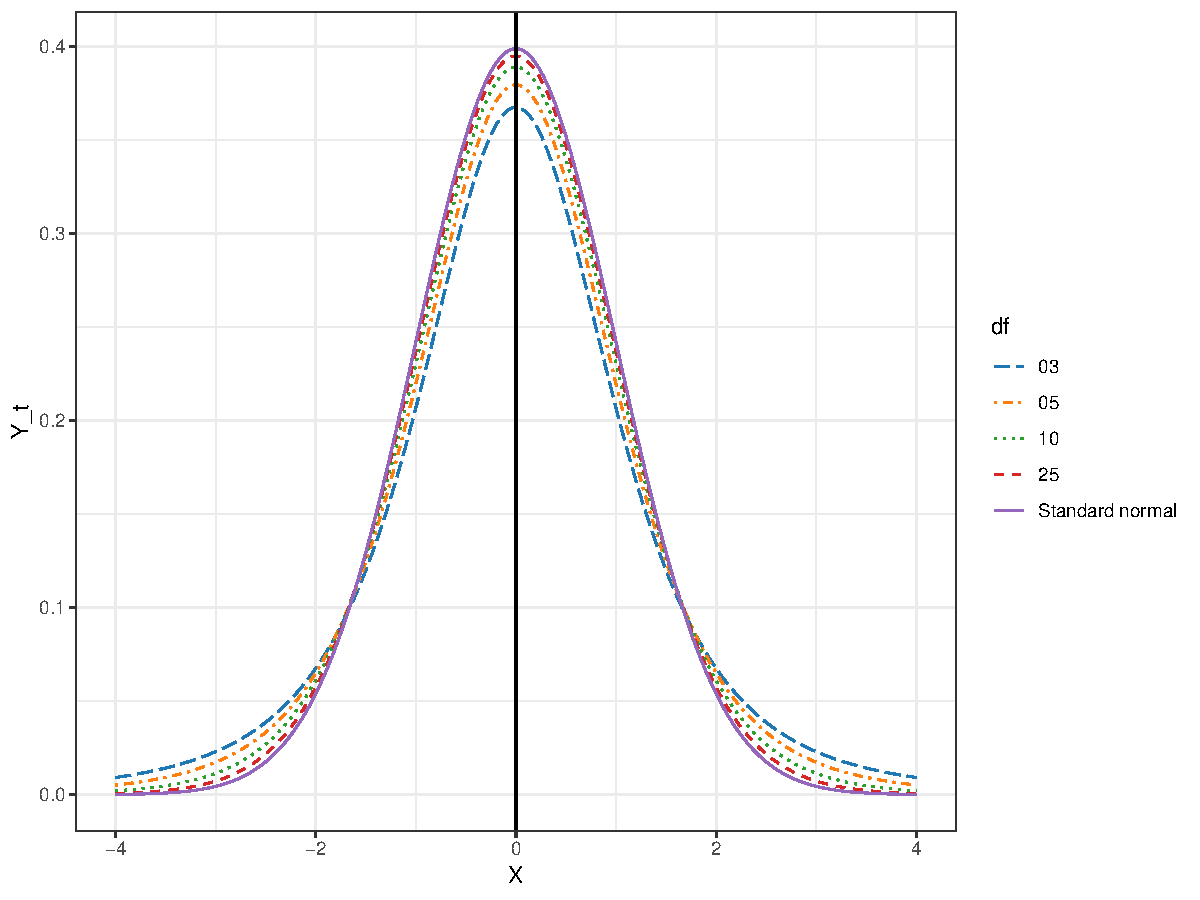
\includegraphics[width=0.8\linewidth]{epsy-8252-notes_files/figure-latex/unnamed-chunk-102-1} 

}

\caption{Plot of several t-distributions with differing degrees of freedom.}\label{fig:unnamed-chunk-102}
\end{figure}

\begin{verbatim}
  df M   SD
1 03 0 2.00
2 05 0 1.50
3 10 0 1.22
4 25 0 1.08
5  z 0 1.00
\end{verbatim}

If we compare the means and SDs for these distributions, we find that the mean for all the \(t\)-distributions is 0, same as the standard normal distribution. All \(t\)-distributions are unimodal and symmetric around zero. The SD for every \(t\)-distribution is higher than the SD for the standard normal distribution. Student \(t\)-distributions with higher \emph{df} values have less variation. It turns out that the standard normal distribution is a \(t\)-distribution with \(\infty\) \emph{df}. For the formula for the SD in a \(t\)-distribution, see \citet{Fox:2009}.

There are four primary functions for working with Student's \(t\)-distribution:

\begin{itemize}
\tightlist
\item
  \texttt{dt()} : To compute the probability density (point on the curve)
\item
  \texttt{pt()} : To compute the probability (area under the PDF)
\item
  \texttt{qt()} : To compute the \(x\) value given a particular probability
\item
  \texttt{rt()} : To draw a random observation from the distribution
\end{itemize}

Each of these requires the arguments \texttt{df=}. Let's look at some of them in use.

\hypertarget{comparing-probability-densities}{%
\subsection{Comparing Probability Densities}\label{comparing-probability-densities}}

How do the probability densities for a value of \(X\) compare across these distributions? Let's examine the \(X\) value of 2.

\begin{Shaded}
\begin{Highlighting}[]
\CommentTok{# Standard normal distribution}
\KeywordTok{pnorm}\NormalTok{(}\DataTypeTok{q =} \DecValTok{2}\NormalTok{, }\DataTypeTok{mean =} \DecValTok{0}\NormalTok{, }\DataTypeTok{sd =} \DecValTok{1}\NormalTok{)}
\end{Highlighting}
\end{Shaded}

\begin{verbatim}
[1] 0.9772
\end{verbatim}

\begin{Shaded}
\begin{Highlighting}[]
\CommentTok{# t-distribution with 3 df}
\KeywordTok{pt}\NormalTok{(}\DataTypeTok{q =} \DecValTok{2}\NormalTok{, }\DataTypeTok{df =} \DecValTok{3}\NormalTok{)}
\end{Highlighting}
\end{Shaded}

\begin{verbatim}
[1] 0.9303
\end{verbatim}

\begin{Shaded}
\begin{Highlighting}[]
\CommentTok{# t-distribution with 5 df}
\KeywordTok{pt}\NormalTok{(}\DataTypeTok{q =} \DecValTok{2}\NormalTok{, }\DataTypeTok{df =} \DecValTok{5}\NormalTok{)}
\end{Highlighting}
\end{Shaded}

\begin{verbatim}
[1] 0.949
\end{verbatim}

\begin{Shaded}
\begin{Highlighting}[]
\CommentTok{# t-distribution with 10 df}
\KeywordTok{pt}\NormalTok{(}\DataTypeTok{q =} \DecValTok{2}\NormalTok{, }\DataTypeTok{df =} \DecValTok{10}\NormalTok{)}
\end{Highlighting}
\end{Shaded}

\begin{verbatim}
[1] 0.9633
\end{verbatim}

\begin{Shaded}
\begin{Highlighting}[]
\CommentTok{# t-distribution with 25 df}
\KeywordTok{pt}\NormalTok{(}\DataTypeTok{q =} \DecValTok{2}\NormalTok{, }\DataTypeTok{df =} \DecValTok{25}\NormalTok{)}
\end{Highlighting}
\end{Shaded}

\begin{verbatim}
[1] 0.9718
\end{verbatim}

We are essentially comparing the height of these distributions at \(X=2\).

\begin{figure}

{\centering 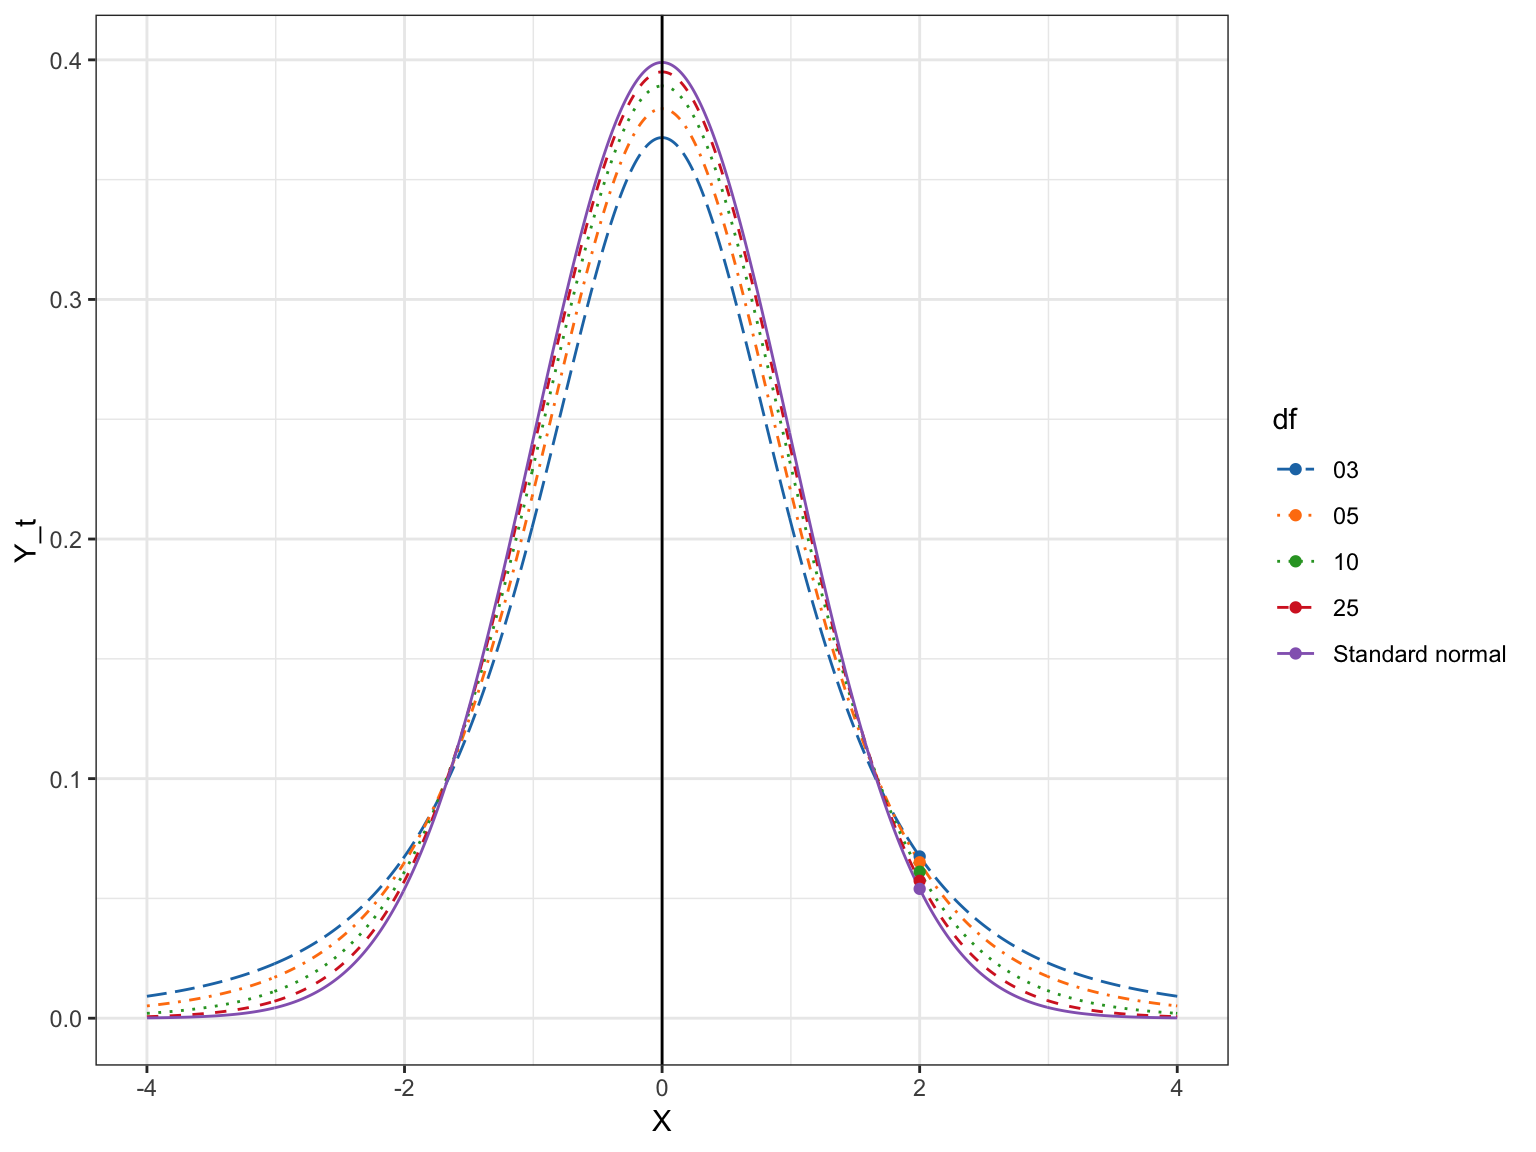
\includegraphics[width=0.8\linewidth]{epsy-8252-notes_files/figure-latex/unnamed-chunk-105-1} 

}

\caption{Plot of several t-distributions with differing *degrees of freedom. The probability density for t=2 is also displayed for each of the distributions.}\label{fig:unnamed-chunk-105}
\end{figure}

\hypertarget{comparing-cumulative-densities}{%
\subsection{Comparing Cumulative Densities}\label{comparing-cumulative-densities}}

What if we wanted to look at cumulative density? Consider out hypothesis test of whether a population parameter is equal to 0. Also consider that we observed a statistic (that has been standardized) of 2.5 using a sample size of \(n=15\).

If we can assume that the SAMPLING DISTRIBUTION is normally-distributed then we can use the cumulative density in a normal distribution to compute a \(p\)-value:

\begin{Shaded}
\begin{Highlighting}[]
\DecValTok{2} \OperatorTok{*}\StringTok{ }\KeywordTok{pnorm}\NormalTok{(}\DataTypeTok{q =} \FloatTok{-2.5}\NormalTok{, }\DataTypeTok{mean =} \DecValTok{0}\NormalTok{, }\DataTypeTok{sd =} \DecValTok{1}\NormalTok{)}
\end{Highlighting}
\end{Shaded}

\begin{verbatim}
[1] 0.01242
\end{verbatim}

If, however, the SAMPLING DISTRIBUTION is \(t\)-distributed then we need to use the cumulative density for a \(t\)-distribution with the appropriate \emph{df} to compute a \(p\)-value. For example if we use \(df=n-1\), the two-tailed \(p\)-value would be:

\begin{Shaded}
\begin{Highlighting}[]
\DecValTok{2} \OperatorTok{*}\StringTok{ }\KeywordTok{pt}\NormalTok{(}\DataTypeTok{q =} \FloatTok{-2.5}\NormalTok{, }\DataTypeTok{df =} \DecValTok{14}\NormalTok{)}
\end{Highlighting}
\end{Shaded}

\begin{verbatim}
[1] 0.02547
\end{verbatim}

The \(p\)-value using the \(t\)-distribution is larger than the \(p\)-value computed based on the standard normal distribution. This is again because of the increased error (uncertainty) we are introducing when we estimate from sample. This added uncertainty makes it harder for us to reject a hypothesis.

\hypertarget{using-the-t-distribution-in-regression}{%
\section{\texorpdfstring{Using the \(t\)-Distribution in Regression}{Using the t-Distribution in Regression}}\label{using-the-t-distribution-in-regression}}

To illustrate how probability distributions are used in practice, we will will use the \emph{riverview.csv} (see the \protect\hyperlink{riverview}{data codebook} here) and fit a regression model that uses education level and seniority to predict variation in employee income.

\begin{Shaded}
\begin{Highlighting}[]
\CommentTok{# Read in data}
\NormalTok{city =}\StringTok{ }\KeywordTok{read_csv}\NormalTok{(}\DataTypeTok{file =} \StringTok{"~/Documents/github/epsy-8252/data/riverview.csv"}\NormalTok{)}
\KeywordTok{head}\NormalTok{(city)}
\end{Highlighting}
\end{Shaded}

\begin{verbatim}
# A tibble: 6 x 6
  education income seniority gender  male party      
      <dbl>  <dbl>     <dbl> <chr>  <dbl> <chr>      
1         8  37449         7 male       1 Democrat   
2         8  26430         9 female     0 Independent
3        10  47034        14 male       1 Democrat   
4        10  34182        16 female     0 Independent
5        10  25479         1 female     0 Republican 
6        12  46488        11 female     0 Democrat   
\end{verbatim}

\begin{Shaded}
\begin{Highlighting}[]
\CommentTok{# Fit regression model}
\NormalTok{lm}\FloatTok{.1}\NormalTok{ =}\StringTok{ }\KeywordTok{lm}\NormalTok{(income }\OperatorTok{~}\StringTok{ }\DecValTok{1} \OperatorTok{+}\StringTok{ }\NormalTok{education }\OperatorTok{+}\StringTok{ }\NormalTok{seniority, }\DataTypeTok{data =}\NormalTok{ city)}

\CommentTok{# Coefficient-level output}
\KeywordTok{tidy}\NormalTok{(lm}\FloatTok{.1}\NormalTok{)}
\end{Highlighting}
\end{Shaded}

\begin{verbatim}
# A tibble: 3 x 5
  term        estimate std.error statistic     p.value
  <chr>          <dbl>     <dbl>     <dbl>       <dbl>
1 (Intercept)    6769.     5373.      1.26 0.218      
2 education      2252.      335.      6.73 0.000000220
3 seniority       739.      210.      3.52 0.00146    
\end{verbatim}

How do we obtain the \(p\)-value for each of the coefficients? Recall that the coefficients and SEs for the coefficients are computed directly from the raw data. Then we can compute a test-statistic by dividing the coefficient estimate by the SE. For example, to compute the test-statistic associated with education level:

\[
t = \frac{2252}{335} = 6.72
\]

Since we are estimating the SE using sample data, our test statistic is likely \(t\)-distributed. Which value should we use for \emph{df}? Well, for that, statistical theory tells us that we should use the error \emph{df} value. In our data,

\[
\begin{split}
n &= 32 \\
\mathrm{Total~df} &= 32-1 = 31\\
\mathrm{Model~df} &= 2~\mathrm{(two~predictors)} \\
\mathrm{Error~df} &= 31-2 = 29
\end{split}
\]

Using the \(t\)-distribution with 29 \emph{df},

\begin{Shaded}
\begin{Highlighting}[]
\DecValTok{2} \OperatorTok{*}\StringTok{ }\KeywordTok{pt}\NormalTok{(}\DataTypeTok{q =} \FloatTok{-6.72}\NormalTok{, }\DataTypeTok{df =} \DecValTok{29}\NormalTok{)}
\end{Highlighting}
\end{Shaded}

\begin{verbatim}
[1] 0.0000002257
\end{verbatim}

For seniority (and the intercept), we would use the same \(t\)-distribution, but our test statistic would differ:

\[
\begin{split}
t_{\mathrm{Intercept}} &= \frac{6769}{5373} = 1.26 \\
t_{\mathrm{Seniority}} &= \frac{739}{210} = 3.52 \\
\end{split}
\]

The associated \(p\)-values are:

\begin{Shaded}
\begin{Highlighting}[]
\CommentTok{# Intercept p-value}
\DecValTok{2} \OperatorTok{*}\StringTok{ }\KeywordTok{pt}\NormalTok{(}\DataTypeTok{q =} \FloatTok{-1.26}\NormalTok{, }\DataTypeTok{df =} \DecValTok{29}\NormalTok{)}
\end{Highlighting}
\end{Shaded}

\begin{verbatim}
[1] 0.2177
\end{verbatim}

\begin{Shaded}
\begin{Highlighting}[]
\CommentTok{# Seniority p-value}
\DecValTok{2} \OperatorTok{*}\StringTok{ }\KeywordTok{pt}\NormalTok{(}\DataTypeTok{q =} \FloatTok{-3.52}\NormalTok{, }\DataTypeTok{df =} \DecValTok{29}\NormalTok{)}
\end{Highlighting}
\end{Shaded}

\begin{verbatim}
[1] 0.001446
\end{verbatim}

\hypertarget{model-level-inference-the-f-distribution}{%
\section{\texorpdfstring{Model-Level Inference: The \(F\)-Distribution}{Model-Level Inference: The F-Distribution}}\label{model-level-inference-the-f-distribution}}

The model-level inference for regression is based on an \(F\)-statistic, which is a standardized measure of \(R^2\).

\begin{Shaded}
\begin{Highlighting}[]
\CommentTok{# Model-level output}
\KeywordTok{glance}\NormalTok{(lm}\FloatTok{.1}\NormalTok{)}
\end{Highlighting}
\end{Shaded}

\begin{verbatim}
# A tibble: 1 x 11
  r.squared adj.r.squared sigma statistic p.value    df logLik   AIC   BIC
      <dbl>         <dbl> <dbl>     <dbl>   <dbl> <int>  <dbl> <dbl> <dbl>
1     0.742         0.724 7646.      41.7 2.98e-9     3  -330.  668.  674.
# ... with 2 more variables: deviance <dbl>, df.residual <int>
\end{verbatim}

In this example, the sample \(R^2\) value is 0.742. Computation of the \(F\)-statistic relies on two \emph{df} values---the model degrees of freedom (2) and the error degrees of freedom (29). To compute the \(F\)-statistics from \(R^2\) we use:

\[
F = \frac{R^2}{1-R^2} \times \frac{\mathrm{df}_{\mathrm{Error}}}{\mathrm{df}_{\mathrm{Model}}}
\]

In our example, we compute \(F\) as:

\[
\begin{split}
F &= \frac{0.742}{1-0.742} \times \frac{29}{2} \\
&= 41.7
\end{split}
\]

We write this standardization of \(R^2\) as \(F(2,29)=41.7\).

\hypertarget{testing-the-model-level-null-hypothesis}{%
\subsection{Testing the Model-Level Null Hypothesis}\label{testing-the-model-level-null-hypothesis}}

It is often worth testing whether the model explains a statistically significant amount of variation in the population. To do this we test the null hypothesis:

\[
H_0:\rho^2 = 0
\]

Similar to the tests of the coefficients, we evaluate our test statistic (\(F\) in this case) in the appropriate test distribution, in this case an \(F\)-distribution with 2 and 29 degrees of freedom. (The shape of the \(F\)-distribution is based on two \emph{df} values.) The figure below, shows the \(F(2,29)\)-distribution as a solid, black line.

\begin{figure}

{\centering 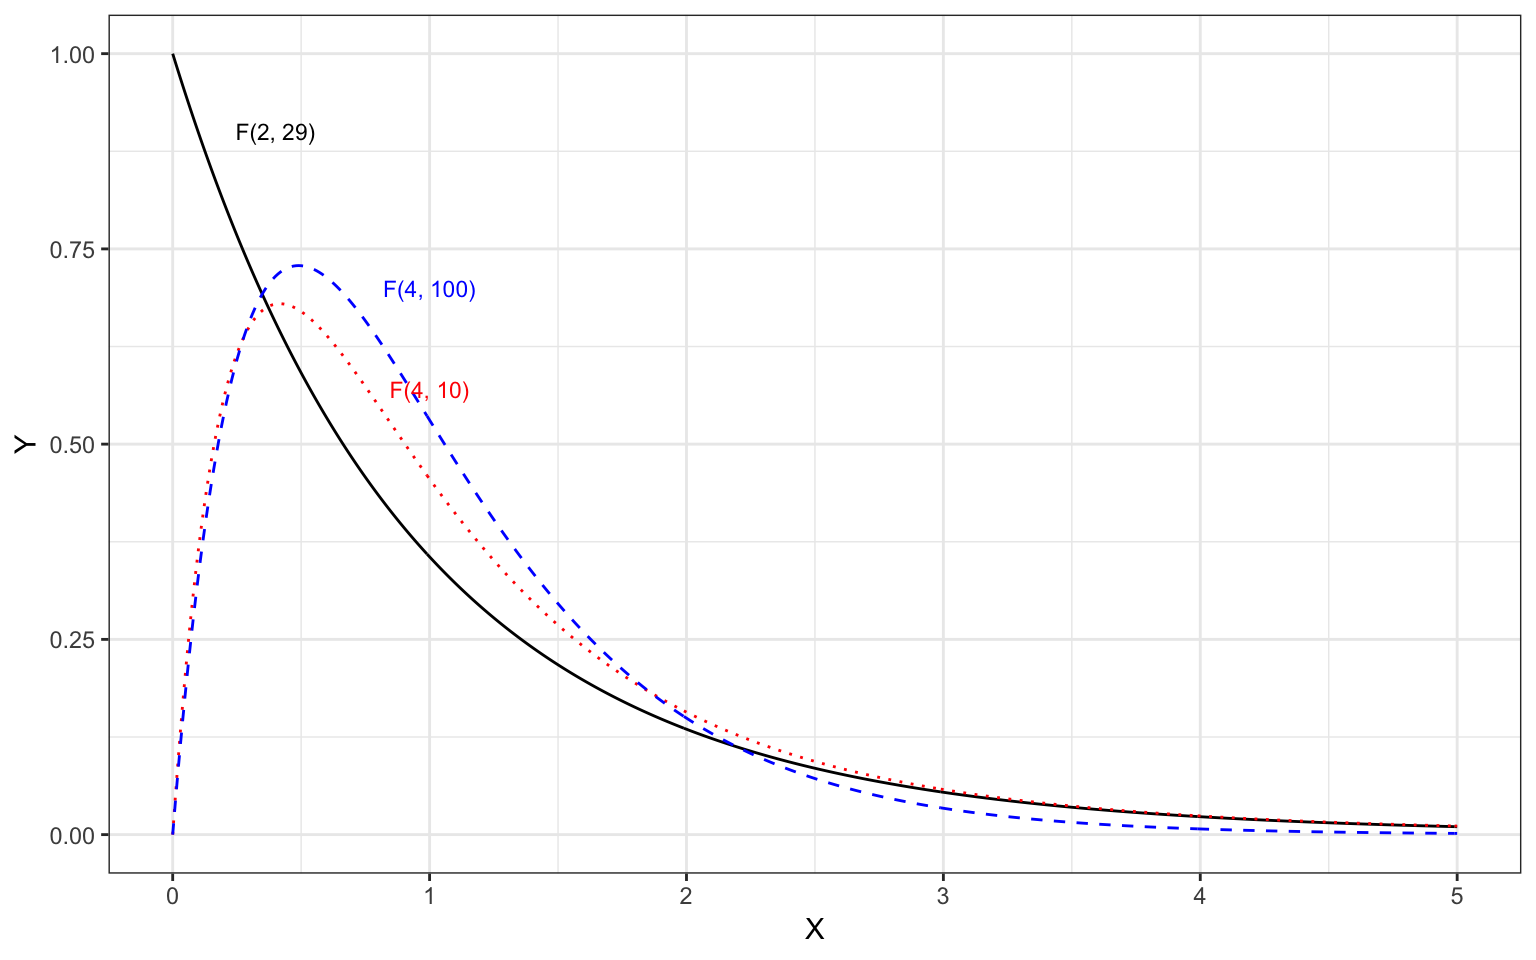
\includegraphics[width=0.8\linewidth]{epsy-8252-notes_files/figure-latex/unnamed-chunk-112-1} 

}

\caption{Plot of several F-distributions with differing degrees of freedom. The F(2,29)-distribution is shown as a solid, black line.}\label{fig:unnamed-chunk-112}
\end{figure}

The \(F\)-distribution, like the \(t\)-distribution is a family of distributions. They are positively skewed and generally have a lower-limit of 0. Because of this, when we use the \(F\)-distribution to compute a \(p\)-value, we only compute the cumulative density GREATER THAN OR EQUAL TO the value of the standardized test statistic.

\hypertarget{computing-f-from-the-anova-partitioning}{%
\subsubsection{Computing F from the ANOVA Partitioning}\label{computing-f-from-the-anova-partitioning}}

We can also compute the model-level \(F\)-statistic using the partitioning of variation from the ANOVA table.

\begin{Shaded}
\begin{Highlighting}[]
\KeywordTok{anova}\NormalTok{(lm}\FloatTok{.1}\NormalTok{)}
\end{Highlighting}
\end{Shaded}

\begin{verbatim}
Analysis of Variance Table

Response: income
          Df     Sum Sq    Mean Sq F value       Pr(>F)    
education  1 4147330492 4147330492    70.9 0.0000000028 ***
seniority  1  722883649  722883649    12.4       0.0015 ** 
Residuals 29 1695313285   58459079                         
---
Signif. codes:  0 '***' 0.001 '**' 0.01 '*' 0.05 '.' 0.1 ' ' 1
\end{verbatim}

The \(F\)-statistic is a ratio of the mean square for the model and the mean square for the error. To compute a mean square we use the general computation

\[
\mathrm{MS} = \frac{\mathrm{SS}}{\mathrm{df}}
\]

The model includes both the education and seniority predictor, so we combine the SS and df. The MS model is:

\[
\begin{split}
\mathrm{MS}_{\mathrm{Model}} &= \frac{\mathrm{SS}_{\mathrm{Model}}}{\mathrm{df}_{\mathrm{Model}}} \\
&= \frac{4147330492 + 722883649}{1 + 1} \\
&= \frac{4870214141}{2} \\
&= 2435107070
\end{split}
\]

The MS error is:

\[
\begin{split}
\mathrm{MS}_{\mathrm{Error}} &= \frac{\mathrm{SS}_{\mathrm{Error}}}{\mathrm{df}_{\mathrm{Error}}} \\
&= \frac{1695313285 }{29} \\
&= 58459079
\end{split}
\]

Then, we compute the \(F\)-statistic by computing the ratio of these two mean squares.

\[
\begin{split}
F &= \frac{\mathrm{MS}_{\mathrm{Model}}}{\mathrm{MS}_{\mathrm{Error}}} \\
&= \frac{2435107070}{58459079} \\
&= 41.7
\end{split}
\]

This is the observed \(F\)-statistic for the model. Note that this is an identical computation (although reframed) as the initial computation for \(F\).

\$\$
\textbackslash{}begin\{split\}
F \&= \frac{R^2}{1-R^2} \times \frac{\mathrm{df}_{\mathrm{Error}}}{\mathrm{df}_{\mathrm{Model}}} \textbackslash{}{[}1em{]}
\&= \frac{\frac{\mathrm{SS}_{\mathrm{Model}}}{\mathrm{SS}_{\mathrm{Total}}}}{\frac{\mathrm{SS}_{\mathrm{Error}}}{\mathrm{SS}_{\mathrm{Total}}}} \times \frac{\mathrm{df}_{\mathrm{Error}}}{\mathrm{df}_{\mathrm{Model}}} \textbackslash{}{[}1em{]}
\&= \frac{\mathrm{SS}_{\mathrm{Model}}}{\mathrm{SS}_{\mathrm{Error}}} \times \frac{\mathrm{df}_{\mathrm{Error}}}{\mathrm{df}_{\mathrm{Model}}} \textbackslash{}{[}1em{]}
\&= \frac{\mathrm{SS}_{\mathrm{Model}}}{\mathrm{df}_{\mathrm{Model}}} \times \frac{\mathrm{df}_{\mathrm{Error}}}{\mathrm{SS}_{\mathrm{Error}}} \textbackslash{}{[}1em{]}

\&= \mathrm{MS}\_\{\mathrm{Model}\} \times \frac{1}{\mathrm{MS}_{\mathrm{Error}}}\textbackslash{}{[}1em{]}
\&= \frac{\mathrm{MS}_{\mathrm{Model}}}{\mathrm{MS}_{\mathrm{Error}}}
\textbackslash{}end\{split\}
\$\$

To test the null hypothesis, \(H_0:\rho^2=0\), we evaluate this observed \(F\)-statistic in an \(F\)-distribution with the 2 and 29 degrees of freedom.

\begin{figure}

{\centering 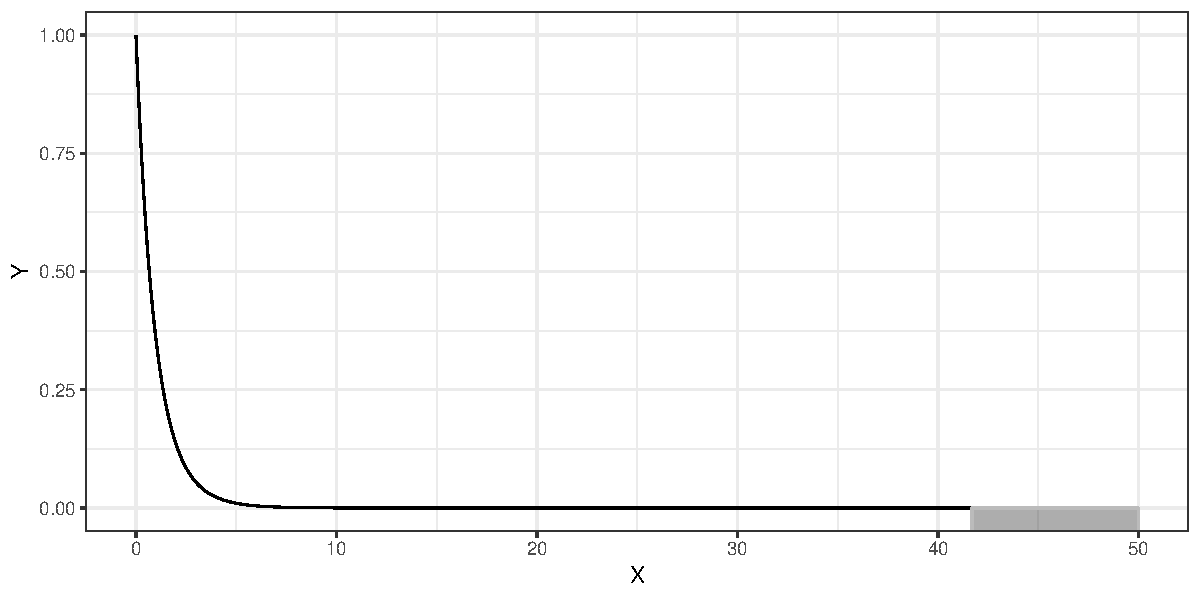
\includegraphics[width=0.8\linewidth]{epsy-8252-notes_files/figure-latex/unnamed-chunk-114-1} 

}

\caption{Plot of the probability density function (PDF) for the F-distribution with 2 and 29 degrees of freedom. The cumulative density representing the p-value for a two-tailed test evaluating whether rho-squared=0 using an observed F-statistic of 41.7 is also displayed.}\label{fig:unnamed-chunk-114}
\end{figure}

The computation using the cumulative density function, \texttt{pf()}, to obtain the \(p\)-value is:

\begin{Shaded}
\begin{Highlighting}[]
\DecValTok{1} \OperatorTok{-}\StringTok{ }\KeywordTok{pf}\NormalTok{(}\FloatTok{41.7}\NormalTok{, }\DataTypeTok{df1 =} \DecValTok{2}\NormalTok{, }\DataTypeTok{df2 =} \DecValTok{29}\NormalTok{)}
\end{Highlighting}
\end{Shaded}

\begin{verbatim}
[1] 0.000000002942
\end{verbatim}

\hypertarget{mean-squares-are-variance-estimates}{%
\section{Mean Squares are Variance Estimates}\label{mean-squares-are-variance-estimates}}

Mean squares are estimates of the variance. Consider the computational formula for the sample variance,

\[
\hat{\sigma}^2 = \frac{\sum(Y - \bar{Y})^2}{n-1}
\]

This is the total sum of squares divided by the total \emph{df}. When we compute an \(F\)-statistic, we are finding the ratio of two different variance estimates---one based on the model (explained variance) and one based on the error (unexplained variance). Under the null hypothesis that \(\rho^2 = 0\), we are assuming that all the variance is unexplained. In that case, our \(F\)-statistic would be close to zero. When the model explains a significant amount of variation, the numerator gets larger relative to the denominator and the \(F\)-value is larger.

The mean squared error (from the \texttt{anova()} output) plays a special role in regression analysis. It is the variance estimate for the conditional distributions of the residuals in our visual depiction of the distributional assumptions of the residuals underlying linear regression.

\begin{figure}

{\centering 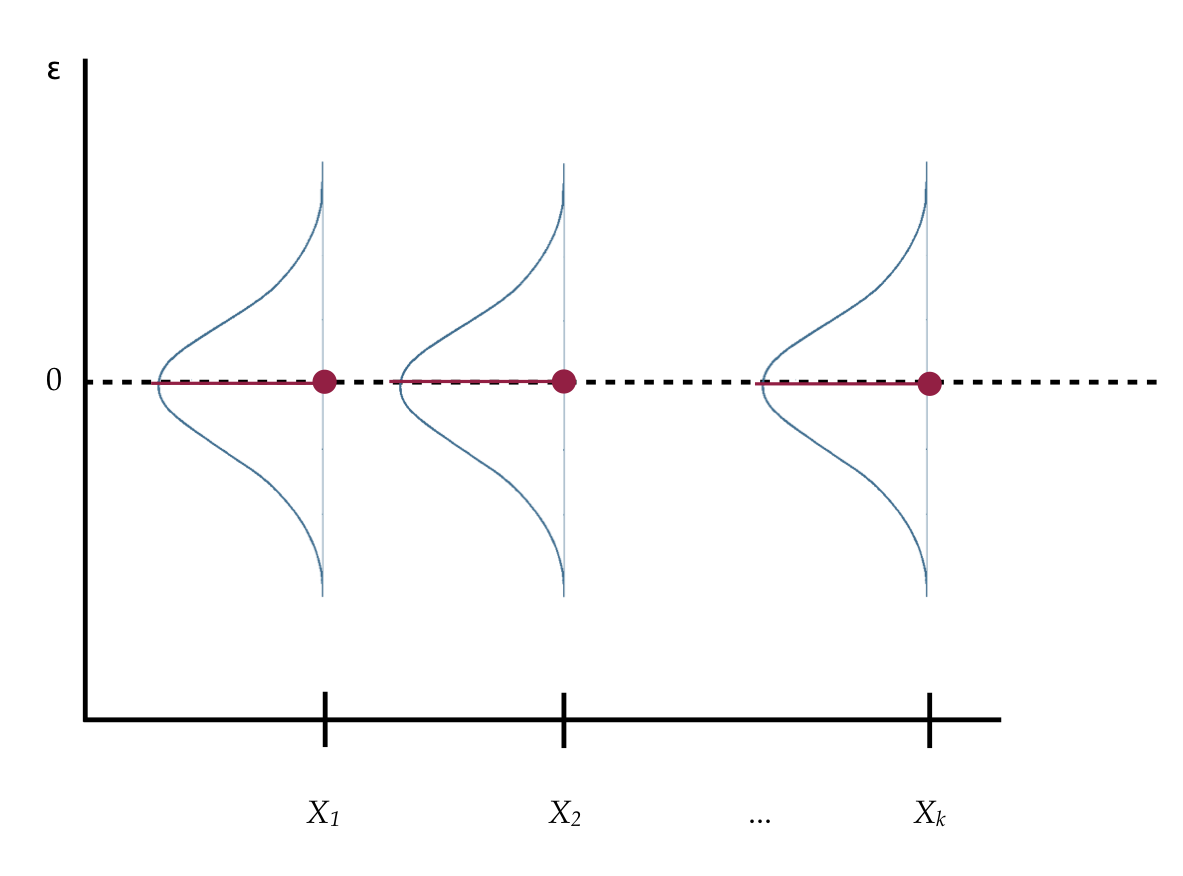
\includegraphics[width=0.7\linewidth]{images/regression-assumptions-residuals} 

}

\caption{Visual depiction of the distributional assumptions of the residuals underlying linear regression.}\label{fig:unnamed-chunk-116}
\end{figure}

Recall that we made implicit assumptions about the conditional distributions of the residuals, namely that they were identically and normally distributed with a mean of zero and some variance. Based on the estimate of the mean squared error, the variance of each of these distributions is 58,459,079.

While the variance is a mathematical convenience, the standard deviation is a better descriptor of the variation in these distributions. The standard deviation is 7646.

\begin{Shaded}
\begin{Highlighting}[]
\KeywordTok{sqrt}\NormalTok{(}\DecValTok{58459079}\NormalTok{)}
\end{Highlighting}
\end{Shaded}

\begin{verbatim}
[1] 7646
\end{verbatim}

We can also obtain this value from the model-level regression output. Here it is typically referred to as the \emph{Root Mean Squared Error} (RMSE). In the \texttt{glance()} output this value is in the \texttt{sigma} column.

\begin{Shaded}
\begin{Highlighting}[]
\KeywordTok{glance}\NormalTok{(lm}\FloatTok{.1}\NormalTok{)}
\end{Highlighting}
\end{Shaded}

\begin{verbatim}
# A tibble: 1 x 11
  r.squared adj.r.squared sigma statistic p.value    df logLik   AIC   BIC
      <dbl>         <dbl> <dbl>     <dbl>   <dbl> <int>  <dbl> <dbl> <dbl>
1     0.742         0.724 7646.      41.7 2.98e-9     3  -330.  668.  674.
# ... with 2 more variables: deviance <dbl>, df.residual <int>
\end{verbatim}

Why is this value important? It gives the expected variation in the distribution. For example, since all of the conditional distributions of the residuals are normally distributed, we would expect that 95\% of the residuals would fall between \(\pm2\) standard errors from 0; or, in this case, between \(-15292\) and 15292. Observations with residuals that are more extreme may be regression outliers.

\hypertarget{maximum-likelihood-estimation}{%
\chapter{Maximum Likelihood Estimation}\label{maximum-likelihood-estimation}}

In this set of notes, you will learn about the method of maximum likelihood to estimate model parameters.

\begin{center}\rule{0.5\linewidth}{\linethickness}\end{center}

\hypertarget{preparation-4}{%
\subsection*{Preparation}\label{preparation-4}}
\addcontentsline{toc}{subsection}{Preparation}

Before class you will need read the following:

\begin{itemize}
\tightlist
\item
  Section 3.1.2: Random Variables in Fox {[}Required Textbook{]}
\item
  Myung, J. (2003). \href{http://times.cs.uiuc.edu/course/410/note/mle.pdf}{Tutorial on maximum likelihood estimation}. \emph{Journal of Mathematical Psychology, 47}, 90--100.
\end{itemize}

\begin{center}\rule{0.5\linewidth}{\linethickness}\end{center}

\hypertarget{dataset-and-research-question-3}{%
\section{Dataset and Research Question}\label{dataset-and-research-question-3}}

In this set of notes, we will not be using a specific dataset.

\begin{Shaded}
\begin{Highlighting}[]
\CommentTok{# Load libraries}
\KeywordTok{library}\NormalTok{(broom)}
\KeywordTok{library}\NormalTok{(dplyr)}
\KeywordTok{library}\NormalTok{(ggplot2)}
\KeywordTok{library}\NormalTok{(readr)}
\KeywordTok{library}\NormalTok{(sm)}
\KeywordTok{library}\NormalTok{(tidyr)}
\end{Highlighting}
\end{Shaded}

\hypertarget{joint-probability-density}{%
\section{Joint Probability Density}\label{joint-probability-density}}

In the previous set of notes, we discussed the probability density of an observation \(X_i\). Now we will extend this idea to the probability density of a set of observations, say \(x_1\), \(x_2\), \ldots AND \(x_k\). The probability density of a set of observations is referred to as the \emph{joint probability density}, or simply \emph{joint density}.

If we can make an assumption about INDEPENDENCE, then the joint probability density would be the product of the individual densities:

\[
p(x_1, x_2, x_3, \ldots, x_K) = p(x_1) \times p(x_2) \times p(x_3) \times \ldots \times p(x_k)
\]

Say we had three independent observations from our \(\sim\mathcal{N}(50,10)\) distribution, namely \(x =\{60, 65, 67\}\). Then the joint density would be,

\begin{Shaded}
\begin{Highlighting}[]
\KeywordTok{dnorm}\NormalTok{(}\DataTypeTok{x =} \DecValTok{60}\NormalTok{, }\DataTypeTok{mean =} \DecValTok{50}\NormalTok{, }\DataTypeTok{sd =} \DecValTok{10}\NormalTok{) }\OperatorTok{*}\StringTok{ }\KeywordTok{dnorm}\NormalTok{(}\DataTypeTok{x =} \DecValTok{65}\NormalTok{, }\DataTypeTok{mean =} \DecValTok{50}\NormalTok{, }\DataTypeTok{sd =} \DecValTok{10}\NormalTok{) }\OperatorTok{*}\StringTok{ }\KeywordTok{dnorm}\NormalTok{(}\DataTypeTok{x =} \DecValTok{67}\NormalTok{, }\DataTypeTok{mean =} \DecValTok{50}\NormalTok{, }\DataTypeTok{sd =} \DecValTok{10}\NormalTok{)}
\end{Highlighting}
\end{Shaded}

\begin{verbatim}
[1] 0.000002947
\end{verbatim}

We could also shortcut this computation,

\begin{Shaded}
\begin{Highlighting}[]
\KeywordTok{prod}\NormalTok{(}\KeywordTok{dnorm}\NormalTok{(}\DataTypeTok{x =} \KeywordTok{c}\NormalTok{(}\DecValTok{60}\NormalTok{, }\DecValTok{65}\NormalTok{, }\DecValTok{67}\NormalTok{), }\DataTypeTok{mean =} \DecValTok{50}\NormalTok{, }\DataTypeTok{sd =} \DecValTok{10}\NormalTok{))}
\end{Highlighting}
\end{Shaded}

\begin{verbatim}
[1] 0.000002947
\end{verbatim}

This value is the joint probability density. The joint probability density indicates the probability of observing the data (\(x =\{60, 65, 67\}\)) GIVEN (1) they are drawn from a normal distribution and (2) the normal distribution has a mean of 50 and a standard deviation of 10. In other words:

\begin{quote}
The joint probability density is the probability of the data given the distribution and parameters.
\end{quote}

Symbolically,

\[
\mathrm{Joint~Density} = P(\mathrm{Data} \mid \mathrm{Distribution~and~Parameters})
\]

\hypertarget{likelihood}{%
\section{Likelihood}\label{likelihood}}

Likelihood is the probability of a particular set of parameters GIVEN (1) the data, and (2) the data are from a particular distribution (e.g., normal). Symbolically,

\[
\mathrm{Likelihood} = P(\mathrm{Parameters} \mid \mathrm{Distribution~and~Data})
\]

Likelihood takes the data as given and computes the probability of a set of parameters. Symbolically we denote likelihood with a scripted letter ``L'' (\(\mathcal{L}\)). For example, we might ask the question, given the observed data \(x = \{30, 20, 24, 27\}\) come from a normal distribution, what is the likelihood (probability) that the mean is 20 and the standard deviation is 4? We might denote this as,

\[
\mathcal{L}(\mu = 20, \sigma =4 \mid x)
\]

Note that although we need to specify the distribution (e.g., normal), this is typically not included in the symbolic notation; instead it is typically included in the assumptions.

The likelihood allows us to answer probability questions about a set of parameters. For example, what is the likelihood (probability) that the data (\(x = \{30, 20, 24, 27\}\)) were generated from a normal distribution with a mean of 20 and standard deviation of 4? To compute the likelihood we compute the joint probability density of the data under that particular set of parameters.

\begin{Shaded}
\begin{Highlighting}[]
\KeywordTok{prod}\NormalTok{(}\KeywordTok{dnorm}\NormalTok{(}\DataTypeTok{x =} \KeywordTok{c}\NormalTok{(}\DecValTok{30}\NormalTok{, }\DecValTok{20}\NormalTok{, }\DecValTok{24}\NormalTok{, }\DecValTok{27}\NormalTok{), }\DataTypeTok{mean =} \DecValTok{20}\NormalTok{, }\DataTypeTok{sd =} \DecValTok{4}\NormalTok{))}
\end{Highlighting}
\end{Shaded}

\begin{verbatim}
[1] 0.0000005703
\end{verbatim}

What is the likelihood (probability) that the data (\(x = \{30, 20, 24, 27\}\)) were generated from a normal distribution with a mean of 25 and standard deviation of 4?

\begin{Shaded}
\begin{Highlighting}[]
\KeywordTok{prod}\NormalTok{(}\KeywordTok{dnorm}\NormalTok{(}\DataTypeTok{x =} \KeywordTok{c}\NormalTok{(}\DecValTok{30}\NormalTok{, }\DecValTok{20}\NormalTok{, }\DecValTok{24}\NormalTok{, }\DecValTok{27}\NormalTok{), }\DataTypeTok{mean =} \DecValTok{25}\NormalTok{, }\DataTypeTok{sd =} \DecValTok{4}\NormalTok{))}
\end{Highlighting}
\end{Shaded}

\begin{verbatim}
[1] 0.00001774
\end{verbatim}

It is important to note that although we use the joint probability under a set of parameters to compute the likelihood of those parameters, theoretically joint density and likelihood are very different. Likelihood refers to the probability of the parameters and joint probability density refers to the probability of the data.

\hypertarget{maximum-likelihood}{%
\section{Maximum Likelihood}\label{maximum-likelihood}}

Which set of parameters,\(\mathcal{N}(20,4)\) or \(\mathcal{N}(25,4)\), was \emph{more likely} to generate the given data? Since the second set of parameters produced a higher likelihood, the data was more likely to have been generated from the \(\mathcal{N}(25,4)\) distribution that the \(\mathcal{N}(20,4)\) distribution.

So now we come to the crux of Maximum Likelihood Estimation (MLE). The goal of MLE is to find a set of parameters that MAXIMIZES the likelihood given the data and a distribution. For example, given the observed data \(x = \{30, 20, 24, 27\}\) were generated from a normal distribution, what are the values for the parameters of this distribution (mean and standard deviation) that produce the HIGHEST (or maximum) value of the likelihood?

Below, we will examine a couple different methods for determining the parameter values that produce the maximum value of the likelihood.

\hypertarget{method-1-grid-search}{%
\subsection{Method 1: Grid Search}\label{method-1-grid-search}}

One method for finding the parameters (in our example, the mean and standard deviation) that produce the maximum likelihood, is to substitute several parameter values in the \texttt{dnorm()} function, compute the likelihood for each set of parameters, and determine which set produces the highest (maximum) likelihood.

In computer science, this method for finding the MLE is referred to as a \emph{grid search}. Below is some syntax to carry out a grid search. The syntax creates several sets of parameter values (called the search space), computes the likelihood for each combination of parameter values, and then arranges the likelihoods in descending order.

\begin{Shaded}
\begin{Highlighting}[]
\KeywordTok{crossing}\NormalTok{(}
  \DataTypeTok{mu =} \KeywordTok{seq}\NormalTok{(}\DataTypeTok{from =} \DecValTok{10}\NormalTok{, }\DataTypeTok{to =} \DecValTok{30}\NormalTok{, }\DataTypeTok{by =} \FloatTok{0.1}\NormalTok{),}
  \DataTypeTok{sigma =} \KeywordTok{seq}\NormalTok{(}\DataTypeTok{from =} \DecValTok{0}\NormalTok{, }\DataTypeTok{to =} \DecValTok{10}\NormalTok{, }\DataTypeTok{by =} \FloatTok{0.1}\NormalTok{)}
\NormalTok{  ) }\OperatorTok
\StringTok{  }\KeywordTok{rowwise}\NormalTok{() }\OperatorTok
\StringTok{  }\KeywordTok{mutate}\NormalTok{(}
    \DataTypeTok{L =} \KeywordTok{prod}\NormalTok{(}\KeywordTok{dnorm}\NormalTok{(}\KeywordTok{c}\NormalTok{(}\DecValTok{30}\NormalTok{, }\DecValTok{20}\NormalTok{, }\DecValTok{24}\NormalTok{, }\DecValTok{27}\NormalTok{), }\DataTypeTok{mean =}\NormalTok{ mu, }\DataTypeTok{sd =}\NormalTok{ sigma))}
\NormalTok{    ) }\OperatorTok
\StringTok{  }\KeywordTok{arrange}\NormalTok{(}\KeywordTok{desc}\NormalTok{(L))}
\end{Highlighting}
\end{Shaded}

\begin{verbatim}
# A tibble: 20,301 x 3
      mu sigma         L
   <dbl> <dbl>     <dbl>
 1  25.2   3.7 0.0000183
 2  25.3   3.7 0.0000183
 3  25.3   3.8 0.0000182
 4  25.2   3.8 0.0000182
 5  25.4   3.7 0.0000182
 6  25.1   3.7 0.0000182
 7  25.2   3.6 0.0000182
 8  25.3   3.6 0.0000182
 9  25.1   3.8 0.0000182
10  25.4   3.8 0.0000182
# ... with 20,291 more rows
\end{verbatim}

The parameters that maximize the likelihood (in our search space) are a mean of 25.2 and a standard deviation of 3.7.

\hypertarget{log-likelihood}{%
\subsection{Log-Likelihood}\label{log-likelihood}}

The likelihood values are quite small since we are multiplying several probabilities together. We could take the natural logarithm of the likelihood to alleviate this issue. So in our example, \(\mathcal{L} = .00001829129\) and the log-likelihood would be

\begin{Shaded}
\begin{Highlighting}[]
\KeywordTok{log}\NormalTok{(.}\DecValTok{00001829129}\NormalTok{)}
\end{Highlighting}
\end{Shaded}

\begin{verbatim}
[1] -10.91
\end{verbatim}

We typically denote log-likelihood using a scripted lower-case ``l'' (\(\mathcal{l}\)). Going back to how we compute the likelihood, we assumed a set of parameters and then found the joint probability density, which assuming normality and independence is the product of the individual densities.

\[
\mathcal{L}(\mathrm{parameters} | \mathrm{data}) = p(x_1) \times p(x_2) \times \ldots \times p(x_n)
\]

If we compute the log of the likelihood instead:

\[
\mathcal{l}(\mathrm{parameters} | \mathrm{data}) =  \ln \Bigl(\mathcal{L}(\mathrm{parameters} | \mathrm{data})\Bigr) = \ln \Bigl(p(x_1) \times p(x_2) \times \ldots \times p(x_n)\Bigr)
\]

Using the rules of logarithms, the right-hand side of the equation can be manipulated to:

\[
= \ln \Bigl(p(x_1)\Bigr) + \ln \Bigl(p(x_2)\Bigr) + \ldots + \ln \Bigl(p(x_n)\Bigr)
\]

The log-likelihood is the \emph{sum of the log-transformed densities}. This means we could re-write our grid search syntax to compute the log-likelihood. Since finding the log of the densities is so useful, there is even an argument in \texttt{dnorm()} of \texttt{log=TRUE} that does this for us. Our revised grid search syntax is:

\begin{Shaded}
\begin{Highlighting}[]
\KeywordTok{crossing}\NormalTok{(}
  \DataTypeTok{mu =} \KeywordTok{seq}\NormalTok{(}\DataTypeTok{from =} \DecValTok{10}\NormalTok{, }\DataTypeTok{to =}\DecValTok{30}\NormalTok{, }\DataTypeTok{by =} \FloatTok{0.1}\NormalTok{),}
  \DataTypeTok{sigma =} \KeywordTok{seq}\NormalTok{(}\DataTypeTok{from =} \DecValTok{0}\NormalTok{, }\DataTypeTok{to =} \DecValTok{10}\NormalTok{, }\DataTypeTok{by =} \FloatTok{0.1}\NormalTok{)}
\NormalTok{  ) }\OperatorTok
\StringTok{  }\KeywordTok{rowwise}\NormalTok{() }\OperatorTok
\StringTok{  }\KeywordTok{mutate}\NormalTok{(}
    \DataTypeTok{log_L =} \KeywordTok{sum}\NormalTok{(}\KeywordTok{dnorm}\NormalTok{(}\KeywordTok{c}\NormalTok{(}\DecValTok{30}\NormalTok{, }\DecValTok{20}\NormalTok{, }\DecValTok{24}\NormalTok{, }\DecValTok{27}\NormalTok{), }\DataTypeTok{mean =}\NormalTok{ mu, }\DataTypeTok{sd =}\NormalTok{ sigma, }\DataTypeTok{log =} \OtherTok{TRUE}\NormalTok{))}
\NormalTok{    ) }\OperatorTok
\StringTok{  }\KeywordTok{arrange}\NormalTok{(}\KeywordTok{desc}\NormalTok{(log_L))}
\end{Highlighting}
\end{Shaded}

\begin{verbatim}
# A tibble: 20,301 x 3
      mu sigma log_L
   <dbl> <dbl> <dbl>
 1  25.2   3.7 -10.9
 2  25.3   3.7 -10.9
 3  25.3   3.8 -10.9
 4  25.2   3.8 -10.9
 5  25.1   3.7 -10.9
 6  25.4   3.7 -10.9
 7  25.3   3.6 -10.9
 8  25.2   3.6 -10.9
 9  25.1   3.8 -10.9
10  25.4   3.8 -10.9
# ... with 20,291 more rows
\end{verbatim}

Maximizing the log-likelihood gives the same parameter values as maximizing the likelihood. Remember that the log computation keeps the same ordination of values as the original data, so maximizing the log-likelihood is the same as maximizing the likelihood.

\hypertarget{maximum-likelihood-estimation-for-regression}{%
\section{Maximum Likelihood Estimation for Regression}\label{maximum-likelihood-estimation-for-regression}}

In model fitting, the components we care about are the residuals. Those are the things we put distributional assumptions on (e.g., normality, homogeneity of variance, independence). Our goal in regression is to estimate a set of parameters (\(\beta_0\), \(\beta_1\)) that maximize the likelihood for a given set of residuals that come from a normal distribution.

To understand this, let's use a toy example of \(n=10\) observations.

\begin{verbatim}
   x  y
1  4 53
2  0 56
3  3 37
4  4 55
5  7 50
6  0 36
7  0 22
8  3 75
9  0 37
10 2 42
\end{verbatim}

To begin, we can enter these observations into two vectors, \(x\) and \(y\).

\begin{Shaded}
\begin{Highlighting}[]
\CommentTok{# Enter data into vectors}
\NormalTok{x =}\StringTok{ }\KeywordTok{c}\NormalTok{(}\DecValTok{4}\NormalTok{, }\DecValTok{0}\NormalTok{, }\DecValTok{3}\NormalTok{, }\DecValTok{4}\NormalTok{, }\DecValTok{7}\NormalTok{, }\DecValTok{0}\NormalTok{, }\DecValTok{0}\NormalTok{, }\DecValTok{3}\NormalTok{, }\DecValTok{0}\NormalTok{, }\DecValTok{2}\NormalTok{)}
\NormalTok{y =}\StringTok{ }\KeywordTok{c}\NormalTok{(}\DecValTok{53}\NormalTok{, }\DecValTok{56}\NormalTok{, }\DecValTok{37}\NormalTok{, }\DecValTok{55}\NormalTok{, }\DecValTok{50}\NormalTok{, }\DecValTok{36}\NormalTok{, }\DecValTok{22}\NormalTok{, }\DecValTok{75}\NormalTok{, }\DecValTok{37}\NormalTok{, }\DecValTok{42}\NormalTok{)}
\end{Highlighting}
\end{Shaded}

Next, we will write a function to compute the log-likelihood (or likelihood) of the residuals given particular \texttt{b0} and \texttt{b1} estimates that will be inputted to the function.

One issue is that in using the \texttt{dnorm()} function we need to specify the mean and standard deviation. The regression assumptions help with this task. The conditional mean residual value is 0. So we will set the mean value to 0. The assumption about the standard deviation is that the conditional distributions all have the same SD, but it doesn't specify what that is. However, the SD of the errors seems like a reasonable value, so let's use that.

Below, we will write a function called \texttt{log\_likelihood()} that takes two arguments as input, \texttt{b0=} and \texttt{b1=}, and outputs the log-likelihood.

\begin{Shaded}
\begin{Highlighting}[]
\NormalTok{log_likelihood =}\StringTok{ }\ControlFlowTok{function}\NormalTok{(b0, b1)\{}
  \CommentTok{# Use the following x and y values}
\NormalTok{  x =}\StringTok{ }\KeywordTok{c}\NormalTok{(}\DecValTok{4}\NormalTok{, }\DecValTok{0}\NormalTok{, }\DecValTok{3}\NormalTok{, }\DecValTok{4}\NormalTok{, }\DecValTok{7}\NormalTok{, }\DecValTok{0}\NormalTok{, }\DecValTok{0}\NormalTok{, }\DecValTok{3}\NormalTok{, }\DecValTok{0}\NormalTok{, }\DecValTok{2}\NormalTok{)}
\NormalTok{  y =}\StringTok{ }\KeywordTok{c}\NormalTok{(}\DecValTok{53}\NormalTok{, }\DecValTok{56}\NormalTok{, }\DecValTok{37}\NormalTok{, }\DecValTok{55}\NormalTok{, }\DecValTok{50}\NormalTok{, }\DecValTok{36}\NormalTok{, }\DecValTok{22}\NormalTok{, }\DecValTok{75}\NormalTok{, }\DecValTok{37}\NormalTok{, }\DecValTok{42}\NormalTok{)}
  
  \CommentTok{# Compute the yhat and residuals based on the two input values}
\NormalTok{  yhats =}\StringTok{ }\NormalTok{b0 }\OperatorTok{+}\StringTok{ }\NormalTok{b1}\OperatorTok{*}\NormalTok{x}
\NormalTok{  errors =}\StringTok{ }\NormalTok{y }\OperatorTok{-}\StringTok{ }\NormalTok{yhats}
  
  \CommentTok{# Compute the sd of the residuals}
\NormalTok{  sigma =}\StringTok{ }\KeywordTok{sd}\NormalTok{(errors)}
  
  \CommentTok{# Compute the log-likelihood}
\NormalTok{  log_lik =}\StringTok{ }\KeywordTok{sum}\NormalTok{(}\KeywordTok{dnorm}\NormalTok{(errors, }\DataTypeTok{mean =} \DecValTok{0}\NormalTok{, }\DataTypeTok{sd =}\NormalTok{ sigma, }\DataTypeTok{log =} \OtherTok{TRUE}\NormalTok{))}
  
  \CommentTok{# Output the log-likelihood}
  \KeywordTok{return}\NormalTok{(log_lik)}
\NormalTok{\}}
\end{Highlighting}
\end{Shaded}

Now we read in our function by highlighting the whole thing and running it. Once it has been read in, we can use it just like any other function. For example to find the log-likelihood for the parameters \(\beta_0=10\) and \(\beta_1=3\) we use:

\begin{Shaded}
\begin{Highlighting}[]
\KeywordTok{log_likelihood}\NormalTok{(}\DataTypeTok{b0 =} \DecValTok{10}\NormalTok{, }\DataTypeTok{b1 =} \DecValTok{3}\NormalTok{)}
\end{Highlighting}
\end{Shaded}

\begin{verbatim}
[1] -64.29
\end{verbatim}

We can also use our function in a grid search.

\begin{Shaded}
\begin{Highlighting}[]
\KeywordTok{crossing}\NormalTok{(}
  \DataTypeTok{b0 =} \KeywordTok{seq}\NormalTok{(}\DataTypeTok{from =} \DecValTok{30}\NormalTok{, }\DataTypeTok{to =} \DecValTok{50}\NormalTok{, }\DataTypeTok{by =} \FloatTok{0.1}\NormalTok{),}
  \DataTypeTok{b1 =} \KeywordTok{seq}\NormalTok{(}\DataTypeTok{from =} \DecValTok{-5}\NormalTok{, }\DataTypeTok{to =} \DecValTok{5}\NormalTok{, }\DataTypeTok{by =} \FloatTok{0.1}\NormalTok{)}
\NormalTok{) }\OperatorTok
\StringTok{  }\KeywordTok{rowwise}\NormalTok{() }\OperatorTok
\StringTok{  }\KeywordTok{mutate}\NormalTok{(}
    \DataTypeTok{log_L =} \KeywordTok{log_likelihood}\NormalTok{(}\DataTypeTok{b0 =}\NormalTok{ b0, }\DataTypeTok{b1 =}\NormalTok{ b1)}
\NormalTok{    ) }\OperatorTok
\StringTok{  }\KeywordTok{arrange}\NormalTok{(}\KeywordTok{desc}\NormalTok{(log_L))}
\end{Highlighting}
\end{Shaded}

\begin{verbatim}
# A tibble: 20,301 x 3
      b0    b1 log_L
   <dbl> <dbl> <dbl>
 1  40.1   2.7 -39.5
 2  40     2.7 -39.5
 3  40.2   2.7 -39.5
 4  39.9   2.8 -39.5
 5  39.8   2.8 -39.5
 6  40     2.8 -39.5
 7  39.9   2.7 -39.5
 8  39.7   2.8 -39.5
 9  40.3   2.7 -39.5
10  40.1   2.8 -39.5
# ... with 20,291 more rows
\end{verbatim}

Here the parameter values that maximize the likelihood are \(\beta_0 = 40.1\) and \(\beta_1=2.7\). We can also compute what the standard deviation for the residual distributions was using the estimated parameter values. Remember, this value is an estimate of the RMSE.

\begin{Shaded}
\begin{Highlighting}[]
\NormalTok{errors =}\StringTok{ }\NormalTok{y }\OperatorTok{-}\StringTok{ }\FloatTok{40.1} \OperatorTok{-}\StringTok{ }\FloatTok{2.7}\OperatorTok{*}\NormalTok{x}
\KeywordTok{sd}\NormalTok{(errors)}
\end{Highlighting}
\end{Shaded}

\begin{verbatim}
[1] 13.19
\end{verbatim}

In practice, there are a couple subtle differences, namely that the estimate for the SD value we use in \texttt{dnorm()} is slightly different. This generally does not have an effect on the coefficient estimates, but does impact the estimate of the RMSE. We will talk more about this when we talk about \emph{Restricted Maximum Likelihood Estimation} (REML).

\hypertarget{large-search-spaces}{%
\subsection{Large Search Spaces}\label{large-search-spaces}}

So far, we have been using a very finite search space that has been defined for us. For example, we limited the search space to 20,301 combinations of \(\beta_0\) and \(\beta_1\).

\begin{Shaded}
\begin{Highlighting}[]
\KeywordTok{nrow}\NormalTok{(}
  \KeywordTok{crossing}\NormalTok{(}
    \DataTypeTok{b0 =} \KeywordTok{seq}\NormalTok{(}\DataTypeTok{from =} \DecValTok{30}\NormalTok{, }\DataTypeTok{to =} \DecValTok{50}\NormalTok{, }\DataTypeTok{by =} \FloatTok{0.1}\NormalTok{),}
    \DataTypeTok{b1 =} \KeywordTok{seq}\NormalTok{(}\DataTypeTok{from =} \DecValTok{-5}\NormalTok{, }\DataTypeTok{to =} \DecValTok{5}\NormalTok{, }\DataTypeTok{by =} \FloatTok{0.1}\NormalTok{)}
\NormalTok{  )}
\NormalTok{)}
\end{Highlighting}
\end{Shaded}

\begin{verbatim}
[1] 20301
\end{verbatim}

This allowed us to find the coefficient estimates to the nearest tenth. If we instead needed to find the estimates to the nearest hundredth, we would need to expand the number of combinations:

\begin{Shaded}
\begin{Highlighting}[]
\KeywordTok{nrow}\NormalTok{(}
  \KeywordTok{crossing}\NormalTok{(}
    \DataTypeTok{b0 =} \KeywordTok{seq}\NormalTok{(}\DataTypeTok{from =} \DecValTok{30}\NormalTok{, }\DataTypeTok{to =} \DecValTok{50}\NormalTok{, }\DataTypeTok{by =} \FloatTok{0.01}\NormalTok{),}
    \DataTypeTok{b1 =} \KeywordTok{seq}\NormalTok{(}\DataTypeTok{from =} \DecValTok{-5}\NormalTok{, }\DataTypeTok{to =} \DecValTok{5}\NormalTok{, }\DataTypeTok{by =} \FloatTok{0.01}\NormalTok{)}
\NormalTok{  )}
\NormalTok{)}
\end{Highlighting}
\end{Shaded}

\begin{verbatim}
[1] 2003001
\end{verbatim}

This leads to a search space of 2,003,001 parameter combinations. If we need them to the nearest thousandth, the search space is 200,030,001 combinations.

Furthermore, in practice you would not have any idea which values of \(\beta_0\) and \(\beta_1\) to limit the search space to. Essentially you would need to search an infinite number of values unless you could limit the search space in some way. For many common methods (e.g., linear regression) finding the ML estimates is mathematically pretty easy (if we know calculus; see the section \protect\hyperlink{way-too-much-math}{Way, Way, Way too Much Mathematics}). For more complex methods (e.g., mixed-effect models) there is not a mathematical solution. Instead, mathematics is used to help limit the search space and then a grid search is used to hone in on the estimates.

\hypertarget{ml-estimation-in-regression-using-r}{%
\section{ML Estimation in Regression Using R}\label{ml-estimation-in-regression-using-r}}

Recall that the \texttt{lm()} function uses Ordinary Least Squares (OLS) estimation---it finds the coefficient estimates and RMSE that minimize the sum of squared residuals.

\begin{Shaded}
\begin{Highlighting}[]
\NormalTok{lm}\FloatTok{.1}\NormalTok{ =}\StringTok{ }\KeywordTok{lm}\NormalTok{(y }\OperatorTok{~}\StringTok{ }\DecValTok{1} \OperatorTok{+}\StringTok{ }\NormalTok{x)}

\CommentTok{# Get coefficient estimates}
\KeywordTok{tidy}\NormalTok{(lm}\FloatTok{.1}\NormalTok{)}
\end{Highlighting}
\end{Shaded}

\begin{verbatim}
# A tibble: 2 x 5
  term        estimate std.error statistic  p.value
  <chr>          <dbl>     <dbl>     <dbl>    <dbl>
1 (Intercept)    40.0       6.34      6.31 0.000231
2 x               2.74      1.98      1.38 0.203   
\end{verbatim}

\begin{Shaded}
\begin{Highlighting}[]
\CommentTok{# Get estimate for RMSE}
\KeywordTok{glance}\NormalTok{(lm}\FloatTok{.1}\NormalTok{)}
\end{Highlighting}
\end{Shaded}

\begin{verbatim}
# A tibble: 1 x 11
  r.squared adj.r.squared sigma statistic p.value    df logLik   AIC   BIC
      <dbl>         <dbl> <dbl>     <dbl>   <dbl> <int>  <dbl> <dbl> <dbl>
1     0.193        0.0926  14.0      1.92   0.203     2  -39.5  84.9  85.8
# ... with 2 more variables: deviance <dbl>, df.residual <int>
\end{verbatim}

Under OLS estimation:

\begin{itemize}
\tightlist
\item
  \(\hat\beta_0 = 40.01\)
\item
  \(\hat\beta_1 = 2.74\)
\item
  \(\hat\sigma_\epsilon = 13.99\)
\end{itemize}

To compute ML estimates of the coefficients we will use the \texttt{mle2()} function from the \textbf{bbmle} package. To use the \texttt{mle2()} function, we need to provide a user-written function that returns the \emph{negative log-likelihood} given a set of parameter inputs.

For simple regression, recall that we need to estimate three parameters: \(\beta_0\), \(\beta_1\), and \(\sigma_{\epsilon}\) (RMSE). Below we have a function that inputs values for each of the three parameters, uses the inputted coefficient values to compute the residuals given the data, and returns the negative log-likelihood value assuming normality, independence, and homoscedasticity.

\begin{Shaded}
\begin{Highlighting}[]
\NormalTok{regress.ll =}\StringTok{ }\ControlFlowTok{function}\NormalTok{(b0, b1, rmse) \{ }
  \CommentTok{# Use the following x and y values}
\NormalTok{  x =}\StringTok{ }\KeywordTok{c}\NormalTok{(}\DecValTok{4}\NormalTok{, }\DecValTok{0}\NormalTok{, }\DecValTok{3}\NormalTok{, }\DecValTok{4}\NormalTok{, }\DecValTok{7}\NormalTok{, }\DecValTok{0}\NormalTok{, }\DecValTok{0}\NormalTok{, }\DecValTok{3}\NormalTok{, }\DecValTok{0}\NormalTok{, }\DecValTok{2}\NormalTok{)}
\NormalTok{  y =}\StringTok{ }\KeywordTok{c}\NormalTok{(}\DecValTok{53}\NormalTok{, }\DecValTok{56}\NormalTok{, }\DecValTok{37}\NormalTok{, }\DecValTok{55}\NormalTok{, }\DecValTok{50}\NormalTok{, }\DecValTok{36}\NormalTok{, }\DecValTok{22}\NormalTok{, }\DecValTok{75}\NormalTok{, }\DecValTok{37}\NormalTok{, }\DecValTok{42}\NormalTok{)}
  
  \CommentTok{# Compute yhats and residuals}
\NormalTok{  yhats =}\StringTok{ }\NormalTok{b0 }\OperatorTok{+}\StringTok{ }\NormalTok{b1 }\OperatorTok{*}\StringTok{ }\NormalTok{x}
\NormalTok{  errors =}\StringTok{ }\NormalTok{y }\OperatorTok{-}\StringTok{ }\NormalTok{yhats}
  
  \CommentTok{# Compute the negative log-likelihood}
\NormalTok{  neg_log_L =}\StringTok{ }\OperatorTok{-}\KeywordTok{sum}\NormalTok{(}\KeywordTok{dnorm}\NormalTok{(errors, }\DataTypeTok{mean =} \DecValTok{0}\NormalTok{, }\DataTypeTok{sd =}\NormalTok{ rmse, }\DataTypeTok{log =} \OtherTok{TRUE}\NormalTok{))}
  \KeywordTok{return}\NormalTok{(neg_log_L)}
\NormalTok{\} }
\end{Highlighting}
\end{Shaded}

Now we can implement the \texttt{mle2()} function. This function requires the argument, \texttt{minuslogl=}, which takes the user written function returning the negative log-likelihood. It also requires a list of starting values for the input parameters in the user-written function. (Here we give values close to the OLS estimates as starting values.)

\begin{Shaded}
\begin{Highlighting}[]
\CommentTok{# Fit model using ML}
\KeywordTok{library}\NormalTok{(bbmle)}
\NormalTok{mle.results =}\StringTok{ }\KeywordTok{mle2}\NormalTok{(}\DataTypeTok{minuslogl =}\NormalTok{ regress.ll, }\DataTypeTok{start =} \KeywordTok{list}\NormalTok{(}\DataTypeTok{b0 =} \FloatTok{40.0}\NormalTok{, }\DataTypeTok{b1 =} \FloatTok{2.7}\NormalTok{, }\DataTypeTok{rmse =} \FloatTok{13.98}\NormalTok{))}

\CommentTok{# View results}
\KeywordTok{summary}\NormalTok{(mle.results)}
\end{Highlighting}
\end{Shaded}

\begin{verbatim}
Maximum likelihood estimation

Call:
mle2(minuslogl = regress.ll, start = list(b0 = 40, b1 = 2.7, 
    rmse = 13.98))

Coefficients:
     Estimate Std. Error z value   Pr(z)    
b0      40.01       5.67    7.05 1.7e-12 ***
b1       2.74       1.77    1.55    0.12    
rmse    12.51       2.80    4.47 7.7e-06 ***
---
Signif. codes:  0 '***' 0.001 '**' 0.01 '*' 0.05 '.' 0.1 ' ' 1

-2 log L: 78.91 
\end{verbatim}

Under ML estimation:

\begin{itemize}
\tightlist
\item
  \(\hat\beta_0 = 40.01\)
\item
  \(\hat\beta_1 = 2.74\)
\item
  \(\hat\sigma_\epsilon = 12.51\)
\end{itemize}

Comparing the coefficient estimates (\(\hat\beta_0\) and \(\hat\beta_1\)) between the two methods of estimation, we find they are quite similar. The estimate of \(\sigma_{\epsilon}\) is different between the two estimation methods (although they are somewhat close in value).

Why do the estimates of the RMSE differ depending on the method of estimation? This is because the two methods use different formulas for computing RMSE. In OLS estimation, recall that the estimate of \(\hat\sigma_\epsilon\) was:

\[
\hat\sigma_{\epsilon}=\frac{\left(Y_i - \hat{Y}_i\right)^2}{n-2},
\]

For ML estimation, the estimate for \(\hat\sigma_\epsilon\) is:

\[
\hat\sigma_{\epsilon}=\frac{\left(Y_i - \hat{Y}_i\right)^2}{n},
\]

The smaller denominator in OLS results in a higher estimate of the variation. This, in turn, affects the size of the SE estimates for the coefficients (and thus the \(t\)- and \(p\)-values). When \(n\) is large, the differences in the estimates of \(\hat\sigma_\epsilon\) are minimal and can safely be ignored.

Lastly, we note that the value of \(-2\)(log-likelihood) is the same for both the ML and OLS estimated models. This is a useful result. It allows us to use \texttt{lm()} to estimate the coefficients from a model and then use its log-likelihood as if we had fitted the model using ML.

\hypertarget{using-r-to-directly-compute-the-likelihood-and-log-likelihood}{%
\subsection{Using R to Directly Compute the Likelihood and Log-Likelihood}\label{using-r-to-directly-compute-the-likelihood-and-log-likelihood}}

We can use R to directly compute the log-likelihood after we fit a model using the \texttt{lm()} function. To do this, we use the \texttt{logLik()} function.

\begin{Shaded}
\begin{Highlighting}[]
\NormalTok{lm}\FloatTok{.1}\NormalTok{ =}\StringTok{ }\KeywordTok{lm}\NormalTok{(y }\OperatorTok{~}\StringTok{ }\DecValTok{1} \OperatorTok{+}\StringTok{ }\NormalTok{x)}
\KeywordTok{logLik}\NormalTok{(lm}\FloatTok{.1}\NormalTok{)}
\end{Highlighting}
\end{Shaded}

\begin{verbatim}
'log Lik.' -39.45 (df=3)
\end{verbatim}

To compute the likelihood, we can use the \texttt{exp()} function to back-transform the log-likelihood to the likelihood (although generally we will work with the log-likelihood).

\begin{Shaded}
\begin{Highlighting}[]
\KeywordTok{exp}\NormalTok{(}\OperatorTok{-}\FloatTok{39.45442}\NormalTok{)}
\end{Highlighting}
\end{Shaded}

\begin{verbatim}
[1] 7.331e-18
\end{verbatim}

\hypertarget{way-too-much-math}{%
\section{Way, Way, Way too Much Mathematics}\label{way-too-much-math}}

A second, more convenient method to determine the ML estimates of the regression parameters is to use mathematics; specifically calculus. Remember, we can express the likelihood of the regression residuals mathematically as:

\[
\mathcal{L}(\beta_0, \beta_1 | \mathrm{data}) = p(\epsilon_1) \times p(\epsilon_2) \times \ldots \times p(\epsilon_n)
\]

where the probability density of each residual (assuming normality) is:

\[
p(\epsilon_i) = \frac{1}{\sigma\sqrt{2\pi}}\exp\left[-\frac{(\epsilon_i-\mu)^2}{2\sigma^2}\right]
\]

In addition to normality, which gives us the equation to compute the PDF for each residual, the regression assumptions also specify that each conditional error distribution has a mean of 0 and some variance (that is the same for all conditional error distributions). We can call it \(\sigma^2_{\epsilon}\). Substituting these values into the density function, we get,

\[
\begin{split}
p(\epsilon_i) &= \frac{1}{\sigma_{\epsilon}\sqrt{2\pi}}\exp\left[-\frac{(\epsilon_i-0)^2}{2\sigma^2_{\epsilon}}\right] \\[1em]
&= \frac{1}{\sigma_{\epsilon}\sqrt{2\pi}}\exp\left[-\frac{(\epsilon_i)^2}{2\sigma^2_{\epsilon}}\right]
\end{split}
\]

Now we use this expression for each of the \(p(\epsilon_i)\) values in the likelihood computation.

\[
\begin{split}
\mathcal{L}(\beta_0, \beta_1 | \mathrm{data}) &= p(\epsilon_1) \times p(\epsilon_2) \times \ldots \times p(\epsilon_n) \\[1em]
&= \frac{1}{\sigma_{\epsilon}\sqrt{2\pi}}\exp\left[-\frac{\epsilon_1
^2}{2\sigma^2_{\epsilon}}\right] \times \frac{1}{\sigma_{\epsilon}\sqrt{2\pi}}\exp\left[-\frac{\epsilon_2^2}{2\sigma^2_{\epsilon}}\right] \times \ldots \times \frac{1}{\sigma_{\epsilon}\sqrt{2\pi}}\exp\left[-\frac{\epsilon_n^2}{2\sigma^2_{\epsilon}}\right] 
\end{split}
\]

We can simplify this:

\[
\begin{split}
\mathcal{L}(\beta_0, \beta_1 | \mathrm{data}) &=\left[ \frac{1}{\sigma_{\epsilon}\sqrt{2\pi}} \right]^n \times \exp\left[-\frac{\epsilon_1^2}{2\sigma^2_{\epsilon}}\right] \times \exp\left[-\frac{\epsilon_2^2}{2\sigma^2_{\epsilon}}\right] \times \ldots \times \exp\left[-\frac{\epsilon_n^2}{2\sigma^2_{\epsilon}}\right] 
\end{split}
\]

Now we will take the natural logarithm of both sides of the expression:

\[
\begin{split}
\ln \Bigl(\mathcal{L}(\beta_0, \beta_1 | \mathrm{data})\Bigr) &= \ln \Biggl( \left[ \frac{1}{\sigma_{\epsilon}\sqrt{2\pi}} \right]^n \times \exp\left[-\frac{\epsilon_1^2}{2\sigma^2_{\epsilon}}\right] \times \exp\left[-\frac{\epsilon_2^2}{2\sigma^2_{\epsilon}}\right] \times \ldots \times \exp\left[-\frac{\epsilon_n^2}{2\sigma^2_{\epsilon}}\right] \Biggr) \\
\end{split}
\]

Using our rules for logarithms and re-arranging gives,

\[
\mathcal{l}(\beta_0, \beta_1 | \mathrm{data}) = -\frac{n}{2} \times \ln (2\pi\sigma^2_{\epsilon}) - \frac{1}{2\sigma^2_{\epsilon}} \times \sum \epsilon_i^2
\]

Examining this equation, we see that the log-likelihood is a function of \(n\), \(\sigma^2_{\epsilon}\) and the sum of squared residuals (SSE). The observed data define \(n\) (the sample size) and the other two components come from the residuals which are a function of the parameters and the data.

Once we have this function, calculus can be used to find the analytic maximum. Typically before we do this, we replace \(\epsilon_i\) with \(Y_i - \hat\beta_0 - \hat\beta_1(X_i)\); writing the residuals as a function of the parameters (which we are solving for) and the data.

\[
\mathcal{l}(\beta_0, \beta_1 | \mathrm{data}) = -\frac{n}{2} \times \ln (2\pi\sigma^2_{\epsilon}) - \frac{1}{2\sigma^2_{\epsilon}} \times \sum \bigg(Y_i - \hat\beta_0 - \hat\beta_1(X_i)\bigg)^2
\]

To find the analytic maximum, we compute the partial derivatives \emph{with respect to} \(\hat\beta_0\) and \(\hat\beta_1\), and set these equal to zero. This gives us a system of two equations with two unknowns (\(\hat\beta_0\) and \(\hat\beta_1\)). We can then solve this set of equations to obtain each of the parameter estimates. Then, based on these values, we can compute the estimate for the RMSE.

\hypertarget{information-criteria-for-model-selection}{%
\chapter{Information Criteria for Model Selection}\label{information-criteria-for-model-selection}}

In this set of notes, you will learn about using information criteria to select a model from a set of candidate models.

\begin{center}\rule{0.5\linewidth}{\linethickness}\end{center}

\hypertarget{preparation-5}{%
\subsection*{Preparation}\label{preparation-5}}
\addcontentsline{toc}{subsection}{Preparation}

Before class you will need read the following:

\begin{itemize}
\tightlist
\item
  Elliott, L. P., \& Brook, B. W. (2007). \href{https://academic.oup.com/bioscience/article/57/7/608/238555}{Revisiting Chamberlin: Multiple working hypotheses for the 21st century}. \emph{BioScience, 57}(7), 608--614.
\end{itemize}

\begin{center}\rule{0.5\linewidth}{\linethickness}\end{center}

\hypertarget{dataset-and-research-question-4}{%
\section{Dataset and Research Question}\label{dataset-and-research-question-4}}

In this set of notes, we will use the data in the \emph{ed-schools-2018.csv} file (see the \protect\hyperlink{ed-schools-2018}{data codebook} here). These data include institutional-level attributes for several graduate education schools/programs rated by \emph{U.S. News and World Report} in 2018.

\begin{Shaded}
\begin{Highlighting}[]
\CommentTok{# Load libraries}
\KeywordTok{library}\NormalTok{(broom)}
\KeywordTok{library}\NormalTok{(corrr)}
\KeywordTok{library}\NormalTok{(dplyr)}
\KeywordTok{library}\NormalTok{(ggplot2)}
\KeywordTok{library}\NormalTok{(readr)}
\KeywordTok{library}\NormalTok{(sm)}
\KeywordTok{library}\NormalTok{(tidyr)}

\CommentTok{# Read in data}
\NormalTok{ed =}\StringTok{ }\KeywordTok{read_csv}\NormalTok{(}\DataTypeTok{file =} \StringTok{"~/Documents/github/epsy-8252/data/ed-schools-2018.csv"}\NormalTok{)}
\KeywordTok{head}\NormalTok{(ed)}
\end{Highlighting}
\end{Shaded}

\begin{verbatim}
# A tibble: 6 x 13
   rank school score  peer expert_score gre_verbal gre_quant doc_accept
  <dbl> <chr>  <dbl> <dbl>        <dbl>      <dbl>     <dbl>      <dbl>
1     1 Harva~   100   4.4          4.6        163       159        4.5
2     2 Stanf~    99   4.6          4.8        162       160        6.1
3     3 Unive~    96   4.2          4.3        156       152       29.1
4     3 Unive~    96   4.1          4.5        163       157        5  
5     3 Unive~    96   4.3          4.5        155       153       26.1
6     6 Johns~    95   4.1          4.1        164       162       27.4
# ... with 5 more variables: phd_student_faculty_ratio <dbl>,
#   phd_granted_per_faculty <dbl>, funded_research <dbl>,
#   funded_research_per_faculty <dbl>, enroll <dbl>
\end{verbatim}

Using these data, we will examine the factors our academic peers use to rate graduate programs. To gather the peer assessment data, \emph{U.S. News} asked deans, program directors and senior faculty to judge the academic quality of programs in their field on a scale of 1 (marginal) to 5 (outstanding). Based on the substantive literature we have three \textbf{scientific working hypotheses} about how programs are rated:

\begin{itemize}
\tightlist
\item
  \textbf{H1:} Student-related factors drive the perceived academic quality of graduate programs in education.
\item
  \textbf{H2:} Faculty-related factors drive the perceived academic quality of graduate programs in education.
\item
  \textbf{H3:} Institution-related factors drive the perceived academic quality of graduate programs in education.
\end{itemize}

We need to translate these working hypotheses into statistical models that we can then fit to a set of data. The models are only proxies for the working hypotheses. However, that being said, the validity of using the models as proxies is dependent on whether we have measured well, whether the translation makes substantive sense given the literature base, etc. Here is how we are measuring the different attributes:

\begin{itemize}
\tightlist
\item
  The student-related factors we will use are GRE scores.
\item
  The faculty-related factors we will use are funded research (per faculty member) and the number of Ph.D.~graduates (per faculty member).
\item
  The institution-related factors we will use are the acceptance rate of Ph.D.~students, the Ph.D.~student-to-faculty ratio, and the size of the program.
\end{itemize}

\hypertarget{model-building}{%
\section{Model-Building}\label{model-building}}

Before we begin the exploratory analysis associated with model-building, it is worth noting that there are missing data in the dataset.

\begin{Shaded}
\begin{Highlighting}[]
\KeywordTok{summary}\NormalTok{(ed)}
\end{Highlighting}
\end{Shaded}

\begin{verbatim}
      rank          school              score            peer     
 Min.   :  1.0   Length:129         Min.   : 38.0   Min.   :2.50  
 1st Qu.: 32.0   Class :character   1st Qu.: 42.0   1st Qu.:2.90  
 Median : 62.0   Mode  :character   Median : 51.0   Median :3.20  
 Mean   : 63.2                      Mean   : 55.3   Mean   :3.29  
 3rd Qu.: 93.0                      3rd Qu.: 63.0   3rd Qu.:3.60  
  expert_score    gre_verbal    gre_quant     doc_accept   
 Min.   :2.40   Min.   :148   Min.   :142   Min.   :  4.5  
 1st Qu.:3.30   1st Qu.:152   1st Qu.:148   1st Qu.: 25.8  
 Median :3.60   Median :154   Median :150   Median : 39.8  
 Mean   :3.64   Mean   :155   Mean   :151   Mean   : 41.4  
 3rd Qu.:4.00   3rd Qu.:156   3rd Qu.:153   3rd Qu.: 54.1  
 phd_student_faculty_ratio phd_granted_per_faculty funded_research
 Min.   : 0.00             Min.   :0.000           Min.   : 0.10  
 1st Qu.: 1.70             1st Qu.:0.400           1st Qu.: 3.75  
 Median : 2.60             Median :0.600           Median : 8.00  
 Mean   : 2.91             Mean   :0.745           Mean   :13.84  
 3rd Qu.: 3.70             3rd Qu.:0.900           3rd Qu.:18.10  
 funded_research_per_faculty     enroll    
 Min.   :   2.9              Min.   :  29  
 1st Qu.:  78.5              1st Qu.: 556  
 Median : 163.4              Median : 835  
 Mean   : 226.2              Mean   : 954  
 3rd Qu.: 266.8              3rd Qu.:1281  
 [ reached getOption("max.print") -- omitted 2 rows ]
\end{verbatim}

This is a problem when we are comparing models that use different variables as the observations used to fit one model will be different than the observations used to fit another model. Since we are going to be using a likelihood-based method of comparing the models, this is problematic. Remember, likelihood-based methods find us the most likely model given a set of data. If the datasets used are different, we won't know whether a model with a higher likelihood is truly more likely or is more likely because of the dataset used.

To alleviate this problem, we will eliminate any observations (rows in the dataset) that have missing data. This is called \emph{listwise} or \emph{row-wise} deletion. Any analyses performed on the remaining data constitute a \emph{complete-cases} analysis, since these cases have no missing data. To select the complete cases, we will use the \texttt{drop\_na()} function from the \textbf{tidyr} package.

\begin{Shaded}
\begin{Highlighting}[]
\CommentTok{# Drop rows with missing data}
\NormalTok{educ =}\StringTok{ }\NormalTok{ed }\OperatorTok
\StringTok{  }\KeywordTok{drop_na}\NormalTok{()}

\CommentTok{# Check resulting data}
\KeywordTok{nrow}\NormalTok{(educ)}
\end{Highlighting}
\end{Shaded}

\begin{verbatim}
[1] 122
\end{verbatim}

\begin{Shaded}
\begin{Highlighting}[]
\KeywordTok{summary}\NormalTok{(educ)}
\end{Highlighting}
\end{Shaded}

\begin{verbatim}
      rank          school              score            peer     
 Min.   :  1.0   Length:122         Min.   : 38.0   Min.   :2.50  
 1st Qu.: 31.2   Class :character   1st Qu.: 43.0   1st Qu.:2.90  
 Median : 59.5   Mode  :character   Median : 51.5   Median :3.20  
 Mean   : 60.5                      Mean   : 56.2   Mean   :3.31  
 3rd Qu.: 89.0                      3rd Qu.: 63.8   3rd Qu.:3.60  
  expert_score    gre_verbal    gre_quant     doc_accept  
 Min.   :2.40   Min.   :148   Min.   :142   Min.   : 4.5  
 1st Qu.:3.30   1st Qu.:152   1st Qu.:148   1st Qu.:25.5  
 Median :3.60   Median :154   Median :150   Median :38.6  
 Mean   :3.66   Mean   :155   Mean   :151   Mean   :40.1  
 3rd Qu.:4.00   3rd Qu.:156   3rd Qu.:153   3rd Qu.:51.6  
 phd_student_faculty_ratio phd_granted_per_faculty funded_research
 Min.   : 0.00             Min.   :0.000           Min.   : 0.10  
 1st Qu.: 1.70             1st Qu.:0.400           1st Qu.: 3.85  
 Median : 2.70             Median :0.650           Median : 8.50  
 Mean   : 2.94             Mean   :0.758           Mean   :14.26  
 3rd Qu.: 3.77             3rd Qu.:0.900           3rd Qu.:18.82  
 funded_research_per_faculty     enroll    
 Min.   :   2.9              Min.   :  29  
 1st Qu.:  77.8              1st Qu.: 562  
 Median : 160.6              Median : 842  
 Mean   : 228.8              Mean   : 970  
 3rd Qu.: 283.4              3rd Qu.:1312  
 [ reached getOption("max.print") -- omitted 1 row ]
\end{verbatim}

After selecting the complete-cases, the usable, analytic sample size is \(n=122\). Seven observations (5.4\%) were eliminated from the original sample because of missing data.

\hypertarget{exploration-of-the-outcome}{%
\subsection{Exploration of the Outcome}\label{exploration-of-the-outcome}}

The outcome variable we will use in each of the models is peer rating (\texttt{peer}). This variable can theoretically vary from 1 to 5, but in our sample has only ranges from 2.5 to 4.6. The density plot indicates that this variable is right-skewed. This may foreshadow problems meeting the normality assumption and we subsequently may consider log-transforming this variable.

\begin{figure}

{\centering 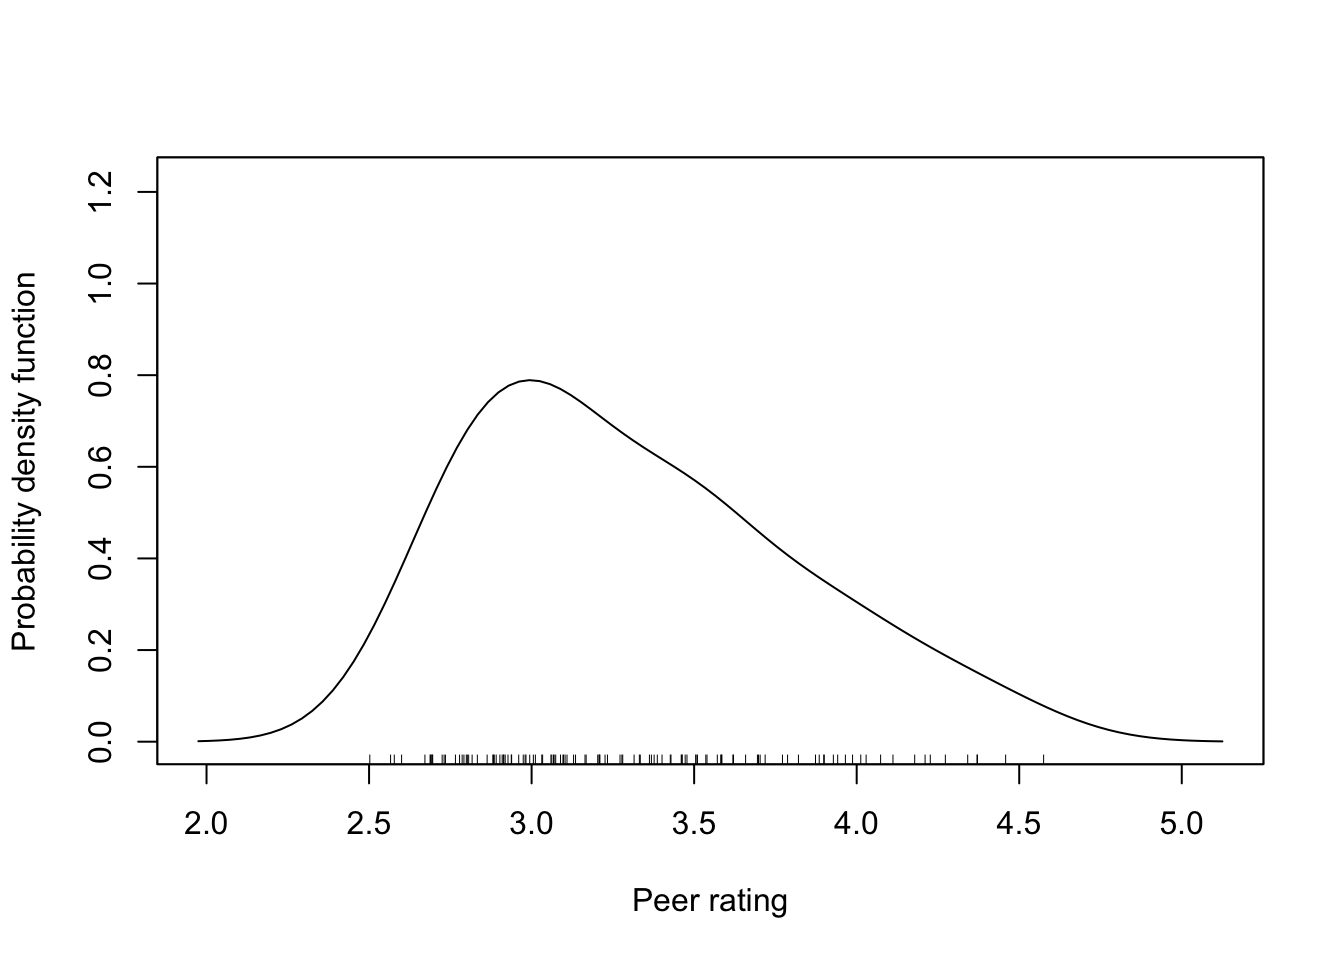
\includegraphics[width=0.5\linewidth]{epsy-8252-notes_files/figure-latex/unnamed-chunk-147-1} 

}

\caption{Density plot of the outcome variable used in the different models.}\label{fig:unnamed-chunk-147}
\end{figure}

Below we show scatterplots of the outcome (peer ratings) versus each of the predictors we are considering in the three scientific models.

\begin{figure}

{\centering 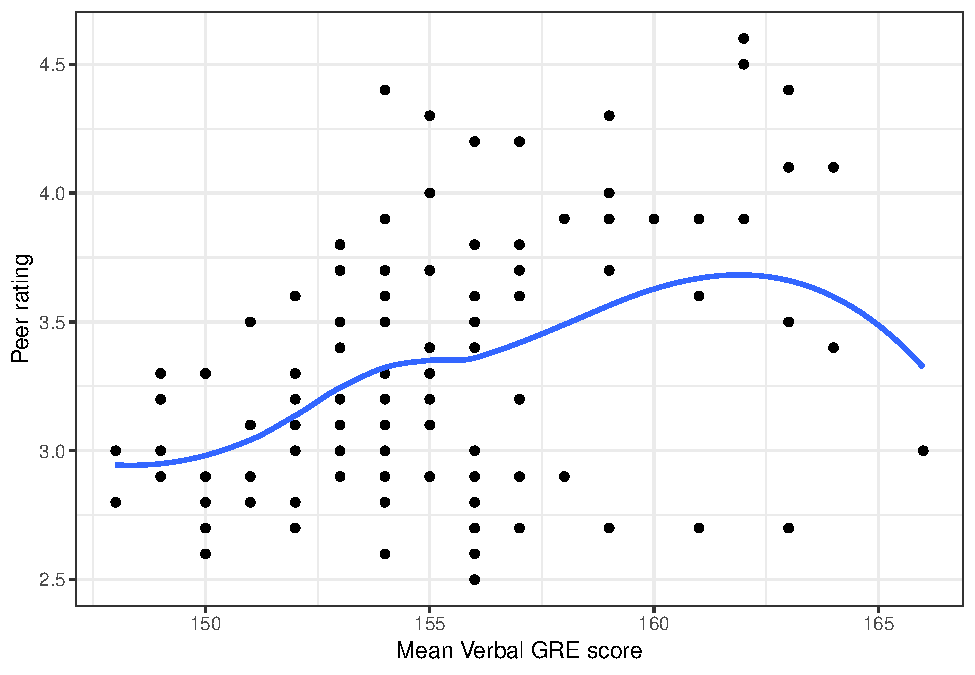
\includegraphics[width=0.4\linewidth]{epsy-8252-notes_files/figure-latex/unnamed-chunk-148-1} 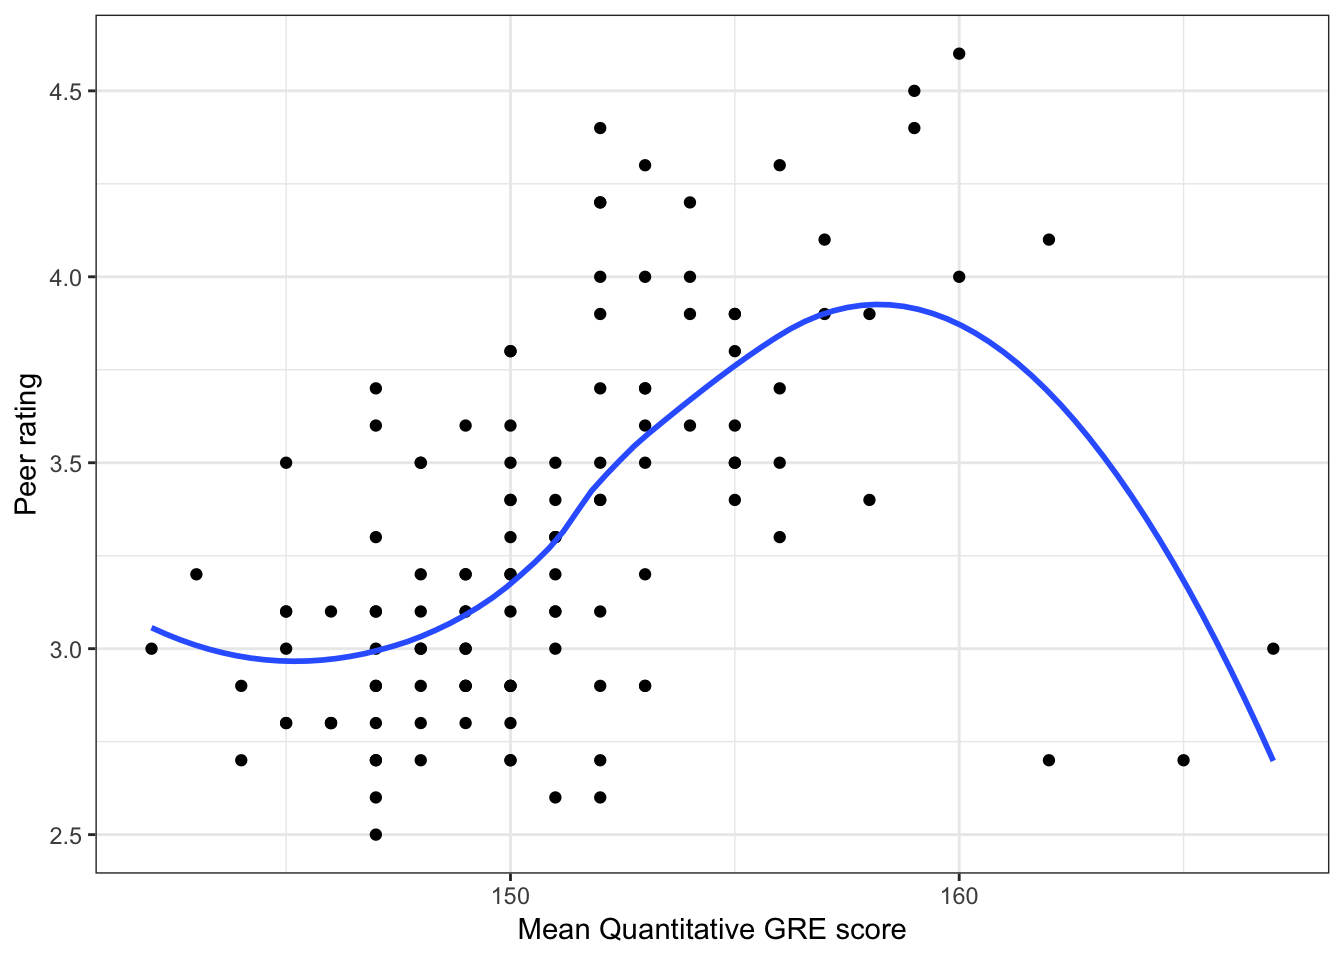
\includegraphics[width=0.4\linewidth]{epsy-8252-notes_files/figure-latex/unnamed-chunk-148-2} 

}

\caption{Scatterplots of peer ratings versus the student-related factors; verbal and quantitative GRE scores. The loess smoother is also displayed.}\label{fig:unnamed-chunk-148}
\end{figure}

\begin{figure}

{\centering 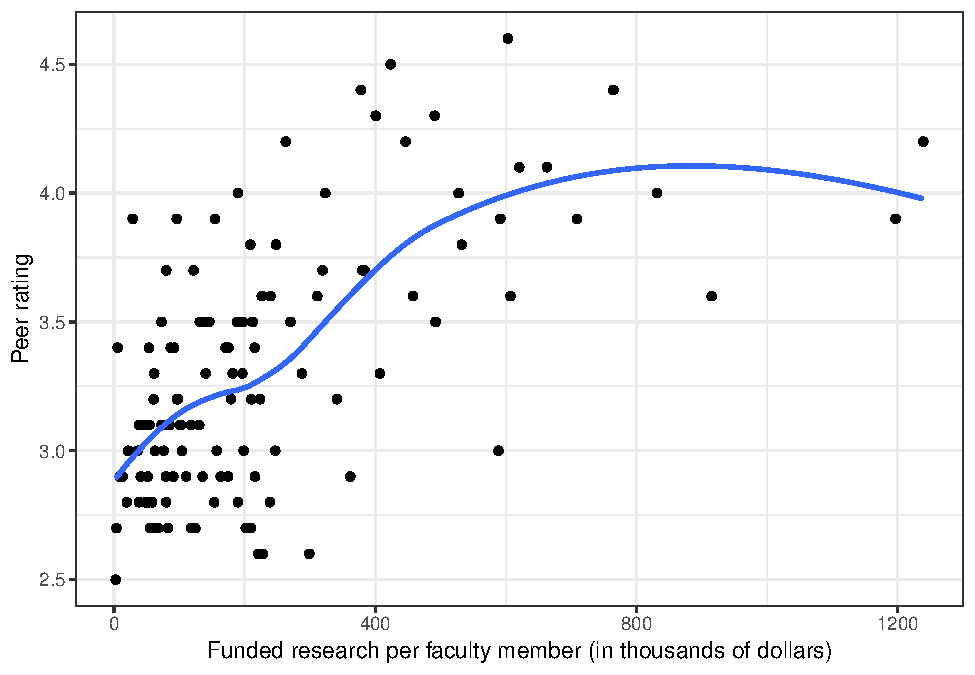
\includegraphics[width=0.4\linewidth]{epsy-8252-notes_files/figure-latex/unnamed-chunk-149-1} 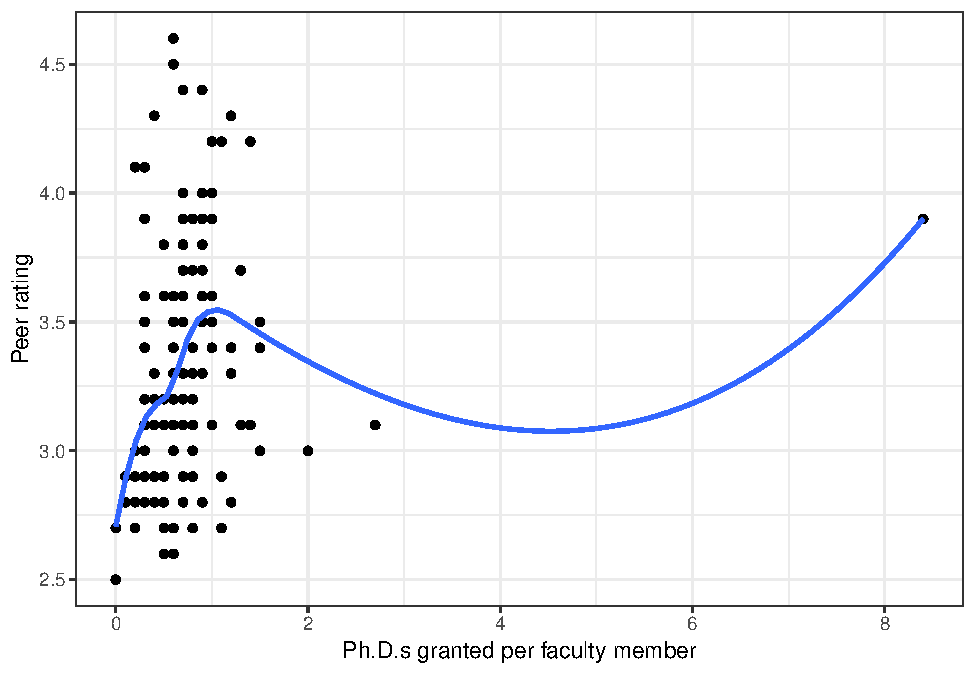
\includegraphics[width=0.4\linewidth]{epsy-8252-notes_files/figure-latex/unnamed-chunk-149-2} 

}

\caption{Scatterplots of peer ratings versus the faculty-related factors; funded research (per faculty member) and number of Ph.D.s granted (per faculty member). The loess smoother is also displayed.}\label{fig:unnamed-chunk-149}
\end{figure}

\begin{figure}

{\centering 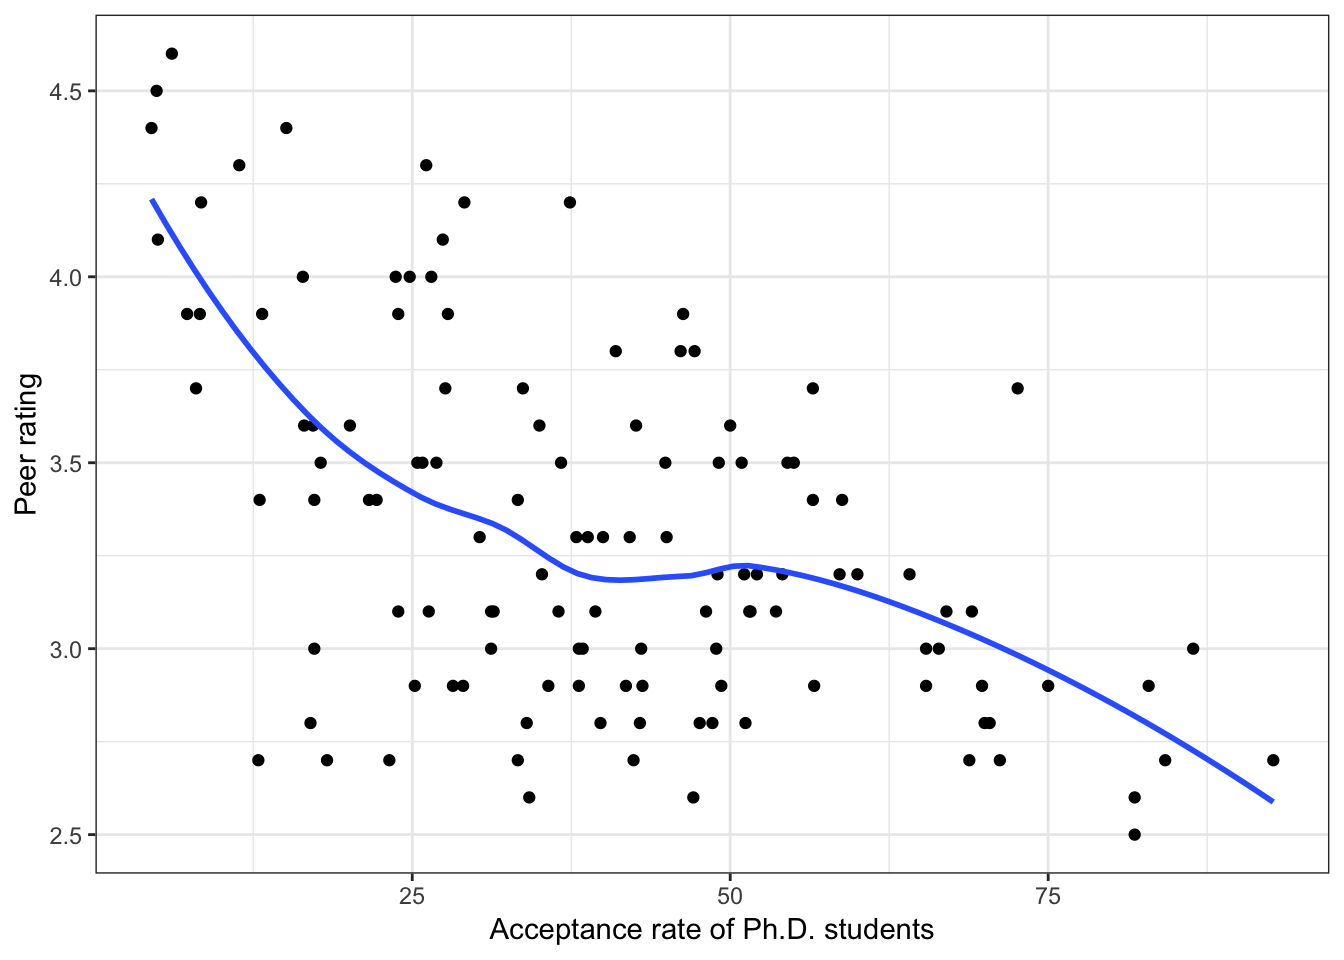
\includegraphics[width=0.3\linewidth]{epsy-8252-notes_files/figure-latex/unnamed-chunk-150-1} 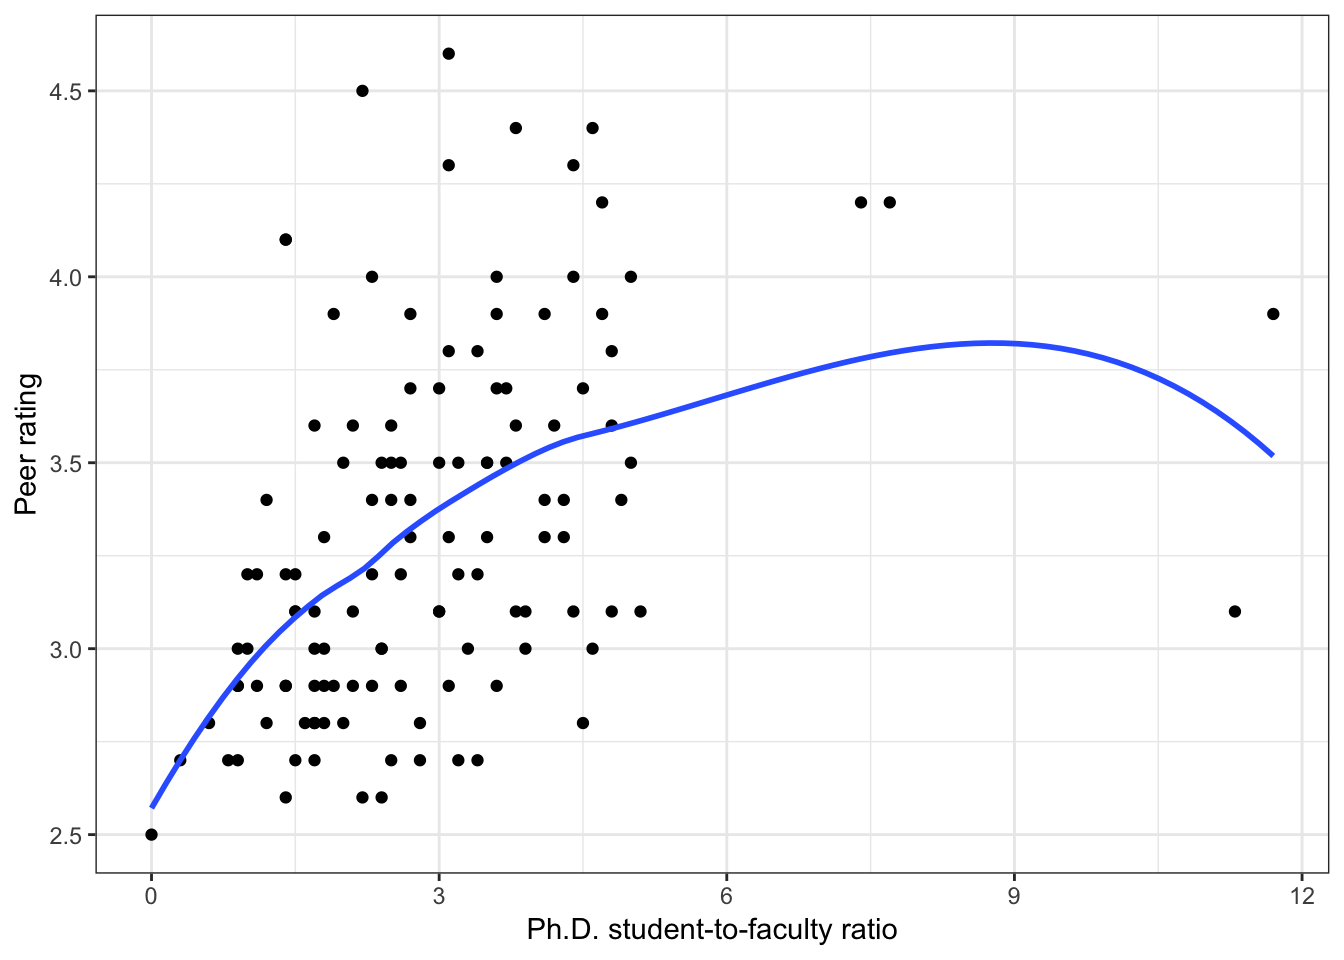
\includegraphics[width=0.3\linewidth]{epsy-8252-notes_files/figure-latex/unnamed-chunk-150-2} 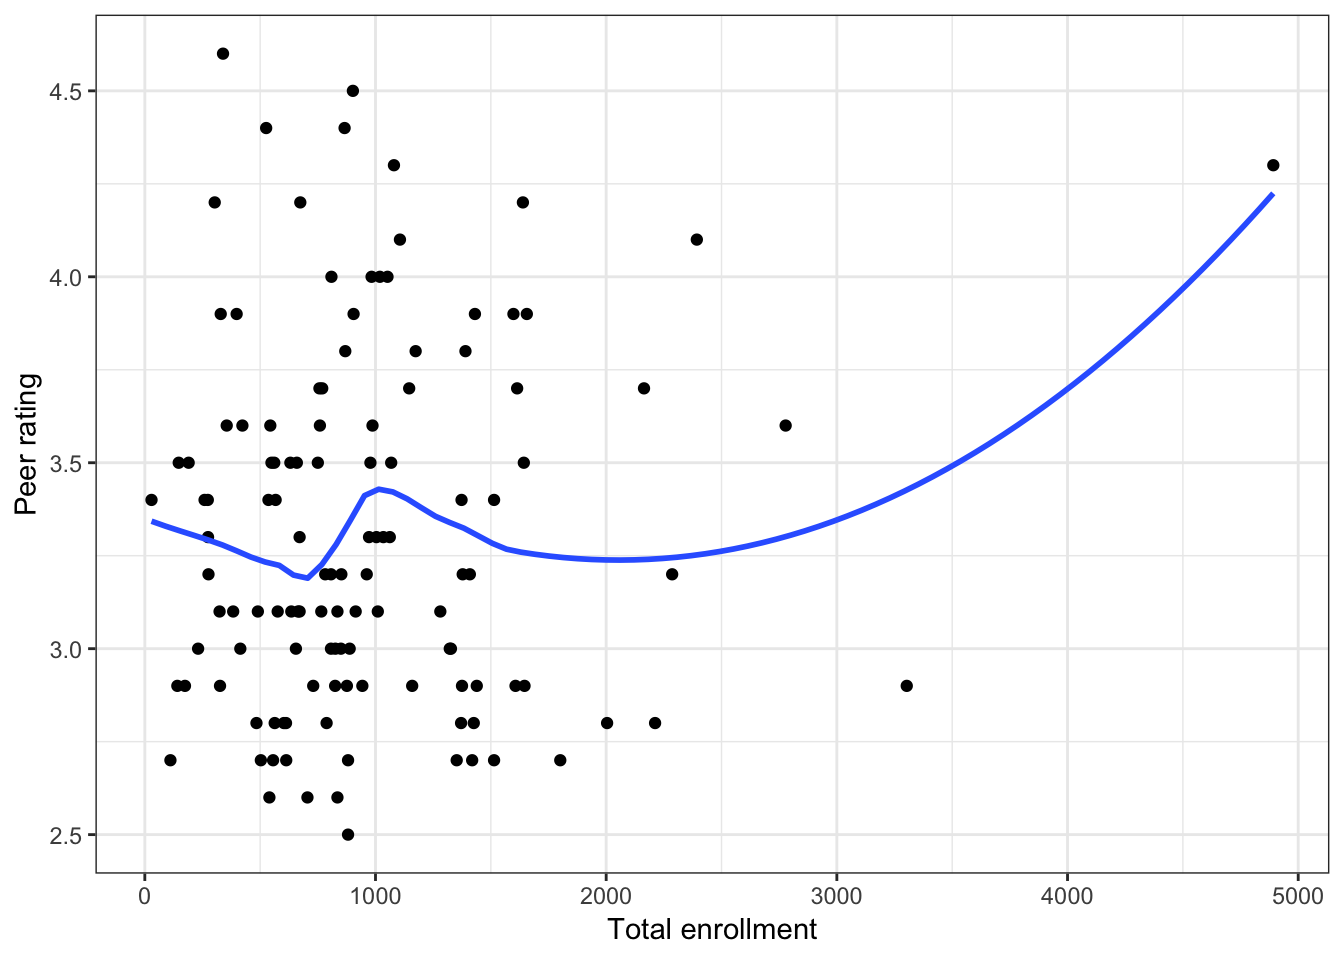
\includegraphics[width=0.3\linewidth]{epsy-8252-notes_files/figure-latex/unnamed-chunk-150-3} 

}

\caption{Scatterplots of peer ratings versus the institution-related factors; acceptance rate of Ph.D. students, the Ph.D. student-to-faculty ratio, and the size of the program. The loess smoother is also displayed.}\label{fig:unnamed-chunk-150}
\end{figure}

Almost all of these plots show curvilinear patterns, some of which can be alleviated by log-transforming the outcome. Remember, log-transforming the outcome will also help with violations of homoskedasticity. Since we want to be able to compare the models at the end of the analysis, we NEED to use the same outcome in each of the models. Given the initial right-skewed nature of the outcome distribution and the evidence from the scatterplots, we will log-transform peer ratings and use that outcome in each model we fit.

\begin{Shaded}
\begin{Highlighting}[]
\CommentTok{# Create log-transformed peer ratings}
\NormalTok{educ =}\StringTok{ }\NormalTok{educ }\OperatorTok
\StringTok{  }\KeywordTok{mutate}\NormalTok{(}
    \DataTypeTok{Lpeer =} \KeywordTok{log}\NormalTok{(peer)}
\NormalTok{    )}
\end{Highlighting}
\end{Shaded}

\hypertarget{building-the-student-related-factors-model}{%
\subsection{Building the Student-Related Factors Model}\label{building-the-student-related-factors-model}}

To determine which of the student-related factors to include in the model, we will examine the scatterplots of each predictor against the log-transformed peer ratings and also examine the correlation matrix of the outcome and student-related predictors.

\begin{figure}

{\centering 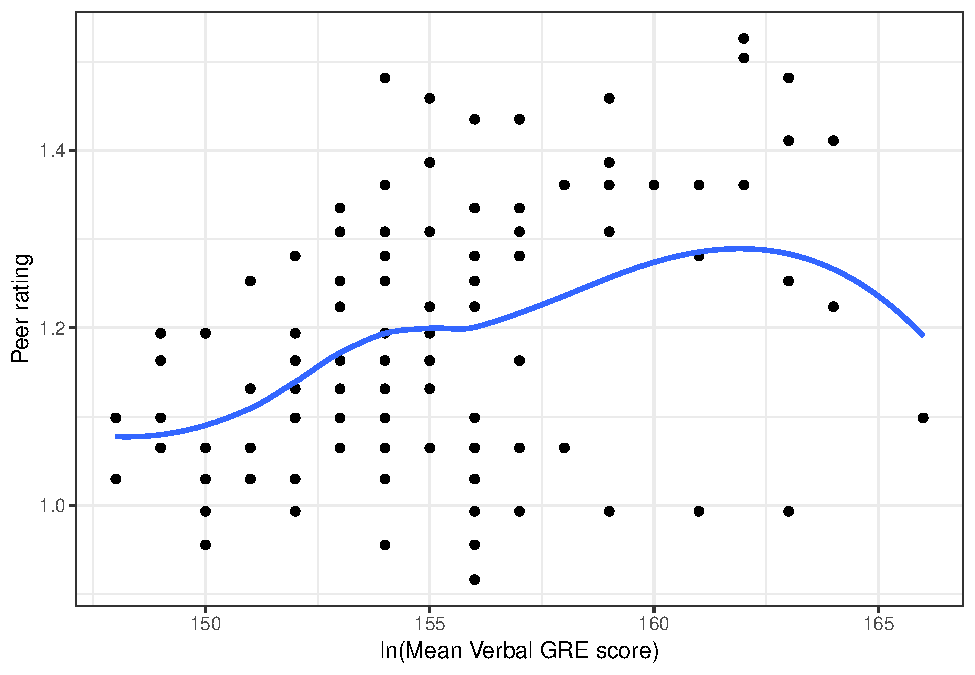
\includegraphics[width=0.4\linewidth]{epsy-8252-notes_files/figure-latex/unnamed-chunk-152-1} 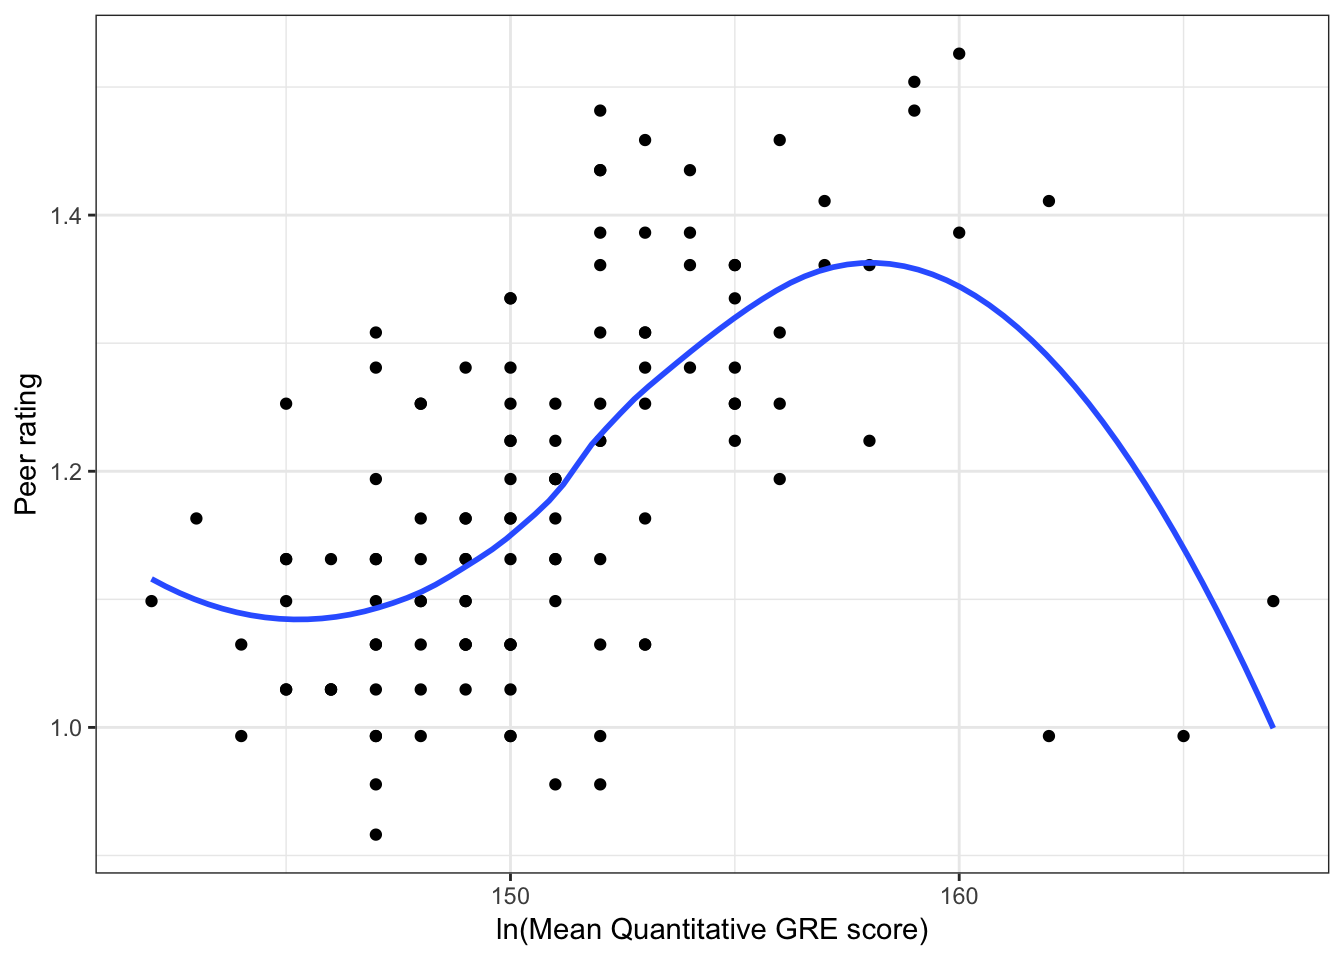
\includegraphics[width=0.4\linewidth]{epsy-8252-notes_files/figure-latex/unnamed-chunk-152-2} 

}

\caption{Scatterplots of the log-transformed peer ratings versus the student-related factors; verbal and quantitative GRE scores. The loess smoother is also displayed.}\label{fig:unnamed-chunk-152}
\end{figure}

\begin{Shaded}
\begin{Highlighting}[]
\NormalTok{educ }\OperatorTok
\StringTok{  }\KeywordTok{select}\NormalTok{(Lpeer, gre_verbal, gre_quant) }\OperatorTok
\StringTok{  }\KeywordTok{correlate}\NormalTok{()}
\end{Highlighting}
\end{Shaded}

\begin{verbatim}
# A tibble: 3 x 4
  rowname     Lpeer gre_verbal gre_quant
  <chr>       <dbl>      <dbl>     <dbl>
1 Lpeer      NA          0.408     0.478
2 gre_verbal  0.408     NA         0.808
3 gre_quant   0.478      0.808    NA    
\end{verbatim}

Not surprisingly, the mean GRE verbal and GRE quantitative scores are highly correlated. Since including highly correlated predictors in a model can lead to unstable estimates, we will drop one of the predictors from the model. Empirically, the quantitative GRE scores seem more highly correlated with the outcome, so we will drop the GRE verbal scores from the model.

Focusing on the scatterplot of the GRE quantitative scores, the relationship with the log-transformed peer ratings looks curvilinear (non-monotonic). The empirical relationship seems to change direction twice, indicating that log-transformed peer ratings may be a cubic-function of the quantitative GRE scores.

\begin{Shaded}
\begin{Highlighting}[]
\CommentTok{# Fit cubic model}
\NormalTok{lm}\FloatTok{.1}\NormalTok{ =}\StringTok{ }\KeywordTok{lm}\NormalTok{(Lpeer }\OperatorTok{~}\StringTok{ }\DecValTok{1} \OperatorTok{+}\StringTok{ }\NormalTok{gre_quant }\OperatorTok{+}\StringTok{ }\KeywordTok{I}\NormalTok{(gre_quant}\OperatorTok{^}\DecValTok{2}\NormalTok{) }\OperatorTok{+}\StringTok{ }\KeywordTok{I}\NormalTok{(gre_quant}\OperatorTok{^}\DecValTok{3}\NormalTok{), }\DataTypeTok{data =}\NormalTok{ educ)}

\CommentTok{# Coefficient-level output}
\KeywordTok{tidy}\NormalTok{(lm}\FloatTok{.1}\NormalTok{)}
\end{Highlighting}
\end{Shaded}

\begin{verbatim}
# A tibble: 4 x 5
  term              estimate   std.error statistic   p.value
  <chr>                <dbl>       <dbl>     <dbl>     <dbl>
1 (Intercept)     780.       176.             4.43 0.0000210
2 gre_quant       -15.4        3.43          -4.49 0.0000165
3 I(gre_quant^2)    0.102      0.0223         4.55 0.0000129
4 I(gre_quant^3)   -0.000223   0.0000483     -4.61 0.0000102
\end{verbatim}

\begin{Shaded}
\begin{Highlighting}[]
\CommentTok{# Obtain residuals}
\NormalTok{out_}\DecValTok{1}\NormalTok{ =}\StringTok{ }\KeywordTok{augment}\NormalTok{(lm}\FloatTok{.1}\NormalTok{)}

\CommentTok{# Examine residuals}
\KeywordTok{sm.density}\NormalTok{(out_}\DecValTok{1}\OperatorTok{$}\NormalTok{.std.resid, }\DataTypeTok{xlab =} \StringTok{"Standardized residuals"}\NormalTok{, }\DataTypeTok{model =} \StringTok{"normal"}\NormalTok{)}

\KeywordTok{ggplot}\NormalTok{(}\DataTypeTok{data =}\NormalTok{ out_}\DecValTok{1}\NormalTok{, }\KeywordTok{aes}\NormalTok{(}\DataTypeTok{x =}\NormalTok{ .fitted, }\DataTypeTok{y =}\NormalTok{ .std.resid)) }\OperatorTok{+}
\StringTok{  }\KeywordTok{geom_point}\NormalTok{() }\OperatorTok{+}
\StringTok{  }\KeywordTok{geom_hline}\NormalTok{(}\DataTypeTok{yintercept =} \DecValTok{0}\NormalTok{) }\OperatorTok{+}
\StringTok{  }\KeywordTok{theme_bw}\NormalTok{() }\OperatorTok{+}
\StringTok{  }\KeywordTok{xlab}\NormalTok{(}\StringTok{"Fitted values"}\NormalTok{) }\OperatorTok{+}
\StringTok{  }\KeywordTok{ylab}\NormalTok{(}\StringTok{"Standardized residuals"}\NormalTok{)}
\end{Highlighting}
\end{Shaded}

\begin{figure}

{\centering 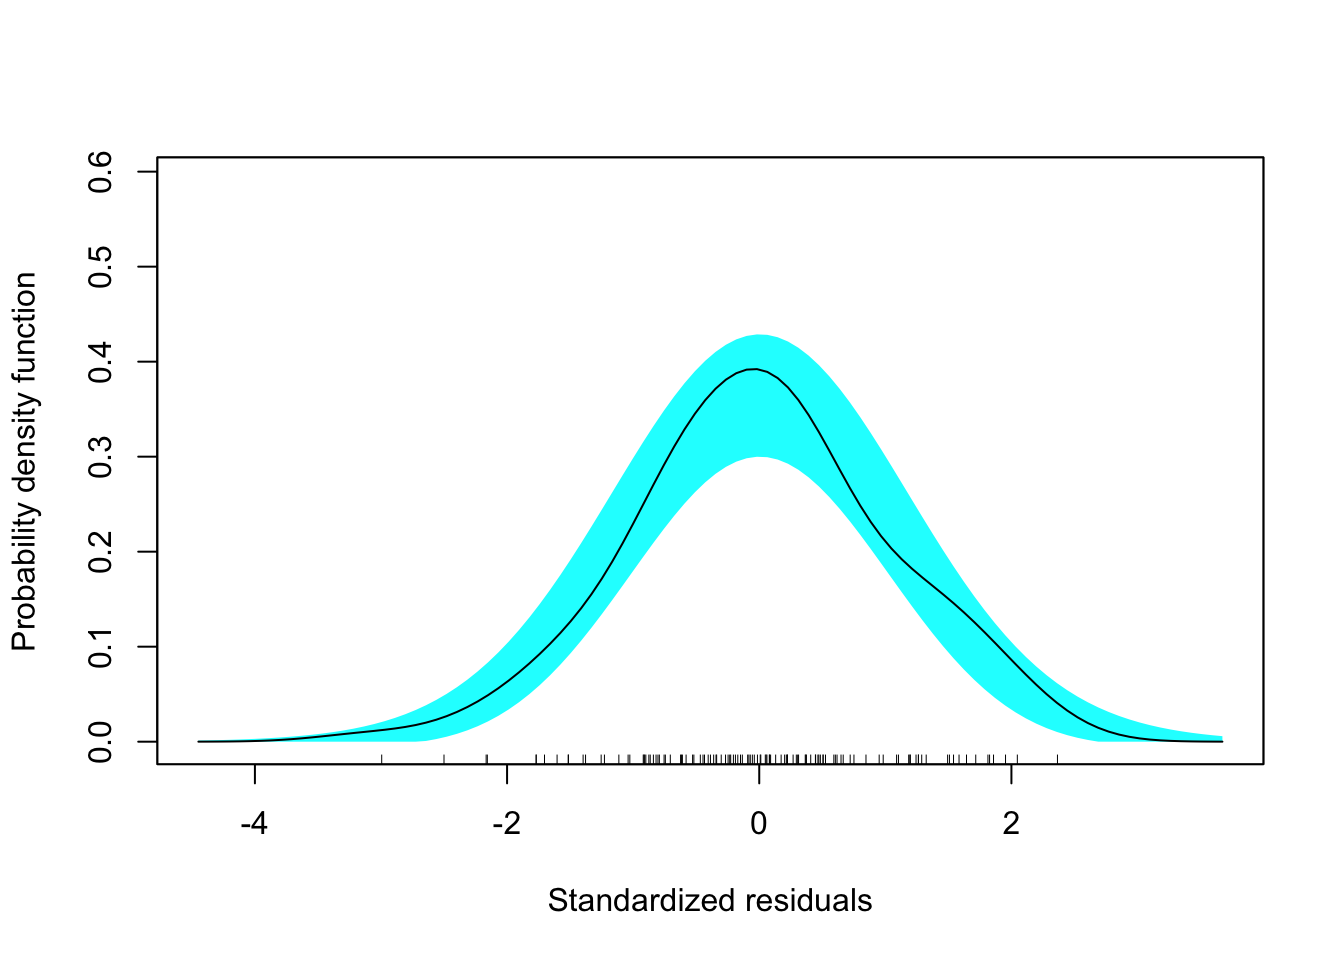
\includegraphics[width=0.4\linewidth]{epsy-8252-notes_files/figure-latex/unnamed-chunk-154-1} 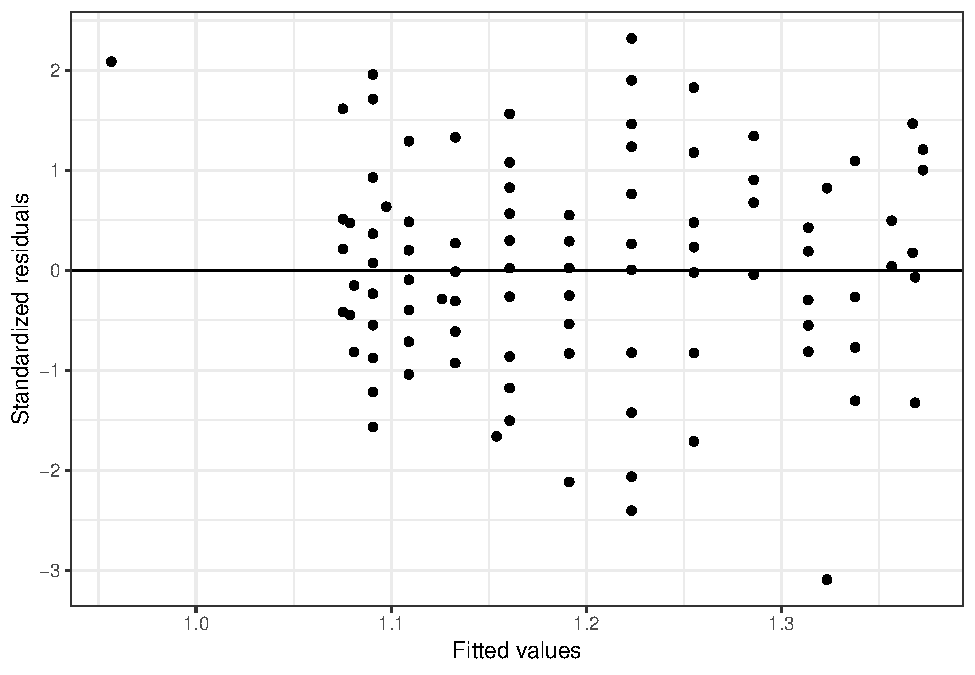
\includegraphics[width=0.4\linewidth]{epsy-8252-notes_files/figure-latex/unnamed-chunk-154-2} 

}

\caption{Residual plots for the fitted model using the student-related factors.}\label{fig:unnamed-chunk-154}
\end{figure}

\hypertarget{building-the-faculty-related-factors-model}{%
\subsection{Building the Faculty-Related Factors Model}\label{building-the-faculty-related-factors-model}}

To determine which of the faculty-related factors to include in the model, we will examine the scatterplots of each predictor against the log-transformed peer ratings and also examine the correlation matrix of the outcome and faculty-related predictors.

\begin{figure}

{\centering 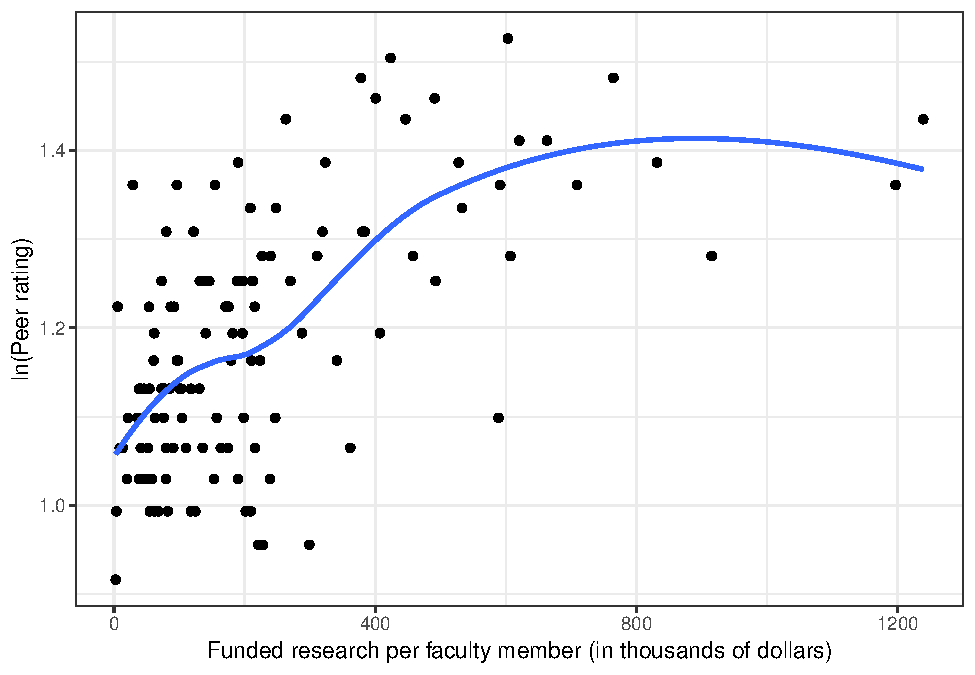
\includegraphics[width=0.4\linewidth]{epsy-8252-notes_files/figure-latex/unnamed-chunk-155-1} 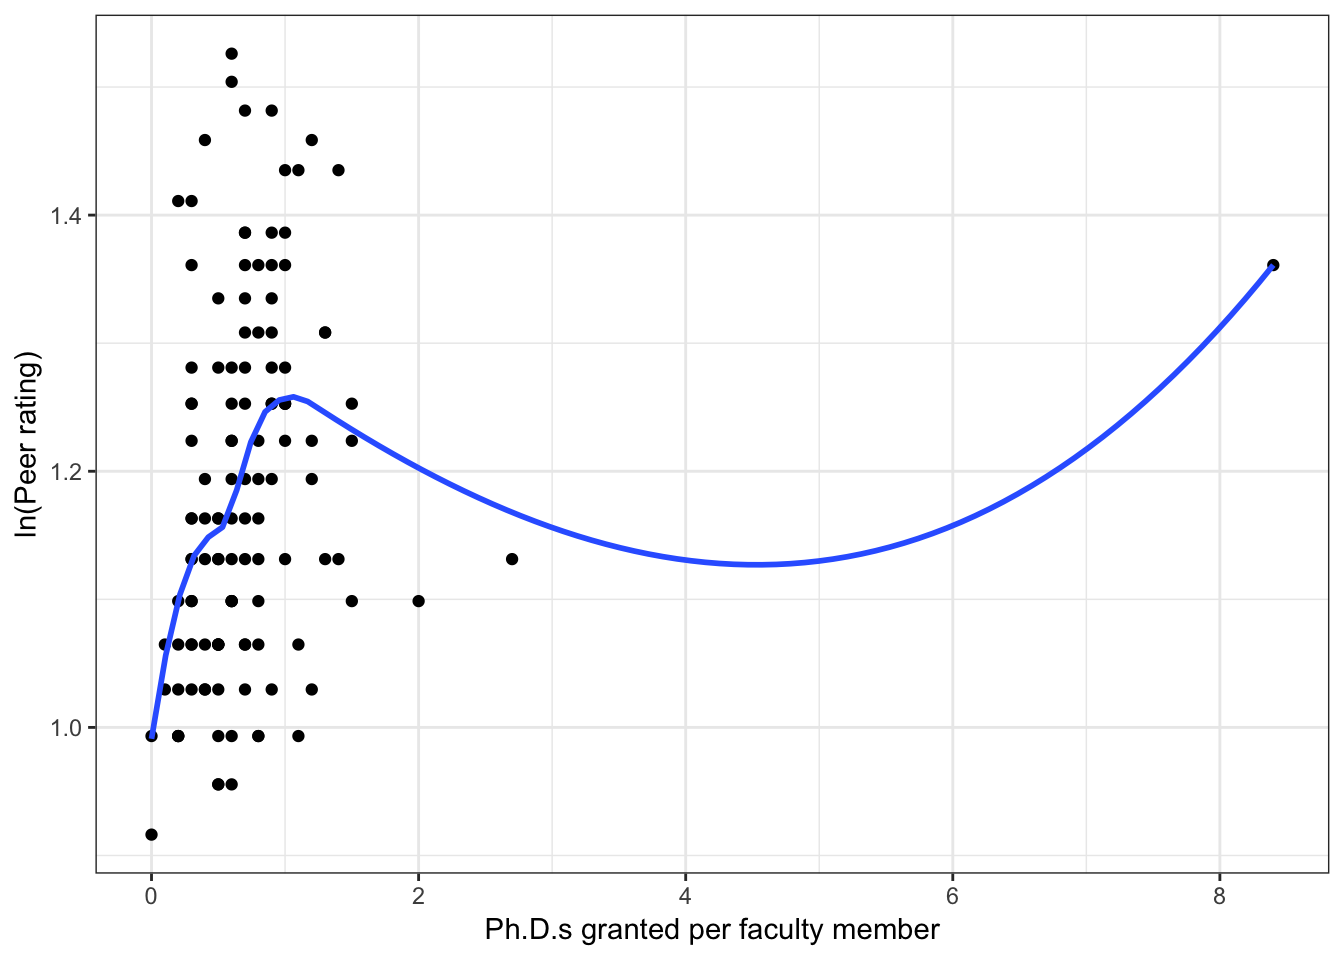
\includegraphics[width=0.4\linewidth]{epsy-8252-notes_files/figure-latex/unnamed-chunk-155-2} 

}

\caption{Scatterplots of log-transformed peer ratings versus the faculty-related factors; funded research (per faculty member) and number of Ph.D.s granted (per faculty member). The loess smoother is also displayed.}\label{fig:unnamed-chunk-155}
\end{figure}

\begin{Shaded}
\begin{Highlighting}[]
\NormalTok{educ }\OperatorTok
\StringTok{  }\KeywordTok{select}\NormalTok{(Lpeer, funded_research_per_faculty, phd_granted_per_faculty) }\OperatorTok
\StringTok{  }\KeywordTok{correlate}\NormalTok{()}
\end{Highlighting}
\end{Shaded}

\begin{verbatim}
# A tibble: 3 x 4
  rowname                Lpeer funded_research_per_fa~ phd_granted_per_fac~
  <chr>                  <dbl>                   <dbl>                <dbl>
1 Lpeer                 NA                       0.597                0.217
2 funded_research_per_~  0.597                  NA                    0.403
3 phd_granted_per_facu~  0.217                   0.403               NA    
\end{verbatim}

The two predictors are moderately correlated with each other and both are correlated with the outcome. The scatterplot of peer ratings versus funded research suggest a monotonic curvilinear relationship. The Rule of the Bulge indicates that log-transforming the predictor may help linearize this relationship. The scatterplot of peer ratings versus number of Ph.D.s granted suggests that the distribution of the predictor is right-skewed with a potential outlying observation. This relationship may also benefit from log-transforming the predictor.

Before log-transforming these predictors, it is a good idea to check the distributions for zero or negative values.

\begin{Shaded}
\begin{Highlighting}[]
\NormalTok{educ }\OperatorTok
\StringTok{  }\KeywordTok{select}\NormalTok{(funded_research_per_faculty, phd_granted_per_faculty) }\OperatorTok
\StringTok{  }\KeywordTok{summary}\NormalTok{()}
\end{Highlighting}
\end{Shaded}

\begin{verbatim}
 funded_research_per_faculty phd_granted_per_faculty
 Min.   :   2.9              Min.   :0.000          
 1st Qu.:  77.8              1st Qu.:0.400          
 Median : 160.6              Median :0.650          
 Mean   : 228.8              Mean   :0.758          
 3rd Qu.: 283.4              3rd Qu.:0.900          
 Max.   :1239.1              Max.   :8.400          
\end{verbatim}

The summary values for the \texttt{phd\_granted\_per\_faculty} predictor indicates that there are some schools that have a value of 0 for this predictor and that 0 is the smallest value. Before we transform using a log-transformation, we need to make it so the smallest value in the predictor is 1, since the log of 0 (and any negative values) is undefined. To do this we will add some number (in our case 1) to each value for \texttt{phd\_granted\_per\_faculty} prior to taking the log.

\begin{Shaded}
\begin{Highlighting}[]
\CommentTok{#Create log of the faculty-related predictors}
\NormalTok{educ =}\StringTok{ }\NormalTok{educ }\OperatorTok
\StringTok{  }\KeywordTok{mutate}\NormalTok{(}
    \DataTypeTok{Lfunded_research_per_faculty =} \KeywordTok{log}\NormalTok{(funded_research_per_faculty),}
    \DataTypeTok{Lphd_granted_per_faculty =} \KeywordTok{log}\NormalTok{(phd_granted_per_faculty }\OperatorTok{+}\StringTok{ }\DecValTok{1}\NormalTok{)}
\NormalTok{  )}
\end{Highlighting}
\end{Shaded}

\begin{figure}

{\centering 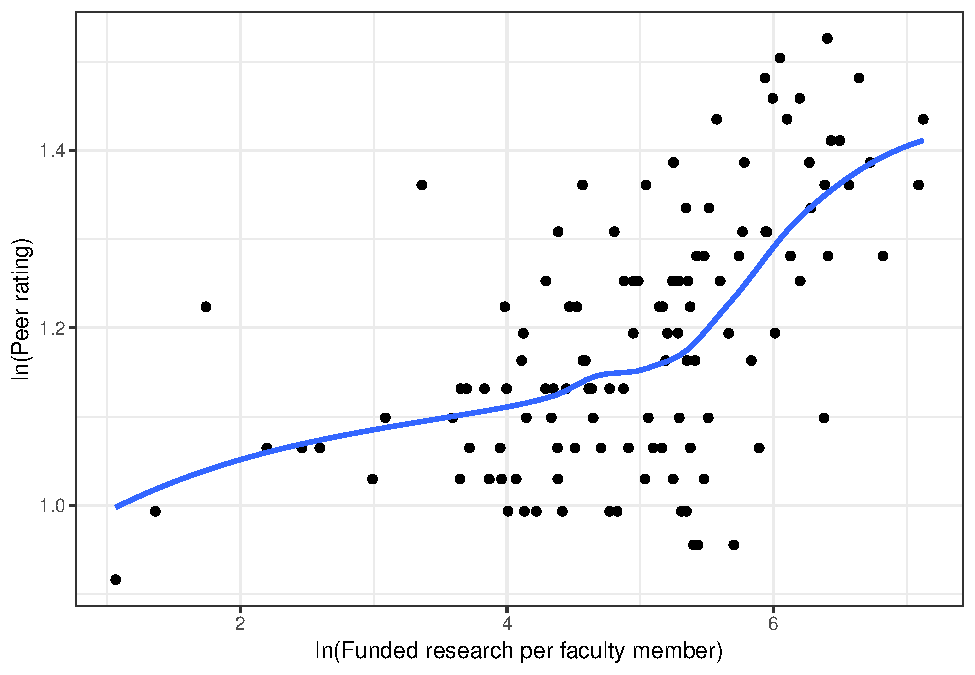
\includegraphics[width=0.4\linewidth]{epsy-8252-notes_files/figure-latex/unnamed-chunk-159-1} 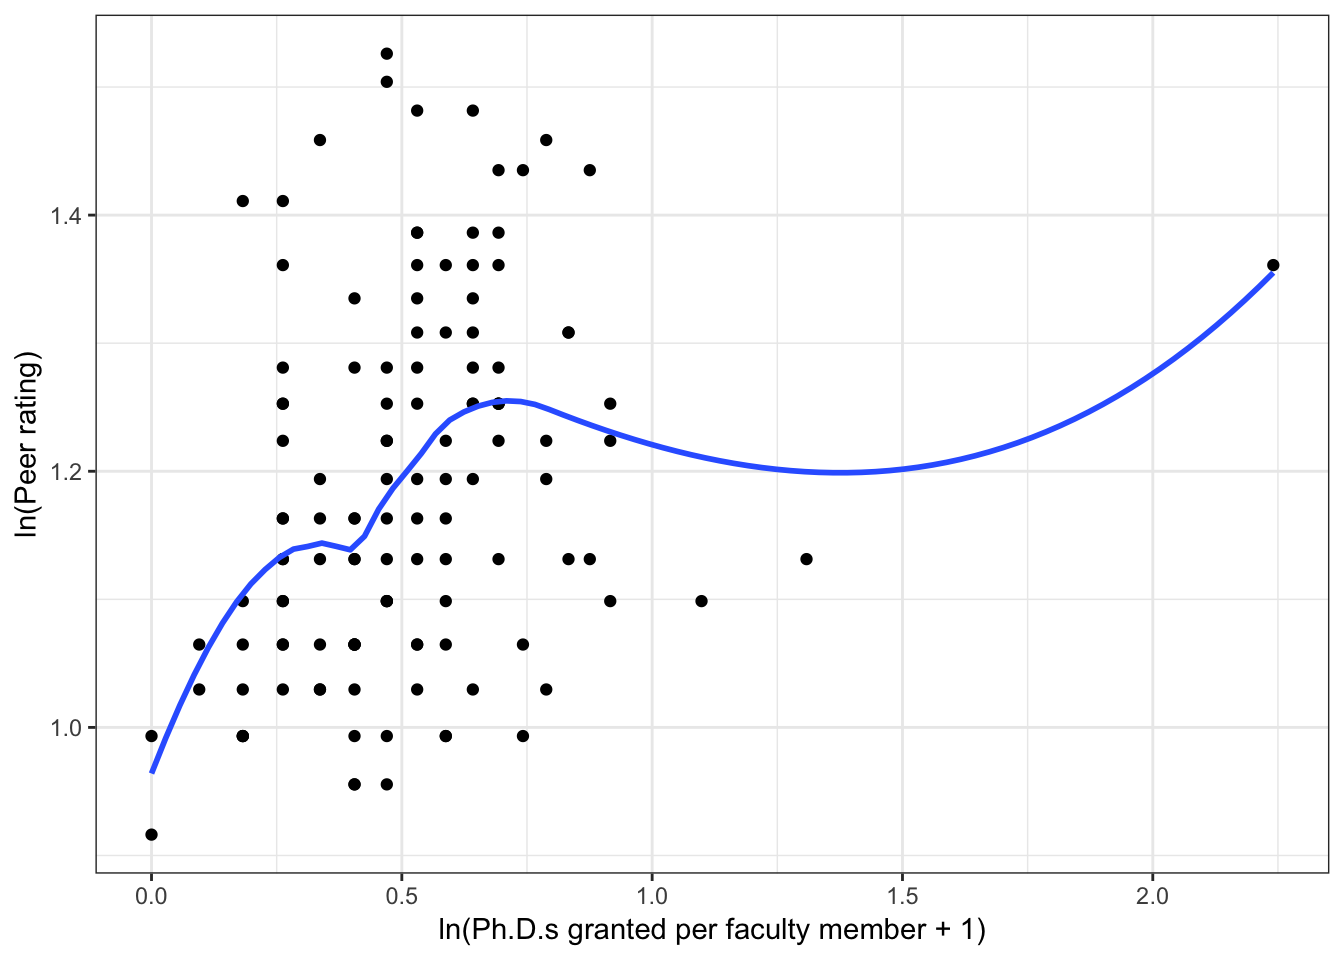
\includegraphics[width=0.4\linewidth]{epsy-8252-notes_files/figure-latex/unnamed-chunk-159-2} 

}

\caption{Scatterplots of log-transformed peer ratings versus the log-transformed faculty-related factors; funded research (per faculty member) and number of Ph.D.s granted (per faculty member). The loess smoother is also displayed.}\label{fig:unnamed-chunk-159}
\end{figure}

Although this helped, it did not ``cure'' the nonlinearity. We might want to further include a quadratic term for each of the predictors. To evaluate this, we will fit the model that includes the linear and quadratic log-transformed predictors and examine the coefficient-level output and residuals.

\begin{Shaded}
\begin{Highlighting}[]
\CommentTok{# Fit model}
\NormalTok{lm}\FloatTok{.2}\NormalTok{ =}\StringTok{ }\KeywordTok{lm}\NormalTok{(Lpeer }\OperatorTok{~}\StringTok{ }\DecValTok{1} \OperatorTok{+}\StringTok{ }\NormalTok{Lfunded_research_per_faculty }\OperatorTok{+}\StringTok{ }\KeywordTok{I}\NormalTok{(Lfunded_research_per_faculty}\OperatorTok{^}\DecValTok{2}\NormalTok{) }\OperatorTok{+}\StringTok{ }\NormalTok{Lphd_granted_per_faculty  }\OperatorTok{+}\StringTok{ }\KeywordTok{I}\NormalTok{(Lphd_granted_per_faculty}\OperatorTok{^}\DecValTok{2}\NormalTok{), }\DataTypeTok{data =}\NormalTok{ educ)}

\CommentTok{# Coefficient-level output}
\KeywordTok{tidy}\NormalTok{(lm}\FloatTok{.2}\NormalTok{)}
\end{Highlighting}
\end{Shaded}

\begin{verbatim}
# A tibble: 5 x 5
  term                              estimate std.error statistic  p.value
  <chr>                                <dbl>     <dbl>     <dbl>    <dbl>
1 (Intercept)                         1.21     0.106       11.5  6.76e-21
2 Lfunded_research_per_faculty       -0.151    0.0509      -2.96 3.70e- 3
3 I(Lfunded_research_per_faculty^2)   0.0238   0.00547      4.35 2.87e- 5
4 Lphd_granted_per_faculty            0.300    0.0948       3.16 1.99e- 3
5 I(Lphd_granted_per_faculty^2)      -0.139    0.0503      -2.77 6.58e- 3
\end{verbatim}

\begin{Shaded}
\begin{Highlighting}[]
\CommentTok{# Obtain residuals}
\NormalTok{out_}\DecValTok{2}\NormalTok{ =}\StringTok{ }\KeywordTok{augment}\NormalTok{(lm}\FloatTok{.1}\NormalTok{)}

\CommentTok{# Examine residuals}
\KeywordTok{sm.density}\NormalTok{(out_}\DecValTok{2}\OperatorTok{$}\NormalTok{.std.resid, }\DataTypeTok{xlab =} \StringTok{"Standardized residuals"}\NormalTok{, }\DataTypeTok{model =} \StringTok{"normal"}\NormalTok{)}

\KeywordTok{ggplot}\NormalTok{(}\DataTypeTok{data =}\NormalTok{ out_}\DecValTok{2}\NormalTok{, }\KeywordTok{aes}\NormalTok{(}\DataTypeTok{x =}\NormalTok{ .fitted, }\DataTypeTok{y =}\NormalTok{ .std.resid)) }\OperatorTok{+}
\StringTok{  }\KeywordTok{geom_point}\NormalTok{() }\OperatorTok{+}
\StringTok{  }\KeywordTok{geom_hline}\NormalTok{(}\DataTypeTok{yintercept =} \DecValTok{0}\NormalTok{) }\OperatorTok{+}
\StringTok{  }\KeywordTok{theme_bw}\NormalTok{() }\OperatorTok{+}
\StringTok{  }\KeywordTok{xlab}\NormalTok{(}\StringTok{"Fitted values"}\NormalTok{) }\OperatorTok{+}
\StringTok{  }\KeywordTok{ylab}\NormalTok{(}\StringTok{"Standardized residuals"}\NormalTok{)}
\end{Highlighting}
\end{Shaded}

\begin{figure}

{\centering 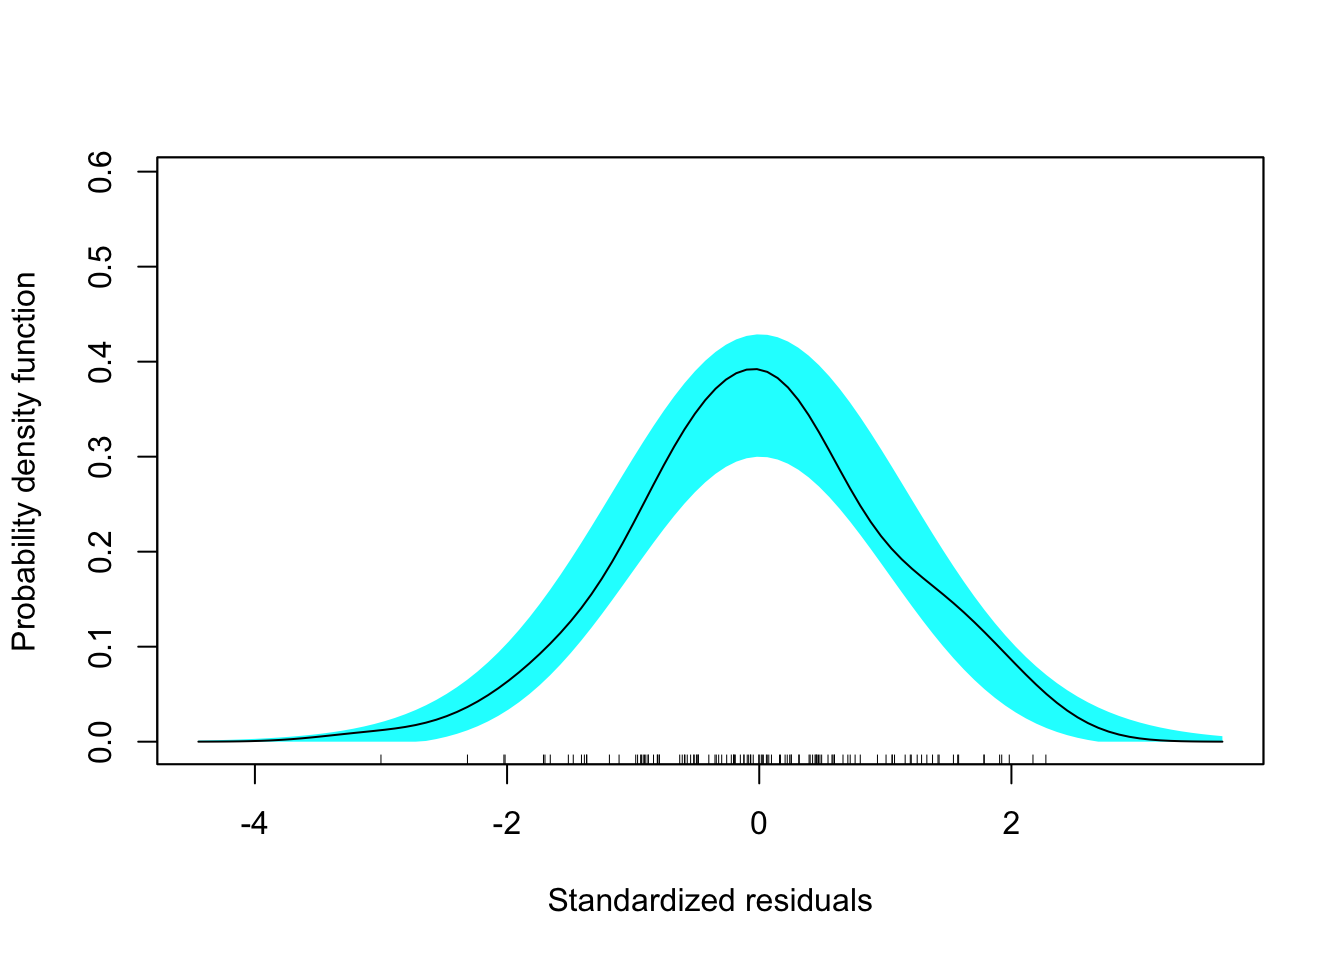
\includegraphics[width=0.4\linewidth]{epsy-8252-notes_files/figure-latex/unnamed-chunk-160-1} \includegraphics[width=0.4\linewidth]{epsy-8252-notes_files/figure-latex/unnamed-chunk-160-2} 

}

\caption{Residual plots for the fitted model using the faculty-related factors.}\label{fig:unnamed-chunk-160}
\end{figure}

\hypertarget{building-the-institution-related-factors-model}{%
\subsection{Building the Institution-Related Factors Model}\label{building-the-institution-related-factors-model}}

To determine which of the institution-related factors to include in the model, we will examine the scatterplots of each predictor against the log-transformed peer ratings and also examine the correlation matrix of the outcome and institution-related predictors.

\begin{figure}

{\centering \includegraphics[width=0.3\linewidth]{epsy-8252-notes_files/figure-latex/unnamed-chunk-161-1} \includegraphics[width=0.3\linewidth]{epsy-8252-notes_files/figure-latex/unnamed-chunk-161-2} \includegraphics[width=0.3\linewidth]{epsy-8252-notes_files/figure-latex/unnamed-chunk-161-3} 

}

\caption{Scatterplots of the log-transformed peer ratings versus the institution-related factors; acceptance rate of Ph.D. students, the Ph.D. student-to-faculty ratio, and the size of the program. The loess smoother is also displayed.}\label{fig:unnamed-chunk-161}
\end{figure}

\begin{Shaded}
\begin{Highlighting}[]
\NormalTok{educ }\OperatorTok
\StringTok{  }\KeywordTok{select}\NormalTok{(Lpeer, doc_accept, phd_student_faculty_ratio, enroll) }\OperatorTok
\StringTok{  }\KeywordTok{correlate}\NormalTok{()}
\end{Highlighting}
\end{Shaded}

\begin{verbatim}
# A tibble: 4 x 5
  rowname                 Lpeer doc_accept phd_student_faculty_r~    enroll
  <chr>                   <dbl>      <dbl>                  <dbl>     <dbl>
1 Lpeer                 NA         -0.534                 0.423     0.0964 
2 doc_accept            -0.534     NA                    -0.235    -0.0256 
3 phd_student_faculty~   0.423     -0.235                NA         0.00450
4 enroll                 0.0964    -0.0256                0.00450  NA      
\end{verbatim}

The three predictors are mostly uncorrelated with each other and all are correlated with the outcome, albeit enrollment is weakly correlated with peer ratings. Two of the three scatterplots suggest curvilinear relationships although with different functional forms---Ph.D.~student-to-faculty ratio and total enrollment. The Rule of the Bulge indicates that log-transforming the Ph.D.~student-to-faculty ratio predictor, and including quadratic may help linearize this relationship. The scatterplot of peer ratings versus total enrollment suggests that the distribution of the predictor is right-skewed with a potential outlying observations. This relationship may also benefit from log-transforming the predictor. Lastly, it is unclear whether any additional transformation or polynomial terms are necessary for modeling the relationship with doctoral acceptance rate; to double-check this we will also log-transform the total enrollment predictor.

As before, prior to log-transforming any predictors, it is a good idea to check the distributions for zero or negative values.

\begin{Shaded}
\begin{Highlighting}[]
\NormalTok{educ }\OperatorTok
\StringTok{  }\KeywordTok{select}\NormalTok{(doc_accept, phd_student_faculty_ratio, enroll) }\OperatorTok
\StringTok{  }\KeywordTok{summary}\NormalTok{()}
\end{Highlighting}
\end{Shaded}

\begin{verbatim}
   doc_accept   phd_student_faculty_ratio     enroll    
 Min.   : 4.5   Min.   : 0.00             Min.   :  29  
 1st Qu.:25.5   1st Qu.: 1.70             1st Qu.: 562  
 Median :38.6   Median : 2.70             Median : 842  
 Mean   :40.1   Mean   : 2.94             Mean   : 970  
 3rd Qu.:51.6   3rd Qu.: 3.77             3rd Qu.:1312  
 Max.   :92.7   Max.   :11.70             Max.   :4892  
\end{verbatim}

We will need to add one to every value of the \texttt{phd\_student\_faculty\_ratio} predictor (so that the minimum value becomes 1) prior to the log-transformation.

\begin{Shaded}
\begin{Highlighting}[]
\CommentTok{#Create log of the faculty-related predictors}
\NormalTok{educ =}\StringTok{ }\NormalTok{educ }\OperatorTok
\StringTok{  }\KeywordTok{mutate}\NormalTok{(}
    \DataTypeTok{Ldoc_accept =} \KeywordTok{log}\NormalTok{(doc_accept),}
    \DataTypeTok{Lphd_student_faculty_ratio =} \KeywordTok{log}\NormalTok{(phd_student_faculty_ratio }\OperatorTok{+}\StringTok{ }\DecValTok{1}\NormalTok{),}
    \DataTypeTok{Lenroll =} \KeywordTok{log}\NormalTok{(enroll)}
\NormalTok{  )}
\end{Highlighting}
\end{Shaded}

\begin{figure}

{\centering \includegraphics[width=0.3\linewidth]{epsy-8252-notes_files/figure-latex/unnamed-chunk-165-1} \includegraphics[width=0.3\linewidth]{epsy-8252-notes_files/figure-latex/unnamed-chunk-165-2} \includegraphics[width=0.3\linewidth]{epsy-8252-notes_files/figure-latex/unnamed-chunk-165-3} 

}

\caption{Scatterplots of the log-transformed peer ratings versus the log-transformed institution-related factors. The loess smoother is also displayed.}\label{fig:unnamed-chunk-165}
\end{figure}

The scatterplots indicate that all three relationships were satisfactorily linearized. After fitting the institution-related factors model we will further examine the coefficient-level output and residuals.

\begin{Shaded}
\begin{Highlighting}[]
\CommentTok{# Fit model}
\NormalTok{lm}\FloatTok{.3}\NormalTok{ =}\StringTok{ }\KeywordTok{lm}\NormalTok{(Lpeer }\OperatorTok{~}\StringTok{ }\DecValTok{1} \OperatorTok{+}\StringTok{ }\NormalTok{Ldoc_accept }\OperatorTok{+}\StringTok{ }\NormalTok{Lenroll }\OperatorTok{+}\StringTok{ }\NormalTok{Lphd_student_faculty_ratio, }\DataTypeTok{data =}\NormalTok{ educ)}

\CommentTok{# Coefficient-level output}
\KeywordTok{tidy}\NormalTok{(lm}\FloatTok{.3}\NormalTok{)}
\end{Highlighting}
\end{Shaded}

\begin{verbatim}
# A tibble: 4 x 5
  term                       estimate std.error statistic  p.value
  <chr>                         <dbl>     <dbl>     <dbl>    <dbl>
1 (Intercept)                  1.31      0.108      12.1  1.96e-22
2 Ldoc_accept                 -0.109     0.0156     -6.97 1.95e-10
3 Lenroll                      0.0145    0.0136      1.07 2.87e- 1
4 Lphd_student_faculty_ratio   0.129     0.0247      5.20 8.42e- 7
\end{verbatim}

\begin{Shaded}
\begin{Highlighting}[]
\CommentTok{# Obtain residuals}
\NormalTok{out_}\DecValTok{3}\NormalTok{ =}\StringTok{ }\KeywordTok{augment}\NormalTok{(lm}\FloatTok{.3}\NormalTok{)}

\CommentTok{# Examine residuals}
\KeywordTok{sm.density}\NormalTok{(out_}\DecValTok{3}\OperatorTok{$}\NormalTok{.std.resid, }\DataTypeTok{xlab =} \StringTok{"Standardized residuals"}\NormalTok{, }\DataTypeTok{model =} \StringTok{"normal"}\NormalTok{)}

\KeywordTok{ggplot}\NormalTok{(}\DataTypeTok{data =}\NormalTok{ out_}\DecValTok{3}\NormalTok{, }\KeywordTok{aes}\NormalTok{(}\DataTypeTok{x =}\NormalTok{ .fitted, }\DataTypeTok{y =}\NormalTok{ .std.resid)) }\OperatorTok{+}
\StringTok{  }\KeywordTok{geom_point}\NormalTok{() }\OperatorTok{+}
\StringTok{  }\KeywordTok{geom_hline}\NormalTok{(}\DataTypeTok{yintercept =} \DecValTok{0}\NormalTok{) }\OperatorTok{+}
\StringTok{  }\KeywordTok{theme_bw}\NormalTok{() }\OperatorTok{+}
\StringTok{  }\KeywordTok{xlab}\NormalTok{(}\StringTok{"Fitted values"}\NormalTok{) }\OperatorTok{+}
\StringTok{  }\KeywordTok{ylab}\NormalTok{(}\StringTok{"Standardized residuals"}\NormalTok{)}
\end{Highlighting}
\end{Shaded}

\begin{figure}

{\centering \includegraphics[width=0.4\linewidth]{epsy-8252-notes_files/figure-latex/unnamed-chunk-166-1} \includegraphics[width=0.4\linewidth]{epsy-8252-notes_files/figure-latex/unnamed-chunk-166-2} 

}

\caption{Residual plots for the fitted model using the institution-related factors.}\label{fig:unnamed-chunk-166}
\end{figure}

The coefficient-level output indicates that the log-transformed enrollment predictor may be unnecessary (\(p=0.287\)). We will fit another model that omits this predictor, but we will also retain this initial model as it was suggested from the scientific research.

\begin{Shaded}
\begin{Highlighting}[]
\CommentTok{# Fit model}
\NormalTok{lm}\FloatTok{.4}\NormalTok{ =}\StringTok{ }\KeywordTok{lm}\NormalTok{(Lpeer }\OperatorTok{~}\StringTok{ }\DecValTok{1} \OperatorTok{+}\StringTok{ }\NormalTok{Ldoc_accept }\OperatorTok{+}\StringTok{ }\NormalTok{Lphd_student_faculty_ratio, }\DataTypeTok{data =}\NormalTok{ educ)}

\CommentTok{# Coefficient-level output}
\KeywordTok{tidy}\NormalTok{(lm}\FloatTok{.4}\NormalTok{)}
\end{Highlighting}
\end{Shaded}

\begin{verbatim}
# A tibble: 3 x 5
  term                       estimate std.error statistic  p.value
  <chr>                         <dbl>     <dbl>     <dbl>    <dbl>
1 (Intercept)                   1.40     0.0704     19.8  1.56e-39
2 Ldoc_accept                  -0.107    0.0155     -6.89 2.81e-10
3 Lphd_student_faculty_ratio    0.131    0.0247      5.31 5.28e- 7
\end{verbatim}

\begin{Shaded}
\begin{Highlighting}[]
\CommentTok{# Obtain residuals}
\NormalTok{out_}\DecValTok{4}\NormalTok{ =}\StringTok{ }\KeywordTok{augment}\NormalTok{(lm}\FloatTok{.4}\NormalTok{)}

\CommentTok{# Examine residuals}
\KeywordTok{sm.density}\NormalTok{(out_}\DecValTok{4}\OperatorTok{$}\NormalTok{.std.resid, }\DataTypeTok{xlab =} \StringTok{"Standardized residuals"}\NormalTok{, }\DataTypeTok{model =} \StringTok{"normal"}\NormalTok{)}

\KeywordTok{ggplot}\NormalTok{(}\DataTypeTok{data =}\NormalTok{ out_}\DecValTok{4}\NormalTok{, }\KeywordTok{aes}\NormalTok{(}\DataTypeTok{x =}\NormalTok{ .fitted, }\DataTypeTok{y =}\NormalTok{ .std.resid)) }\OperatorTok{+}
\StringTok{  }\KeywordTok{geom_point}\NormalTok{() }\OperatorTok{+}
\StringTok{  }\KeywordTok{geom_hline}\NormalTok{(}\DataTypeTok{yintercept =} \DecValTok{0}\NormalTok{) }\OperatorTok{+}
\StringTok{  }\KeywordTok{theme_bw}\NormalTok{() }\OperatorTok{+}
\StringTok{  }\KeywordTok{xlab}\NormalTok{(}\StringTok{"Fitted values"}\NormalTok{) }\OperatorTok{+}
\StringTok{  }\KeywordTok{ylab}\NormalTok{(}\StringTok{"Standardized residuals"}\NormalTok{)}
\end{Highlighting}
\end{Shaded}

\begin{figure}

{\centering \includegraphics[width=0.4\linewidth]{epsy-8252-notes_files/figure-latex/unnamed-chunk-167-1} \includegraphics[width=0.4\linewidth]{epsy-8252-notes_files/figure-latex/unnamed-chunk-167-2} 

}

\caption{Residual plots for the fitted model using the institution-related factors (enrollment omitted).}\label{fig:unnamed-chunk-167}
\end{figure}

\hypertarget{candidate-statistical-models}{%
\section{Candidate Statistical Models}\label{candidate-statistical-models}}

Now that we have settled on the functional form for each of the three proposed models, we can write out the statistical models associated with the scientific hypotheses. These models using regression notation are:

\begin{itemize}
\tightlist
\item
  \textbf{M1:} \(\mathrm{Peer~Rating}_i = \beta_0 + \beta_1(\mathrm{GREQ}_i) + \beta_2(\mathrm{GREQ}^2_i) + \beta_3(\mathrm{GREQ}^3_i) + \epsilon_i\)
\item
  \textbf{M2:} \(\mathrm{Peer~Rating}_i = \beta_0 + \beta_1(\mathrm{Funded~research}_i) + \beta_2(\mathrm{Funded~research}^2_i) + \beta_3(\mathrm{PhDs~granted}_i) + \beta_4(\mathrm{PhDs~granted}^2_i) + \epsilon_i\)
\item
  \textbf{M3:} \(\mathrm{Peer~Rating}_i = \beta_0 + \beta_1(\mathrm{PhD~acceptance~rate}_i) + \beta_2(\mathrm{PhD~student\mbox{-}to\mbox{-}faculty~ratio}_i) + \beta_3(\mathrm{Enrollment}_i) + \epsilon_i\)
\end{itemize}

where peer rating, funded research, Ph.D.s granted, Ph.D.~acceptance rate, enrollment, and Ph.D.~student-to-faculty ratio have all been log-transformed. We will also consider a fourth model that omits enrollment from the institution-related factors model.

\begin{itemize}
\tightlist
\item
  \textbf{M4:} \(\mathrm{Peer~Rating}_i = \beta_0 + \beta_1(\mathrm{PhD~acceptance~rate}_i) + \beta_2(\mathrm{PhD~student\mbox{-}to\mbox{-}faculty~ratio}_i) + \epsilon_i\)
\end{itemize}

\hypertarget{log-likelihood-1}{%
\section{Log-Likelihood}\label{log-likelihood-1}}

Recall that the likelihood gives us the probability of a particular model given a set of data and assumptions about the model, and that the log-likelihood is just a mathematically convenient transformation of the likelihood. Log-likelihood values from different models can be compared, so long as:

\begin{itemize}
\tightlist
\item
  The exact same data is used to fit the models,
\item
  The exact same outcome is used to fit the models, and
\item
  The assumptions underlying the likelihood (independence, distributional assumptions) are met.
\end{itemize}

In all four models we are using the same data set and outcome, and the assumptions seem reasonably tenable for each of the four fitted candidate models. This suggests that the likelihood (or log-likelihood) can provide some evidence as to which of the four candidate models is most probable. Below we compute the log-likelihood values for each of the four candidate models.

\begin{Shaded}
\begin{Highlighting}[]
\KeywordTok{logLik}\NormalTok{(lm}\FloatTok{.1}\NormalTok{)}
\end{Highlighting}
\end{Shaded}

\begin{verbatim}
'log Lik.' 95.88 (df=5)
\end{verbatim}

\begin{Shaded}
\begin{Highlighting}[]
\KeywordTok{logLik}\NormalTok{(lm}\FloatTok{.2}\NormalTok{)}
\end{Highlighting}
\end{Shaded}

\begin{verbatim}
'log Lik.' 98.25 (df=6)
\end{verbatim}

\begin{Shaded}
\begin{Highlighting}[]
\KeywordTok{logLik}\NormalTok{(lm}\FloatTok{.3}\NormalTok{)}
\end{Highlighting}
\end{Shaded}

\begin{verbatim}
'log Lik.' 101.4 (df=5)
\end{verbatim}

\begin{Shaded}
\begin{Highlighting}[]
\KeywordTok{logLik}\NormalTok{(lm}\FloatTok{.4}\NormalTok{)}
\end{Highlighting}
\end{Shaded}

\begin{verbatim}
'log Lik.' 100.8 (df=4)
\end{verbatim}

Note that the log-likelihood values are also available from the \texttt{glance()} function's output (in the \texttt{logLik} column).

\begin{Shaded}
\begin{Highlighting}[]
\KeywordTok{glance}\NormalTok{(lm}\FloatTok{.1}\NormalTok{)}
\end{Highlighting}
\end{Shaded}

\begin{verbatim}
# A tibble: 1 x 11
  r.squared adj.r.squared sigma statistic  p.value    df logLik   AIC   BIC
      <dbl>         <dbl> <dbl>     <dbl>    <dbl> <int>  <dbl> <dbl> <dbl>
1     0.409         0.394 0.112      27.2 1.96e-13     4   95.9 -182. -168.
# ... with 2 more variables: deviance <dbl>, df.residual <int>
\end{verbatim}

These values suggest that the model with the highest probability given the data and set of assumptions is Model 3; it has the highest log-likelihood value.

\hypertarget{deviance-an-alternative-fit-value}{%
\section{Deviance: An Alternative Fit Value}\label{deviance-an-alternative-fit-value}}

It is common to multiply the log-likelihood values by \(-2\). This is called the \emph{deviance}. Deviance is a measure of model-data error, so when evaluating deviance values, lower is better. (The square brackets in the syntax grab the log-likelihood value from the \texttt{logLik()} output.)

\begin{Shaded}
\begin{Highlighting}[]
\DecValTok{-2} \OperatorTok{*}\StringTok{ }\KeywordTok{logLik}\NormalTok{(lm}\FloatTok{.1}\NormalTok{)[}\DecValTok{1}\NormalTok{] }\CommentTok{#Model 1}
\end{Highlighting}
\end{Shaded}

\begin{verbatim}
[1] -191.8
\end{verbatim}

\begin{Shaded}
\begin{Highlighting}[]
\DecValTok{-2} \OperatorTok{*}\StringTok{ }\KeywordTok{logLik}\NormalTok{(lm}\FloatTok{.2}\NormalTok{)[}\DecValTok{1}\NormalTok{] }\CommentTok{#Model 2}
\end{Highlighting}
\end{Shaded}

\begin{verbatim}
[1] -196.5
\end{verbatim}

\begin{Shaded}
\begin{Highlighting}[]
\DecValTok{-2} \OperatorTok{*}\StringTok{ }\KeywordTok{logLik}\NormalTok{(lm}\FloatTok{.3}\NormalTok{)[}\DecValTok{1}\NormalTok{] }\CommentTok{#Model 3}
\end{Highlighting}
\end{Shaded}

\begin{verbatim}
[1] -202.8
\end{verbatim}

\begin{Shaded}
\begin{Highlighting}[]
\DecValTok{-2} \OperatorTok{*}\StringTok{ }\KeywordTok{logLik}\NormalTok{(lm}\FloatTok{.4}\NormalTok{)[}\DecValTok{1}\NormalTok{] }\CommentTok{#Model 4}
\end{Highlighting}
\end{Shaded}

\begin{verbatim}
[1] -201.7
\end{verbatim}

Here, the model that produces the lowest amount of model-data error is Model 3; it has the lowest deviance value. Since the deviance just multiplies the log-likelihood values by a constant, it produces the same rank ordering of the candidate models. Thus, whether you evaluate using the likelihood, the log-likelihood, or the deviance, you will end up with the same ordering of candidate models. Using deviance, however, has the advantages of having a direct relationship to model error, so it is more interpretable. It is also more closely aligned with other model measures associated with error that we commonly use (e.g., SSE, \(R^2\)).

\hypertarget{akiakes-information-criteria-aic}{%
\section{Akiake's Information Criteria (AIC)}\label{akiakes-information-criteria-aic}}

Remember that lower values of deviance indicate the model (as defined via the set of parameters) is more likely (lower model-data error) given the data and set of assumptions. However, in practice we cannot directly compare the deviances since the models include a different number of parameters. It was not coincidence that our most probable candidate model also had the highest number of predictors.

To account for this, we will add a penalty term to the deviance based on the number of parameters estimated in the model. This penalty-adjusted value is called Akiake's Information Criteria (AIC).

\[
AIC = \mathrm{Deviance} + 2(k)
\]

where \(k\) is the number of parameters being estimated in the model (including the intercept and RMSE). The AIC adjusts the deviance based on the complexity of the model. Note that the value for \(k\) is given as \emph{df} in the \texttt{logLik()} output. For our four models, the \emph{df} values are:

\begin{itemize}
\tightlist
\item
  \textbf{M1:} 5 \emph{df} (\(\hat\beta_0\), \(\hat\beta_1\), \(\hat\beta_2\), \(\hat\beta_3\), RMSE)
\item
  \textbf{M2:} 6 \emph{df} (\(\hat\beta_0\), \(\hat\beta_1\), \(\hat\beta_2\), \(\hat\beta_3\), \(\hat\beta_4\), RMSE)
\item
  \textbf{M3:} 5 \emph{df} (\(\hat\beta_0\), \(\hat\beta_1\), \(\hat\beta_2\), \(\hat\beta_3\), RMSE)
\item
  \textbf{M4:} 4 \emph{df} (\(\hat\beta_0\), \(\hat\beta_1\), \(\hat\beta_2\), RMSE)
\end{itemize}

Just as with the deviance, smaller AIC values indicate a more likely model.

\begin{Shaded}
\begin{Highlighting}[]
\DecValTok{-2} \OperatorTok{*}\StringTok{ }\KeywordTok{logLik}\NormalTok{(lm}\FloatTok{.1}\NormalTok{)[}\DecValTok{1}\NormalTok{] }\OperatorTok{+}\StringTok{ }\DecValTok{2}\OperatorTok{*}\DecValTok{5} \CommentTok{#Model 1}
\end{Highlighting}
\end{Shaded}

\begin{verbatim}
[1] -181.8
\end{verbatim}

\begin{Shaded}
\begin{Highlighting}[]
\DecValTok{-2} \OperatorTok{*}\StringTok{ }\KeywordTok{logLik}\NormalTok{(lm}\FloatTok{.2}\NormalTok{)[}\DecValTok{1}\NormalTok{] }\OperatorTok{+}\StringTok{ }\DecValTok{2}\OperatorTok{*}\DecValTok{6} \CommentTok{#Model 2}
\end{Highlighting}
\end{Shaded}

\begin{verbatim}
[1] -184.5
\end{verbatim}

\begin{Shaded}
\begin{Highlighting}[]
\DecValTok{-2} \OperatorTok{*}\StringTok{ }\KeywordTok{logLik}\NormalTok{(lm}\FloatTok{.3}\NormalTok{)[}\DecValTok{1}\NormalTok{] }\OperatorTok{+}\StringTok{ }\DecValTok{2}\OperatorTok{*}\DecValTok{5} \CommentTok{#Model 3}
\end{Highlighting}
\end{Shaded}

\begin{verbatim}
[1] -192.8
\end{verbatim}

\begin{Shaded}
\begin{Highlighting}[]
\DecValTok{-2} \OperatorTok{*}\StringTok{ }\KeywordTok{logLik}\NormalTok{(lm}\FloatTok{.4}\NormalTok{)[}\DecValTok{1}\NormalTok{] }\OperatorTok{+}\StringTok{ }\DecValTok{2}\OperatorTok{*}\DecValTok{4} \CommentTok{#Model 4}
\end{Highlighting}
\end{Shaded}

\begin{verbatim}
[1] -193.7
\end{verbatim}

Arranging these, we find that Model 4 (AIC = \(-193.7\)) is the most likely candidate model given the data and candidate set of models. This leads us to adopt Model 4 (the reduced model) over Model 3 (the full model) for the institution-related factors model.

We can also compute the AIC via the \texttt{AIC()} function.

\begin{Shaded}
\begin{Highlighting}[]
\CommentTok{# Compute AIC value for Model 4}
\KeywordTok{AIC}\NormalTok{(lm}\FloatTok{.4}\NormalTok{)}
\end{Highlighting}
\end{Shaded}

\begin{verbatim}
[1] -193.7
\end{verbatim}

Lastly, we note that the AIC value is produced as a column in the model-level output. (Note that the \texttt{df} column from \texttt{glance()} does NOT give the number of model parameters.)

\begin{Shaded}
\begin{Highlighting}[]
\CommentTok{# Model-level output for Model 4}
\KeywordTok{glance}\NormalTok{(lm}\FloatTok{.4}\NormalTok{)}
\end{Highlighting}
\end{Shaded}

\begin{verbatim}
# A tibble: 1 x 11
  r.squared adj.r.squared sigma statistic  p.value    df logLik   AIC   BIC
      <dbl>         <dbl> <dbl>     <dbl>    <dbl> <int>  <dbl> <dbl> <dbl>
1     0.455         0.446 0.107      49.6 2.12e-16     3   101. -194. -182.
# ... with 2 more variables: deviance <dbl>, df.residual <int>
\end{verbatim}

\hypertarget{empirical-support-for-hypotheses}{%
\section{Empirical Support for Hypotheses}\label{empirical-support-for-hypotheses}}

Because the models are proxies for the scientific working hypotheses, the AIC ends up being a measure of empirical support for any particular hypothesis---after all, it takes into account the data (empirical evidence) and model complexity. In practice, we can use the AIC to rank order the models, which results in a rank ordering of the scientific working hypotheses based on the empirical support for each. Ranked in order of empirical support, the three scientific working hypotheses are:

\begin{itemize}
\tightlist
\item
  Peer ratings are attributable to institution-related factors. This hypothesis has the most empirical support of the three working hypotheses, given the data and other candidate models.
\item
  Peer ratings are attributable to faculty-related factors.
\item
  Peer ratings are attributable to student-related factors. This hypothesis has the least amount of empirical support of the three working hypotheses, given the data and other candidate models.
\end{itemize}

It is important to remember that the phrase ``given the data and other candidate models'' is highly important. Using AIC to rank order the models results in a \emph{relative ranking of the models}. It is not able to rank any hypotheses that you didn't consider as part of the candidate set of scientific working hypotheses. Moreover, the AIC is a direct function of the likelihood which is based on the actual model fitted as a proxy for the scientific working hypothesis. If the predictors used in any of the models had been different, it would lead to different likelihood and AIC values, and potentially a different rank ordering of the hypotheses.

As an example, consider if we had not done any exploration of the model's functional form, but instead had just included the linear main-effects for each model.

\begin{Shaded}
\begin{Highlighting}[]
\CommentTok{# Fit models}
\NormalTok{lm}\FloatTok{.1}\NormalTok{ =}\StringTok{ }\KeywordTok{lm}\NormalTok{(peer }\OperatorTok{~}\StringTok{ }\DecValTok{1} \OperatorTok{+}\StringTok{ }\NormalTok{gre_quant }\OperatorTok{+}\StringTok{ }\NormalTok{gre_verbal, }\DataTypeTok{data =}\NormalTok{ educ)}
\NormalTok{lm}\FloatTok{.2}\NormalTok{ =}\StringTok{ }\KeywordTok{lm}\NormalTok{(peer }\OperatorTok{~}\StringTok{ }\DecValTok{1} \OperatorTok{+}\StringTok{ }\NormalTok{funded_research_per_faculty }\OperatorTok{+}\StringTok{ }\NormalTok{phd_granted_per_faculty, }\DataTypeTok{data =}\NormalTok{ educ)}
\NormalTok{lm}\FloatTok{.3}\NormalTok{ =}\StringTok{ }\KeywordTok{lm}\NormalTok{(peer }\OperatorTok{~}\StringTok{ }\DecValTok{1} \OperatorTok{+}\StringTok{ }\NormalTok{doc_accept }\OperatorTok{+}\StringTok{ }\NormalTok{enroll }\OperatorTok{+}\StringTok{ }\NormalTok{phd_student_faculty_ratio, }\DataTypeTok{data =}\NormalTok{ educ)}

\CommentTok{# Compute AIC values}
\KeywordTok{AIC}\NormalTok{(lm}\FloatTok{.1}\NormalTok{)}
\end{Highlighting}
\end{Shaded}

\begin{verbatim}
[1] 144.8
\end{verbatim}

\begin{Shaded}
\begin{Highlighting}[]
\KeywordTok{AIC}\NormalTok{(lm}\FloatTok{.2}\NormalTok{)}
\end{Highlighting}
\end{Shaded}

\begin{verbatim}
[1] 121.6
\end{verbatim}

\begin{Shaded}
\begin{Highlighting}[]
\KeywordTok{AIC}\NormalTok{(lm}\FloatTok{.3}\NormalTok{)}
\end{Highlighting}
\end{Shaded}

\begin{verbatim}
[1] 121
\end{verbatim}

In this example, the rank-ordering of hypotheses ended up being the same, but the actual AIC values were quite different. This will play an even bigger role in the next set of notes where we compare the size of the different AIC values to look at how much more empirical support one hypothesis has versus another.

Finally, it is important to mention that philosophically, the use of information-criteria for model selection is not compatible with using \(p\)-values for variable selection. As an example consider Model 3 and Model 4:

\[
\begin{split}
\mathbf{Model~3:~} & \mathrm{Peer~Rating}_i = \beta_0 + \beta_1(\mathrm{PhD~acceptance~rate}_i) + \beta_2(\mathrm{PhD~student\mbox{-}to\mbox{-}faculty~ratio}_i) + \beta_3(\mathrm{Enrollment}_i) + \epsilon_i \\
\mathbf{Model~4:~} & \mathrm{Peer~Rating}_i = \beta_0 + \beta_1(\mathrm{PhD~acceptance~rate}_i) + \beta_2(\mathrm{PhD~student\mbox{-}to\mbox{-}faculty~ratio}_i) + \epsilon_i
\end{split}
\]

Using \(p\)-values for variable selection, we would have fitted Model 3, found that the \(p\)-value associated with the enrollment coefficient was non-significant, and dropped enrollment from the model. Using the AIC values however, we also dropped enrollment from the model as the AIC value for Model 4 was smaller than the AIC value for Model 3.

Although in this case we came to the same conclusion, these methods are based on two very different philosophies of measuring statistical evidence. The \(p\)-value is a measure of how rare an observed statistic (e.g., \(\hat\beta_k\), \(t\)-value) is under the null hypothesis. The AIC, on the other hand, is a measure of the model-data compatibility accounting for the complexity of the model.

In general, the use of \(p\)-values is not compatible with the use of model-level selection methods such as information criteria; see \citet{Anderson:2008} for more detail. Because of this, it is typical to not even report \(p\)-values when carrying out this type of analysis.

\hypertarget{moreinfocrit}{%
\chapter{Model Evidence}\label{moreinfocrit}}

In this set of notes, you will learn more about using information criteria to select a model from a set of candidate models.

\begin{center}\rule{0.5\linewidth}{\linethickness}\end{center}

\hypertarget{preparation-6}{%
\subsection*{Preparation}\label{preparation-6}}
\addcontentsline{toc}{subsection}{Preparation}

Before class you will need read the following:

\begin{itemize}
\tightlist
\item
  Burnham, K. P., Anderson, D. R., \& Huyvaert, K. P. (2010). \href{https://link-springer-com.ezp3.lib.umn.edu/article/10.1007/s00265-010-1029-6}{AIC model selection and multimodel inference in behavioral ecology: Some background, observations, and comparisons}. \emph{Behavioral Ecology and Sociobiology, 65}(1), 23--35.
\end{itemize}

\begin{center}\rule{0.5\linewidth}{\linethickness}\end{center}

\hypertarget{dataset-and-research-question-5}{%
\section{Dataset and Research Question}\label{dataset-and-research-question-5}}

In this set of notes, we will use the data in the \emph{ed-schools-2018.csv} file (see the \protect\hyperlink{ed-schools-2018}{data codebook} here). These data include institutional-level attributes for several graduate education schools/programs rated by \emph{U.S. News and World Report} in 2018.

\begin{Shaded}
\begin{Highlighting}[]
\CommentTok{# Load libraries}
\KeywordTok{library}\NormalTok{(AICcmodavg)}
\KeywordTok{library}\NormalTok{(broom)}
\KeywordTok{library}\NormalTok{(corrr)}
\KeywordTok{library}\NormalTok{(dplyr)}
\KeywordTok{library}\NormalTok{(ggplot2)}
\KeywordTok{library}\NormalTok{(readr)}
\KeywordTok{library}\NormalTok{(sm)}
\KeywordTok{library}\NormalTok{(tidyr)}

\CommentTok{# Read in data}
\NormalTok{ed =}\StringTok{ }\KeywordTok{read_csv}\NormalTok{(}\DataTypeTok{file =} \StringTok{"~/Documents/github/epsy-8252/data/ed-schools-2018.csv"}\NormalTok{)}

\CommentTok{# Drop rows with missing data}
\NormalTok{educ =}\StringTok{ }\NormalTok{ed }\OperatorTok
\StringTok{  }\KeywordTok{drop_na}\NormalTok{()}

\KeywordTok{head}\NormalTok{(educ)}
\end{Highlighting}
\end{Shaded}

\begin{verbatim}
# A tibble: 6 x 13
   rank school score  peer expert_score gre_verbal gre_quant doc_accept
  <dbl> <chr>  <dbl> <dbl>        <dbl>      <dbl>     <dbl>      <dbl>
1     1 Harva~   100   4.4          4.6        163       159        4.5
2     2 Stanf~    99   4.6          4.8        162       160        6.1
3     3 Unive~    96   4.2          4.3        156       152       29.1
4     3 Unive~    96   4.1          4.5        163       157        5  
5     3 Unive~    96   4.3          4.5        155       153       26.1
6     6 Johns~    95   4.1          4.1        164       162       27.4
# ... with 5 more variables: phd_student_faculty_ratio <dbl>,
#   phd_granted_per_faculty <dbl>, funded_research <dbl>,
#   funded_research_per_faculty <dbl>, enroll <dbl>
\end{verbatim}

In the last set of notes we used these data to examine the factors our academic peers use to rate graduate programs. Based on the substantive literature we had three \textbf{scientific working hypotheses} about how programs are rated:

\begin{itemize}
\tightlist
\item
  \textbf{H1:} Student-related factors drive the perceived academic quality of graduate programs in education.
\item
  \textbf{H2:} Faculty-related factors drive the perceived academic quality of graduate programs in education.
\item
  \textbf{H3:} Institution-related factors drive the perceived academic quality of graduate programs in education.
\end{itemize}

After doing some initial exploration, we translates these working hypotheses into statistical models that we then fitted to the data. The four candidate models were:

\[
\begin{split}
\mathbf{Model~1:~}& \mathrm{Peer~Rating}_i = \beta_0 + \beta_1(\mathrm{GREQ}_i) + \beta_2(\mathrm{GREQ}^2_i) + \beta_3(\mathrm{GREQ}^3_i) + \epsilon_i \\
\mathbf{Model~2:~}& \mathrm{Peer~Rating}_i = \beta_0 + \beta_1(\mathrm{Funded~research}_i) + \beta_2(\mathrm{Funded~research}^2_i) + \beta_3(\mathrm{PhDs~granted}_i) + \beta_4(\mathrm{PhDs~granted}^2_i) + \epsilon_i \\
\mathbf{Model~3:~}& \mathrm{Peer~Rating}_i = \beta_0 + \beta_1(\mathrm{PhD~acceptance~rate}_i) + \beta_2(\mathrm{PhD~student\mbox{-}to\mbox{-}faculty~ratio}_i) + \beta_3(\mathrm{Enrollment}_i) + \epsilon_i \\
\mathbf{Model~4:~}& \mathrm{Peer~Rating}_i = \beta_0 + \beta_1(\mathrm{PhD~acceptance~rate}_i) + \beta_2(\mathrm{PhD~student\mbox{-}to\mbox{-}faculty~ratio}_i) + \epsilon_i
\end{split}
\]

where peer rating, funded research, Ph.D.s granted, Ph.D.~acceptance rate, enrollment, and Ph.D.~student-to-faculty ratio have all been log-transformed. We will also consider a fourth model that omits enrollment from the institution-related factors model.

\begin{Shaded}
\begin{Highlighting}[]
\CommentTok{# Create log-transformed variables}
\NormalTok{educ =}\StringTok{ }\NormalTok{educ }\OperatorTok
\StringTok{  }\KeywordTok{mutate}\NormalTok{(}
    \DataTypeTok{Lpeer =} \KeywordTok{log}\NormalTok{(peer),}
    \DataTypeTok{Lfunded_research_per_faculty =} \KeywordTok{log}\NormalTok{(funded_research_per_faculty),}
    \DataTypeTok{Lphd_granted_per_faculty =} \KeywordTok{log}\NormalTok{(phd_granted_per_faculty }\OperatorTok{+}\StringTok{ }\DecValTok{1}\NormalTok{),}
    \DataTypeTok{Ldoc_accept =} \KeywordTok{log}\NormalTok{(doc_accept),}
    \DataTypeTok{Lphd_student_faculty_ratio =} \KeywordTok{log}\NormalTok{(phd_student_faculty_ratio }\OperatorTok{+}\StringTok{ }\DecValTok{1}\NormalTok{),}
    \DataTypeTok{Lenroll =} \KeywordTok{log}\NormalTok{(enroll)}
\NormalTok{    )}

\CommentTok{# Fit candidate models}
\NormalTok{lm}\FloatTok{.1}\NormalTok{ =}\StringTok{ }\KeywordTok{lm}\NormalTok{(Lpeer }\OperatorTok{~}\StringTok{ }\DecValTok{1} \OperatorTok{+}\StringTok{ }\NormalTok{gre_quant }\OperatorTok{+}\StringTok{ }\KeywordTok{I}\NormalTok{(gre_quant}\OperatorTok{^}\DecValTok{2}\NormalTok{) }\OperatorTok{+}\StringTok{ }\KeywordTok{I}\NormalTok{(gre_quant}\OperatorTok{^}\DecValTok{3}\NormalTok{), }\DataTypeTok{data =}\NormalTok{ educ)}
\NormalTok{lm}\FloatTok{.2}\NormalTok{ =}\StringTok{ }\KeywordTok{lm}\NormalTok{(Lpeer }\OperatorTok{~}\StringTok{ }\DecValTok{1} \OperatorTok{+}\StringTok{ }\NormalTok{Lfunded_research_per_faculty }\OperatorTok{+}\StringTok{ }\KeywordTok{I}\NormalTok{(Lfunded_research_per_faculty}\OperatorTok{^}\DecValTok{2}\NormalTok{) }\OperatorTok{+}\StringTok{ }\NormalTok{Lphd_granted_per_faculty  }\OperatorTok{+}\StringTok{ }\KeywordTok{I}\NormalTok{(Lphd_granted_per_faculty}\OperatorTok{^}\DecValTok{2}\NormalTok{), }\DataTypeTok{data =}\NormalTok{ educ)}
\NormalTok{lm}\FloatTok{.3}\NormalTok{ =}\StringTok{ }\KeywordTok{lm}\NormalTok{(Lpeer }\OperatorTok{~}\StringTok{ }\DecValTok{1} \OperatorTok{+}\StringTok{ }\NormalTok{Ldoc_accept }\OperatorTok{+}\StringTok{ }\NormalTok{Lenroll }\OperatorTok{+}\StringTok{ }\NormalTok{Lphd_student_faculty_ratio, }\DataTypeTok{data =}\NormalTok{ educ)}
\NormalTok{lm}\FloatTok{.4}\NormalTok{ =}\StringTok{ }\KeywordTok{lm}\NormalTok{(Lpeer }\OperatorTok{~}\StringTok{ }\DecValTok{1} \OperatorTok{+}\StringTok{ }\NormalTok{Ldoc_accept }\OperatorTok{+}\StringTok{ }\NormalTok{Lphd_student_faculty_ratio, }\DataTypeTok{data =}\NormalTok{ educ)}
\end{Highlighting}
\end{Shaded}

Based on the AIC values for the four candidate models we ranked the hypotheses based on the amount of empirical support:

\label{tab:unnamed-chunk-179}Working Hypotheses Rank Ordered by the Amount of Empirical Support as Measured by the AIC

Hypothesis

AIC

Institution-related factors (Reduced)

-193.7

Institution-related factors (Full)

-192.8

Faculty-related factors

-184.5

Student-related factors

-181.8

\hypertarget{corrected-aic-aicc-adjusting-for-model-complexity-and-sample-size}{%
\section{Corrected AIC (AICc): Adjusting for Model Complexity and Sample Size}\label{corrected-aic-aicc-adjusting-for-model-complexity-and-sample-size}}

Although AIC has a penalty correction that should account for model complexity, it turns out that when the number of parameters is large relative to the sample size, AIC is still biased in favor of models that have more parameters. This led \citet{Hurvich:1989} to propose a second-order bias corrected AIC measure (AICc) computed as

\[
\mathrm{AIC_c} = \mathrm{Deviance} + 2(k)\left( \frac{n}{n - k - 1} \right)
\]

where \(k\) is, again, the number of estimated parameters, and \(n\) is the sample size used to fit the model. Note that when \(n\) is very large (especially relative to \(k\)) that the last term is essentially 1 and the AICc value would basically reduce to the AIC value. When \(n\) is small relative to \(k\) this will add more of a penalty to the deviance. \textbf{The recommendation is to pretty much always use AICc rather than AIC when selecting models.}

Below, we will compute the AICc for the first candidate model. (Note that we use \(n=122\) cases for the computation for all the models in this data.)

\begin{Shaded}
\begin{Highlighting}[]
\NormalTok{n =}\StringTok{ }\DecValTok{122}
\NormalTok{k =}\StringTok{ }\DecValTok{5}

\CommentTok{# Compute AICc for Model 1}
\DecValTok{-2} \OperatorTok{*}\StringTok{ }\KeywordTok{logLik}\NormalTok{(lm}\FloatTok{.1}\NormalTok{)[[}\DecValTok{1}\NormalTok{]] }\OperatorTok{+}\StringTok{ }\DecValTok{2} \OperatorTok{*}\StringTok{ }\NormalTok{k }\OperatorTok{*}\StringTok{ }\NormalTok{n }\OperatorTok{/}\StringTok{ }\NormalTok{(n }\OperatorTok{-}\StringTok{ }\NormalTok{k }\OperatorTok{-}\StringTok{ }\DecValTok{1}\NormalTok{) }\CommentTok{#Model 1}
\end{Highlighting}
\end{Shaded}

\begin{verbatim}
[1] -181.2
\end{verbatim}

In practice, we will use the \texttt{AICc()} function from the \textbf{AICcmodavg} package to compute the AICc value directly.

\begin{Shaded}
\begin{Highlighting}[]
\KeywordTok{AICc}\NormalTok{(lm}\FloatTok{.1}\NormalTok{)}
\end{Highlighting}
\end{Shaded}

\begin{verbatim}
numeric(0)
\end{verbatim}

\begin{Shaded}
\begin{Highlighting}[]
\KeywordTok{AICc}\NormalTok{(lm}\FloatTok{.2}\NormalTok{)}
\end{Highlighting}
\end{Shaded}

\begin{verbatim}
numeric(0)
\end{verbatim}

\begin{Shaded}
\begin{Highlighting}[]
\KeywordTok{AICc}\NormalTok{(lm}\FloatTok{.3}\NormalTok{)}
\end{Highlighting}
\end{Shaded}

\begin{verbatim}
numeric(0)
\end{verbatim}

\begin{Shaded}
\begin{Highlighting}[]
\KeywordTok{AICc}\NormalTok{(lm}\FloatTok{.4}\NormalTok{)}
\end{Highlighting}
\end{Shaded}

\begin{verbatim}
numeric(0)
\end{verbatim}

Based on the \(\mathrm{AIC_c}\) values, the model with the most empirical support given the data and four candidate models is Model 4. Again, because the models are proxies for the scientific hypotheses, we can rank order the scientific hypotheses based on the empirical support for each.

\label{tab:unnamed-chunk-182}Working Hypotheses Rank Ordered by the Amount of Empirical Support

Hypothesis

AICc

Institution-related factors (Reduced)

-193.3

Institution-related factors (Full)

-192.3

Faculty-related factors

-183.8

Student-related factors

-181.2

Moving forward, we will use the full institution-related factors model to represent the institution-related factors hypothesis.

\hypertarget{model-selection-uncertainty}{%
\section{Model-Selection Uncertainty}\label{model-selection-uncertainty}}

When we adopt one model over another, we are introducing some degree of selection uncertainty into the scientific process. It would be nice if we can quantify and report this uncertainty, and this is the real advantage of using information criteria for model selection; it allows us to quantify the uncertainty we have when we select any particular candidate model.

The amount of model selection uncertainty we have depends on the amount of empirical support each of the candidate models has. For example, if one particular candidate model has a lot of empirical support and the rest have very little empirical support we would have less model uncertainty than if all of the candidate models had about the same amount of empirical support.

Since we measure the empirical support each hypothesis has by computing the AICc for the associated candidate model, we can look at how much more empirical support the most supported hypothesis has relative to each of the other working hypotheses by computing the difference in AICc values between the best fitting model and each of the other candidate models. This measure is referred to as \# \(\Delta\)AICc.

In our example, the hypothesis with the most empirical support was the institution-related factors model as measured in Model 4.

\begin{Shaded}
\begin{Highlighting}[]
\CommentTok{# Compute delta values}
\KeywordTok{AICc}\NormalTok{(lm}\FloatTok{.1}\NormalTok{) }\OperatorTok{-}\StringTok{ }\KeywordTok{AICc}\NormalTok{(lm}\FloatTok{.4}\NormalTok{) }\CommentTok{#Student-related factors}
\end{Highlighting}
\end{Shaded}

\begin{verbatim}
numeric(0)
\end{verbatim}

\begin{Shaded}
\begin{Highlighting}[]
\KeywordTok{AICc}\NormalTok{(lm}\FloatTok{.2}\NormalTok{) }\OperatorTok{-}\StringTok{ }\KeywordTok{AICc}\NormalTok{(lm}\FloatTok{.4}\NormalTok{) }\CommentTok{#Faculty-related factors}
\end{Highlighting}
\end{Shaded}

\begin{verbatim}
numeric(0)
\end{verbatim}

\begin{Shaded}
\begin{Highlighting}[]
\KeywordTok{AICc}\NormalTok{(lm}\FloatTok{.4}\NormalTok{) }\OperatorTok{-}\StringTok{ }\KeywordTok{AICc}\NormalTok{(lm}\FloatTok{.4}\NormalTok{) }\CommentTok{#Institution-related factors}
\end{Highlighting}
\end{Shaded}

\begin{verbatim}
numeric(0)
\end{verbatim}

\label{tab:unnamed-chunk-184}Working Hypotheses Rank Ordered by the Amount of Empirical Support

Hypothesis

AICc

\(\Delta\)AICc

Institution-related factors (Reduced)

-193.3

0.0

Faculty-related factors

-183.8

9.6

Student-related factors

-181.2

12.1

\citet[p.~25]{Burnham:2011} give rough guidelines for interpreting \(\Delta\)AICc values. They suggest that hypotheses with \(\Delta\)AICc values less than 2 are plausible, those in the range of 4--7 have some empirical support, those in the range of 9--11 have relatively little support, and those greater than 13 have essentially no empirical support. Using these criteria:

\begin{itemize}
\tightlist
\item
  The institution-related factors hypothesis (Model 4) has a lot of empirical support.
\item
  The student-related factor hypothesis (Model 1) and faculty-related factor hypothesis (Model 2) both have little empirical support relative to the institution-related factors hypothesis.
\end{itemize}

\hypertarget{relative-likelihood-and-evidence-ratios}{%
\section{Relative Likelihood and Evidence Ratios}\label{relative-likelihood-and-evidence-ratios}}

Onw way we mathematically formalize the strength of evidence for each model is to compute the relative likelihood. The relative likelihood provides the likelihood of each of the candidate models, given the set of candidate models and the data. To compute the relative likelihood,

\[
\mathrm{Relative~Likelihood} = e ^ {−\frac{1}{2} (\Delta AICc)}
\]

\begin{Shaded}
\begin{Highlighting}[]
\KeywordTok{exp}\NormalTok{(}\OperatorTok{-}\DecValTok{1}\OperatorTok{/}\DecValTok{2} \OperatorTok{*}\StringTok{ }\FloatTok{12.09}\NormalTok{) }\CommentTok{#Student-related factors}
\end{Highlighting}
\end{Shaded}

\begin{verbatim}
[1] 0.00237
\end{verbatim}

\begin{Shaded}
\begin{Highlighting}[]
\KeywordTok{exp}\NormalTok{(}\OperatorTok{-}\DecValTok{1}\OperatorTok{/}\DecValTok{2} \OperatorTok{*}\StringTok{  }\FloatTok{9.56}\NormalTok{) }\CommentTok{#Faculty-related factors}
\end{Highlighting}
\end{Shaded}

\begin{verbatim}
[1] 0.008396
\end{verbatim}

\begin{Shaded}
\begin{Highlighting}[]
\KeywordTok{exp}\NormalTok{(}\OperatorTok{-}\DecValTok{1}\OperatorTok{/}\DecValTok{2} \OperatorTok{*}\StringTok{  }\FloatTok{0.00}\NormalTok{) }\CommentTok{#Institution-related factors}
\end{Highlighting}
\end{Shaded}

\begin{verbatim}
[1] 1
\end{verbatim}

\label{tab:unnamed-chunk-186}Working Hypotheses Rank Ordered by the Amount of Empirical Support

Hypothesis

AICc

\(\Delta\)AICc

Rel. Lik.

Institution-related factors (Reduced)

-193.3

0.0

1.000

Faculty-related factors

-183.8

9.6

0.008

Student-related factors

-181.2

12.1

0.002

{Note.} Rel. Lik. = Relative Likelihood

These quantities allow evidentiary statements for comparing any two scientific hypotheses. For example,

\begin{itemize}
\tightlist
\item
  The empirical support for the faculty-related factors hypothesis is 0.008 times that of the empirical support for the institution-related factors hypothesis.
\end{itemize}

To obtain these \emph{evidence ratios}, we divide the relative likelihood for any two hypotheses. This will quantify how much more likely one hypothesis is than another given the data. As another example,

\begin{itemize}
\tightlist
\item
  The empirical support for the institution-related factors hypothesis is 500 times that of the empirical support for the student-related factors hypothesis. (To obtain this we computed \(1/.002=500\).)
\end{itemize}

\hypertarget{model-probabilities}{%
\section{Model Probabilities}\label{model-probabilities}}

Also referred to as an Akaike Weight (\(w_i\)), a model probability provides a numerical measure of the probability of each model given the data and the candidate set of models. It can be computed as:

\[
w_i = \frac{\mathrm{Relative~Likelihood~for~Model~J}}{\sum_j \mathrm{Relative~Likelihood}}
\]

\begin{Shaded}
\begin{Highlighting}[]
\CommentTok{# Compute sum of relative likelihoods}
\NormalTok{sum_rel =}\StringTok{ }\FloatTok{1.000000000} \OperatorTok{+}\StringTok{ }\FloatTok{0.008376636} \OperatorTok{+}\StringTok{ }\FloatTok{0.002366380}

\FloatTok{0.002366380} \OperatorTok{/}\StringTok{ }\NormalTok{sum_rel }\CommentTok{#Student-related factors}
\end{Highlighting}
\end{Shaded}

\begin{verbatim}
[1] 0.002341
\end{verbatim}

\begin{Shaded}
\begin{Highlighting}[]
\FloatTok{0.008376636} \OperatorTok{/}\StringTok{ }\NormalTok{sum_rel }\CommentTok{#Faculty-related factors}
\end{Highlighting}
\end{Shaded}

\begin{verbatim}
[1] 0.008288
\end{verbatim}

\begin{Shaded}
\begin{Highlighting}[]
\FloatTok{1.000000000} \OperatorTok{/}\StringTok{ }\NormalTok{sum_rel }\CommentTok{#Institution-related factors}
\end{Highlighting}
\end{Shaded}

\begin{verbatim}
[1] 0.9894
\end{verbatim}

Since the models are proxies for the working hypotheses, the model probabilities can be used to provide probabilities of each working hypothesis as a function of the empirical support. Given the data and the candidate set of working hypotheses:

\begin{itemize}
\tightlist
\item
  The probability of the student-related factors hypothesis is 0.002 (very unlikely).
\item
  The probability of the faculty-related factors hypothesis is 0.008 (very unlikely).
\item
  The probability of the institution-related factors hypothesis is 0.990 (very likely).
\end{itemize}

\label{tab:unnamed-chunk-188}Working Hypotheses Rank Ordered by the Amount of Empirical Support

Hypothesis

AICc

\(\Delta\)AICc

Rel. Lik.

AICc Weight

Institution-related factors (Reduced)

-193.3

0.0

1.000

0.989

Faculty-related factors

-183.8

9.6

0.008

0.008

Student-related factors

-181.2

12.1

0.002

0.002

{Note.} Rel. Lik. = Relative Likelihood

\hypertarget{tables-of-model-evidence}{%
\section{Tables of Model Evidence}\label{tables-of-model-evidence}}

We will use the \texttt{aictab()} function from the \textbf{AICcmodavg} package to compute and create a table of model evidence values directly from the \texttt{lm()} fitted models. This function takes a list of models in the candidate set (it actually has to be an R list). The optional argument \texttt{modnames=} is a vector of model names associated with the models in the candidate set.

\begin{Shaded}
\begin{Highlighting}[]
\NormalTok{myAIC =}\StringTok{ }\KeywordTok{aictab}\NormalTok{(}
  \DataTypeTok{cand.set =} \KeywordTok{list}\NormalTok{(lm}\FloatTok{.1}\NormalTok{, lm}\FloatTok{.2}\NormalTok{, lm}\FloatTok{.4}\NormalTok{),}
  \DataTypeTok{modnames =} \KeywordTok{c}\NormalTok{(}\StringTok{"Student-related factors"}\NormalTok{, }\StringTok{"Faculty-related factors"}\NormalTok{, }\StringTok{"Institution-related factors (Reduced)"}\NormalTok{)}
\NormalTok{  )}

\CommentTok{# View table}
\NormalTok{myAIC}
\end{Highlighting}
\end{Shaded}

\begin{verbatim}
Model selection based on AICc:

                                      K    AICc Delta_AICc AICcWt Cum.Wt     LL
Institution-related factors (Reduced) 4 -193.33       0.00   0.99   0.99 100.84
Faculty-related factors               6 -183.76       9.56   0.01   1.00  98.25
Student-related factors               5 -181.24      12.09   0.00   1.00  95.88
\end{verbatim}

Note the output includes the number of parameters (\texttt{K}) and AICc value (\texttt{AICc}) for each candidate model, and prints them in order from the most empirical evidence to the least amount of empirical evidence based on the AICc. It also includes the \(\Delta\)AICc values, the model probabilities (\texttt{AICcWt}), and log-likelihood (\texttt{LL}) values. The \texttt{Cum.Wt} column gives the cumulative model probabilities. (For example the probability of the first two hypotheses is \(0.99 + 0.01 = 1.00\).)

You can also directly compute the evidence ratios, but you have to do that separately. We do this using the \texttt{evidence()} function from the \textbf{AICcmodavg} package. This function takes the output from the \texttt{aictab()} function as well as the names from that table (given in the \texttt{modnames=} argument) for the two models you want to compute the evidence ratio for.

\begin{Shaded}
\begin{Highlighting}[]
\CommentTok{# Evidence Ratio 1}
\KeywordTok{evidence}\NormalTok{(}
\NormalTok{  myAIC,}
  \DataTypeTok{model.high =} \StringTok{"Institution-related factors (Reduced)"}\NormalTok{,}
  \DataTypeTok{model.low =} \StringTok{"Faculty-related factors"}
\NormalTok{  )}
\end{Highlighting}
\end{Shaded}

\begin{verbatim}

Evidence ratio between models 'Institution-related factors (Reduced)' and 'Faculty-related factors':
119.4 
\end{verbatim}

\begin{Shaded}
\begin{Highlighting}[]
\CommentTok{# Evidence Ratio 2}
\KeywordTok{evidence}\NormalTok{(}
\NormalTok{  myAIC,}
  \DataTypeTok{model.high =} \StringTok{"Institution-related factors (Reduced)"}\NormalTok{,}
  \DataTypeTok{model.low =} \StringTok{"Student-related factors"}
\NormalTok{  )}
\end{Highlighting}
\end{Shaded}

\begin{verbatim}

Evidence ratio between models 'Institution-related factors (Reduced)' and 'Student-related factors':
422.6 
\end{verbatim}

\hypertarget{some-final-thoughts}{%
\section{Some Final Thoughts}\label{some-final-thoughts}}

Based on the model evidence given the data for this candidate set of models:

\begin{itemize}
\tightlist
\item
  The institution-related factors hypothesis has the most empirical support.
\item
  There is very little empirical support for the other two hypotheses relative to the institution-related factors hypothesis.
\end{itemize}

We can get a summary of the model rankings along with qualitative descriptors of the empirical support (weight) using the \texttt{confset()} function. The \texttt{method="ordinal"} argument rank orders the models for us.

\begin{Shaded}
\begin{Highlighting}[]
\KeywordTok{confset}\NormalTok{(}
  \DataTypeTok{cand.set =} \KeywordTok{list}\NormalTok{(lm}\FloatTok{.1}\NormalTok{, lm}\FloatTok{.2}\NormalTok{, lm}\FloatTok{.4}\NormalTok{),}
  \DataTypeTok{modnames =} \KeywordTok{c}\NormalTok{(}\StringTok{"Student-related factors"}\NormalTok{, }\StringTok{"Faculty-related factors"}\NormalTok{, }\StringTok{"Institution-related factors (Reduced)"}\NormalTok{),}
  \DataTypeTok{method =} \StringTok{"ordinal"}
\NormalTok{  )}
\end{Highlighting}
\end{Shaded}

\begin{verbatim}

Confidence set for the best model

Method:  ordinal ranking based on delta AIC

Models with substantial weight:
                                      K   AICc Delta_AICc AICcWt
Institution-related factors (Reduced) 4 -193.3          0   0.99


Models with some weight:
     K AICc Delta_AICc AICcWt


Models with little weight:
                        K   AICc Delta_AICc AICcWt
Faculty-related factors 6 -183.8       9.56   0.01


Models with no weight:
                        K   AICc Delta_AICc AICcWt
Student-related factors 5 -181.2      12.09      0
\end{verbatim}

It is important to note that it is ultimately the set of scientific working hypotheses that we are evaluating, using the fit from the associated statistical models to a set of empirical data. If we had a different set of data, we may have a whole new ranking of models or interpretation of empirical support. The empirical support is linked to the data.

The amount of empirical evidence is also very much relative to the candidate set of models; a different candidate set of models may result in a different rank ordering or interpretation of empirical support. For example, consider if we had not done any exploration of the model's functional form, but instead had just included the linear main-effects for each model.

\begin{Shaded}
\begin{Highlighting}[]
\CommentTok{# Fit models}
\NormalTok{lm}\FloatTok{.1}\NormalTok{ =}\StringTok{ }\KeywordTok{lm}\NormalTok{(peer }\OperatorTok{~}\StringTok{ }\DecValTok{1} \OperatorTok{+}\StringTok{ }\NormalTok{gre_quant }\OperatorTok{+}\StringTok{ }\NormalTok{gre_verbal, }\DataTypeTok{data =}\NormalTok{ educ)}
\NormalTok{lm}\FloatTok{.2}\NormalTok{ =}\StringTok{ }\KeywordTok{lm}\NormalTok{(peer }\OperatorTok{~}\StringTok{ }\DecValTok{1} \OperatorTok{+}\StringTok{ }\NormalTok{funded_research_per_faculty }\OperatorTok{+}\StringTok{ }\NormalTok{phd_granted_per_faculty, }\DataTypeTok{data =}\NormalTok{ educ)}
\NormalTok{lm}\FloatTok{.3}\NormalTok{ =}\StringTok{ }\KeywordTok{lm}\NormalTok{(peer }\OperatorTok{~}\StringTok{ }\DecValTok{1} \OperatorTok{+}\StringTok{ }\NormalTok{doc_accept }\OperatorTok{+}\StringTok{ }\NormalTok{enroll }\OperatorTok{+}\StringTok{ }\NormalTok{phd_student_faculty_ratio, }\DataTypeTok{data =}\NormalTok{ educ)}

\KeywordTok{confset}\NormalTok{(}
  \DataTypeTok{cand.set =} \KeywordTok{list}\NormalTok{(lm}\FloatTok{.1}\NormalTok{, lm}\FloatTok{.2}\NormalTok{, lm}\FloatTok{.3}\NormalTok{),}
  \DataTypeTok{modnames =} \KeywordTok{c}\NormalTok{(}\StringTok{"Student-related factors"}\NormalTok{, }\StringTok{"Faculty-related factors"}\NormalTok{, }\StringTok{"Institution-related factors (Full)"}\NormalTok{),}
  \DataTypeTok{method =} \StringTok{"ordinal"}
\NormalTok{  )}
\end{Highlighting}
\end{Shaded}

\begin{verbatim}

Confidence set for the best model

Method:  ordinal ranking based on delta AIC

Models with substantial weight:
                                   K  AICc Delta_AICc AICcWt
Institution-related factors (Full) 5 121.5        0.0   0.55
Faculty-related factors            4 121.9        0.4   0.45


Models with some weight:
     K AICc Delta_AICc AICcWt


Models with little weight:
     K AICc Delta_AICc AICcWt


Models with no weight:
                        K  AICc Delta_AICc AICcWt
Student-related factors 4 145.1      23.62      0
\end{verbatim}

Based on the model evidence given the data for this candidate set of models:

\begin{itemize}
\tightlist
\item
  The institution-related factors hypothesis still has the most empirical support.
\item
  But, the faculty-related factors hypothesis now also has substantial empirical support as well (\(\Delta\mathrm{AICc}=0.4\)).
\item
  There is almost no empirical support for the student-related factors hypothesis relative to the other two hypotheses.
\end{itemize}

\hypertarget{pretty-printing-tables-of-model-evidence}{%
\section{Pretty Printing Tables of Model Evidence}\label{pretty-printing-tables-of-model-evidence}}

We can use the \texttt{data.frame()} function to coerce the output from the \texttt{aictab()} function into a data frame. Then we can use \textbf{dplyr} functions to select the columns in the order we want them, add the column of evidence ratios, and re-name any column we want. Lastly, we can use the \texttt{kable()} function from the \textbf{knitr} package and other functions from the \textbf{kableExtra} package to format the table for pretty-printing in Markdown.

\begin{Shaded}
\begin{Highlighting}[]
\CommentTok{# Create data frame to format into table}
\NormalTok{tab_}\DecValTok{07}\NormalTok{ =}\StringTok{ }\KeywordTok{data.frame}\NormalTok{(myAIC) }\OperatorTok
\StringTok{  }\KeywordTok{select}\NormalTok{(}
\NormalTok{    Modnames, LL, K, AICc, Delta_AICc, AICcWt}
\NormalTok{  ) }\OperatorTok
\StringTok{  }\KeywordTok{mutate}\NormalTok{(}
    \DataTypeTok{ER =} \KeywordTok{max}\NormalTok{(AICcWt) }\OperatorTok{/}\StringTok{ }\NormalTok{AICcWt}
\NormalTok{  ) }\OperatorTok
\StringTok{  }\KeywordTok{rename}\NormalTok{(}
    \DataTypeTok{Hypothesis =}\NormalTok{ Modnames,}
    \CommentTok{# We can include LaTeX math notation in column names}
    \CommentTok{# Because \textbackslash{} is a special character we need two \textbackslash{}\textbackslash{}}
    \StringTok{'$}\CharTok{\textbackslash{}\textbackslash{}}\StringTok{Delta$AICc'}\NormalTok{ =}\StringTok{ }\NormalTok{Delta_AICc,}
    \StringTok{'AIC Wt.'}\NormalTok{ =}\StringTok{ }\NormalTok{AICcWt}
\NormalTok{  )}

\CommentTok{# Load libraries for formatting}
\KeywordTok{library}\NormalTok{(knitr)}
\KeywordTok{library}\NormalTok{(kableExtra)}

\CommentTok{# Format the table output}
\KeywordTok{kable}\NormalTok{(tab_}\DecValTok{07}\NormalTok{,}
      \DataTypeTok{caption =} \StringTok{"Table of Model Evidence for Three Working Hypotheses"}\NormalTok{,}
      \DataTypeTok{digits =} \DecValTok{2}
\NormalTok{      ) }\OperatorTok
\StringTok{  }\KeywordTok{footnote}\NormalTok{(}
    \DataTypeTok{general =} \StringTok{"LL = Log-Likelihood; K = Model df; AIC Wt. = Model Probability; ER = Evidence Ratio"}\NormalTok{,}
    \DataTypeTok{general_title =} \StringTok{"Note."}\NormalTok{,}
    \DataTypeTok{footnote_as_chunk =} \OtherTok{TRUE}
\NormalTok{  )}
\end{Highlighting}
\end{Shaded}

\label{tab:unnamed-chunk-194}Table of Model Evidence for Three Working Hypotheses

Hypothesis

LL

K

AICc

\(\Delta\)AICc

AIC Wt.

ER

Institution-related factors (Reduced)

100.84

4

-193.3

0.00

0.99

1.0

Faculty-related factors

98.25

6

-183.8

9.56

0.01

119.4

Student-related factors

95.88

5

-181.2

12.09

0.00

422.6

{Note.} LL = Log-Likelihood; K = Model df; AIC Wt. = Model Probability; ER = Evidence Ratio

\hypertarget{other-resources-2}{%
\section*{Other Resources}\label{other-resources-2}}
\addcontentsline{toc}{section}{Other Resources}

In addition to the notes and what we cover in class, there many other resources for learning information criteria for model selection. Here are some resources that may be helpful in that endeavor:

\begin{itemize}
\tightlist
\item
  Anderson, David R. (2008). \href{https://link-springer-com.ezp3.lib.umn.edu/book/10.1007\%2F978-0-387-74075-1}{Model based inference in the life sciences: A primer on evidence}. New York: Springer.
\item
  Burnham, Kenneth P., \& Anderson, David R. (2002). \href{http://ecologia.ib.usp.br/bie5782/lib/exe/fetch.php?media=bie5782:pdfs:burnham_anderson2002.pdf}{Model selection and multimodel inference: A practical information-theoretic approach}. New York: Springer.
\end{itemize}

For \textbf{table formatting} using R Markdown, check out:

\begin{itemize}
\tightlist
\item
  \href{https://haozhu233.github.io/kableExtra/}{kableExtra Documentation}
\item
  \href{https://gt.rstudio.com/}{gt Documentation}
\end{itemize}

\hypertarget{intro-lmer}{%
\chapter{Introduction to Mixed-Effects Models}\label{intro-lmer}}

In this set of notes, you will learn the conceptual ideas behind linear mixed-effects models, also called multilevel models or hierarchical linear models.

\begin{center}\rule{0.5\linewidth}{\linethickness}\end{center}

\hypertarget{preparation-7}{%
\subsection*{Preparation}\label{preparation-7}}
\addcontentsline{toc}{subsection}{Preparation}

Before class you will need to read the \href{https://r4ds.had.co.nz/relational-data.html}{Relational data} chapter from following:

\begin{itemize}
\tightlist
\item
  Grolemund, G., \& Wickham, H. (2017). \href{https://r4ds.had.co.nz/}{R for Data Science: Visualize, model, transform, tidy, and import data}. **. Sebastopol, CA: O'Reilly.
\end{itemize}

Focus on the information on mutating joins.

\begin{center}\rule{0.5\linewidth}{\linethickness}\end{center}

\hypertarget{dataset-and-research-question-6}{%
\section{Dataset and Research Question}\label{dataset-and-research-question-6}}

In this set of notes, we will use data from two files, the \emph{netherlands-students.csv} file and the \emph{netherlands-schools.csv} files (see the \protect\hyperlink{netherlands}{data codebook} here). These data include student- and school-level attributes, respectively, for \(n_i=2287\) 8th-grade students in the Netherlands.

\begin{Shaded}
\begin{Highlighting}[]
\CommentTok{# Load libraries}
\KeywordTok{library}\NormalTok{(broom)}
\KeywordTok{library}\NormalTok{(dplyr)}
\KeywordTok{library}\NormalTok{(ggplot2)}
\KeywordTok{library}\NormalTok{(lme4) }\CommentTok{#for fitting mixed-effects models}
\KeywordTok{library}\NormalTok{(readr)}
\KeywordTok{library}\NormalTok{(sm)}

\CommentTok{# Read in student-level data}
\NormalTok{student_data =}\StringTok{ }\KeywordTok{read_csv}\NormalTok{(}\DataTypeTok{file =} \StringTok{"~/Documents/github/epsy-8252/data/netherlands-students.csv"}\NormalTok{)}
\KeywordTok{head}\NormalTok{(student_data)}
\end{Highlighting}
\end{Shaded}

\begin{verbatim}
# A tibble: 6 x 8
  student_id school_id language_pre language_post   ses verbal_iq female
       <dbl>     <dbl>        <dbl>         <dbl> <dbl>     <dbl>  <dbl>
1      17001         1           36            46    23     3.17       0
2      17002         1           36            45    10     2.67       0
3      17003         1           33            33    15    -2.33       0
4      17004         1           29            46    23    -0.834      0
5      17005         1           19            20    10    -3.83       0
6      17006         1           22            30    10    -2.33       0
# ... with 1 more variable: minority <dbl>
\end{verbatim}

\begin{Shaded}
\begin{Highlighting}[]
\CommentTok{# Read in school-level data}
\NormalTok{school_data =}\StringTok{ }\KeywordTok{read_csv}\NormalTok{(}\DataTypeTok{file =} \StringTok{"~/Documents/github/epsy-8252/data/netherlands-schools.csv"}\NormalTok{)}
\KeywordTok{head}\NormalTok{(school_data)}
\end{Highlighting}
\end{Shaded}

\begin{verbatim}
# A tibble: 6 x 5
  school_id school_type school_ses school_verbal_iq school_minority
      <dbl> <chr>            <dbl>            <dbl>           <dbl>
1         1 Public              11           -1.51               60
2         2 Public              11           -2.83               10
3        10 Public              15           -1.33                4
4        12 Public              20           -2.40                5
5        15 Catholic            18           -0.334              25
6        16 Protestant          13           -0.147               0
\end{verbatim}

We will use these data to explore the question of whether verbal IQ scores predict variation in post-test language scores.

\hypertarget{join-the-student--and-classroom-level-data}{%
\section{Join the Student- and Classroom-Level Data}\label{join-the-student--and-classroom-level-data}}

Before analyzing the data, we need to join, or merge, the two datasets together. To do this, we will use the \texttt{left\_join()} function from the \textbf{dplyr} package. \textbf{dplyr} includes six different join functions. You can read about several different join functions \href{https://cran.r-project.org/web/packages/dplyr/vignettes/two-table.html}{here}.

\begin{Shaded}
\begin{Highlighting}[]
\NormalTok{joined_data =}\StringTok{ }\KeywordTok{left_join}\NormalTok{(student_data, school_data, }\DataTypeTok{by =} \StringTok{"school_id"}\NormalTok{)}
\KeywordTok{head}\NormalTok{(joined_data)}
\end{Highlighting}
\end{Shaded}

\begin{verbatim}
# A tibble: 6 x 12
  student_id school_id language_pre language_post   ses verbal_iq female
       <dbl>     <dbl>        <dbl>         <dbl> <dbl>     <dbl>  <dbl>
1      17001         1           36            46    23     3.17       0
2      17002         1           36            45    10     2.67       0
3      17003         1           33            33    15    -2.33       0
4      17004         1           29            46    23    -0.834      0
5      17005         1           19            20    10    -3.83       0
6      17006         1           22            30    10    -2.33       0
# ... with 5 more variables: minority <dbl>, school_type <chr>,
#   school_ses <dbl>, school_verbal_iq <dbl>, school_minority <dbl>
\end{verbatim}

\hypertarget{fixed-effects-regression-model}{%
\section{Fixed-Effects Regression Model}\label{fixed-effects-regression-model}}

To examine the research question of whether verbal IQ scores predict variation in post-test language scores, we might regress language scores on the verbal IQ scores using the \texttt{lm()} function. The \texttt{lm()} function fits a \emph{fixed-effects regression model}.

\begin{Shaded}
\begin{Highlighting}[]
\NormalTok{lm}\FloatTok{.1}\NormalTok{ =}\StringTok{ }\KeywordTok{lm}\NormalTok{(language_post }\OperatorTok{~}\StringTok{ }\DecValTok{1} \OperatorTok{+}\StringTok{ }\NormalTok{verbal_iq, }\DataTypeTok{data =}\NormalTok{ joined_data)}

\CommentTok{# Model-level output}
\KeywordTok{glance}\NormalTok{(lm}\FloatTok{.1}\NormalTok{)}
\end{Highlighting}
\end{Shaded}

\begin{verbatim}
# A tibble: 1 x 11
  r.squared adj.r.squared sigma statistic   p.value    df logLik    AIC
      <dbl>         <dbl> <dbl>     <dbl>     <dbl> <int>  <dbl>  <dbl>
1     0.372         0.372  7.14     1353. 5.02e-233     2 -7739. 15484.
# ... with 3 more variables: BIC <dbl>, deviance <dbl>, df.residual <int>
\end{verbatim}

\begin{Shaded}
\begin{Highlighting}[]
\CommentTok{# Coefficient-level output}
\KeywordTok{tidy}\NormalTok{(lm}\FloatTok{.1}\NormalTok{)}
\end{Highlighting}
\end{Shaded}

\begin{verbatim}
# A tibble: 2 x 5
  term        estimate std.error statistic   p.value
  <chr>          <dbl>     <dbl>     <dbl>     <dbl>
1 (Intercept)    40.9     0.149      274.  0.       
2 verbal_iq       2.65    0.0722      36.8 5.02e-233
\end{verbatim}

The model-level summary information suggests that differences in verbal IQ scores explains 37.2\% of the variation in post-test language scores, \(F(1,2285)=1352.84\), \(p<0.001\). The estimated intercept suggests that the average predicted post-test language scores for students with a mean verbal IQ score (= 0) is 40.93 (\(p<.001\)). The estimated slope indicates that each one-point difference in verbal IQ score is associated with a difference in post-test language scores of \(2.65\), on average (\(p<.001\)). To have faith in the analytic results from this model, we need to evaluate whether the assumptions are satisfied.

\hypertarget{residual-analysis}{%
\subsection{Residual Analysis}\label{residual-analysis}}

\begin{Shaded}
\begin{Highlighting}[]
\CommentTok{# Obtain the fortified data frame}
\NormalTok{out =}\StringTok{ }\KeywordTok{augment}\NormalTok{(lm}\FloatTok{.1}\NormalTok{)}
\KeywordTok{head}\NormalTok{(out)}
\end{Highlighting}
\end{Shaded}

\begin{verbatim}
# A tibble: 6 x 9
  language_post verbal_iq .fitted .se.fit .resid    .hat .sigma .cooksd
          <dbl>     <dbl>   <dbl>   <dbl>  <dbl>   <dbl>  <dbl>   <dbl>
1            46     3.17     49.3   0.273  -3.34 1.46e-3   7.14 1.60e-4
2            45     2.67     48.0   0.243  -3.01 1.16e-3   7.14 1.04e-4
3            33    -2.33     34.7   0.225  -1.74 9.94e-4   7.14 2.96e-5
4            46    -0.834    38.7   0.161   7.28 5.08e-4   7.14 2.65e-4
5            20    -3.83     30.8   0.314 -10.8  1.94e-3   7.14 2.21e-3
6            30    -2.33     34.7   0.225  -4.74 9.94e-4   7.14 2.20e-4
# ... with 1 more variable: .std.resid <dbl>
\end{verbatim}

\begin{Shaded}
\begin{Highlighting}[]
\CommentTok{# Normality}
\KeywordTok{sm.density}\NormalTok{(out}\OperatorTok{$}\NormalTok{.std.resid, }\DataTypeTok{model =} \StringTok{"normal"}\NormalTok{, }\DataTypeTok{xlab =} \StringTok{"Standardized residuals"}\NormalTok{)}

\CommentTok{# All other assumptions}
\KeywordTok{ggplot}\NormalTok{(}\DataTypeTok{data =}\NormalTok{ out, }\KeywordTok{aes}\NormalTok{(}\DataTypeTok{x =}\NormalTok{ .fitted, }\DataTypeTok{y =}\NormalTok{ .std.resid)) }\OperatorTok{+}
\StringTok{    }\KeywordTok{geom_point}\NormalTok{() }\OperatorTok{+}
\StringTok{    }\KeywordTok{geom_hline}\NormalTok{(}\DataTypeTok{yintercept =} \DecValTok{0}\NormalTok{) }\OperatorTok{+}
\StringTok{    }\KeywordTok{theme_bw}\NormalTok{() }\OperatorTok{+}
\StringTok{  }\KeywordTok{xlab}\NormalTok{(}\StringTok{"Fitted values"}\NormalTok{) }\OperatorTok{+}
\StringTok{  }\KeywordTok{ylab}\NormalTok{(}\StringTok{"Standardized residuals"}\NormalTok{)}
\end{Highlighting}
\end{Shaded}

\begin{figure}

{\centering \includegraphics[width=0.5\linewidth]{epsy-8252-notes_files/figure-latex/unnamed-chunk-200-1} \includegraphics[width=0.5\linewidth]{epsy-8252-notes_files/figure-latex/unnamed-chunk-200-2} 

}

\caption{Density plot of the standardized residuals and scatterplot of the standardized residuals versus the fitted values from the fixed-effects regression model.}\label{fig:unnamed-chunk-200}
\end{figure}

The assumption that the mean residual is 0 seems reasonably satisfied, however those of normality and homoscedasticity seem less feasible, especially given the large sample size. More importantly, the assumption of independence (which we don't evaluate from the common residual plots) is probably not tenable. Students' post-test language scores (and thus the residuals) are probably correlated within schools---this is a violation of independence which assumes that the correlation between student's residuals is 0. If we have a variable that identifies classroom, we can actually examine this by plotting the residuals separately for each classroom.

In our case, we do have a variable that identifies classroom (\texttt{school\_id}). We need to mutate this variable into the augmented dataset. This variable has 131 different levels, which means that we would be looking at 131 different residual plots. When we use \texttt{facet\_wrap()} with that many levels each plot will be too small to see, so we will instead select a random sample of, say, 25 of the classrooms to evaluate.

\begin{Shaded}
\begin{Highlighting}[]
\CommentTok{# Make random sample reproducible}
\KeywordTok{set.seed}\NormalTok{(}\DecValTok{100}\NormalTok{)}

\CommentTok{# Draw random sample of 25 schools without replacement}
\NormalTok{my_sample =}\StringTok{ }\KeywordTok{sample}\NormalTok{(school_data}\OperatorTok{$}\NormalTok{school_id, }\DataTypeTok{size =} \DecValTok{25}\NormalTok{, }\DataTypeTok{replace =} \OtherTok{FALSE}\NormalTok{)}

\CommentTok{# Mutate on school ID and draw random sample}
\NormalTok{out =}\StringTok{ }\NormalTok{out }\OperatorTok
\StringTok{  }\KeywordTok{mutate}\NormalTok{(}\DataTypeTok{school_id =}\NormalTok{ joined_data}\OperatorTok{$}\NormalTok{school_id) }\OperatorTok
\StringTok{  }\KeywordTok{filter}\NormalTok{(school_id }\OperatorTok\StringTok{ }\NormalTok{my_sample)}

\CommentTok{### Show residuals by school}
\KeywordTok{ggplot}\NormalTok{(}\DataTypeTok{data =}\NormalTok{ out, }\KeywordTok{aes}\NormalTok{(}\DataTypeTok{x =}\NormalTok{ .fitted, }\DataTypeTok{y =}\NormalTok{ .std.resid)) }\OperatorTok{+}
\StringTok{    }\KeywordTok{geom_point}\NormalTok{() }\OperatorTok{+}
\StringTok{    }\KeywordTok{geom_hline}\NormalTok{(}\DataTypeTok{yintercept =} \DecValTok{0}\NormalTok{) }\OperatorTok{+}
\StringTok{    }\KeywordTok{theme_bw}\NormalTok{() }\OperatorTok{+}
\StringTok{  }\KeywordTok{xlab}\NormalTok{(}\StringTok{"Fitted values"}\NormalTok{) }\OperatorTok{+}
\StringTok{  }\KeywordTok{ylab}\NormalTok{(}\StringTok{"Studentized residuals"}\NormalTok{) }\OperatorTok{+}
\StringTok{    }\KeywordTok{facet_wrap}\NormalTok{(}\OperatorTok{~}\NormalTok{school_id, }\DataTypeTok{nrow =} \DecValTok{5}\NormalTok{)}
\end{Highlighting}
\end{Shaded}

\begin{figure}

{\centering \includegraphics[width=0.9\linewidth]{epsy-8252-notes_files/figure-latex/unnamed-chunk-201-1} 

}

\caption{Scatterplots of the standardized residuals versus the fitted values from the fixed-effects regression model stratified by team.}\label{fig:unnamed-chunk-201}
\end{figure}

The residuals for several of the schools show a systematic trends of being primarily positive or negative within schools. For example, the residuals for several schools (e.g., 47, 256 258) are primarily negative. This is a sign of non-independence of the residuals. If we hadn't had the school ID variable we could have still made a logical argument about this non-independence via substantive knowledge. For example, students who attend a ``high performing'' will likely tend to have positive residuals (scores above average relative to the population), even after accounting for their verbal IQ scores.

To account for this within-school correlation we need to use a statistical model that accounts for the correlation among the residuals within schools. This is what \emph{mixed-effects models} bring to the table. By correctly modeling the non-independence, we get more accurate standard errors and \emph{p}-values.

Another benefit of using mixed-effects models is that we also get estimates of the variation accounted for at both the school- and student-levels. This disaggregating of the variation allows us to see which level is explaining more variation and to study predictors appropriate to explaining that variation. For example, suppose that you disaggregated the variation in language scores and found that:

\begin{itemize}
\tightlist
\item
  96\% of the variation in these scores was at the student-level, and
\item
  3\% of the variation in these scores was at the classroom-level, and
\item
  1\% of the variation in these scores was at the school-level.
\end{itemize}

By including school-level or classroom-level predictors in the model, you would only be ``chipping away'' at that 1\% or 3\%, respectively. You should focus your attention and resources on student-level predictors!

\hypertarget{conceptual-idea-of-mixed-effects-models}{%
\section{Conceptual Idea of Mixed-Effects Models}\label{conceptual-idea-of-mixed-effects-models}}

In this section we will outline the conceptual ideas behind mixed-effects models by linking the ideas behind these models to the conventional, fixed-effects regression model. \emph{It is important to realize that this is just conceptual in nature. Its purpose is only to help you understand the output you get from a mixed-effects model analysis.}

To begin, we remind you of the fitted equation we obtained earlier from the fixed-effects regression:

\[
\hat{\mathrm{Language~Score}_i} = 34.19 + 2.04(\mathrm{Verbal~IQ}_i)
\]

Mixed-effects regression actually fits a global model (like the one above) AND a school-specific model for each school. Conceptually, this is like fitting a regression model for each school separately. Below I show the results (for 5 of the schools) of fitting a different regression model to each school, but keep in mind that this is only to help you understand.

\begin{Shaded}
\begin{Highlighting}[]
\CommentTok{# Fit school models}
\NormalTok{school_models =}\StringTok{ }\NormalTok{joined_data }\OperatorTok
\StringTok{  }\KeywordTok{group_by}\NormalTok{(school_id) }\OperatorTok
\StringTok{  }\KeywordTok{do}\NormalTok{(}\DataTypeTok{mod =} \KeywordTok{lm}\NormalTok{(language_post  }\OperatorTok{~}\StringTok{ }\DecValTok{1} \OperatorTok{+}\StringTok{ }\NormalTok{verbal_iq, }\DataTypeTok{data =}\NormalTok{ .)) }\OperatorTok
\StringTok{  }\KeywordTok{tidy}\NormalTok{(mod) }\OperatorTok
\StringTok{  }\KeywordTok{head}\NormalTok{(., }\DecValTok{10}\NormalTok{)}

\CommentTok{# View coefficients from fitted models}
\NormalTok{school_models}
\end{Highlighting}
\end{Shaded}

\begin{verbatim}
# A tibble: 10 x 6
# Groups:   school_id [5]
   school_id term        estimate std.error statistic  p.value
       <dbl> <chr>          <dbl>     <dbl>     <dbl>    <dbl>
 1         1 (Intercept)    39.8      1.58      25.1  3.16e-18
 2         1 verbal_iq       2.24     0.541      4.14 3.98e- 4
 3         2 (Intercept)    27.4      4.18       6.54 1.25e- 3
 4         2 verbal_iq       1.28     1.22       1.06 3.40e- 1
 5        10 (Intercept)    38.1      2.82      13.5  8.79e- 4
 6        10 verbal_iq       5.76     1.43       4.02 2.76e- 2
 7        12 (Intercept)    36.1      3.82       9.46 3.43e- 7
 8        12 verbal_iq       2.18     1.42       1.54 1.48e- 1
 9        15 (Intercept)    32.1      3.85       8.34 1.61e- 4
10        15 verbal_iq       3.71     1.71       2.16 7.36e- 2
\end{verbatim}

As an example, let's focus on the fitted model for School 1.

\[
\hat{\mathrm{Language~Score}_i} = 39.79 + 2.24(\mathrm{Verbal~IQ}_i)
\]

Comparing this school-specific model to the global model, we find that School 1's intercept is higher than the intercept from the global model (by 5.65) and it's slope is also higher than the slope from the global model (by 0.20). We can actually re-write the school-specific model using these ideas:

\[
\hat{\mathrm{Language~Score}_i} = \bigg[34.19 + 5.65\bigg] + \bigg[2.04 + 0.20\bigg](\mathrm{Verbal~IQ}_i)
\]

In the language of mixed-effects modeling:

\begin{itemize}
\tightlist
\item
  The global intercept and slope are referred to as \emph{fixed-effects}. (These are also sometimes referred to as \emph{between-groups} effects.)

  \begin{itemize}
  \tightlist
  \item
    The fixed-effect of intercept is \(34.19\); and
  \item
    The fixed effect of the slope is \(2.04\).
  \end{itemize}
\item
  The school-specific deviations from the fixed-effect values are referred to as \emph{random-effects}. (These are also sometimes referred to as \emph{within-groups} effects.)

  \begin{itemize}
  \tightlist
  \item
    The random-effect of the intercept for School 1 is \(+5.65\); and
  \item
    The random-effect of the slope for School 1 is \(+0.20\).
  \end{itemize}
\end{itemize}

Note, each school could potentially have a different random-effect for intercept and slope. For example, writing the team-specific fitted equation for School 2 in this manner,

\[
\begin{split}
\hat{\mathrm{Language~Score}_i} &= 27.35 + 1.28(\mathrm{Verbal~IQ}_i)\\
 &= \bigg[34.19 - 6.84\bigg] + \bigg[2.04 - 0.76\bigg](\mathrm{Verbal~IQ}_i).\\
\end{split}
\]

In this model:

\begin{itemize}
\tightlist
\item
  The fixed-effects (global effects) are the same as they were for School 1.

  \begin{itemize}
  \tightlist
  \item
    The fixed-effect of intercept is \(34.19\); and
  \item
    The fixed effect of the slope is \(2.04\).
  \end{itemize}
\item
  The random-effect of intercept for School 2 is \(-6.84\).
\item
  The random-effect of slope for School 2 is \(-0.76\).
\end{itemize}

\hypertarget{fitting-the-mixed-effects-regression-model-in-practice}{%
\section{Fitting the Mixed-Effects Regression Model in Practice}\label{fitting-the-mixed-effects-regression-model-in-practice}}

In practice, we use the \texttt{lmer()} function from the \textbf{lme4} library to fit mixed-effect regression models. This function will essentially do what we did in the previous section, but rather than independently fitting the team-specific models, it will fit all these models simultaneously and make use of the information in all the clusters (schools) to do this. This will result in better estimates for both the fixed- and random-effects.

The syntax looks similar to the syntax we use in \texttt{lm()} except now we split it into two parts. The first part of the syntax gives a model formula to specify the outcome and fixed-effects included in the model. This is identical to the syntax we used in the \texttt{lm()} function. In our example: \texttt{language\_post\ \textasciitilde{}\ 1\ +\ verbal\_iq} indicating that we want to fit a model that includes fixed-effects for both the intercept and the effect of verbal IQ score.

We also have to declare that we want to fit a model for each school. To do this, we will include a random-effect for intercept. (We could also include a random-effect of verbal IQ, but to keep it simpler right now, we only include the RE of intercept.) The second part of the syntax declares this: \texttt{(1\ \textbar{}\ school\_id)}. This says fit school-specific models that vary in their intercepts. This is literally added to the fixed-effects formula using \texttt{+}. The complete syntax is:

\begin{Shaded}
\begin{Highlighting}[]
\CommentTok{# Fit mixed-effects regression model}
\NormalTok{lmer}\FloatTok{.1}\NormalTok{ =}\StringTok{ }\KeywordTok{lmer}\NormalTok{(language_post }\OperatorTok{~}\StringTok{ }\DecValTok{1} \OperatorTok{+}\StringTok{ }\NormalTok{verbal_iq }\OperatorTok{+}\StringTok{ }\NormalTok{(}\DecValTok{1} \OperatorTok{|}\StringTok{ }\NormalTok{school_id), }\DataTypeTok{data =}\NormalTok{ joined_data)}
\end{Highlighting}
\end{Shaded}

To view the fixed-effects, we use the \texttt{fixef()} function.

\begin{Shaded}
\begin{Highlighting}[]
\KeywordTok{fixef}\NormalTok{(lmer}\FloatTok{.1}\NormalTok{)}
\end{Highlighting}
\end{Shaded}

\begin{verbatim}
(Intercept)   verbal_iq 
     40.608       2.488 
\end{verbatim}

This gives the coefficients for the fixed-effects part of the model (i.e., the global model),

\[
\hat{\mathrm{Language~Score}_{ij}} = 40.61 + 2.49(\mathrm{Verbal~IQ}_{ij})
\]

Note that the notation now includes two subscripts. The \emph{i} subscript still indicates the \emph{i}th student, and the new \emph{j} subscript indicates that the student was from the \emph{j}th school. Since we accounted for school in the model (schools are allowed to have different intercepts) we need to now identify that in the equation. We interpret these coefficients from the fixed-effects equation exactly like \texttt{lm()} coefficients. Here,

\begin{itemize}
\tightlist
\item
  The predicted average post-test language score for students with a mean verbal IQ score (=0) is 40.61.
\item
  Each one-point difference in verbal IQ score is associated with a 2.49-point difference in language scores, on average.
\end{itemize}

To view the school-specific random-effects, we use the \texttt{ranef()} function (only the first 5 rows are shown).

\begin{Shaded}
\begin{Highlighting}[]
\KeywordTok{ranef}\NormalTok{(lmer}\FloatTok{.1}\NormalTok{)}
\end{Highlighting}
\end{Shaded}

\begin{verbatim}
$school_id
    (Intercept)
1   -0.37573940
2   -6.04469893
10  -3.66481710
12  -2.91463441
15  -5.74351132
\end{verbatim}

The random-effects indicate how the school-specific intercept differs from the overall average intercept. For example, the intercept for School 1 is approximately 0.38-points lower than the average intercept of 40.61 (the fixed-effect). This implies that, on average, students from School 1 with a mean verbal IQ score (=0) have an average post-test language score that is 0.38-points lower than their peers who also have a mean verbal IQ score.

From the estimated fixed- and random-effects, we can re-construct each school-specific fitted equation if we are so inclined. For example, to construct the school-specific fitted equation for School 1, we combine the estimated coefficients for the fixed-effects and the estimated random-effect for School 1:

\[
\begin{split}
\hat{\mathrm{Language~Score}_{i}} &= \bigg[ 40.61 -0.376 \bigg]+ 2.49(\mathrm{Verbal~IQ}_{i}) \\[1ex]
&= 40.2 + 2.49(\mathrm{Verbal~IQ}_{i}) 
\end{split}
\]

In this notation, the \emph{j} part of the subscript is dropped since \emph{j} is now fixed to a specific school; \(j=1\).

\hypertarget{example-2-life-satisfaction-of-nba-players}{%
\section{Example 2: Life Satisfaction of NBA Players}\label{example-2-life-satisfaction-of-nba-players}}

As a second example, we will explore the question of whether NBA players' success is related to life satisfaction. To do this, we will use two datasets, the \emph{nba-player-data.csv} and \emph{nba-team-data.csv} file (see the \protect\hyperlink{nba}{data codebook} here). These data include player- and team-level attributes for \(n=300\) players and \(n=30\) teams, respectively. To begin, we will import both the player-level and team-level datasets and then join them together.

\begin{Shaded}
\begin{Highlighting}[]
\CommentTok{# Read in player-level data}
\NormalTok{nba_players =}\StringTok{ }\KeywordTok{read_csv}\NormalTok{(}\DataTypeTok{file =} \StringTok{"~/Documents/github/epsy-8252/data/nba-player-data.csv"}\NormalTok{)}

\CommentTok{# Read in team-level data}
\NormalTok{nba_teams =}\StringTok{ }\KeywordTok{read_csv}\NormalTok{(}\DataTypeTok{file =} \StringTok{"~/Documents/github/epsy-8252/data/nba-team-data.csv"}\NormalTok{)}

\CommentTok{# Join the datasets together}
\NormalTok{nba =}\StringTok{ }\NormalTok{nba_players }\OperatorTok
\StringTok{  }\KeywordTok{left_join}\NormalTok{(nba_teams, }\DataTypeTok{by =} \StringTok{"team"}\NormalTok{)}

\KeywordTok{head}\NormalTok{(nba)}
\end{Highlighting}
\end{Shaded}

\begin{verbatim}
# A tibble: 6 x 6
  player      team      success life_satisfacti~ coach     coach_experience
  <chr>       <chr>       <dbl>            <dbl> <chr>                <dbl>
1 Daniel Ham~ Atlanta ~       0             12.1 Lloyd Pi~                0
2 Alex Poyth~ Atlanta ~       0             13.5 Lloyd Pi~                0
3 Jaylen Ada~ Atlanta ~       0             18.8 Lloyd Pi~                0
4 Miles Plum~ Atlanta ~       0             18   Lloyd Pi~                0
5 PJ Dozier   Boston C~       0             12.2 Brad Ste~                2
6 Ed Davis    Brooklyn~       0             16   Kenny At~                1
\end{verbatim}

We want to fit a model that regresses the \texttt{life\_satisfaction} scores on the \texttt{success} values. In these data, however, we might expect that the life satisfaction of players is correlated within team. To account for that fact, we can include a random-effect of intercept in our regression model.

\hypertarget{fit-the-mixed-effects-model}{%
\subsection{Fit the Mixed-Effects Model}\label{fit-the-mixed-effects-model}}

Below we fit a mixed-effects regression model to predict variation in life satisfaction scores that includes success as a predictor. We also include a random-effect of intercept to account for the within-team correlation of life satisfaction scores. The statistical model is:

\[
\mathrm{Life~Satisfaction}_{ij} = \bigg[\beta_0 + b_{0j} \bigg] + \beta_1(\mathrm{Success}_{ij}) + \epsilon_{ij}
\]

We fit the model using \texttt{lmer()} as:

\begin{Shaded}
\begin{Highlighting}[]
\CommentTok{# Fit model}
\NormalTok{lmer}\FloatTok{.1}\NormalTok{ =}\StringTok{ }\KeywordTok{lmer}\NormalTok{(life_satisfaction }\OperatorTok{~}\StringTok{ }\DecValTok{1} \OperatorTok{+}\StringTok{ }\NormalTok{success }\OperatorTok{+}\StringTok{ }\NormalTok{(}\DecValTok{1} \OperatorTok{|}\StringTok{ }\NormalTok{team), }\DataTypeTok{data =}\NormalTok{ nba)}
\end{Highlighting}
\end{Shaded}

We can then extract the fixed-effects estimates using the \texttt{fixef()} function.

\begin{Shaded}
\begin{Highlighting}[]
\CommentTok{# Get fixed-effects}
\KeywordTok{fixef}\NormalTok{(lmer}\FloatTok{.1}\NormalTok{)}
\end{Highlighting}
\end{Shaded}

\begin{verbatim}
(Intercept)     success 
     11.575       1.666 
\end{verbatim}

We write the fitted fixed-effects model as:

\[
\hat{\mathrm{Life~Satisfaction}}_{ij} = 11.57 + 1.67(\mathrm{Success}_{ij})
\]

Again, we can interpret these fixed-effects estimates the same way we do any other regression coefficient.

\begin{itemize}
\tightlist
\item
  The predicted average life satisfaction for NBA players with a success score of 0 (free-throw percentage in the lowest 20\%) is 11.57.
\item
  Each one-unit difference in success (one-quantile difference) is associated with a 1.67-point difference in life satisfaction score, on average.
\end{itemize}

If we are interested in the fitted model for a SPECIFIC team, we can extract the random-effect of intercept for that team and add it to the fixed-effect intercept estimate. For example, the equation for the Minnesota Timberwolves is:

\begin{Shaded}
\begin{Highlighting}[]
\CommentTok{# Obtain random-effects}
\KeywordTok{ranef}\NormalTok{(lmer}\FloatTok{.1}\NormalTok{)}
\end{Highlighting}
\end{Shaded}

\begin{verbatim}
$team
                       (Intercept)
Atlanta Hawks               2.7474
Boston Celtics              5.3594
Brooklyn Nets               4.1005
Charlotte Hornets           1.1515
Chicago Bulls              -3.4811
Cleveland Cavaliers         0.9739
Dallas Mavericks           -6.1708
Denver Nuggets              4.0877
Detroit Pistons            -2.3659
Golden State Warriors      -1.8955
Houston Rockets            -2.3038
Indiana Pacers             -1.4244
Los Angeles Clippers        5.5528
Los Angeles Lakers         -5.0071
Memphis Grizzlies           0.6391
Miami Heat                  0.6749
Milwaukee Bucks            -5.8198
Minnesota Timberwolves      3.6616
New Orleans Pelicans       -1.3426
New York Knicks            -1.9479
Oklahoma City Thunder      -1.5291
Orlando Magic              -3.4961
Philadelphia 76ers          4.6167
Phoenix Suns               -6.1341
Portland Trail Blazers      0.3600
Sacramento Kings           -3.4140
San Antonio Spurs           0.1794
Toronto Raptors             3.8491
Utah Jazz                   6.2954
Washington Wizards          2.0828
\end{verbatim}

\[
\begin{split}
\hat{\mathrm{Life~Satisfaction}}_{i} &= \bigg[11.57 + 3.66 \bigg] + 1.67(\mathrm{Success}_{i}) \\[1ex]
&= 15.23 + 1.67(\mathrm{Success}_{i})
\end{split}
\]

For Timberwolves players,

\begin{itemize}
\tightlist
\item
  The predicted average life satisfaction for Timberwolves players with a success score of 0 (free-throw percentage in the lowest 20\%) is 15.23. This is a score that is 3.66 points above average for all NBA players with a success score of 0.
\item
  Each one-unit difference in success is associated with a 1.67-point difference in life satisfaction score for Timberwolves players, on average. This is the same rate-of-change as for NBA players in general.
\end{itemize}

As a comparison, we can also consider the equation for the Phoenix Suns:

\[
\begin{split}
\hat{\mathrm{Life~Satisfaction}}_{i} &= \bigg[11.57 - 6.13 \bigg] + 1.67(\mathrm{Success}_{i}) \\[1ex]
&= 5.44 + 1.67(\mathrm{Success}_{i})
\end{split}
\]

\begin{itemize}
\tightlist
\item
  The predicted average life satisfaction for Suns players with a success score of 0 (free-throw percentage in the lowest 20\%) is 5.44. This is a score that is 6.13 points below average for all NBA players with a success score of 0.
\item
  Each one-unit difference in success is associated with a 1.67-point difference in life satisfaction score for Suns players, on average. This is the same rate-of-change as for NBA players in general.
\end{itemize}

Comparing these two team's equations gives us some insight into why the effects are referred to as \emph{fixed-effects} or \emph{random-effects}.

\[
\begin{split}
\mathbf{Timberwolves:~}\hat{\mathrm{Life~Satisfaction}}_{i} &= \bigg[11.57 + 3.66 \bigg] + 1.67(\mathrm{Success}_{i}) \\[1ex]
\mathbf{Suns:~}\hat{\mathrm{Life~Satisfaction}}_{i} &= \bigg[11.57 - 6.13 \bigg] + 1.67(\mathrm{Success}_{i}) \\[1ex]
\end{split}
\]

In the two equations, the fixed-effects of intercept (11.57) and success (1.67) are represented in both equations; they are fixed. On the other hand, the random-effect is different for each team. Since we included a random-effect of intercept in out model, this means that the intercept value for each team equation will be different.

\hypertarget{lmer-cross-sectional}{%
\chapter{Linear Mixed-Effects Models: Cross-Sectional Analysis}\label{lmer-cross-sectional}}

In this set of notes, you will learn about several of the common linear mixed-effects models fitted in an analysis of cross-sectional data.

\begin{center}\rule{0.5\linewidth}{\linethickness}\end{center}

\hypertarget{preparation-8}{%
\subsection*{Preparation}\label{preparation-8}}
\addcontentsline{toc}{subsection}{Preparation}

Before class you will need to read:

\begin{itemize}
\tightlist
\item
  Hayes, A. F. (2006). \href{http://onlinelibrary.wiley.com/doi/10.1111/j.1468-2958.2006.00281.x/abstract}{A primer on multilevel modeling}. \emph{Human Communication Research, 32}(4), 385--410.
\end{itemize}

\begin{center}\rule{0.5\linewidth}{\linethickness}\end{center}

\hypertarget{dataset-and-research-question-7}{%
\section{Dataset and Research Question}\label{dataset-and-research-question-7}}

In this set of notes, we will use data from two files, the \emph{netherlands-students.csv} file and the \emph{netherlands-schools.csv} file (see the \protect\hyperlink{netherlands}{data codebook} here). These data include student- and school-level attributes, respectively, for \(n_i=2287\) 8th-grade students in the Netherlands.

\begin{Shaded}
\begin{Highlighting}[]
\CommentTok{# Load libraries}
\KeywordTok{library}\NormalTok{(AICcmodavg)}
\KeywordTok{library}\NormalTok{(broom)}
\KeywordTok{library}\NormalTok{(dplyr)}
\KeywordTok{library}\NormalTok{(ggplot2)}
\KeywordTok{library}\NormalTok{(lme4) }\CommentTok{#for fitting mixed-effects models}
\KeywordTok{library}\NormalTok{(readr)}
\KeywordTok{library}\NormalTok{(sm)}
\KeywordTok{library}\NormalTok{(tidyr)}

\CommentTok{# Read in student-level data}
\NormalTok{student_data =}\StringTok{ }\KeywordTok{read_csv}\NormalTok{(}\DataTypeTok{file =} \StringTok{"~/Documents/github/epsy-8252/data/netherlands-students.csv"}\NormalTok{)}

\CommentTok{# Read in school-level data}
\NormalTok{school_data =}\StringTok{ }\KeywordTok{read_csv}\NormalTok{(}\DataTypeTok{file =} \StringTok{"~/Documents/github/epsy-8252/data/netherlands-schools.csv"}\NormalTok{)}

\CommentTok{# Join the two datasets together}
\NormalTok{joined_data =}\StringTok{ }\KeywordTok{left_join}\NormalTok{(student_data, school_data, }\DataTypeTok{by =} \StringTok{"school_id"}\NormalTok{)}
\KeywordTok{head}\NormalTok{(joined_data)}
\end{Highlighting}
\end{Shaded}

\begin{verbatim}
# A tibble: 6 x 12
  student_id school_id language_pre language_post   ses verbal_iq female
       <dbl>     <dbl>        <dbl>         <dbl> <dbl>     <dbl>  <dbl>
1      17001         1           36            46    23     3.17       0
2      17002         1           36            45    10     2.67       0
3      17003         1           33            33    15    -2.33       0
4      17004         1           29            46    23    -0.834      0
5      17005         1           19            20    10    -3.83       0
6      17006         1           22            30    10    -2.33       0
# ... with 5 more variables: minority <dbl>, school_type <chr>,
#   school_ses <dbl>, school_verbal_iq <dbl>, school_minority <dbl>
\end{verbatim}

We will use these data to explore the question of whether verbal IQ scores predict variation in post-test language scores.

\hypertarget{unconditional-random-intercepts-model}{%
\section{Unconditional Random Intercepts Model}\label{unconditional-random-intercepts-model}}

As in a conventional fixed-effects regression analysis we begin a mixed-effects analysis by fitting the intercept-only model. This model is referred to as the \emph{unconditional random intercepts model} or the \emph{unconditional means model}. This model includes a fixed-effect of intercept and a random-effect of intercept, and no other predictors. This is the simplest model we can fit while still acounting fo the dependence in the data (e.g., including a random-effect). The statistical model in this example can be expressed as:

\[
\mathrm{Language~Score}_{ij} = \big[\beta_0 + b_{0j}\big] + \epsilon_{ij}
\]

where,

\begin{itemize}
\tightlist
\item
  \(\mathrm{Language~Score}_{ij}\) is the post-test language score for student \(i\) in school \(j\);
\item
  \(\beta_0\) is the fixed-effect of intercept, \(b_{0j}\) is the random-effect of intercept for school \(j\); and
\item
  \(\epsilon_{ij}\) is the error for student \(i\) in school \(j\).
\end{itemize}

As we have been talking about in class, the full specification of a model also includes a mathematical description of the distributional assumptions. Mixed-effects models have distributional assumptions on the errors (\(\epsilon_{ij}\)) and on each set of random-effects included in the model (\$b\_\{0j\} in our model). The assumptions on the errors are:

\begin{itemize}
\tightlist
\item
  Independence;
\item
  Conditional normality;
\item
  Conditional means are 0; and
\item
  Homoskedasticity of the conditional variances \(\sigma^2_{\epsilon}\).
\end{itemize}

Note that the independence assumption does not assume independence in the original data, but is on the errors which are produced after we account for the dependence in the data by including a random-effect in the model.

The assumptions on each set of random-effects are:

\begin{itemize}
\tightlist
\item
  Independence;
\item
  Normality;
\item
  Mean of 0; and
\item
  There is some variance, \(\sigma^2_{b_0}\) (often just denoted \(\sigma^2_0\))
\end{itemize}

In mathematical notation the assumptions for the unconditional random intercepts model can be written as:

\[
\begin{split}
\boldsymbol{\epsilon_{ij}} &\overset{i.i.d}{\sim} \mathcal{N}\big( 0, \sigma^2_{\epsilon}\big) \\[1em]
b_{0j} &\overset{i.i.d}{\sim} \mathcal{N}\big(0, \sigma^2_0  \big)
\end{split}
\]

\hypertarget{fitting-and-interpreting-the-model}{%
\subsection{Fitting and Interpreting the Model}\label{fitting-and-interpreting-the-model}}

We fit the model and display the output below. We include the argument \texttt{REML=FALSE} to force the \texttt{lmer()} function to produce maximum likelihood estimates (rather than restricted maximum likelihood estiates). In practice, we will generally want to fit these models using ML estimation.

\begin{Shaded}
\begin{Highlighting}[]
\NormalTok{lmer}\FloatTok{.0}\NormalTok{ =}\StringTok{ }\KeywordTok{lmer}\NormalTok{(language_post }\OperatorTok{~}\StringTok{ }\DecValTok{1} \OperatorTok{+}\StringTok{ }\NormalTok{(}\DecValTok{1} \OperatorTok{|}\StringTok{ }\NormalTok{school_id), }\DataTypeTok{data =}\NormalTok{ joined_data, }\DataTypeTok{REML =} \OtherTok{FALSE}\NormalTok{)}

\CommentTok{# Coefficient-level output and variance components}
\KeywordTok{summary}\NormalTok{(lmer}\FloatTok{.0}\NormalTok{)}
\end{Highlighting}
\end{Shaded}

\begin{verbatim}
Linear mixed model fit by maximum likelihood  ['lmerMod']
Formula: language_post ~ 1 + (1 | school_id)
   Data: joined_data

     AIC      BIC   logLik deviance df.resid 
   16259    16276    -8127    16253     2284 

Scaled residuals: 
    Min      1Q  Median      3Q     Max 
-3.1166 -0.6573  0.0762  0.7412  2.5058 

Random effects:
 Groups    Name        Variance Std.Dev.
 school_id (Intercept) 19.4     4.41    
 Residual              64.6     8.04    
Number of obs: 2287, groups:  school_id, 131

Fixed effects:
            Estimate Std. Error t value
(Intercept)   40.364      0.426    94.7
\end{verbatim}

The \texttt{summary()} function displays the fitted coefficients for the fixed-effects, and the variance estimates for the errors (\(\hat\sigma^2_{\epsilon}\)) and the random-effect of intercept (\(\hat\sigma^2_0\)). Using the fixed-effects estimates, the fitted equation for the fixed-effects model is:

\[
\hat{\mathrm{Language~Score}_{ij}} = 40.36
\]

We interpret coefficients from the fixed-effects model the same way we interpret coefficients produced from the \texttt{lm()} output. For example,

\begin{itemize}
\tightlist
\item
  The predicted average post-test language score for all students in all schools is 40.36.
\end{itemize}

The variance estimates are:

\begin{itemize}
\tightlist
\item
  \(\hat\sigma^2_{\epsilon} = 64.57\)
\item
  \(\hat\sigma^2_0 = 19.43\)
\end{itemize}

We can also use the \texttt{tidy()} function to obtain these estimates.

\begin{Shaded}
\begin{Highlighting}[]
\KeywordTok{tidy}\NormalTok{(lmer}\FloatTok{.0}\NormalTok{)}
\end{Highlighting}
\end{Shaded}

\begin{verbatim}
# A tibble: 3 x 5
  term                     estimate std.error statistic group    
  <chr>                       <dbl>     <dbl>     <dbl> <chr>    
1 (Intercept)                 40.4      0.426      94.7 fixed    
2 sd_(Intercept).school_id     4.41    NA          NA   school_id
3 sd_Observation.Residual      8.04    NA          NA   Residual 
\end{verbatim}

In the \texttt{tidy()} output, the fixed-effect of intercept is the same as that from the \texttt{summary()} output,

\begin{itemize}
\tightlist
\item
  \(\hat\beta_0 = 40.36\)
\end{itemize}

\texttt{tidy()} produces estimated standard deviations of the distributions of errors and random-effects rather than variances. To obtain the variances, we square these estimates.

\begin{itemize}
\tightlist
\item
  \(\hat\sigma^2_{\epsilon} = 8.035411 ^2 = 64.57\)
\item
  \(\hat\sigma^2_0 = 4.407781^2 = 19.43\)
\end{itemize}

\hypertarget{partitioning-unexplained-variation}{%
\subsection{Partitioning Unexplained Variation}\label{partitioning-unexplained-variation}}

To understand how the mixed-effect model allows for a better understanding of the explained variation, let's consider the \textbf{intercept-only fixed-effects regression model} (no random-effect term):

\[
\mathrm{Language~Score}_{i} = \beta_0 + \epsilon_{i}
\]

In this model, the fixed-effect for intercept represents the global average post-test language score and the error term represents the deviation between Student \(i\)'s post-test language score and the global average post-test language score. Recall that the error component of the model symbolizes the unexplained variation in language scores. Since the error term, which encompasses all the unexplained variation in the model, is a deviation to the student score, this implies that the \emph{unexplained variation in the fixed-effects model is all at the student-level}. To explain additional variation we would need to include student-level predictors (i.e., predictors that vary between students).

The \textbf{random-intercepts regression} model is expressed as (with no parentheses):

\[
\mathrm{Language~Score}_{ij} = \beta_0 + b_{0j} + \epsilon_{ij},
\]

In this model, the fixed-effect for intercept still represents the global average post-test language score, but now Student \(i\)'s deviation is composed of two separate components: (1) the random-effect represents the deviation from School \(j\)'s average post-test language score from the global average post-test language score, and (2) the error term represents the deviation between Student \(i\)'s post-test language score and her school's average post-test language score.

Another way to think about this model is that it has taken the fixed-effects model from earlier and separated the error term from that model into two components school-level deviations (\(b_{0j}\)) and student-level deviations (\(\epsilon_{ij}\)).

\[
\mathrm{Language~Score}_{ij} = \beta_0 + \overbrace{\big[b_{0j} + \epsilon_{ij}\big]}^{\epsilon_i},
\]

In other words, the mixed-effects model partitions the unexplained variation into two parts: (1) school-level variation, and (2) student-level variation. Some statisticians may refer to these as \emph{between-school} variation and \emph{within-school} variation, respectively.

The variance estimates are the quantification of this partitioning. Together the two variance estimates represent variation that is unexplained for by the model (they are errors/deviations after all). Since one mathematical property of variances is that they are additive, we can compute the total unexplained variation by summing the variance estimates:

\[
\begin{split}
\sigma^2_{\mathrm{Total~Unexplained}} &= \hat\sigma^2_0 + \hat\sigma^2_{\epsilon}\\[1em]
&= 19.43 + 64.57 \\[1em]
&= 84
\end{split}
\]

We can now use this total value to compute the proportion of unexplained variation at both the school- and student-levels. The proportion of \textbf{unexplained variation at the school-level} is:

\[
\frac{19.43}{84} = 0.231
\]

The proportion of \textbf{unexplained variation at the student-level} is:

\[
\frac{64.57}{84} = 0.769
\]

Interpreting these,

\begin{itemize}
\tightlist
\item
  23.1\% of the unexplained variation is at the school-level (between-school variation).
\item
  76.9\% of the unexplained variation is at the student-level (within-school variation).
\end{itemize}

Based on this partitioning from the unconditional random intercepts model we have evidence that it may be fortuitous to include both student-level and school-level predictors; there is unaccounted for variation at both levels. To explain the unaccounted for variation at the student-level, include student-level predictors in the model. To explain the unaccounted for variation at the school-level, include school-level predictors in the model. Since more of the unaccounted for variation is at the student-level than the school-level,we may want to focus on the inclusion of student-level predictors rather than school-level predictors.

\begin{quote}
This partitioning of variation should be done in every analysis, and ALWAYS is done using the unconditional random intercepts model. The unconditional random intercepts model will serve as our \emph{baseline} model. As we add predictors, we can compare the unexplained variation at each level in the predictor models to the baseline unaccounted for variation in the unconditional means model. This is one way of measuring how effective predictors are at further explaining variation in the model.
\end{quote}

\hypertarget{including-student-level-predictors}{%
\section{Including Student-Level Predictors}\label{including-student-level-predictors}}

As we begin to include predictors in the model, we will begin with the student-level predictors, as the evidence suggested these would be most helpful in explaining further variation. In our data, there are five student-level predictors: \texttt{verbal\_iq}, \texttt{language\_pre}, \texttt{ses}, \texttt{female}, and \texttt{minority}. Of these, \texttt{verbal\_iq} is the predictor that is most important for our research question (i.e., our \textbf{focal predictor}). The \texttt{language\_pre} and \texttt{ses} predictors are \textbf{control predictors} that might explain variation in language scores, but not of substantive interest. And, \texttt{female} and \texttt{minority} are two predictors that help us look at equity and issues of systematic group differences.

We begin by including the fixed-effect of \texttt{verbal\_iq} in the random intercepts model. The statistical model for this can be expressed as:

\[
\mathrm{Language~Score}_{ij} = \big[\beta_0 + b_{0j}\big] + \beta_1(\mathrm{Verbal~IQ}_{ij}) + \epsilon_{ij}
\]

In this model,

\begin{itemize}
\tightlist
\item
  \(\beta_0\) is the fixed-effect of intercept;
\item
  \(b_{0j}\) is the random-effect of intercept for School \(j\) (school deviation);
\item
  \(\beta_1\) is the fixed-effect of verbal IQ; and
\item
  \(\epsilon_{ij}\) is the error for Student \(i\) in School \(j\) (student deviation)
\end{itemize}

Fitting this model using the \texttt{lmer()} function:

\begin{Shaded}
\begin{Highlighting}[]
\CommentTok{# Fit model}
\NormalTok{lmer}\FloatTok{.1}\NormalTok{ =}\StringTok{ }\KeywordTok{lmer}\NormalTok{(language_post }\OperatorTok{~}\StringTok{ }\DecValTok{1} \OperatorTok{+}\StringTok{ }\NormalTok{verbal_iq }\OperatorTok{+}\StringTok{ }\NormalTok{(}\DecValTok{1} \OperatorTok{|}\StringTok{ }\NormalTok{school_id), }\DataTypeTok{data =}\NormalTok{ joined_data, }\DataTypeTok{REML =} \OtherTok{FALSE}\NormalTok{)}

\CommentTok{# Output}
\KeywordTok{summary}\NormalTok{(lmer}\FloatTok{.1}\NormalTok{)}
\end{Highlighting}
\end{Shaded}

\begin{verbatim}
Linear mixed model fit by maximum likelihood  ['lmerMod']
Formula: language_post ~ 1 + verbal_iq + (1 | school_id)
   Data: joined_data

     AIC      BIC   logLik deviance df.resid 
   15260    15283    -7626    15252     2283 

Scaled residuals: 
   Min     1Q Median     3Q    Max 
-4.096 -0.637  0.058  0.707  3.147 

Random effects:
 Groups    Name        Variance Std.Dev.
 school_id (Intercept)  9.5     3.08    
 Residual              42.2     6.50    
Number of obs: 2287, groups:  school_id, 131

Fixed effects:
            Estimate Std. Error t value
(Intercept)  40.6094     0.3069   132.3
verbal_iq     2.4881     0.0701    35.5

Correlation of Fixed Effects:
          (Intr)
verbal_iq 0.018 
\end{verbatim}

Using the fixed-effects estimates, the fitted equation is:

\[
\hat{\mathrm{Language~Score}_{ij}} = 40.61 + 2.49(\mathrm{Verbal~IQ}_{ij})
\]

Interpreting these coefficients,

\begin{itemize}
\tightlist
\item
  The predicted average post-test language score for students with a mean verbal IQ score (=0) is 40.61.
\item
  Each one-point difference in verbal IQ score is associated with a 2.49-point difference in language scores, on average.
\end{itemize}

The variance estimates are:

\begin{itemize}
\tightlist
\item
  \(\hat\sigma^2_{\epsilon} = 42.23\)
\item
  \(\hat\sigma^2_0 = 9.50\)
\end{itemize}

First note that by including a student-level predictor we REDUCED the unexplained variation at the student-level and at the school-level. Reducing the unexplained student-level variation was intentional (we included a student-level predictor). Reducing the unexplained school-level variation was a mathematical artifact of the estimation process when we included the student-level predictor (Bonus!).

\label{tab:unnamed-chunk-216}Variance Estimates from Fitting the Unconditional Random Intercepts Model and the Conditional Random Intercepts Model with Verbal IQ as a Fixed-Effect

Variance Estimate

Unconditional Model

Conditional Model
(Verbal IQ)

\(\sigma^2_{\epsilon}\)

64.57

42.23

\(\sigma^2_{0}\)

19.43

9.50

To determine how much we reduced the unexplained variance, we compute the \textbf{proportion of reduction relative to the unconditional random intercepts model}.

\[
\begin{split}
\mathrm{Student\mbox{-}Level:~} \frac{64.57 - 42.23}{64.57} = 0.346 \\[1em]
\mathrm{School\mbox{-}Level:~} \frac{19.43 - 9.50}{19.43} = 0.511 \\
\end{split}
\]

\begin{itemize}
\tightlist
\item
  Verbal IQ accounted for 34.6\% of the unexplained variation at the student-level.
\item
  Verbal IQ also accounted for 51.1\% of the unexplained variation at the school-level.
\end{itemize}

Another way that applied researchers write this is to use the language of ``explained variation''. For example,

\begin{itemize}
\tightlist
\item
  Verbal IQ explains 34.6\% of the variation at the student-level.
\item
  Verbal IQ also explained 51.1\% of the variation at the school-level.
\end{itemize}

Including the student-level predictor also CHANGED the amount of unaccounted for variation at the school-level. In this case it happened to reduce this variation, but other times, you will see that the variation stays about the same, or increases! This is a mathematical artifact of the estimation. In a more practical sense, we wouldn't really be too interested in the school-level variation at this point. We are only adding student-level predictors to the model, so that is the variation that we expect to impact.

\hypertarget{evaluating-predictors}{%
\subsection{Evaluating Predictors}\label{evaluating-predictors}}

As we include predictors in the model, we want to evaluate their overall worth to determine whether they should be retained or omitted from the model. Unlike the fixed-effects models we fitted in EPsy 8251, we cannot use the \emph{p}-value for the coefficients for evidence of predictor importance as there is no \emph{p}-value provided in either the \texttt{summary()} nor \texttt{tidy()} output. Subsequently, we need to look at other evidence.

Typically we compare the model that includes the predictor to the same model without the predictor and evaluate differences between them. There are three pieces of evidence that are commonly evaluated when making this comparison: (1) reduction in unexplained variation; (2) AICc and model evidence; and (3) \emph{t}-values of the fixed-effect.

In our example, we are comparing the models:

\[
\begin{split}
\mathbf{Model~1:~}\mathrm{Language~Score}_{ij} &= \big[\beta_0 + b_{0j}\big] &+ \epsilon_{ij} \\
\mathbf{Model~2:~}\mathrm{Language~Score}_{ij} &= \big[\beta_0 + b_{0j}\big] + \beta_1(\mathrm{Verbal~IQ}_{ij}) &+ \epsilon_{ij}
\end{split}
\]

We already examined the reduction in unexplained variation; including Verbal IQ explained roughly 35\% of the unexplained variation at the student-level and 50\% of the unexplained variation at the school-level. This is evidence to include Verbal IQ in the model.

The table of model evidence (below) also strongly supports inclusion of the Verbal IQ predictor.

\begin{Shaded}
\begin{Highlighting}[]
\KeywordTok{aictab}\NormalTok{(}
  \DataTypeTok{cand.set =} \KeywordTok{list}\NormalTok{(lmer}\FloatTok{.0}\NormalTok{, lmer}\FloatTok{.1}\NormalTok{), }
  \DataTypeTok{modnames =} \KeywordTok{c}\NormalTok{(}\StringTok{"Unconditional"}\NormalTok{, }\StringTok{"Conditional (w/Verbal IQ"}\NormalTok{)}
\NormalTok{)}
\end{Highlighting}
\end{Shaded}

\begin{verbatim}

Model selection based on AICc:

                         K  AICc Delta_AICc AICcWt Cum.Wt    LL
Conditional (w/Verbal IQ 4 15260        0.0      1      1 -7626
Unconditional            3 16259      999.4      0      1 -8127
\end{verbatim}

Lastly, we can examine the \texttt{summary()} output of the conditional model to examine the \emph{t}-value associated with the fixed-effect of Verbal IQ.

\begin{verbatim}
Fixed effects:
            Estimate Std. Error t value
(Intercept) 40.60937    0.30686  132.34
verbal_iq    2.48809    0.07005   35.52
\end{verbatim}

A rule-of-thumb is that \emph{t}-values greater than 2 support inclusion of the predictor. Here the \emph{t}-value associated with Verbal IQ is \(t=35.52\). This is evidence for including Verbal IQ in the model.

In our example, all three pieces of evidence suppported the inclusion of the predictor in the model. This does not always happen. Sometimes the evidence is not congruent in its support. Because of this, it is good to have a plan about which set of evidence you will use to make decisions.

\hypertarget{including-student-level-controls}{%
\section{Including Student-Level Controls}\label{including-student-level-controls}}

Now, we may want to determine whether Verbal IQ is still an important predictor of variation in post-test language scores after we control for differences in SES and pre-test scores. To examine this, we will fit a model that included fixed-effects of Verbal IQ, SES, and pre-test language scores. We also continue to include a random-effect of intercept to account for the dependency of post-test scores within schools.

\begin{Shaded}
\begin{Highlighting}[]
\CommentTok{# Fit model}
\NormalTok{lmer}\FloatTok{.2}\NormalTok{ =}\StringTok{ }\KeywordTok{lmer}\NormalTok{(language_post }\OperatorTok{~}\StringTok{ }\DecValTok{1} \OperatorTok{+}\StringTok{ }\NormalTok{language_pre }\OperatorTok{+}\StringTok{ }\NormalTok{ses }\OperatorTok{+}\StringTok{ }\NormalTok{verbal_iq }\OperatorTok{+}\StringTok{  }\NormalTok{(}\DecValTok{1} \OperatorTok{|}\StringTok{ }\NormalTok{school_id), }\DataTypeTok{data =}\NormalTok{ joined_data, }\DataTypeTok{REML =} \OtherTok{FALSE}\NormalTok{)}

\CommentTok{# Coefficient-level output and variance components}
\KeywordTok{summary}\NormalTok{(lmer}\FloatTok{.2}\NormalTok{)}
\end{Highlighting}
\end{Shaded}

\begin{verbatim}
Linear mixed model fit by maximum likelihood  ['lmerMod']
Formula: 
language_post ~ 1 + language_pre + ses + verbal_iq + (1 | school_id)
   Data: joined_data

     AIC      BIC   logLik deviance df.resid 
   14344    14379    -7166    14332     2281 

Scaled residuals: 
   Min     1Q Median     3Q    Max 
-4.142 -0.640  0.060  0.686  3.571 

Random effects:
 Groups    Name        Variance Std.Dev.
 school_id (Intercept)  6.69    2.59    
 Residual              28.18    5.31    
Number of obs: 2287, groups:  school_id, 131

Fixed effects:
             Estimate Std. Error t value
(Intercept)   13.7581     0.8385   16.41
language_pre   0.7077     0.0229   30.89
ses            0.1004     0.0126    7.97
verbal_iq      0.9611     0.0730   13.16

Correlation of Fixed Effects:
            (Intr) lngg_p ses   
language_pr -0.861              
ses         -0.256 -0.167       
verbal_iq    0.595 -0.572 -0.141
\end{verbatim}

\label{tab:unnamed-chunk-219}Variance Estimates from Fitting the Unconditional Random Intercepts Model and Two Conditional Random Intercepts Models

Variance Estimate

Unconditional Model

Conditional Model
(Verbal IQ)

Conditional Model
(Verbal IQ + Controls)

\(\sigma^2_{\epsilon}\)

64.57

42.23

28.18

\(\sigma^2_{0}\)

19.43

9.50

6.69

As expected, the unexplained variance at the student-level was reduced by including SES and pre-test scores in the model. Similarly, the unexplained variance at the school-level was also reduced. To quantify the amount of reduction we compare to the unconditional model.

\[
\begin{split}
\mathrm{Student\mbox{-}Level:~} \frac{64.57 - 28.18}{64.57} = 0.564 \\[1em]
\mathrm{School\mbox{-}Level:~} \frac{19.43 - 6.69}{19.43} = 0.656 \\
\end{split}
\]

\begin{itemize}
\tightlist
\item
  The model (verbal IQ, SES, and pre-test scores) explains 56.4\% of the variation at the student-level.
\item
  The model (verbal IQ, SES, and pre-test scores) explains 65.6\% of the variation at the school-level.
\end{itemize}

The model evidence also seems to suggest that this conditional model is more likely given the data than either of the other two candidate model.

\begin{Shaded}
\begin{Highlighting}[]
\KeywordTok{aictab}\NormalTok{(}
  \DataTypeTok{cand.set =} \KeywordTok{list}\NormalTok{(lmer}\FloatTok{.0}\NormalTok{, lmer}\FloatTok{.1}\NormalTok{, lmer}\FloatTok{.2}\NormalTok{), }
  \DataTypeTok{modnames =} \KeywordTok{c}\NormalTok{(}\StringTok{"Unconditional"}\NormalTok{, }\StringTok{"Conditional (w/Verbal IQ"}\NormalTok{, }\StringTok{"Conditional (w/Verbal IQ + Controls"}\NormalTok{)}
\NormalTok{)}
\end{Highlighting}
\end{Shaded}

\begin{verbatim}

Model selection based on AICc:

                                    K  AICc Delta_AICc AICcWt Cum.Wt    LL
Conditional (w/Verbal IQ + Controls 6 14344        0.0      1      1 -7166
Conditional (w/Verbal IQ            4 15260      915.3      0      1 -7626
Unconditional                       3 16259     1914.8      0      1 -8127
\end{verbatim}

Both the model evidence and variance explained values point toward the model that includes fixed-effects of verbal IQ, SES, and pre-test scores. What these values don't tell us is whether both control predictors are needed or whether we can drop one or the other. The \emph{t}-values for each of the fixed-effects can help us think about this. Since all of the \emph{t}-values in the model are greater than 2, this suggests that each of the predictors seems to be statistically relavent, controlling for the other predictors in the model.

Now that we have adopted a model, we should interpret the fixed-effects:

\begin{itemize}
\tightlist
\item
  The predicted average post-test language score for students with a mean verbal IQ score (=0), a SES value of 0, and a pre-test score of 0 is 13.76. (This is extrapolation as in the data, the lowest SES value is 10 and the lowest pre-test score is 9.)
\item
  Each one-point difference in pre-test score is associated with a 0.71-point difference in post-test language scores, on average, controlling for differences in SES and verbal IQ scores.
\item
  Each one-unit difference in SES score is associated with a 0.10-point difference in post-test language scores, on average, controlling for differences in pre-test scores and verbal IQ scores.
\item
  Each one-unit difference in verbal IQ score is associated with a 0.96-point difference in in post-test language scores, on average, controlling for differences in pre-test scores and SES.
\end{itemize}

\hypertarget{including-school-level-controls}{%
\section{Including School-Level Controls}\label{including-school-level-controls}}

Since the joined data includes both student-level and school-level data we can include school-level predictors in the model the same way we do student-level predictors, after all, they are just predictors. The difference would be that we expect school-level predictors to explain the variance at the school-level. We will include \texttt{school\_type} (Catholic, Non-denominational, Protestant, Public) as an additional school-level covariate in the model.

\begin{Shaded}
\begin{Highlighting}[]
\CommentTok{# Fit model}
\NormalTok{lmer}\FloatTok{.3}\NormalTok{ =}\StringTok{ }\KeywordTok{lmer}\NormalTok{(language_post }\OperatorTok{~}\StringTok{ }\DecValTok{1} \OperatorTok{+}\StringTok{ }\NormalTok{language_pre }\OperatorTok{+}\StringTok{ }\NormalTok{ses }\OperatorTok{+}\StringTok{ }
\StringTok{                }\NormalTok{school_type }\OperatorTok{+}\StringTok{ }\NormalTok{verbal_iq }\OperatorTok{+}\StringTok{ }\NormalTok{(}\DecValTok{1} \OperatorTok{|}\StringTok{ }\NormalTok{school_id), }\DataTypeTok{data =}\NormalTok{ joined_data, }\DataTypeTok{REML =} \OtherTok{FALSE}\NormalTok{)}

\CommentTok{# Coefficient-level output and variance components}
\KeywordTok{summary}\NormalTok{(lmer}\FloatTok{.3}\NormalTok{)}
\end{Highlighting}
\end{Shaded}

\begin{verbatim}
Linear mixed model fit by maximum likelihood  ['lmerMod']
Formula: 
language_post ~ 1 + language_pre + ses + school_type + verbal_iq +  
    (1 | school_id)
   Data: joined_data

     AIC      BIC   logLik deviance df.resid 
   14339    14390    -7160    14321     2278 

Scaled residuals: 
   Min     1Q Median     3Q    Max 
-4.118 -0.641  0.066  0.692  3.540 

Random effects:
 Groups    Name        Variance Std.Dev.
 school_id (Intercept)  5.93    2.43    
 Residual              28.19    5.31    
Number of obs: 2287, groups:  school_id, 131

Fixed effects:
                              Estimate Std. Error t value
(Intercept)                    13.3736     0.9069   14.75
language_pre                    0.7053     0.0229   30.79
ses                             0.1024     0.0126    8.15
school_typeNon-denominational   2.0006     1.2358    1.62
school_typeProtestant           1.4231     0.6214    2.29
school_typePublic              -0.4374     0.6214   -0.70
verbal_iq                       0.9595     0.0730   13.14

Correlation of Fixed Effects:
            (Intr) lngg_p ses    sch_N- schl_typPr schl_typPb
language_pr -0.779                                           
ses         -0.240 -0.169                                    
schl_typNn- -0.165 -0.017 -0.011                             
schl_typPrt -0.340 -0.048  0.042  0.268                      
schl_typPbl -0.343 -0.019 -0.015  0.268  0.533               
verbal_iq    0.537 -0.572 -0.141 -0.012  0.023      0.037    
\end{verbatim}

To begin our evaluation of whether school-type should remain in the model, we begin by examining the explained variation.

\label{tab:unnamed-chunk-222}Variance Estimates from Fitting the Unconditional Random Intercepts Model and Three Conditional Random Intercepts Models

Variance Estimate

Unconditional Model

Conditional Model
(Verbal IQ)

Conditional Model
(Verbal IQ + Controls)

Conditional Model
(Verbal IQ + Controls + School-Type)

\(\sigma^2_{\epsilon}\)

64.57

42.23

28.18

28.19

\(\sigma^2_{0}\)

19.43

9.50

6.69

5.92

The model (verbal IQ, SES, pre-test scores, and school-type) explains 56.3\% of the variation at the student-level and 69.5\% of the variation at the school-level. Comparing this to the model with school-type, it appears that school-type accounts for a little more variation at the school-level, but a little less variation at the student-level.

Based on the coefficient-level output, it appears as though there are mean differences in the post-test language scores between Protestant schools and Catholic schools (the reference group; \(t=2.29\)). Remember that with categorical variables having more than two levels the coefficients displayed only show the comparisons with the reference group; when we ask whether we should retain an effect in the model we need to consider ALL the different comparisons, not just those with the reference group. It is better to rely on a measure of model evidence that incorporates ALL the comparisons simultaneously such as AICc, before we drop school-type from the model.

\begin{Shaded}
\begin{Highlighting}[]
\KeywordTok{aictab}\NormalTok{(}
  \DataTypeTok{cand.set =} \KeywordTok{list}\NormalTok{(lmer}\FloatTok{.2}\NormalTok{, lmer}\FloatTok{.3}\NormalTok{), }
  \DataTypeTok{modnames =} \KeywordTok{c}\NormalTok{(}\StringTok{"Verbal IQ, Pretest, SES"}\NormalTok{, }\StringTok{"Verbal IQ, Pretest, SES, School-Type"}\NormalTok{)}
\NormalTok{)}
\end{Highlighting}
\end{Shaded}

\begin{verbatim}

Model selection based on AICc:

                                     K  AICc Delta_AICc AICcWt Cum.Wt
Verbal IQ, Pretest, SES, School-Type 9 14339       0.00   0.95   0.95
Verbal IQ, Pretest, SES              6 14344       5.77   0.05   1.00
                                        LL
Verbal IQ, Pretest, SES, School-Type -7160
Verbal IQ, Pretest, SES              -7166
\end{verbatim}

Based on the model evidence, it appears as though we should continue to include school-type in the model as a covariate. Now that we have decided to retin this covariate in the model, we can interpret the fixed-effects:

\begin{itemize}
\tightlist
\item
  The predicted average post-test language score for students from a Catholic school (reference group) with a mean verbal IQ score (=0), a SES value of 0, and a pre-test score of 0 is 13.37. (extrapolation)
\item
  Each one-point difference in pre-test score is associated with a 0.71-point difference in post-test language scores, on average, controlling for differences in SES, verbal IQ scores, and school-type.
\item
  Each one-unit difference in SES score is associated with a 0.10-point difference in post-test language scores, on average, controlling for differences in pre-test scores, verbal IQ scores, and school-type.
\item
  Each one-unit difference in verbal IQ score is associated with a 0.96-point difference in in post-test language scores, on average, controlling for differences in pre-test scores, SES, and school-type.
\item
  The post-test language scores for students who attend a private non-denominational school are 2.00 points higher, on average, than the post-test language scores for students who attend a private Catholic school, controlling for differences in pre-test scores, SES, and verbal IQ scores.
\item
  The post-test language scores for students who attend a private Protestant school are 1.42 points higher, on average, than the post-test language scores for students who attend a private Catholic school, controlling for differences in pre-test scores, SES, and verbal IQ scores.
\item
  The post-test language scores for students who attend a public school are 0.44 points lower, on average, than the post-test language scores for students who attend a private Catholic school, controlling for differences in pre-test scores, SES, and verbal IQ scores.
\end{itemize}

\hypertarget{displaying-the-results-of-the-fitted-models}{%
\section{Displaying the Results of the Fitted Models}\label{displaying-the-results-of-the-fitted-models}}

It is common to display the results of the fitted models in a table or plot. Typically we would use the table to show the results of a subset of fitted models and display the adopted ``final'' model(s) in a plot. For this example, I would display in a table the results of three different fitted models: (1) the unconditional random intercepts model; (2) the conditional random intercepts model that includes the fixed-effect of verbal IQ (our focal predictor); and (3) the conditional random intercepts model that includes the fixed-effect of verbal IQ and all adopted controls.

\hypertarget{table-of-fitted-models}{%
\subsection{Table of Fitted Models}\label{table-of-fitted-models}}

In displaying the results from fitted mixed-effects models, we typically provide (1) fixed-effects estimates; (2) variance component estimates; and (3) model-level evidence (e.g., LL, AIC). If you are using Markdown, there are several packages that can be used to obtain syntax for these types of tables. Below I use the \texttt{stargazer()} function from the \textbf{stargazer} package. If you are using R Markdown, don't forget to set the chunk options for \texttt{results=\textquotesingle{}asis\textquotesingle{}}.

\begin{Shaded}
\begin{Highlighting}[]
\KeywordTok{library}\NormalTok{(stargazer)}

\CommentTok{# Fit the models you want to present }
\NormalTok{model_a =}\StringTok{ }\KeywordTok{lmer}\NormalTok{(language_post }\OperatorTok{~}\StringTok{ }\DecValTok{1} \OperatorTok{+}
\StringTok{                }\NormalTok{(}\DecValTok{1} \OperatorTok{|}\StringTok{ }\NormalTok{school_id), }\DataTypeTok{data =}\NormalTok{ joined_data, }\DataTypeTok{REML =} \OtherTok{FALSE}\NormalTok{)}

\NormalTok{model_b =}\StringTok{ }\KeywordTok{lmer}\NormalTok{(language_post }\OperatorTok{~}\StringTok{ }\DecValTok{1} \OperatorTok{+}\StringTok{ }\NormalTok{verbal_iq }\OperatorTok{+}
\StringTok{                }\NormalTok{(}\DecValTok{1} \OperatorTok{|}\StringTok{ }\NormalTok{school_id), }\DataTypeTok{data =}\NormalTok{ joined_data, }\DataTypeTok{REML =} \OtherTok{FALSE}\NormalTok{)}

\NormalTok{model_c =}\StringTok{ }\KeywordTok{lmer}\NormalTok{(language_post }\OperatorTok{~}\StringTok{ }\DecValTok{1} \OperatorTok{+}\StringTok{ }\NormalTok{verbal_iq }\OperatorTok{+}\StringTok{ }\NormalTok{language_pre }\OperatorTok{+}\StringTok{ }\NormalTok{ses }\OperatorTok{+}\StringTok{ }\NormalTok{school_type  }\OperatorTok{+}
\StringTok{                }\NormalTok{(}\DecValTok{1} \OperatorTok{|}\StringTok{ }\NormalTok{school_id), }\DataTypeTok{data =}\NormalTok{ joined_data, }\DataTypeTok{REML =} \OtherTok{FALSE}\NormalTok{)}
    

\KeywordTok{stargazer}\NormalTok{(}
\NormalTok{  model_a, model_b, model_c,}
  \DataTypeTok{type =} \StringTok{"html"}\NormalTok{,}
  \DataTypeTok{title =} \StringTok{"Fixed-Effects Coefficients and Standard Errors for a Taxonomy of Fitted Models to Predict Post-Test Language Scores for 2,287 Students from 131 Schools. All Models Included a Random-Effect of Intercept and were Fitted using Maximum Likelihood."}\NormalTok{,}
  \DataTypeTok{column.labels =} \KeywordTok{c}\NormalTok{(}\StringTok{"Model A"}\NormalTok{, }\StringTok{"Model B"}\NormalTok{, }\StringTok{"Model C"}\NormalTok{),}
  \DataTypeTok{colnames =} \OtherTok{FALSE}\NormalTok{,}
  \DataTypeTok{model.numbers =} \OtherTok{FALSE}\NormalTok{,}
  \DataTypeTok{dep.var.caption =} \StringTok{"Outcome: Post-Test Language Scores"}\NormalTok{,}
  \DataTypeTok{dep.var.labels.include =} \OtherTok{FALSE}\NormalTok{,}
  \DataTypeTok{covariate.labels =} \KeywordTok{c}\NormalTok{(}\StringTok{"Pre-test language scores"}\NormalTok{, }\StringTok{"SES"}\NormalTok{, }\StringTok{"Non-denominational, private school"}\NormalTok{, }
                       \StringTok{"Protestant, private school"}\NormalTok{, }\StringTok{"Public school"}\NormalTok{, }\StringTok{"Verbal IQ scores"}\NormalTok{),}
  \DataTypeTok{keep.stat =} \KeywordTok{c}\NormalTok{(}\StringTok{"ll"}\NormalTok{),}
  \DataTypeTok{notes.align =} \StringTok{"l"}\NormalTok{,}
  \DataTypeTok{add.lines =} \KeywordTok{list}\NormalTok{(}\KeywordTok{c}\NormalTok{(}\StringTok{"Corrected AIC"}\NormalTok{, }\KeywordTok{round}\NormalTok{(}\KeywordTok{AICc}\NormalTok{(model_a), }\DecValTok{1}\NormalTok{), }\KeywordTok{round}\NormalTok{(}\KeywordTok{AICc}\NormalTok{(model_b), }\DecValTok{1}\NormalTok{), }
                     \KeywordTok{round}\NormalTok{(}\KeywordTok{AICc}\NormalTok{(model_c), }\DecValTok{1}\NormalTok{))),}
  \DataTypeTok{star.cutoffs =} \OtherTok{NA}\NormalTok{, }\CommentTok{# Omit stars}
  \DataTypeTok{omit.table.layout =} \StringTok{"n"} \CommentTok{#Don't show table notes}
\NormalTok{  )}
\end{Highlighting}
\end{Shaded}

Fixed-Effects Coefficients and Standard Errors for a Taxonomy of Fitted Models to Predict Post-Test Language Scores for 2,287 Students from 131 Schools. All Models Included a Random-Effect of Intercept and were Fitted using Maximum Likelihood.

Outcome: Post-Test Language Scores

Model A

Model B

Model C

Pre-test language scores

2.488

0.959

(0.070)

(0.073)

SES

0.705

(0.023)

Non-denominational, private school

0.102

(0.013)

Protestant, private school

2.001

(1.236)

Public school

1.423

(0.621)

Verbal IQ scores

-0.437

(0.621)

Constant

40.360

40.610

13.370

(0.426)

(0.307)

(0.907)

Corrected AIC

Log Likelihood

-8,127.000

-7,626.000

-7,160.000

By default the \texttt{stargazer()} function shows stars/\emph{p}-values for the coefficients. In mixed-effects models the coefficient-level \emph{p}-values are quite controversial, and may be mis-leading. As such, I removed them from the table of regression results.

The variance component estimates should also be provided for each of the models displayed. These can be displayed in the same table as the fixed-effects (generally below the fixed-effects, but prior to the model-level summaries), or in a separate table. Below, I manually enter these in a data frame and use the \texttt{kable()} function to format the table.

\begin{Shaded}
\begin{Highlighting}[]
\KeywordTok{data.frame}\NormalTok{(}
  \DataTypeTok{var_comp =} \KeywordTok{c}\NormalTok{(}\StringTok{"$}\CharTok{\textbackslash{}\textbackslash{}}\StringTok{sigma^2_\{}\CharTok{\textbackslash{}\textbackslash{}}\StringTok{epsilon\}$"}\NormalTok{, }\StringTok{"$}\CharTok{\textbackslash{}\textbackslash{}}\StringTok{sigma^2_\{0\}$"}\NormalTok{),}
  \DataTypeTok{mod_1 =} \KeywordTok{c}\NormalTok{(}\FloatTok{64.57}\NormalTok{, }\FloatTok{19.43}\NormalTok{),}
  \DataTypeTok{mod_2 =} \KeywordTok{c}\NormalTok{(}\FloatTok{42.23}\NormalTok{, }\FloatTok{9.50}\NormalTok{),}
  \DataTypeTok{mod_3 =} \KeywordTok{c}\NormalTok{(}\FloatTok{28.19}\NormalTok{, }\FloatTok{5.92}\NormalTok{)}
\NormalTok{) }\OperatorTok
\StringTok{  }\KeywordTok{kable}\NormalTok{(}
    \DataTypeTok{col.names =} \KeywordTok{c}\NormalTok{(}\StringTok{"Variance Estimate"}\NormalTok{, }\StringTok{"Model A"}\NormalTok{, }\StringTok{"Model B"}\NormalTok{, }\StringTok{"Model C"}\NormalTok{),}
    \DataTypeTok{caption =} \StringTok{"Estimated Variance Components for a Taxonomy of Fitted Models to Predict Post-Test Language Scores for 2,287 Students from 131 Schools. All Models were Fitted using Maximum Likelihood."}
\NormalTok{    )}
\end{Highlighting}
\end{Shaded}

\label{tab:unnamed-chunk-225}Estimated Variance Components for a Taxonomy of Fitted Models to Predict Post-Test Language Scores for 2,287 Students from 131 Schools. All Models were Fitted using Maximum Likelihood.

Variance Estimate

Model A

Model B

Model C

\(\sigma^2_{\epsilon}\)

64.57

42.23

28.19

\(\sigma^2_{0}\)

19.43

9.50

5.92

\hypertarget{plot-of-final-models}{%
\subsection{Plot of ``Final'' Model(s)}\label{plot-of-final-models}}

If you plot the results from the ``final'' adopted model(s), it is typical to plot only the fixed-effects part of the mixed-effects model. We do this exactly the same way we do for plotting the results from \texttt{lm()}. Here I use a sequence of values for verbal IQ scores (plotted on the \(x\)-axis), control for the effects of SES and pre-test language scores (set them to their mean values), and show different lines for each of the school types.

\begin{Shaded}
\begin{Highlighting}[]
\CommentTok{# Set up plotting data for lmer.2}
\NormalTok{plot_data =}\StringTok{ }\KeywordTok{crossing}\NormalTok{(}
  \DataTypeTok{verbal_iq =} \KeywordTok{seq}\NormalTok{(}\DataTypeTok{from =} \FloatTok{-7.83}\NormalTok{, }\DataTypeTok{to =} \FloatTok{6.17}\NormalTok{, }\DataTypeTok{by =} \FloatTok{0.01}\NormalTok{),}
  \DataTypeTok{ses =} \FloatTok{27.81}\NormalTok{,}
  \DataTypeTok{language_pre =} \FloatTok{34.19}\NormalTok{,}
  \DataTypeTok{school_type =} \KeywordTok{c}\NormalTok{(}\StringTok{"Public"}\NormalTok{, }\StringTok{"Catholic"}\NormalTok{, }\StringTok{"Protestant"}\NormalTok{, }\StringTok{"Non-denominational"}\NormalTok{)}
\NormalTok{)}
\end{Highlighting}
\end{Shaded}

We then use the \texttt{predict()} function to obtain the \(\hat{Y}\) values for the adopted model(s). We include the \texttt{re.form=NA} argument to ignore the random-effects (only compute the \(\hat{Y}\) values based on the fixed-effects).

\begin{Shaded}
\begin{Highlighting}[]
\CommentTok{# Predict life satisfaction}
\NormalTok{plot_data =}\StringTok{ }\NormalTok{plot_data }\OperatorTok
\StringTok{  }\KeywordTok{mutate}\NormalTok{(}
    \DataTypeTok{yhat =} \KeywordTok{predict}\NormalTok{(model_c, }\DataTypeTok{newdata =}\NormalTok{ ., }\DataTypeTok{re.form =} \OtherTok{NA}\NormalTok{)}
\NormalTok{  )}


\KeywordTok{head}\NormalTok{(plot_data)}
\end{Highlighting}
\end{Shaded}

\begin{verbatim}
# A tibble: 6 x 5
  verbal_iq   ses language_pre school_type         yhat
      <dbl> <dbl>        <dbl> <chr>              <dbl>
1     -7.83  27.8         34.2 Catholic            32.8
2     -7.83  27.8         34.2 Non-denominational  34.8
3     -7.83  27.8         34.2 Protestant          34.2
4     -7.83  27.8         34.2 Public              32.4
5     -7.82  27.8         34.2 Catholic            32.8
6     -7.82  27.8         34.2 Non-denominational  34.8
\end{verbatim}

\begin{Shaded}
\begin{Highlighting}[]
\KeywordTok{ggplot}\NormalTok{(}\DataTypeTok{data =}\NormalTok{ plot_data, }\KeywordTok{aes}\NormalTok{(}\DataTypeTok{x =}\NormalTok{ verbal_iq, }\DataTypeTok{y =}\NormalTok{ yhat, }\DataTypeTok{color =}\NormalTok{ school_type, }\DataTypeTok{linetype =}\NormalTok{ school_type)) }\OperatorTok{+}
\StringTok{  }\KeywordTok{geom_line}\NormalTok{() }\OperatorTok{+}
\StringTok{  }\KeywordTok{theme_bw}\NormalTok{() }\OperatorTok{+}
\StringTok{  }\KeywordTok{xlab}\NormalTok{(}\StringTok{"Verbal IQ score"}\NormalTok{) }\OperatorTok{+}
\StringTok{  }\KeywordTok{ylab}\NormalTok{(}\StringTok{"Predicted post-test language score"}\NormalTok{) }\OperatorTok{+}
\StringTok{  }\NormalTok{ggsci}\OperatorTok{::}\KeywordTok{scale_color_d3}\NormalTok{(}\DataTypeTok{name =} \StringTok{"School type"}\NormalTok{) }\OperatorTok{+}
\StringTok{  }\KeywordTok{scale_linetype_discrete}\NormalTok{(}\DataTypeTok{name =} \StringTok{"School type"}\NormalTok{)}
\end{Highlighting}
\end{Shaded}

\begin{figure}

{\centering \includegraphics[width=0.85\linewidth]{epsy-8252-notes_files/figure-latex/unnamed-chunk-228-1} 

}

\caption{Plot of the predicted post-test language scores as a function of verbal IQ scores, school type, mean SES, and mean pre-test language score. }\label{fig:unnamed-chunk-228}
\end{figure}

\hypertarget{other-resources-3}{%
\section*{Other Resources}\label{other-resources-3}}
\addcontentsline{toc}{section}{Other Resources}

In addition to the notes and what we cover in class, there many other resources for learning about using linear mixed-effects models for cross-sectional analysis. Here are some resources that may be helpful in that endeavor:

\begin{itemize}
\tightlist
\item
  Hofmann, D. A., \& Gavin, M. B. (1998). \href{https://primo.lib.umn.edu/primo-explore/fulldisplay?docid=TN_sciversesciencedirect_elsevierS0149-2063(99)80077-4\&context=PC\&vid=TWINCITIES\&search_scope=mncat_discovery\&tab=article_discovery\&lang=en_US}{Centering decisions in hierarchical linear models: Implications for research in organizations}. \emph{Journal of Management, 24}(5), 623--641.
\item
  Scherbaum, C. A., \& Ferreter, J. M. (2009). \href{https://journals-sagepub-com.ezp2.lib.umn.edu/doi/pdf/10.1177/1094428107308906}{Estimating statistical power and required sample sizes for organizational research using multilevel modeling}. \emph{Organizational Research Methods, 12}(2), 347--367.
\end{itemize}

For \textbf{table formatting} using R Markdown, check out:

\begin{itemize}
\tightlist
\item
  \href{http://svmiller.com/blog/2015/02/quasi-automating-the-inclusion-of-random-effects-in-rs-stargazer-package/}{Stargazer for lmer Models}
\end{itemize}

If you are interested in the estimation of the coeeficients, see:

\begin{itemize}
\tightlist
\item
  \href{http://stackoverflow.com/questions/20980116/how-does-lmer-from-the-r-package-lme4-compute-log-likelihood}{Estimation of the Log-Likelihood in lmer}
\end{itemize}

\hypertarget{data-codebook}{%
\chapter*{Data Codebooks}\label{data-codebook}}
\addcontentsline{toc}{chapter}{Data Codebooks}

The data codebooks provide information about the attributes and source of each of the datasets used in the notes.

\hypertarget{ed-schools-2018}{%
\section*{ed-schools-2018.csv}\label{ed-schools-2018}}
\addcontentsline{toc}{section}{ed-schools-2018.csv}

The data in \emph{ed-schools-2018.csv} come from \citet{USNWR:2018} and contain 13 attributes collected from the \(n=129\) graduate schools of education ranked in the \emph{2018 Best Graduate Schools}. The attributes include:

\begin{itemize}
\tightlist
\item
  \texttt{rank}: Rank in USNWR
\item
  \texttt{school}: Graduate program of Education
\item
  \texttt{score}: Overall score given by USNWR
\item
  \texttt{peer}: Peer assessment score (5.0 = highest)
\item
  \texttt{expert\_score}: Administrator/expert assessment score (5.0 = highest)
\item
  \texttt{gre\_verbal}: Mean GRE verbal score in 2016
\item
  \texttt{gre\_quant}: Mean GRE quantitative score in 2016
\item
  \texttt{doc\_accept}: Acceptance rate for doctoral students in 2016
\item
  \texttt{student\_faculty\_ratio}: Ratio of doctoral students to faculty members in 2016
\item
  \texttt{phd\_granted\_per\_faculty}: Doctorates granted per faculty member in 2015--16
\item
  \texttt{funded\_research}: Funded research (in millions of dollars)
\item
  \texttt{funded\_research\_per\_faculty}: Funded research per faculty member (in thousands of dollars)
\item
  \texttt{enroll}: Total graduate education enrollment in 2016
\end{itemize}

\hypertarget{evaluations}{%
\section*{evaluations.csv}\label{evaluations}}
\addcontentsline{toc}{section}{evaluations.csv}

This file contains data collected from student evaluations of instructors' beauty and teaching quality for several courses at the University of Texas. The teaching evaluations were conducted at the end of the semester, and the beauty judgments were made later, by six students who had not attended the classes and were not aware of the course evaluations. The variables are:

\begin{itemize}
\tightlist
\item
  \texttt{prof\_id}: Professor ID number
\item
  \texttt{avg\_eval}: Average course rating
\item
  \texttt{num\_courses}: Number of courses for which the professor has evaluations
\item
  \texttt{num\_students}: Number of students enrolled in the professor's courses
\item
  \texttt{perc\_evaluating}: Average percentage of enrolled students who completed an evaluation
\item
  \texttt{beauty}: Measure of the professor's beauty composed of the average score on six standardized beauty ratings
\item
  \texttt{tenured}: Is the professor tenured? (0 = non-tenured; 1 = tenured)
\item
  \texttt{native\_english}: Is the professor a native English speaker? (0 = non-native English speaker; 1 = native English speaker)
\item
  \texttt{age}: Professor's age (in years)
\item
  \texttt{female}: Is the professor female? (0 = male; 1 = female)
\end{itemize}

These source of these data is: Hamermesh, D. S. \& Parker, A. M. (2005). Beauty in the classroom: Instructors' pulchritude and putative pedagogical productivity. \emph{Economics of Education Review, 24}, 369--376. The data were made available by: Gelman, A., \& Hill, J. (2007). \emph{Data analysis using regression and multilevel/hierarchical models}. New York: Cambridge University Press.

\hypertarget{fci-2015}{%
\section*{fci-2015.csv}\label{fci-2015}}
\addcontentsline{toc}{section}{fci-2015.csv}

Each season, \href{http://www.teammarketing.com/}{Team Marketing Report (TMR)} computes the cost of taking a family of four to a professional sports contest for each of the major sporting leagues. Costs are determined by telephone calls with representatives of the teams, venues and concessionaires. Identical questions were asked in all interviews. Prices for Canadian teams were converted to US dollars and comparison prices were converted using a recent exchange rate. Salary data were collected by Sporting Intelligence as part of their \emph{Global Sports Salaries Survey 2015}.

The data in \emph{fci-2015.csv} include five attributes collected from from the 2014/2015 season for \(n=122\) professional sports teams across the United States. The attributes include:

\begin{itemize}
\tightlist
\item
  \texttt{team}: Name of professional sports team
\item
  \texttt{league}: Major sporting league the team plays in (MLB = Major Lague Baseball; NBA = National Basketball Association; NFL = National Football League; NHL = National Hockey League)
\item
  \texttt{fci}: Fan Cost Index (FCI). The FCI is a summary of what it costs to take a family of four to a game. It comprises the prices of four (4) adult average-price tickets, two (2) small draft beers, four (4) small soft drinks, four (4) regular-size hot dogs, parking for one (1) car, two (2) game programs and two (2) least expensive, adult-size adjustable caps.
\item
  \texttt{salary}: Average yearly salary for players on the active roster
\end{itemize}

\hypertarget{mn-schools}{%
\section*{mn-schools.csv}\label{mn-schools}}
\addcontentsline{toc}{section}{mn-schools.csv}

The data in \emph{mnSchools.csv} were collected from \url{http://www.collegeresults.org} and contain 2011 institutional data for \(n=33\) Minnesota colleges and universities. The attributes include:

\begin{itemize}
\tightlist
\item
  \texttt{name}: College/university name
\item
  \texttt{grad}: Six-year graduation rate, as a percentage
\item
  \texttt{public}: Sector (1 = public college/university, 0 = private college/university)
\item
  \texttt{sat}: Estimated median composite SAT score (in hundreds)
\item
  \texttt{tuition}: Amount of tuition and required fees covering a full academic year for a typical student, in thousands of U.S. dollars
\end{itemize}

\hypertarget{movies}{%
\section*{movies.csv}\label{movies}}
\addcontentsline{toc}{section}{movies.csv}

The data in \emph{movies.csv} includes attributes for \(n=1,806\) movies. These data are a subset of data from the \texttt{movies} data object included in the \textbf{ggplot2movies} package. The original data contains information on 24 variables collected from 28,819 movies. The attributes include:

\begin{itemize}
\tightlist
\item
  \texttt{title}: Movie's title
\item
  \texttt{budget}: Movie's budget (in millions of U.S. dollars)
\item
  \texttt{age}: Age of the movie; Computed by subtracting the movie's release date from 2019
\item
  \texttt{mpaa}: MPAA rating (PG, PG-13, R)
\end{itemize}

\hypertarget{nba}{%
\section*{nba-player-data.csv and nba-team-data.csv}\label{nba}}
\addcontentsline{toc}{section}{nba-player-data.csv and nba-team-data.csv}

The data in \emph{nba-player-data.csv} and \emph{nba-team-data.csv}, inspired by \citet{Woltman:2012}, include player-level attributes for \(n=300\) NBA players, and team-level attributes for \(N=30\) different teams, respectively. The player-level attributes in \emph{nba-player-data.csv} include:

\begin{itemize}
\tightlist
\item
  \texttt{player}: Name of the NBA player
\item
  \texttt{team}: Name of the NBA team for each player
\item
  \texttt{success}: A proxy for player quality/success. This is the quantile for the player based on the player's free-throw percentage relative to the other players in the league. Higher values indicate a more succesful player (e.g., 0 = lowest 20\%; 4 = highest 20\%).
\item
  \texttt{life\_satisfaction}: Score on a survey of life satisfaction. Scores range from 5 to 25, with higher scores indicating more life satisfaction.
\end{itemize}

The team-level attributes in \emph{nba-team-data.csv} include:

\begin{itemize}
\tightlist
\item
  \texttt{team}:Name of the NBA team
\item
  \texttt{coach}:Name of the team's current coach
\item
  \texttt{coach\_experience}: This is the tercile for the coach based on years of coaching experience in the NBA (e.g., 0 = lowest third; 2 = highest third).
\end{itemize}

\hypertarget{netherlands}{%
\section*{netherlands-students.csv and netherlands-schools.csv}\label{netherlands}}
\addcontentsline{toc}{section}{netherlands-students.csv and netherlands-schools.csv}

The data in \emph{netherlands-students.csv} and \emph{netherlands-schools.csv} include student- and school-level attributes, respectively, for \(n_i=2287\) 8th-grade students in the Netherlands provided by \citet{Snijders:2012}.

The student-level attributes in \emph{netherlands-students.csv} include:

\begin{itemize}
\tightlist
\item
  \texttt{school\_id}: The school ID number for each student
\item
  \texttt{language\_pre}: Language pre-test score
\item
  \texttt{language\_post}: Language post-test score
\item
  \texttt{ses}: Measure of the socio-economic status
\item
  \texttt{verbal\_iq}: Student's score on a verbal IQ test. The variable is centered to have a mean of 0.
\item
  \texttt{female}: Student's sex (0 = male; 1 = female)
\item
  \texttt{minority}: Student's minority status (0 = white; 1 = minority)
\end{itemize}

The school-level attributes in \emph{netherlands-schools.csv} include:

\begin{itemize}
\tightlist
\item
  \texttt{school\_id}: The school ID number
\item
  \texttt{school\_type}: Indicates whether the school is a public school, a Protestant private school, a Catholic private school, or a non-denominational private school
\item
  \texttt{school\_ses}: School's average socio-economic status
\item
  \texttt{school\_verbal\_iq}: School's average verbal IQ score
\item
  \texttt{school\_minority}: Percentage of students at the school who are minority students
\end{itemize}

\hypertarget{popular}{%
\section*{popular-classroom.csv and popular-student.csv}\label{popular}}
\addcontentsline{toc}{section}{popular-classroom.csv and popular-student.csv}

The data in \emph{popular-classroom.csv} and \emph{popular-student.csv} includes data on 2000 different students from 100 different classrooms. The data, provided by \citet{Hox:2002}, were simulated from data collected as part of a sociological study of student popularity. Student popularity, a rating on a scale of 1--10, was derived by a sociometric procedure in which all students in a class rate all the other students. Each students' popularity is the average received popularity rating.

The attributes in \emph{popular-classroom.csv} include:

\begin{itemize}
\tightlist
\item
  \texttt{class}: Classroom ID
\item
  \texttt{teacherExp}: Experience level of teacher, in years
\end{itemize}

The attributes in \emph{popular-student.csv} include:

\begin{itemize}
\tightlist
\item
  \texttt{student}: Student ID (within a school)
\item
  \texttt{class}: Classroom ID
\item
  \texttt{popularity}: Popularity rating of the student (0-10 scale; where 0 = very unpopular and 10 = very popular) based on having all other students in the student's class rate him/her and computing the average of those ratings.
\item
  \texttt{teachPop}: Student's popularity as rated by the teacher. Higher values are indicative of higher popularity
\item
  \texttt{extra}: Extraversion of the student (measured on a 10-point scale)
\item
  \texttt{female}: Sex of the student (Male = 0; Female = 1)
\end{itemize}

\hypertarget{riverview}{%
\section*{riverview.csv}\label{riverview}}
\addcontentsline{toc}{section}{riverview.csv}

The data in \emph{riverview.csv} come from \citet{Lewis-Beck:2016} and contain five attributes collected from a random sample of \(n=32\) employees working for the city of Riverview, a hyopothetical midwestern city. The attributes include:

\begin{itemize}
\tightlist
\item
  \texttt{education}: Years of formal education
\item
  \texttt{income}: Annual income (in thousands of U.S. dollars)
\item
  \texttt{seniority}: Years of seniority
\item
  \texttt{gender}: Employee's gender
\item
  \texttt{male}: Dummy coded gender variable (0 = Female, 1 = Male)
\item
  \texttt{party}: Political party affiliation
\end{itemize}

\hypertarget{wine}{%
\section*{wine.csv}\label{wine}}
\addcontentsline{toc}{section}{wine.csv}

The data in \emph{wine.csv} includes data on 200 different wines. These data are a subset of a larger database (\(n = 6,613\)) from \href{https://www.wine.com/}{wine.com}, one of the biggest e-commerce wine retailers in the U.S. It allows customers to buy wine according to any price range, grape variety, country of origin, etc. The data were made available at \href{http://insightmine.com/bring-your-own-data-analyzing-wine-market/}{http://insightmine.com/}. The attributes include:

\begin{itemize}
\tightlist
\item
  \texttt{wine}: Wine name
\item
  \texttt{vintage}: Year the wine was produced (centered so that 0 = 2008, 1 = 2009, etc.)
\item
  \texttt{region}: Region of the world where the wine was produced
\item
  \texttt{varietal}: Grape varietal (e.g., Cabernet Sauvignon)
\item
  \texttt{rating}: Wine rating on a 100 pt.~scale (these are from sources such as \emph{Wine Spectator}, the \emph{Wine Advocate}, and the \emph{Wine Enthusiast})
\item
  \texttt{price}: Price in U.S. dollars
\end{itemize}

\bibliography{epsy8251.bib,epsy8252.bib}


\end{document}
